\documentclass{article}
\usepackage[utf8]{inputenc}
\usepackage[left=1.0cm,right=1.0cm, top=1.5cm, bottom=1.5cm]{geometry}
\usepackage{graphicx}
\usepackage{graphics}
\usepackage{caption}
\usepackage{float}
\usepackage{amsmath}
\usepackage{amssymb}
\usepackage{amsthm}
\usepackage{listings}
\usepackage{mathtools}
\usepackage{hyperref}

% Align all equations left:
\documentclass[fleqn]{article} 


% Sets and quantifiers
\newcommand{\R}{\mathbb{R}\;}
\newcommand{\Q}{\mathbb{Q}\;}
\newcommand{\N}{\mathbb{N}\;}
\newcommand{\nin}{n \in \mathbb{N}}
\newcommand{\fa}{\;\forall\;}
\newcommand{\ex}{\;\exists\;}
\newcommand{\nex}{\;\nexists\;}

% Multidimensional sets
\newcommand{\Rd}[1]{\mathbb{R}^{#1}}
\newcommand{\Qd}[1]{\mathbb{Q}^{#1}}
\newcommand{\Nd}[1]{\mathbb{N}^{#1}}

% Sequences
\newcommand{\seq}[1]{\{#1\}}
\newcommand{\seqx}{\seq{x_n}}
\newcommand{\seqy}{\seq{y_n}}
\newcommand{\seqs}{\seq{s_n}}

% Subsequences
\newcommand{\seqxni}{\seq{x_{n_i}}}
\newcommand{\seqyni}{\seq{y_{n_i}}}
\newcommand{\xni}{x_{n_i}}
\newcommand{\yni}{y_{n_i}}
\newcommand{\xnij}{x_{n_{i_j}}}
\newcommand{\ynij}{y_{n_{i_j}}}
\newcommand{\seqxnij}{\seq{x_{n_{i_j}}}}
\newcommand{\seqynij}{\seq{y_{n_{i_j}}}}

% Such that
\newcommand{\st}{\;\text{such that}\;}

% Vectors
\newcommand{\xhat}{\hat{\mathbf{x}}}
\newcommand{\yhat}{\hat{\mathbf{y}}}
\newcommand{\zhat}{\hat{\mathbf{z}}}
\newcommand{\nhat}{\hat{\mathbf{n}}}
\newcommand{\shat}{\hat{\mathbf{s}}}
\newcommand{\rhat}{\hat{\mathbf{r}}}
\newcommand{\vhat}{\hat{\mathbf{v}}}
\newcommand{\hatvector}[1]{\hat{\mathbf{1}}}
\newcommand{\mb}[1]{\mathbf{#1}}
\newcommand{\omegahat}{\boldsymbol{\hat{\mathbf{\omega}}}}

% Four-vector quaternions
\newcommand{\quat}[1]{\overset{o}{#1}}
\newcommand{\quatconj}[1]{\overset{o}{#1}^{*}}


% Bold vectors
\newcommand{\xb}{\mathbf{x}}
\newcommand{\yb}{\mathbf{y}}
\newcommand{\zb}{\mathbf{z}}
\newcommand{\rb}{\mathbf{r}}
\newcommand{\qb}{\mathbf{q}}
\newcommand{\pb}{\mathbf{q}}


% Matrices
\newcommand{\I}[1]{\mb{I}_{#1}}

% Derivatives
\newcommand{\der}[2]{\frac{d #1}{d #2}}
\newcommand{\dder}[2]{\frac{d^2 #1}{d #2^2}}
\newcommand{\derop}[1]{\frac{d}{d #1}}
\newcommand{\dderop}[1]{\frac{d^2}{d #1^2}}

% Partial Derivatives
\newcommand{\pd}[2]{\frac{\partial #1}{\partial #2}}
\newcommand{\pdd}[2]{\frac{\partial^2 #1}{\partial #2^2}}
\newcommand{\pdop}[1]{\frac{\partial}{\partial #1}}
\newcommand{\pddop}[1]{\frac{\partial^2}{\partial #1^2}}
\newcommand{\pddmixed}[3]{\frac{\partial^2 #1}{\partial #2\partial #3}}
\newcommand{\pddmixedop}[2]{\frac{\partial^2}{\partial #1\partial #2}}

% ith
\newcommand{\ith}{\text{i}^{\text{th}}}

% lim, limsup, liminf
\newcommand{\limn}{\text{lim}_{n \rightarrow \infty}}
\newcommand{\limi}{\text{lim}_{i \rightarrow \infty}}
\newcommand{\limj}{\text{lim}_{j \rightarrow \infty}}
\newcommand{\limsupn}{\limsup_{n \rightarrow \infty}}
\newcommand{\liminfn}{\liminf_{n \rightarrow \infty}}

% Parallel symbols
\newcommand{\parallelsum}{\mathbin{\!/\mkern-5mu/\!}}


% Custom for absolute value
\delimitershortfall-1sp
\newcommand\abs[1]{\left|#1\right|}

% Reference and hyperlink
\newcommand{\source}[1]{\href{#1}{(\textbf{Source})}}

% Use for define equals
\newcommand{\delteq}{\overset{\Delta}{=}}

% For nicer fonts
\usepackage{eucal}

% For Dreamer Paper
\newcommand{\stau}{s_{\tau}}
\newcommand{\expect}[1]{\mathbb{E}_{#1}}
\newcommand{\indep}{\perp \!\!\! \perp}

% Fourier Transform pairs
\newcommand{\ftpair}{\xleftrightarrow{\mathcal{F}}}

% Plot functions
\usepackage{tikz}
\usepackage{pgfplots}
\usetikzlibrary{datavisualization}
\usetikzlibrary{arrows}
\tikzstyle{int}=[draw, fill=blue!20, minimum size=2em]
\tikzstyle{init} = [pin edge={to-,thin,black}]

\title{6.801/6.866: Machine Vision, Lecture Notes}
\author{Professor Berthold Horn, Ryan Sander, Tadayuki Yoshitake \\
        MIT Department of Electrical Engineering and Computer Science \\ 
        Fall 2020}
\date{}

\begin{document}
% Title Page
\begin{titlepage}
   \begin{center}
       \vspace*{1cm}

       \textbf{6.801/6.866: Machine Vision Fall 2020}

       \vspace{0.5cm}
        Lecture Notes            
       \vspace{1.5cm}

       \textbf{Professor Berthold Horn, Ryan Sander, Tadayuki Yoshitake}
            
       Department of Electrical Engineering and Computer Science\\
       Massachusetts Institute of Technology\\

   \end{center}
\end{titlepage}
% Table of contents page
\tableofcontents
% Body
\maketitle
These lecture summaries are designed to be a review of the lecture.  Though I do my best to include all main topics from the lecture, the lectures will have more elaborated explanations than these notes.  Therefore, if you're looking for the most rigorous review and treatment of these topics, we encourage you to rewatch the lecture videos.  With that said, we hope these summaries are beneficial for your learning.  If you have any feedback for these lecture summaries, please submit it \textbf{\href{https://forms.gle/itCUtP4AubAbtwQT9}{here}}.
%%%%%%%%%%%%%%%%%%%%%%%%%%%%% LEC 2 %%%%%%%%%%%%%%%%%%%%%%%%%%%%%%%%%%%%%%%%%%%%%%%%
\section{Lecture 2: Image Formatio, Perspective Projection, Time Derivative, Motion Field}
\subsection{Motion from Perspective Projection, and FOE}
Definition of perspective projection:
\begin{align*}
    \frac{x}{f} = \frac{X}{Z}, \frac{y}{f} = \frac{Y}{Z} \;\textbf{(component form)} &&
\end{align*} 
\begin{align*}
    \frac{1}{f}\mathbf{r} = \frac{1}{\mathbf{R} \cdot \hat{\mathbf{z}}}\mathbf{R}\;\textbf{(vector form)} &&
\end{align*}
If we differentiate these perspective projection equations:
\begin{align*}
    \frac{1}{f}\frac{dx}{dt} = \frac{1}{Z}\frac{dX}{dt} - \frac{X}{Z^2}\frac{dZ}{dt} &&
\end{align*}
What are these derivatives?  They correspond to \textbf{velocities}.  Let's define some of these velocities:
\begin{itemize}
    \item $u \delteq \frac{dx}{dt}$
    \item $v \delteq \frac{dy}{dt}$
    \item $U \delteq \frac{dX}{dt}$
    \item $V \delteq \frac{dY}{dt}$
    \item $W \delteq \frac{dZ}{dt}$
\end{itemize}
Now, rewriting the differentiated perspective projection equations with these velocity terms, we first write the equation for the $x$ component:
\begin{align*}
    \frac{1}{f}u = \frac{1}{Z}U - \frac{X}{Z^2}W &&
\end{align*}
Similarly, for $y$:
\begin{align*}
    \frac{1}{f}v = \frac{1}{Z}V - \frac{Y}{Z^2}W &&
\end{align*}
Why are these equations relevant?  They allow us to find parts of the image that don't exhibit any motion - i.e. stationary points.  Let's find where $U = V = 0$.  Let the point $(x_0, y_0)$ correspond to this point.  Then:
\begin{align*}
    \frac{x_0}{f} = \frac{U}{W}, \frac{y_0}{f} = \frac{V}{W} &&
\end{align*}
\textbf{Focus of Expansion (FOE)}:  Point in image space given by $(x_0, y_0)$.  This point is where the 3D motion vector intersects with the line given by $z = f$. \\ \\
Why is FOE useful?  If you know FOE, you can derive the \textbf{direction of motion} by drawing a vector from the origin to FOE. \\ \\
Additionally, we can rewrite the differentiated perspective projection equations with FOE:
\begin{align*}
    \frac{1}{f}u = \frac{x_0-x}{f}\frac{W}{Z} \;\textbf{(x comp.)}, \;\;\frac{1}{f}v = \frac{y_0-y}{f}\frac{W}{Z} \;\textbf{(y comp.)}&&
\end{align*}
Cancelling out the focal length ($f$) terms:
\begin{align*}
    u = (x_0-x)\frac{W}{Z} \;\textbf{(x comp.)}, \;\;v = (y_0-y)\frac{W}{Z} \;\textbf{(y comp.)}&&
\end{align*}
A few points here:
\begin{itemize}
    \item You can draw the vector diagram of the motion field in the image plane.
    \item All vectors in the motion field expand outward from \textbf{FOE}.
    \item Recall that perspective projection cannot give us absolute distances.
\end{itemize}
For building intuition, let's additionally consider what each of these quantities mean.  The inverse term $\frac{Z}{W} = \frac{Z}{\frac{dZ}{dt}}$ has units of $\frac{\textbf{meters}}{\frac{\textbf{meters}}{\textbf{second}}} = \textbf{seconds}$ - i.e. \textbf{Time of Impact}. \\ \\
Let's now revisit these equations in vector form, rather than in the component form derived above:
\begin{align*}
    \frac{1}{f}\frac{d\mathbf{r}}{dt} = \frac{1}{\mathbf{R} \cdot \hat{\mathbf{z}}} - \frac{R}{(\mathbf{R} \cdot \hat{\mathbf{r}})^2}\frac{d}{dt}(\mathbf{R} \cdot \hat{\mathbf{r}}) &&
\end{align*}
Let's rewrite this with dots for derivatives.  Fun fact: The above notation is Leibniz notation, and the following is Newtonian notation:
\begin{align*}
    \frac{1}{f}\dot{\mathbf{r}} = \frac{1}{\mathbf{R} \cdot \hat{\mathbf{z}}}\dot{\mathbf{R}} - \frac{R}{(\mathbf{R} \cdot \hat{\mathbf{z}})^2}(\dot{\mathbf{R}} \cdot \hat{\mathbf{z}}) &&
\end{align*}
\begin{align*}
    \frac{1}{f}\dot{\mathbf{r}} = \frac{1}{Z}(\dot{\mathbf{R}} - W\frac{1}{f}\mathbf{r}) &&
\end{align*}
One way for reasoning about these equations is that \textbf{motion is magnified by the ratio of the distance terms}. \\ \\
Next, we'll reintroduce the idea of \textbf{Focus of Expansion}, but this time, for the vector form.  FOE in the vector form is given at the point where $\dot{\mathbf{r}} = 0$:
\begin{align*}
    \frac{1}{f}\dot{\mathbf{r}} = \frac{1}{W}\dot{\mathbf{R}} &&
\end{align*}
We can use a dot product/cross product identity to rewrite the above expression in terms of cross products.  The identity is as follows for any $\mathbf{a}, \mathbf{b}, \mathbf{c} \in \mathbb{R}^n$
\begin{align*}
    \mathbf{a} \times (\mathbf{b} \times \mathbf{c}) = (\mathbf{c} \cdot \mathbf{a})\mathbf{b} - (\mathbf{a} \cdot \mathbf{b})\mathbf{c} &&
\end{align*}
Using this identity, we rewrite the expression above to solve for FOE:
\begin{align*}
    \frac{1}{f}\dot{\mathbf{r}} = \frac{1}{(\mathbf{R} \cdot \hat{\mathbf{z}})^2}(\hat{\mathbf{z}} \times (\dot{\mathbf{R}} \times \mathbf{R})) &&
\end{align*}
What is this expression?  This is \textbf{image motion} expressed in terms of \textbf{world motion}.  Note the following identities/properties of this motion, which are helpful for building intuition:
\begin{itemize}
    \item $\dot{\mathbf{r}} \cdot \hat{\mathbf{z}} = 0 \implies$ Image motion is perpendicular to the z-axis.  This makes since intuitively because otherwise the image would be coming out of/going into the image plane.
    \item $\dot{\mathbf{r}} \perp \hat{\mathbf{z}}$
    \item $\dot{\mathbf{R}} \parallel \mathbf{R} \implies \dot{\mathbf{r}} = 0$ (this condition results in there being no image motion).
\end{itemize}
\subsection{Brightness and Motion}
Let's now consider how brightness and motion are intertwined.  Note that for this section, we will frequently be switching between continuous and discrete.  The following substitutions/conversions are made:
\begin{itemize}
    \item \textbf{Representations of brightness functions}: $E(x, y) \leftrightarrow E[x, y]$
    \item \textbf{Integrals and Sums}: $\int_x \int_y \leftrightarrow \sum_x \sum_y$
    \item \textbf{Brightness Gradients and Finite Differences}: $(\frac{\partial E}{\partial x}, \frac{\partial E}{\partial y}) \leftrightarrow (\frac{1}{\delta x}(E[k, e+1]-E[k, e])$
\end{itemize}
\subsubsection{1D Case}
\begin{align*}
    \frac{dx}{dt} = U \implies \delta x = U\delta &&
\end{align*}
By taking a linear approximation of the local brightness:
\begin{align*}
    \delta E = E_x \delta x = u E_x \delta t \;\;\;\text{(note here that $E_x = \frac{\partial E}{\partial x}$)} &&
\end{align*}
Dividing each side by $\delta t$, we have:
\begin{align*}
    u E_x + E_t = 0 \implies U = -\frac{E_x}{E_t} = -\frac{\frac{\partial E}{\partial t}}{\frac{\partial E}{\partial x}} &&
\end{align*}
A couple of points about this:
\begin{itemize}
    \item This 1D result allows us to recover motion from brightness.
    \item We can infer motion from a single point.  However, this is only true in the 1D case.
    \item We can estimate from 1 pixel, but frequently, we have much more than 1 pixel, so why use just 1?  We can reduce noise by estimating motion from many pixels through regression techniques such as Ordinary Least Squares (OLS).
    \item From statistics, the standard deviation of the motion estimates will be reduced by a factor of $\frac{1}{\sqrt{N}}$, where $N$ is the number of pixels sampled for estimating motion.
\end{itemize}
Finite Difference approximation for $E$ is given by:
\begin{align*}
    E \approx \frac{1}{\delta x}(E(x + \delta x, t) - E(x, t)) &&
\end{align*}
Motion estimation can be done through unweighted averaging:
\begin{align*}
    \bar{u}_{\text{unweighted}} = \frac{1}{N}\sum_{i=1}^N\frac{-E_{t_i}}{E_{x_i}} &&
\end{align*}
As well as weighted averaging:
\begin{align*}
    \bar{u}_{\text{weighted}} = \frac{\sum_{i=1}^Nw_i\frac{-E_{t_i}}{E_{x_i}}}{\sum_{i=1}^{N}w_i} &&
\end{align*}
A quick check here: take $w_i = 1 \fa i \in \{1, ..., N\}$.  Then we have that $\bar{u}_{\text{weighted}} = \frac{1}{N}\sum_{i=1}^{N}\frac{-E_t}{E_x} = \bar{u}_{\text{unweighted}}$. \\ \\
Note that in the continuous domain, the sums in the weighted and unweighted average values are simply replaced with integrals.
\subsubsection{2D Case}
While these results are great, we must remember that images are in 2D, and not 1D.  Let's look at the 2D case.  First and foremost, let's look at the brightness function, since it now depends on $x$, $y$, and $t$: $E(x, y, t)$.  The relevant partial derivatives here are thus:
\begin{itemize}
    \item $\frac{\partial E}{\partial x}$ - i.e. how the brightness changes in the x direction.
    \item $\frac{\partial E}{\partial y}$ - i.e. how the brightness changes in the y direction.
    \item $\frac{\partial E}{\partial t}$ - i.e. how the brightness changes w.r.t. time.
\end{itemize}
As in the previous 1D case, we can approximate these derivatives with finite forward first differences:
\begin{itemize}
    \item $\frac{\partial E}{\partial x} = E_x \approx \frac{1}{\delta x}(E(x + \delta x, y, t) - E(x,y,t))$
    \item $\frac{\partial E}{\partial y} = E_y \approx \frac{1}{\delta y}(E(x, y + \delta y, t) - E(x,y,t))$
    \item $\frac{\partial E}{\partial t} = E_t \approx \frac{1}{\delta t}(E(x, y, t + \delta t) - E(x,y,t))$
\end{itemize}
Furthermore, let's suppose that $x$ and $y$ are parameterized by time, i.e. $x = x(t), y = y(t)$.  Then we can compute the First-Order Condition (FOC) given by:
\begin{align*}
    \frac{dE(x, y, t)}{dt} = 0 &&
\end{align*}
Here, we can invoke the chain rule, and we obtain the result given by:
\begin{align*}
    \frac{dE(x, y, t)}{dt} = \frac{dx}{dt} \frac{\partial E}{\partial x} + \frac{dy}{dt} \frac{\partial E}{\partial y} + \frac{\partial E}{\partial t} = 0 &&
\end{align*}
Rewriting this in terms of $u, v$ from above:
\begin{align*}
    uE_x + vE_y + E_t = 0 &&
\end{align*}
\textbf{Objective here}: We have a time-varying sequence of images, and our goal is to find and recover motion. \\ \\
To build intuition, it is also common to plot in velocity space given by $(u, v)$.  For instance, a linear equation in the 2D world corresponds to a line in velocity space.  Rewriting the equation above as a dot product:
\begin{align*}
    uE_x + vE_y + E_t = 0 \leftrightarrow (u, v) \cdot (E_x, E_y) = -E_t &&
\end{align*}
Normalizing the equation on the right by the magnitude of the brightness derivative vectors, we obtain the \textbf{brightness gradient}:
\begin{align*}
    (u, v) \cdot \Bigg(\frac{E_x}{\sqrt{E_x^2 + E_y^2}}, \frac{E_y}{\sqrt{E_x^2 + E_y^2}}\Bigg) = -\frac{E_t}{\sqrt{E_x^2 + E_y^2}} &&
\end{align*}
What is the \textbf{brightness gradient}?
\begin{itemize}
    \item A unit vector given by: $\Bigg(\frac{E_x}{\sqrt{E_x^2 + E_y^2}}, \frac{E_y}{\sqrt{E_x^2 + E_y^2}}\Bigg) \in \mathbb{R}^2$.
    \item Measures spatial changes in brightness in the image in the image plane $x$ and $y$ directions.
\end{itemize}
\textbf{Isophotes}: A curve on an illuminated surface that connects points of equal brightness (source: Wikipedia). \\ \\
As we saw in the previous case with 1D, we don't want to just estimate with just one pixel.  For multiple pixels, we will solve a system of $N$ equations and two unknowns:
\begin{align*}
    uE_{x_1} + vE_{y_1} + E_{t_1} = 0 & \\
    uE_{x_2} + vE_{y_2} + E_{t_2} = 0 &&
\end{align*}
Rewriting this in matrix form:
\begin{align*}
    \begin{bmatrix}E_{x_1} & E_{y_1} \\ E_{x_2} & E_{y_2} \end{bmatrix}\begin{bmatrix}U \\ V \end{bmatrix} = \begin{bmatrix}-E_{t_1} \\ -E_{t_2} \end{bmatrix} &&
\end{align*}
Solving this as a standard $Ax = b$ problem, we have:
\begin{align*}
    \begin{bmatrix}U \\ V\end{bmatrix} = \frac{1}{(E_{x_1}E_{y_2} - E_{y_1}E_{x_2})}\begin{bmatrix}E_{y_2} & -E_{y_1} \\ -E_{x_2} & E_{x_1} \end{bmatrix}\begin{bmatrix}-E_{t_1} \\ -E_{t_2} \end{bmatrix} &&
\end{align*}
Note that the expression given by $\frac{1}{(E_{x_1}E_{y_2} - E_{y_1}E_{x_2})}$ is the determinant of the partial derivatives matrix, since we are taking its inverse (in this case, simply a 2x2 matrix). \\ \\
\textbf{When can/does this fail?}  It's important to be cognizant of edge cases in which this motion estimation procedure/algorithm fails.  Some cases to consider:
\begin{itemize}
    \item When brightness partial derivatives / brightness gradients are parallel to one another $\leftrightarrow$ The determinant goes to zero $\leftrightarrow$ This corresponds to linear dependence in the observations.  This occurs when $E_{x_1}E_{y_2} = E_{y_1}E_{x_2} \implies \frac{E_{y_1}}{E_{x_1}} = \frac{E_{y_2}}{E_{x_2}}$.
\end{itemize}
This issue can be mitigated by weighting the pixels as we saw in the 1D case above.  However, a more robust solution is to search for a minima of motion, rather than the point where it has zero motion.  The intuition here is that even if we aren't able to find a point of zero motion, we can still get as close to zero as possible.  Mathematically, let us define the following objective:
\begin{align*}
    J(u, v) \delteq \int_{x \in \mathbb{X}}\int_{y \in \mathbb{Y}}(uE_x + vE_y + E_t)^2dxdy &&
\end{align*}
Then we now seek to solve the problem of:
\begin{align*}
    u^*, v^* = \arg \min_{u, v} J(u, v) = \arg \min_{u, v} \int_{x \in \mathbb{X}}\int_{y \in \mathbb{Y}}(uE_x + vE_y + E_t)^2dxdy &&
\end{align*}
Since this is an unconstrained optimization problem, we can solve by finding the minimum of the two variables using two First-Order Conditions (FOCs):
\begin{itemize}
    \item $\frac{\partial J(u, v)}{\partial u} = 0$
    \item $\frac{\partial J(u, v)}{\partial v} = 0$
\end{itemize}
Here, we have two equations and two unknowns.  When can this fail?
\begin{itemize}
    \item When we have linear independence.  This occurs when:
    \begin{itemize}
        \item E = 0 everywhere
        \item E = constant
        \item $E_x = 0$
        \item $E_y = 0$
        \item $E_x = E_y$
        \item $E_x = kE_y$
    \end{itemize}
    \item When $E = 0$ everywhere (professor's intuition: ``You're in a mine.")
    \item When $E_x, E_y = 0$ (constant brightness).
    \item Mathematically, this fails when: $\int_x \int_x E^2_x \int_y \int_y E^2_y - (\int_x \int_y E_xE_y)^2 = 0$
\end{itemize}
When is this approach possible?  \textbf{Only when isophotes are not parallel straight lines - i.e. want isophote curvature/rapid turning of brightness gradients.} \\  \\
\textbf{Noise Gain}: Intuition - if I change a value by this much in the image, how much does this change in the result?
%%%%%%%%%%%%%%%%%%%%%%%%%%%%% LEC 3 %%%%%%%%%%%%%%%%%%%%%%%%%%%%%%%%%%%%%%%%%%%%%%%%
\section{Lecture 3: Time to Contact, Focus of Expansion, Direct Motion Vision Methods, Noise Gain}
\subsection{Noise Gain}
Example/motivation: \textbf{Indoor GPS}.  Rather than using localization of position with satellites, use indoor cellular signals. \\ \\
\textbf{Fun fact}: EM waves travel at 1 ns/foot. \\ \\
\textbf{Dilution of Precision}:
\begin{itemize}
    \item How far off GPS is w.r.t. your location.
    \item Important to note that your dilution of precision can vary in different directions - e.g. horizontal precision is oftentimes greater than vertical position.
\end{itemize}
\subsection{Forward and Inverse Problems of Machine Vision}
\subsubsection{Scalar Case}
One way to conceptualize the goals of machine vision, as well as to highlight why noise gain is important, is by considering the following problems with some one-dimensional input $x$ and an output $y = f(x)$:
\begin{itemize}
    \item The \textbf{forward problem}: $x \rightarrow y \delteq f(x)$
    \item The \textbf{inverse problem}$^*$: $y \delteq f(x) \rightarrow x$ \\
    *(this term comes up a lot in machine vision, computer graphics, and robotics)
\end{itemize}
In machine vision, we oftentimes focus on solving the \textbf{inverse problem}, rather than the \textbf{forward problem}.  Intuitively, we usually observe some $y = f(x)$, and from this infer the latent parameters $x$ using our model $f$.  \\ \\
When it is possible to express the inverse of a function in closed form or via a matrix/coefficient, we can simply solve the \textbf{inverse problem} using: $x = f^{-1}(y)$. \\ \\
More importantly, to build a robust machine vision system to solve this inverse problem, it is critical that small perturbations in $y = f(x)$ do not need to large changes in $x$.  Small perturbations need to be taken into account in machine vision problems because the sensors we use exhibit \textbf{measurement noise}.  The concept of \textbf{noise gain} can come in to help deal with this uncertainty. \\ \\
Consider a perturbation $\delta y$ that leads to a perturbation $\delta x$ when we solve the inverse problem.  In the limit, as $\delta \in \mathbb{R} \rightarrow 0$, then we arrive at the definition of noise gain:
\begin{align}
    \text{noise gain} = \frac{\delta x}{\delta y} = \frac{1}{f'(x)} = \frac{1}{\frac{df(x)}{dx}} &&
\end{align}
Like other concepts/techniques we've studied so far, let's understand when this system fails.  Below are two cases; we encourage to consider why they fail from both a mathematical and intuitive perspective (hint: for the mathematical component, look at the formula above, and for the intuitive component, think about how the effect on $x$ from a small change in $y$ in a curve that is nearly flat):
\begin{itemize}
    \item $f'(x) = 0$ (flat curve)
    \item $f'(x) \approx 0$ (nearly flat curve)
\end{itemize}
\subsubsection{Vector Case}
Now that we've analyzed this problem in the scalar case, let us now consider it in the vector/multi-dimensional case.  Since images are inherently multidimensional, this more general vector case is where we will find ourselves. \\ \\
First, we can restate these problems:
\begin{itemize}
    \item \textbf{Forward Problem}: $\mathbf{x} = \mathbf{M}\mathbf{b}, \mathbf{M} \in \mathbb{R}^{m \times n} \;\text{for}\; m, n \in \mathbb{N}$
    \item \textbf{Inverse Problem}: $\mathbf{b} = \mathbf{M}^{-1}\mathbf{x}, \mathbf{M} \in \mathbb{R}^{m \times n} \;\text{for}\; m, n \in \mathbb{N}$
\end{itemize}
But how good is this answer/approach?  If $\mathbf{x}$ changes, how much does $\mathbf{b}$ change?  We quantify noise gain in this case as follows:
\begin{align}
    ``\text{noise gain}" \rightarrow \frac{||\delta \mathbf{b}||}{||\delta \mathbf{x}||}, \delta \in \mathbb{R} &&
\end{align}
*\textbf{NOTE}: This multidimensional problem is more nuanced because we may be in the presence of an \textbf{anisotropic} (spatially non-uniform) noise gain - e.g. there could be little noise gain in the $x_1$ direction, but a lot of noise gain in the $x_2$ direction. \\ \\
As in the previous case, let's analyze when this approach fails.  To do this, let's consider $M^{-1}$ to help build intuition for why this fails:
\begin{align}
    M^{-1} = \frac{1}{\text{det}|M|}\begin{bmatrix}\cdot & \cdot & \cdot \\
                                                   \cdot & \cdot & \cdot \\
                                                   \cdot & \cdot & \cdot \\
                                    \end{bmatrix} &&
\end{align}
Let's ignore the specific entries of $M^{-1}$ for now, and focus on the fact that we need to compute the determinant of $M$.  When is this determinant zero?  This will be the case whenever there exists \textbf{linear dependence} in the columns of $\mathbf{M}$.  As we saw before, two cases that can yield to poor performance will be:
\begin{itemize}
    \item $\text{det}|M| = 0$: This corresponds to a non-invertible matrix, and also causes the noise term to blow up.
    \item $\text{det}|M| \approx 0$: Though this matrix may be invertible, it may cause numerical instability in the machine vision system, and can also cause the noise term to blow up.
\end{itemize}
Let's also revisit, just as a refresher, the inverse of a 2 $\times$ 2 matrix:
\begin{align}
    \mathbf{A} = \begin{bmatrix}a & b \\ c & d\end{bmatrix} \\ \\
    \mathbf{A}^{-1} = \frac{1}{\text{det}\mathbf{A}}\begin{bmatrix}d & -b \\ -c & a\end{bmatrix} = \frac{1}{ad - bc}\begin{bmatrix}d & -b \\ -c & a\end{bmatrix}&& 
\end{align}
Now let's verify that this is indeed the inverse:
\begin{align}
    \mathbf{A}^{-1}\mathbf{A} = \frac{1}{ad - bc}\begin{bmatrix}d & -b \\ -c & a\end{bmatrix}\begin{bmatrix}a & b \\ c & d\end{bmatrix} = \frac{1}{ad-bc}\begin{bmatrix}ad - bc & -ab + ab \\ cd - cd & ad - bc\end{bmatrix} = \begin{bmatrix}1 & 0 \\ 0 & 1\end{bmatrix} = \mathbf{I}_2 &&
\end{align}
\subsection{Review from Lecture 2}
Before we dive into the next set of concepts, let's also revisit some of the concepts discussed in the previous lectures.  
\subsubsection{Two-Pixel Motion Estimation, Vector Form}
First, let's recall the two pixel motion estimation set of equations:
\begin{align}
    uE_{x_1} + vE_{y_1} + E_{t_1} = 0 \\
    uE_{x_2} + vE_{y_2} + E_{t_2} = 0 &&
\end{align}
Rewritten in matrix form:
\begin{align}
    \begin{bmatrix}u \\ v\end{bmatrix} = \frac{1}{E_{x_1}E_{y_2} - E_{y_1}E_{x_2}}\begin{bmatrix}E_{y_2} & -E_{y_1} \\ -E_{x_2} & E_{x_1} \end{bmatrix} &&
\end{align}
Take note of the denominator on the right-hand side.  Does this term look familiar to the determinant term above?  We were indeed solving an instance of the \textbf{inverse problem}.  If this determinant-like quantity ($E_{x_1}E_{y_2} - E_{y_1}E_{x_2}$) is small, the noise is greatly amplified.  We saw that this happens when brightness gradients are similar to one another. \\ \\
\subsubsection{Constant Brightness Assumption, and Motion Equation Derivation}
Recall the constant brightness assumption's mathematical formulation: 
\begin{align}
    \textbf{Constant Brightness Assumption} \implies \frac{dE}{dt} = 0 &&
\end{align}
*(Please note the quantity above is a total derivative.) \\ \\
\textbf{Intuition Behind This}: As the object/camera moves, the physical properties of the camera do not change and therefore the total derivative of the brightness w.r.t. time is 0.  From the chain rule, we can rewrite this total derivative assumption:
\begin{align}
    \frac{dE}{dt} = 0 \implies uE_x + vE_y + E_t = 0 &&
\end{align}
*(Recall this is for when $x$ and $y$ are parameterized w.r.t. time, i.e. $x = x(t), y = y(t)$.) \\ \\
The above constraint is known as the \textbf{Brightness Change Constraint Equation (BCCE)}.
\subsubsection{Optical Mouse Problem}
Recall our motion estimation problem with the optical mouse, in which our objective is no longer to find the point where the \textbf{BCCE} is strictly zero (since images are frequently corrupted by noise through sensing), but to minimize the LHS of the BCCE, i.e:
\begin{align}
    \min_{u, v} \{J(u, v) \delteq \iint(uE_x + vE_y + E_t)^2 dxdy\}
\end{align}
We solve the above using unconstrained optimization and by taking a ``least-squares" approach (hence why we square the LHS of the BCCE).  Solve by setting the derivatives of the two optimizing variables to zero:
\begin{align}
    \frac{dJ(u, v)}{du} = 0, \frac{dJ(u, v)}{dv} = 0 &&
\end{align}
\subsubsection{Perspective Projection}
Recall the perspective projection equations in the scalar form:
\begin{align}
    \frac{x}{f} = \frac{X}{Z} \;\textbf{(x-component)}, \frac{y}{f} = \frac{Y}{Z} \;\textbf{(y-component)}
\end{align}
*(Note that capital coordinates are in the world space, and lowercase coordinates are in the image space.) \\ \\
What if these quantities are changing in the world w.r.t. time?  Take time derivatives:
\begin{align}
    \frac{1}{f}\frac{dx}{dt} = \frac{1}{Z}\frac{dX}{dt} - \frac{1}{Z^2}X\frac{dZ}{dt}
\end{align}
Writing these for $x$ and $y$:
\begin{itemize}
    \item \textbf{x}: $\frac{1}{f} u = \frac{1}{Z} U - \frac{W}{Z}\frac{X}{Z}$
    \item \textbf{y}: $\frac{1}{f} v = \frac{1}{Z} V - \frac{W}{Z}\frac{Y}{Z}$
\end{itemize}
Note again the following definitions:
\begin{itemize}
    \item $u \rightarrow$ image velocity in the $x$ direction
    \item $v \rightarrow$ image velocity in the $y$ direction
    \item $U \rightarrow$ world velocity in the $X$ direction
    \item $V \rightarrow$ world velocity in the $Y$ direction
\end{itemize}
When are these points in $(u, v)$ space interesting?  When $u = v = 0$ - this is the \textbf{Focus of Expansion (FOE)}.  The \textbf{FOE} given by $(x_0, y_0)$ in two dimensions:
\begin{align}
    (x_0, y_0) = (\frac{f}{Z}\frac{U}{W}, \frac{f}{Z}\frac{V}{W}) &&
\end{align}
\subsection{Time to Contact (TTC)}
In the previous lecture, we discussed the derivation of Time to Contact (TTC) in terms of meters:
\begin{align}
    \frac{Z}{W} \delteq = \frac{Z}{\frac{dZ}{dt}} = \frac{\text{meters}}{\frac{\text{meters}}{\text{seconds}}} = \text{seconds}
\end{align}
Let us express the inverse of this \textbf{Time to Contact (TTC)} quantity as $C$:
\begin{align}
    C \delteq \frac{W}{Z} = \frac{1}{\text{TTC}} &&
\end{align}
Let us now suppose we parameterize our spatial velocities $u$ and $v$ according to $u = Cx, v = Cy$, where $C$ is the inverse TTC value we introduced above.  Then, substituting these into the BCCE equation, we have:
\begin{align}
    \textbf{Recall BCCE:} \;\;\;\;\; uE_x + vE_y + E_t = 0 \\
    \textbf{Substitute:} \;\;\;\;\; C(xE_x + yE_y) + E_t = 0 \\
    \textbf{Solve for $C$:} \;\;\;\;\; \;\;\;\;\;\;\;\;C = -\frac{E_t}{xE_x + yE_y} && 
\end{align}
The denominator in the derivation of $C$ is the \textbf{``radial gradient"}:
\begin{align}
    g = xE_x + yE_y = (x, y) \cdot (E_x, E_y)
\end{align}
\textbf{Building Intuition}: If we conceptualize 2D images as topographic maps, where brightness is the third dimension of the surface (and the spatial dimensions $x$ and $y$ comprise the other two dimensions), then the brightness gradient is the direction of steepest \textbf{ascent} up the brightness surface. \\ \\
Another note: $(x, y)$ is a radial vector, say in a polar coordinate system.  Hence why the above dot product term is coined the name ``radial gradient".  This gradient is typically normalized by its $L_2$/Euclidean norm to illustrate the multiplication of the brightness gradients with a radial unit vector):
\begin{align}
    g = \sqrt{x^2 + y^2}(\frac{x}{\sqrt{x^2 + y^2}}, \frac{y}{\sqrt{x^2 + y^2}}) \cdot (E_x, E_y)
\end{align}
This $g$ quantity can be thought of as: ``How much brightness variation is in an outward direction from the center of the image?" \\ \\
For a more robust estimate, let us again employ the philosophy that estimating from more data points is better.  We'll again take a least-squares approach, and minimize across the entire image using the parameterized velocities we had before.  In this case, since we are solving for inverse Time to Contact, we will minimize the error term over this quantity:
\begin{align}
    \min_C\{J(C) \delteq \iint (C(xE_x + yE_y) + E_t)^2 dxdy\}
\end{align}
Without the presence of measurement noise, the optimal value of $C$ gives us an error of zero, i.e. perfect adherence to the \textbf{BCCE}.  However, as we've seen with other cases, this is not the case in practice due to noise corruption.  We again will use unconstrained optimization to solve this problem. \\ \\
Taking the derivative of the objective $J(C)$ and setting it to zero, we obtain:
\begin{align}
    \frac{dJ(C)}{dC} = 0 \implies 2\iint(C(xE_x + yE_y) + E_t)(xE_x + yE_y)dxdy = 0 &&
\end{align}
This in turn gives us:
\begin{align}
    C\iint(xE_x + yE_y)^2dxdy + \iint(xE_x + yE_y)E_tdxdy = 0 \\
    \frac{1}{\text{TTC}} = C = -\frac{\iint(xE_x + yE_y)E_tdxdy}{\iint(xE_x + yE_y)^2dxdy} &&
\end{align}
A few notes here:
\begin{itemize}
    \item $E_t$ can be computed by taking differences between a pixel at different points in time.
    \item To implement a framework like this, we can do so with \textbf{accumulators}.
    \item This is an instance of \textbf{``direct computation"}.
    \item When objects/important components of a scene are far away, we can combine image pixels and run these algorithms at \textbf{multiple scales} - this allows us to compute/analyze motion velocities over different timescales.  This can also be helpful for building more computationally-tractable motion estimation implementations, since the number of pixels over which computations must occur can be reduced quadratically with the scale.
    \item Note one problem we run into with this approach - each pixel we apply this estimation approach to introduces one equation, but two unknowns.
    \item Note that neighboring pixels typically exhibit similar behavior to one another.
\end{itemize}
Let's briefly return to the concept of the radial gradient.  When is this zero?
\begin{itemize}
    \item $E = 0$ everywhere (coal mine)
    \item $(x, y) \cdot (E_x, E_y) = 0$ (radial gradient is zero)
\end{itemize}
Now, let's take a more general case when we have world motion, i.e. $U \neq 0, V \neq 0$.  For our two components $x$ and $y$:
\begin{itemize}
    \item \textbf{x-component}: \begin{align}\frac{u}{f} = \frac{U}{Z} - \frac{X}{f}\frac{W}{Z} \\
                      u = \frac{fU}{Z} - X\frac{W}{Z} \\
                      u = A - XC \\ \text{Where:} \; A \delteq \frac{fU}{Z}, C \delteq \frac{W}{Z} &&
                      \end{align}
    \item \textbf{y-component}: \begin{align}\frac{v}{f} = \frac{V}{Z} - \frac{Y}{f}\frac{W}{Z} \\
                      v = \frac{fV}{Z} - Y\frac{W}{Z} \\
                      v = B - YC \\ \text{Where:} \; B \delteq \frac{fV}{Z}, C \delteq \frac{W}{Z} &&
                      \end{align}
\end{itemize}
Note that for the world quantities $A$ and $B$, we also have the following identities (note that the Focus of Expansion (FOE) is given by the point $(x_0, y_0)$:
\begin{itemize}
    \item $A = \frac{fU}{Z} = Cx_0$
    \item $B = \frac{fV}{Z} = Cy_0$
\end{itemize}
\textbf{Building Intuition}: ``As I approach the wall, it will loom outward and increase in size."  \\ \\
Now returning to our \textbf{BCCE}, this time with $A$, $B$, and $C$:
\begin{align}
    AE_x + BE_y + C(xE_x + yE_y) + E_t = 0 &&
\end{align}
We can again use least-squares to minimize the following objective enforcing the BCCE.  This time, our optimization aim is to minimize the objective function $J(A, B, C)$ using the quantities $A$, $B$, and $C$:
\begin{align}
    \min_{A, B, C}\{J(A, B, C)\} \delteq \iint(AE_x + BE_y + C(xE_x + yE_y) + E_t)^2dxdy\}
\end{align}
Use unconstrained optimzation with calculus and partial derivatives to solve.  Since we have three variables to optimize over, we have three first-order conditions (FOCs):
\begin{itemize}
    \item $\frac{dJ(A, B, C)}{dA} = 0$
    \item $\frac{dJ(A, B, C)}{dB} = 0$
    \item $\frac{dJ(A, B, C)}{dC} = 0$
\end{itemize}
Using the Chain rule for each of these FOCs, we can derive and rewrite each of these conditions to obtain 3 equations and 3 unknowns.  Note that $G \delteq xE_x + yE_y$.
\begin{itemize}
    \item \textbf{A} variable: \begin{align}
        2\iint(AE_x + BE_y + C(xE_x + yE_y))E_x = 0 \\
        A\iint E^2_x + B\iint E_xE_y + C\iint GE_x = -\iint E_xE_t &&
    \end{align}
    \item \textbf{B} variable: \begin{align}
        2\iint(AE_x + BE_y + C(xE_x + yE_y))E_x = 0 \\
        A\iint E_yE_x + B\iint E^2_y + C\iint GE_y = -\iint E_yE_t &&
    \end{align}
    \item \textbf{C} variable: \begin{align}
        2\iint(AE_x + BE_y + C(xE_x + yE_y))E_x = 0 \\
        A\iint GE_x + B\iint GE_y + C\iint G^2 = -\iint GE_t &&
    \end{align}
\end{itemize}
Putting all of these equations together:
\begin{align*}
    & A\iint E^2_x + B\iint E_xE_y + C\iint GE_x = -\iint E_xE_t \\
    & A\iint E_yE_x + B\iint E^2_y + C\iint GE_y = -\iint E_yE_t \\
    & A\iint GE_x + B\iint GE_y + C\iint G^2 = -\iint GE_t &&
\end{align*}
This can be compactly written as a matrix-vector product equation:
\begin{align*}
    \begin{bmatrix}
        \iint E^{2}_x & \iint E_xE_y & \iint E_xG \\
        \iint E_yE_x & \iint E^{2}_y & \iint E_yG \\
        \iint GE_x & \iint GE_y & \iint G^2 \\ \end{bmatrix}\begin{bmatrix}A \\ B \\ C \end{bmatrix} = -\begin{bmatrix}\iint E_xE_t \\ \iint E_yE_t \\ \iint GE_t \end{bmatrix} &&
\end{align*}
As in the time-to-contact problem above, this can again be implemented using \textbf{accumulators}. \\ \\
Let's end on a fun fact: Did you know that optical mice have frame rates of 1800 fps?
%%%%%%%%%%%%%%%%%%%%%%%%%%%%% LEC 4 %%%%%%%%%%%%%%%%%%%%%%%%%%%%%%%%%%%%%%%%%%%%%%%%
\section{Lecture 4: Fixed Optical Flow, Optical Mouse, Constant Brightness Assumption, Closed Form Solution}
\subsection{Review}
Let's frame the topics today by briefly reviewing some concepts we've covered in the previous lectures.  Feel free to skip this section if you already feel comfortable with the material.

\begin{itemize}
    \item Image formation
    \begin{itemize}
        \item Where in the image?  Recall \textbf{perspective projection}:
        \begin{align*}
            \frac{x}{f} = \frac{X}{Z}, \frac{y}{f} = \frac{Y}{Z} &&
        \end{align*}
        Differentiating this expression gives:
        \begin{align*}
            \frac{u}{f} = \frac{U}{Z}- \frac{X}{Z}\frac{W}{Z}, \frac{v}{f} = \frac{V}{Z} - \frac{Y}{Z}\frac{W}{Z} &&
        \end{align*}
        From these, we can find the \textbf{Focus of Expansion (FOE)}, or, more intuitively: ``The point in the image toward which you are moving." \\ \\
        How long until we reach this point?  This is given by \textbf{Time to Contact (TTC)}:
        \begin{align*}
            \text{Time to Contact} = \frac{Z}{W} = \frac{1}{C} && 
        \end{align*}
        \item How bright in the image?  For this, let us consider an image solid, where the brightness function is parameterized by $x$, $y$, and $t$: $E(x, y, t)$.  
    \end{itemize}
\end{itemize}
\subsubsection{Constant Brightness Assumption Review with Generalized Isophotes}
Recall the \textbf{constant brightness} assumption, which says that the \textbf{total derivative} of brightness with respect to time is zero: $\frac{dE(x, y, t)}{dt} = 0$.  By chain rule we obtain the \textbf{BCCE}:
\begin{align*}
    \frac{dx}{dt}\frac{\partial E}{\partial x} + \frac{dy}{dt}\frac{\partial E}{\partial y} + \frac{\partial E}{\partial t} = 0 &&
\end{align*}
Recall our variables: $u \delteq \frac{dx}{dt}, v \delteq \frac{dy}{dt}$.  Then BCCE rewritten in the standard notation we've been using:
\begin{align*}
    uE_x + yE_y + E_t = 0 &&
\end{align*}
Recall our method of using \textbf{least-squares regression} to solve for optimal values of $u, v$ that minimize the total computed sum of the LHS of the BCCE over the entire image (note that integrals become discrete in the presence of discretized pixels, and derivatives become differences):
\begin{align*}
    u^*, v^* = \arg \min_{u,v}\iint(uE_x + yE_y + E_t)dxdy &&
\end{align*}
The first-order conditions (FOCs) of this optimization problem give:
\begin{align}
    u\iint E^2_x + v\iint E_xE_y = -\iint E_xE_t \\
    u\iint E_yE_x + v\iint E^2_y = -\iint E_yE_t &&
\end{align}
Written in matrix-vector form, our equations become:
\begin{align*}
    \begin{bmatrix}
        \iint E^{2}_x & \iint E_xE_y \\
        \iint E_yE_x & \iint E^{2}_y
    \end{bmatrix}\begin{bmatrix}u \\ v \end{bmatrix} = -\begin{bmatrix}\iint E_xE_t \\ \iint E_yE_t\end{bmatrix}
\end{align*}
(\textbf{New}) Now, to introduce a new variation on this problem, let us suppose we have the following spatial parameterization of brightness (you'll see that this brightness function creates \textbf{linear isophotes}) for \textbf{linear f}:
\begin{align*}
    E(x, y) = f(ax + by)
\end{align*}
If $f$ is differentiable over the domain, then the spatial derivatives $E_x$ and $E_y$ can be computed as follows, using the chain rule:
\begin{itemize}
    \item $E_x = f'(ax + by)a$
    \item $E_y = f'(ax + by)b$
\end{itemize}
Where $f'$ is the derivative of this scalar-valued function (i.e, we can define the input to be $z = ax + by$, and the derivative $f'$ is therefore equivalent to $\frac{df(z)}{dz}$). \\ \\
\textbf{Isophote Example}: If $E(x, y) = ax + by + c$, for $a, b, c \in \mathbb{R}_+$, then the \textbf{isophotes} of this brightness function will be linear.
\subsubsection{Time to Contact (TTC) Review}
Recall the following symbols/quantities from TTC:
\begin{itemize}
    \item $C = \frac{Z}{w}$
    \item $\text{TTC} = \frac{w}{Z} = \frac{1}{Z}\frac{dZ}{dt} = \frac{d}{dt}log_e(z)$\;, therefore we can simply take the slope of the line corresponding to the logarithm of $Z$ to compute TTC.
\end{itemize}
Now, let's suppose that objects are moving both in the world and in the image.  Let's denote $s$ as our image coordinate and $S$ as our world coordinate.  Then:
\begin{align*}
    \frac{s}{f} = \frac{S}{Z} &&
\end{align*}
Then we can write:
\begin{align*}
    sZ + sf = 0 &&
\end{align*}
Differentiating:
\begin{align*}
    Z\frac{ds}{dt} + s\frac{dZ}{dt} = 0 \implies \frac{\frac{ds}{dt}}{S} = \frac{\frac{dZ}{dt}}{Z}
\end{align*}
The above relationship between derivative ratios can be interpreted as: ``The change in the image's size is the same as the change in distance."
\subsection{Increasing Generality of TTC Problems}
Let us now consider adding some additional generality to the Time to Contact (TTC) problem.  We've already visited some of these cases before:
\begin{itemize}
    \item \textbf{Simple case}: Solving for $C$
    \item \textbf{More General case}: Solving for $A, B, C$
    \item \textbf{Even More General case}: (Motivation) What if the optical axis isn't perpendicular to the wall?  What if the camera plane is tilted, e.g. $Z = aX + bY + C$ for some $a, b, C \in \mathbb{R}$?  In this case, we can solve the problem \textbf{numerically} rather than through a \textbf{closed-form expression}.
\end{itemize}
Another motivating question for developing TTC methods: What if the surface is non-planar?  This is a common scenario for real-world TTC systems.  In this case, we have two options:
\begin{itemize}
    \item Parameterize the geometric models of these equations with \textbf{polynomials}, rather than \textbf{planes}.
    \item Leave the planar solution, and look for other ways to account for errors between the modeled and true surfaces.
\end{itemize}
In practice, the second option here actually works better.  The first option allows for higher modelling precision, but is less robust to local optima, and can increase the sensitivity of the parameters we find through least-squares optimization.  \\ \\
If you want to draw an analog to machine learning/statistics, we can think of modeling surfaces with more parameters (e.g. polynomials rather than planes) as creating a model that will \textbf{overfit} or not generalize well to the data it learns on, and create a problem with too many unknowns and not enough equations.
\subsection{Multiscale and TTC}
If you recall from last lecture, we saw that TTC and FOE estimation ``fell apart" as we got really close.  This is due to measurement sensitivity and the fact that the pixels occupy increasingly more space as we get closer and closer.  This is where \textbf{multiscale} can help us - it enables us to use more coarse resolutions for these estimation problems.  The implicit averaging done through downsampling allows us to ``smoooth out" any measurement noise that may be present, and will consequently reduce the magnitide of pixel brightness gradients. \\ \\
Additionally, multiscale is computationally-efficient: Using the infinite geometric series, we can see that downsampling/downscaling by a factor of 2 each time and storing all of these smaller image representations requires only $33\%$ more stored data than the full size image itself:
\begin{align*}
    \sum_{n=0}^{\infty}((\frac{1}{2})^2)^n = \frac{1}{1 - \frac{1}{4}} = \frac{4}{3} = 1 + \frac{1}{3} &&
\end{align*}
More generally, for any downsampling factor $r \in \mathbb{N}$, we only add $\frac{1}{r^2-1} \times 100\%$ amount of additional data:
\begin{align*}
    \sum_{n=0}^{\infty}(\frac{1}{r^2})^n = \frac{1}{1 - \frac{1}{r^2}} = \frac{r^2}{r^2-1} = \frac{(r^2-1) + 1}{r^2-1} = 1 + \frac{1}{r^2-1} &&
\end{align*}
(Note that we have $r^2$ rather than $r$ in the denominator because we are downsampling across both the $x$ and $y$ dimensions.) \\ \\
\subsubsection{Aliasing and Nyquist's Sampling Theorem}
Though multiscale is great, we also have to be mindful of \textbf{aliasing}.  Recall from 6.003 (or another Signals and Systems course) that aliasing causes overlap and distortion between signals in the frequency domain, and it is required that we sample at a spatial frequency that is high enough to not produce aliasing artifacts. \\ \\
Nyquist's Sampling Theorem states that we must sample at twice the frequency of the highest-varying component of our image to avoid aliasing and consequently reducing spatial artifacts. 
\subsubsection{Applications of TTC}
A few more applications of TTC:
\begin{itemize}
    \item Airplane Wing Safety - Using TTC to make sure wings don't crash into any objects at airports.
    \item NASA TTC Control - TTC systems were used to ensure that NASA's payload doesn't crash into the surface of earth/other planets/moons.  In this application, feedback control was achieved by setting a nominal ``desired TTC" and using an amplifier, imaging, and TTC estimation to maintain this desired TTC.
    \item Autonomous Vehicles - e.g. a vehicle is coming out of a parking lot and approaching a bus - how do we control when/if to brake?
\end{itemize}
Let's discuss the NASA TTC Control example a little further.  Using our equation for TTC:
\begin{align*}
    \frac{Z}{W} = T &&
\end{align*}
We can rewrite this as a first-order Ordinary Differential Equation (ODE):
\begin{align*}
    \frac{Z}{\frac{dZ}{dt}} = T \implies \frac{dZ}{dt} = \frac{1}{T}Z &&
\end{align*}
Since the derivative of $Z$ is proportional to $Z$, the solution to this ODE will be an exponential function in time:
\begin{align*}
    Z(t) = Z_0e^{\frac{-t}{T}} &&
\end{align*}
Where $Z_0$ depends on the initial conditions of the system. \\ \\
This method requires that deceleration is not uniform, which is not the most energy efficient approach for solving this problem.  As you can imagine, energy conservation is very important in space missions, so let's next consider a constant deceleration approach.  Note that under constant deceleration, we have $\frac{d^2z}{dt^2} \delteq a = 0$.  Then we can express the first derivative of $Z$ w.r.t. $t$ as:
\begin{align*}
    \frac{dZ}{dt} = at + v_0 &&
\end{align*}
Where $v_0$ is an initial velocity determined by the boundary/initial conditions.
Here we have the following boundary condition:
\begin{align*}
    \frac{dZ}{dt} = a(t - t_0) &&
\end{align*}
This boundary condition gives rise to the following solution:
\begin{align*}
    Z = \frac{1}{2}at^2  - at_0t + c = \frac{1}{2}a(t-t_0)^2 &&
\end{align*}
Therefore, the \textbf{TTC} for this example becomes:
\begin{align*}
    T = \frac{Z}{\frac{dZ}{dt}} = \frac{\frac{1}{2}a(t-t_0)^2}{a(t-t_0)} = \frac{1}{2}(t-t_0) &&
\end{align*}
\subsection{Optical Flow}
Motivating question: What if the motion of an image is non-constant, or it doesn't move together?  We have the \textbf{Brightness Change Constraint Equation (BCCE)}, but this only introduces one constraint to solve for two variables, and thus creates an under-constrained/ill-posed problem.  \\ \\
\textbf{How can we impose additional constraints?}  To do this, let us first understand how motion relates across pixels, and information that they share.  Pixels don't necessarily move exactly together, but they move together in similar patterns, particularly if pixels are close to one another.  We'll revisit this point in later lectures. \\ \\
\textbf{What Else Can We Do?}  One solution is to divide the images into equal-sized patches and apply the \textbf{Fixed Flow Paradigm}, as we've done with entire images before.  When selecting patch size, one trade-off to be mindful of is that the smaller the patch, the more uniform the brightness patterns will be across the patch, and patches may be too uniform to detect motion (note: this is equivalent to the matrix determinants we've been looking at evaluating to zero/near-zero).
\subsection{Vanishing Points (Perspective Projection)}
Before we dive into what vanishing points are, let's discuss why they're useful.  Vanishing points can be useful for:
\begin{itemize}
    \item Camera calibration - has applications to robotics, autonomous vehicles, photogrammetry, etc.
    \item Finding relative orientation between two coordinate frames/systems
\end{itemize}
Now, let's discuss what it is.  Suppose we have several parallel lines in the world, and we image them by projecting them onto the 2D image plane.  Then \textbf{vanishing points} are the points in the image (or, more commonly, outside of the image) where these lines converge to in the image.  To discuss these mathematically, let's first discuss about defining lines in a 3D world:
\begin{itemize}
    \item \textbf{Vector Form}: $\mathbf{R} = \mathbf{R_0} + s\hat{\mathbf{n}}$ \\
    Here, we can express this using our standard vector form of perspective projection:
    \begin{align*}
        \frac{1}{f}\mathbf{r} & = \frac{1}{\mathbf{R} \cdot \hat{\mathbf{z}}}\mathbf{R} \\
        & = \frac{1}{(\mathbf{R_0} + s\hat{\mathbf{n}}) \cdot \hat{\mathbf{n}}}(\mathbf{R_0} + s\hat{\mathbf{n}}) &&
    \end{align*}
    \item \textbf{Parametrically}: $(x_0 + \alpha s, y_0 + \beta s, z_0 + \gamma s)$ \\
    Here, we can expand this to our standard Cartesian form of perspective projection to apply our transformation:
    \begin{align*}
        \frac{x}{f} = \frac{1}{Z_0 + \gamma s}(x_0 + \alpha s) \\
        \frac{y}{f} = \frac{1}{Z_0 + \gamma s}(y_0 + \beta s)
    \end{align*}
\end{itemize}
To build intuition, let's consider what happens when we travel far along the lines (i.e. as $s$ gets very large) in our parametric definition of lines:
\begin{itemize}
    \item $\lim_{x \rightarrow \infty}\frac{x}{f} = \lim_{x \rightarrow \infty}\frac{1}{Z_0 + \gamma s}(x_0 + \alpha s) = \frac{\alpha s}{\gamma s} = \frac{\alpha}{\gamma}$ \;\; \textbf{(x-coordinate)}
    \item $\lim_{y \rightarrow \infty}\frac{y}{f}= \lim_{y \rightarrow \infty}\frac{1}{Z_0 + \gamma s}(x_0 + \beta s) = \frac{\beta s}{\gamma s} = \frac{\beta}{\gamma}$ \;\; \textbf{(x-coordinate)}
\end{itemize}
The 2D point $(\frac{\alpha}{\gamma}, \frac{\beta}{\gamma})$ is the vanishing point in the \textbf{image plane}.  As we move along the line in the world, we approach this point in the image, but we will never reach it.  More generally, we claim that \textbf{parallel lines in the world have the same vanishing point in the image}. \\ \\
\subsubsection{Applications of Vanishing Points}
Let's now discuss some of these applications in greater detail.
\begin{itemize}
    \item \textbf{Protecting Pedestrians on a Road Side}: To protect pedestrians, the camera must transform its coordinate system.  This transformation can be found using \textbf{vanishing points}.
    \item \textbf{Camera Calibration}: One way to calibrate a camera is to solve for the \textbf{Center of Projection (COP)} in the image space, using perspective projection.  Calibration is typically achieved through \textbf{calibration objects}.
\end{itemize}
\subsection{Calibration Objects}
Let's discuss two calibration objects: \textbf{spheres} and \textbf{cubes}:
\subsubsection{Spheres}:
    \begin{itemize}
        \item If image projection is directly overhead/straight-on, the projection from the world sphere to the image plane is a circle.  If it is not overhead/straight on, it is elliptic.
        \item Relatively easy to manufacture
    \end{itemize}
\subsubsection{Cube}:
    \begin{itemize}
        \item Harder to manufacture, but generally a better calibration object than a sphere. 
        \item Cubes can be used for detecting edges, which in turn can be used to find vanishing points (since edges are lines in the world).
        \item Cubes have three sets of four parallel lines/edges each, and each of these sets of lines are orthogonal to the others.  This implies that we will have three \textbf{vanishing points} - one for each set of parallel lines.
        \item For each of these sets of lines, we can pick a line that goes through the Center of Projection (COP), denoted $\mathbf{p} \in \mathbb{R}^3$ (in the world plane).  We can then project the COP onto the image plane (and therefore now $\mathbf{p} \in \mathbb{R^2}$).
        \item Let us denote the \textbf{vanishing points} of the cube in the image plane as $\mathbf{a}, \mathbf{b}, \mathbf{c} \in \mathbb{R}^2$.  Then, because of orthogonality between the different sets of lines, we have the following relations between our three vanishing points and $\mathbf{p}$:
        \begin{itemize}
            \item $(\mathbf{p} - \mathbf{a}) \cdot (\mathbf{p} - \mathbf{b}) = 0$
            \item $(\mathbf{p} - \mathbf{b}) \cdot (\mathbf{p} - \mathbf{c}) = 0$
            \item $(\mathbf{p} - \mathbf{c}) \cdot (\mathbf{p} - \mathbf{a}) = 0$
        \end{itemize}
        In other words, the difference vectors between $\mathbf{p}$ and the vanishing points are all at right angles to each other. \\ \\
        To find $\mathbf{p}$, we have three equations and three unknowns.  We have terms that are quadratic in $\mathbf{p}$.  Using \textbf{Bézout's Theorem} (\textit{The maximum number of solutions is the product of the polynomial order of each equation in the system of equations}), we have $(2)^3 = 8$ possible solutions for our system of equations.  More generally:
        \begin{align*}
            \text{number of solutions} = \prod_{e=1}^Eo_e &&
        \end{align*}
        Whhere $E$ is the number of equations and $o_e$ is the polynomial order of the $e^{\text{th}}$ equation in the system. \\ \\
        This is too many equations to work with, but we can subtract these equations from one another and create a system of 3 linearly dependent equations.  Or, even better, we can leave one equation in its quadratic form, and 2 in their linear form, and this maintains linear independence of this system of equations:
        \begin{itemize}
            \item $(\mathbf{a} - \mathbf{p}) \cdot (\mathbf{c} - \mathbf{b}) = 0$
            \item $(\mathbf{b} - \mathbf{p}) \cdot (\mathbf{a} - \mathbf{c}) = 0$
            \item $(\mathbf{p} - \mathbf{c}) \cdot (\mathbf{p} - \mathbf{a}) = 0$ 
        \end{itemize}
    \end{itemize}
\subsection{Additional Topics}
We'll also briefly recap some of the topics discussed in our synchronous section today.  These topics are not meant to introduce new concepts, but are designed to generalize the concepts we've discussed such that they can be adapted for a broader range of applications.
\subsubsection{Generalization: Fixed Flow}
The motivating example for this generalization is a \textbf{rotating optimal mouse}.  We'll see that instead of just solving for our two velocity parameters $u$ and $v$, we'll also need to solve for our rotational velocity, $\omega$. \\ \\
Suppose we are given the following parameterizations of velocity:
\begin{itemize}
    \item $u = u_0 - wy$
    \item $v = v_0 + wx$
\end{itemize}
Note that we can also write the radial vector of $x$ and $y$, as well as the angle in this 2D plane to show how this connects to rotation:
\begin{align*}
    \mathbf{r} = (x, y) = \sqrt{x^2 + y^2} \\
    \theta = \arctan 2(y, x) \\
    \omega = \frac{d\theta}{dt} &&
\end{align*}
With this rotation variable, we leverage the same least-squares approach as before over the entirety of the image, but now we also optimize over the variable for $\omega$:
\begin{align*}
    u_0^*, v_0^*, \omega^* = \arg \min_{u_0, v_0, \omega}\{J(u_0, v_0, \omega) \delteq \iint (u_0E_x + v_0E_y + wH + E_t)^2 dxdy\} &&
\end{align*}
Like the other least-squares optimization problems we've encountered before, this problem can be solved by solving a system of first-order conditions (FOCs):
\begin{itemize}
    \item $\frac{dJ(u_0, v_0, \omega)}{du_0} = 0$
    \item $\frac{dJ(u_0, v_0, \omega)}{dv_0} = 0$
    \item $\frac{dJ(u_0, v_0, \omega)}{d\omega} = 0$
\end{itemize}
\subsubsection{Generalization: Time to Contact (for $U = 0, V = 0, \omega \neq 0$)}
Let's now revisit TTC, but with the following parameterization: $U \neq 0, V \neq 0$, image is of a tilted plane. \\ \\
For this, we can write $Z$ as a function of the world coordinates $X$ and $Y$:
\begin{align*}
    Z = Z_0 + \frac{\partial Z}{\partial X}X + \frac{\partial Z}{\partial Y}Y \\
    Z = Z_0 + pX + qY &&
\end{align*}
Recall the following derivations for the image coordinate velocities $u$ and $v$, which help us relate image motion in 2D to world motion in 3D:
\begin{itemize}
    \item $\frac{u}{f} = \frac{U}{Z} - \frac{X}{Z}\frac{W}{Z}$
    \item $\frac{v}{f} = \frac{V}{Z} - \frac{Y}{Z}\frac{W}{Z}$
\end{itemize}
Some additional terms that are helpful when discussing these topics:
\begin{itemize}
    \item \textbf{Motion Field}: Projection of 3D motion onto the 2D image plane.
    \item \textbf{Optical Flow}:
    \begin{itemize}
        \item What we can sense
        \item Describes motion in the image
    \end{itemize}
\end{itemize}
We can transform this into image coordinates:
\begin{align*}
    u = \frac{1}{2}(fU - xw), \;\; v = \frac{1}{2}(fV - yw) &&
\end{align*}
Let's take $U = V = 0, u = -X\frac{w}{Z}, v = -Y\frac{W}{Z}$.  $Z$ (world coordinates) is not constant, so we can rewrite this quantity by substituting the image coordinates in for our expression for $Z$:
\begin{align*}
    Z & = Z_0 + px + qy \\
    & = Z_0 + p\frac{X}{f}Z + q\frac{Y}{f}Z &&
\end{align*}
Now, we can isolate $Z$ and solve for its closed form:
\begin{align*}
    Z(1 - p\frac{X}{f} - q\frac{Y}{f}) = Z_0 \\
    Z = \frac{Z_0}{1 - p\frac{X}{f} - q\frac{Y}{f}} &&
\end{align*}
From this we can conclude that $\frac{1}{Z}$ is linear in $x$ and $y$ (the image coordinates, not the world coordinates).  This is helpful for methods that operate on finding solutions to linear systems.  If we now apply this to the \textbf{BCCE} given by $uE_x + vE_y + E_t = 0$, we can first express each of the velocities in terms of this derived expression for $Z$:
\begin{itemize}
    \item $u = \frac{1}{Z_0}(1 - p\frac{X}{f} - q\frac{Y}{f})(-x\omega)$
    \item $v = \frac{1}{Z_0}(1 - p\frac{X}{f} - q\frac{Y}{f})(-y\omega)$
\end{itemize}
Applying these definitions to the BCCE:
\begin{align*}
    0 & = uE_x + vE_y + E_t \\
    & = \frac{1}{Z_0}(1 - p\frac{X}{f} - q\frac{Y}{f})(-x\omega)E_x + \frac{1}{Z_0}(1 - p\frac{X}{f} - q\frac{Y}{f})(-y\omega)E_y + E_t &&
\end{align*}
Combining like terms, we can rewrite this constraint as:
\begin{align*}
    0 = -\frac{\omega}{Z_0}(1 - p\frac{X}{f} - q\frac{Y}{f})(xE_x + yE_y) + E_t &&
\end{align*}
Equivalently, dividing everything by $-1$:
\begin{align*}
    0 = \frac{\omega}{Z_0}(1 - p\frac{X}{f} - q\frac{Y}{f})(xE_x + yE_y) - E_t &&
\end{align*}
We can also express this with the ``radial gradient" given by: $G \delteq (xE_x + yE_y)$:
\begin{align*}
    0 = \frac{\omega}{Z_0}(1 - p\frac{X}{f} - q\frac{Y}{f})G - E_t &&
\end{align*}
For symbolic simplicity, take the following definitions:
\begin{itemize}
    \item $R \delteq \frac{w}{Z_0}$
    \item $P \delteq -p\frac{w}{Z_0}$
    \item $Q \delteq -q\frac{w}{Z_0}$
\end{itemize}
Using these definitions, the BCCE with this paramterization becomes:
\begin{align*}
    0 = (R + Px + Qy)G - E_t &&
\end{align*}
Now, we can again take our standard approach of solving these kinds of problems by applying least-squares to estimate the free variables $P, Q, R$ over the entire continuous or discrete image space.  Like other cases, this fails when the determinant of the system involving these equations is zero.
%%%%%%%%%%%%%%%%%%%%%%%%%%%%% LEC 5 %%%%%%%%%%%%%%%%%%%%%%%%%%%%%%%%%%%%%%%%%%%%%%%%
\section{Lecture 5:  TTC and FOR Montivision Demos, Vanishing Point, Use of VPs in Camera Calibration}
In this lecture, we'll continue going over \textbf{vanishing points} in machine vision, as well as introduce how we can use brightness estimates to obtain estimates of a surface's orientation.  We'll introduce this idea with \textbf{Lambertian surfaces}, but we can discuss how this can generalize to many other types of surfaces as well.
\subsection{Robust Estimation and Sampling}
We'll start by covering some of the topics discussed during lecture.
\subsubsection{Line Intersection Least-Squares}
Helpful when considering multiple lines at a time - this optimization problem is given by:
\begin{equation}
    \min_{x, y}\sum_i(x\cos\theta_i + y\sin\theta_i - \rho)^2    
\end{equation}
\subsubsection{Dealing with Outliers}
Many of the approaches we've covered thus far are centered around the idea of making estimates from data.  But recall that the data gathered by sensors can be noisy, and can be corrupted from phenomena such as crosstalk.  Because of this noise, it is advantageous to distinguish and filter outliers from the inliers in our dataset, especially when we make estimates using Least-Squares. \\ \\
A good choice of algorithm for dealing with outliers is \textbf{RANSAC}, or \textbf{Random Sample Consensus} [1].  This algorithm is essentially an iterative and stochastic variation of Least-Squares.  By randomly selecting points from an existing dataset to fit lines and evaluate the fit, we can iteratively find line fits that minimize the least-squares error while distinguishing inliers from outliers.
\begin{figure}[H]
    \centering
    \includegraphics[width=15cm]{figures/ransac_alg.png}
    \caption{Pseudocode for the RANSAC Algorithm.}
    \label{fig:my_label}
\end{figure}
\subsubsection{Reprojection and Rectification}
These two problems are highly important in mapmaking, and help for solving the equations:
\begin{align*}
    R\mathbf{r} = \mathbf{r}' \\
    \mathbf{r} = R^T\mathbf{r} &&
\end{align*}
Where $\mathbf{r}$ is the vector from the Center of Projection (COP) to the image plane.
\subsubsection{Resampling}
Resampling is also a valuable application in many facets of computer vision and robotics, especially if we seek to run any kind of \textbf{interpolation} or \textbf{subsampling} algorithms.  Some approaches for this:
\begin{itemize}
    \item \textbf{Nearest Neighbor}: This is a class of methods in which we interpolate based off of the values of neighboring points.  This can be done spatially (e.g. by looking at adjacent pixels) as well as other image properties such as brightness and color.  A common algorithm used here is \textbf{K-Nearest Neighbors (KNN)}, in which interpolation is done based off of the K-nearest points in the desired space.
    \item \textbf{Bilinear Interpolation}: An extension of linear interpolation used for functions in two-dimensional grids/of two variables (e.g. $(x, y)$ or $(i, j)$)) [2], such as the brightness or motion in images.
    \item \textbf{Bicubic Interpolation}: Similar to bilinear interpolation, bicubic interpolation is an extension of cubic interpolation of functions in two-dimensional grids/of two variables (e.g. $(x, y)$ or $(i, j)$)) [3], such as the brightness or motion in images.  Bicubic interpolation tends to perform much better than bilinear interpolation, though at the cost of additional computational resources.
\end{itemize}
\subsection{Magnification with TTC}
\begin{itemize}
    \item For the Montivision demo, note the following for the bars:
    \begin{itemize}
        \item $A \rightarrow$ x-dimension for motion estimation problem
        \item $B \rightarrow$ y-dimension for motion estimation problem
        \item $C \rightarrow \frac{1}{\text{Time to Contact}}$
    \end{itemize}
    \item Recall from the previous lectures that the percent change of size in the world is the percent change of size in the image.  We can derive this through \textbf{perspective projection}.  The equation for this is:
    \begin{align*}
        \frac{s}{f} = \frac{S}{Z} &&
    \end{align*}
    Where $s$ is the size in the image plane and $S$ is the size in the world.  Differentiating with respect to time gives us (using the chain rule):
    \begin{align*}
        \frac{d}{dt}(sZ = fS) \rightarrow Z\frac{ds}{dt} + s\frac{dZ}{dt} = 0 &&
    \end{align*}
    Rearranging terms:
    \begin{align*}
        \frac{\frac{dz}{dt}}{Z}f = -\frac{\frac{ds}{dt}}{S}
    \end{align*}
    Recall that the intuition here is that the \textbf{rate of change of size is the same in the image and the world}.
\end{itemize}
\subsubsection{Perspective Projection and Vanishing Points}
Let's begin by defining a few terms.  Some of these will be a review, but these review terms connect to new terms that we'll introduce shortly:
\begin{itemize}
    \item \textbf{vanishing points}: These are the points in the image plane (or extended out from the image plane) that parallel lines in the world converge to.
    \item \textbf{Center of Projection (COP)}: This is where in the camera/sensor (not in the image plane) where incident projected light rays converge.  An analog to the COP for human vision systems is your eyes.  NOTE: COP and vanishing points are oftentimes different. \\ \\
    \item \textbf{Principle Point}: The orthogonal projection of the Center of Projection (COP) onto the image plane.
    \item $\mathbf{f}$: Similar to the focal length we've seen in other perspective projection examples, this $f$ is the perpendicular distance from the COP to the image plane.
\end{itemize}
Recall that a common problem we can solve with the use of vanishing points is \textbf{finding the Center of Projection (COP)}.  Solving this problem in 3D has 3 degrees of freedom, so consequently we'll try to solve it using three equations. \\ \\
Intuitively, this problem of finding the Center of Projection can be thought of as finding the intersection of three spheres, each of which have two vanishing points along their diameters.  Note that three spheres can intersect in up to two places - in this case we have defined the physically-feasible solution, and therefore the solution of interest, to be the solution above the image plane (the other solution will be a mirror image of this solution and can be found below the image plane). \\ \\
\textbf{Application of this problem}: This problem comes up frequently in photogrammetry, in that simply having two locations as your vanishing points isn't enough to uniquely identify your location on a sphere.
\subsubsection{Lines in 2D and 3D}
Next, let's briefly review how we can parameterize lines in 2D and 3D:
\begin{itemize}
    \item \textbf{2D}: (2 Degrees of Freedom)
    \begin{itemize}
        \item $y = mx + c$
        \item $ax + by + c = 0$ 
        \item $\sin \theta x - \cos \theta y + \rho = 0$
        \item If $\hat{\mathbf{n}} \delteq (-\sin \theta, \cos \theta)^T$, then $\hat{\mathbf{n}} \cdot \mathbf{r} = \rho$.
    \end{itemize}
    \item \textbf{3D}: (3 Degrees of Freedom)
    \begin{itemize}
        \item $\hat{\mathbf{n}} = \rho$
        \item $aX + bY + cZ + d = 0$
    \end{itemize}
\end{itemize}
\subsubsection{Application: Multilateration (MLAT)}
This problem comes up when we estimate either our position or the position of other objects based off of Time of Arrival [4].  One specific application of this problem is localizing ourselves using distances/Time of Arrival of wifi access points inside buildings/other locations without access to GPS. \\ \\
Like the other problems we've looked at, this problem can be solved by finding the intersection of 3 spheres.  Let's begin with:
\begin{align*}
    ||\mathbf{r} - \mathbf{r}_i||_2 = p_i \fa i \in \{1, \cdots, N\} &&
\end{align*}
Next, let's square both sides of this equation and rewrite the left-hand side with dot products:
\begin{align*}
    ||\mathbf{r} - \mathbf{r}_i||^2_2 & = (\mathbf{r} - \mathbf{r}_i)^T(\mathbf{r} - \mathbf{r}_i) = p^2_i \\
    & = \mathbf{r} \cdot \mathbf{r} - 2\mathbf{r}\cdot \mathbf{r}_i + \mathbf{r}_i \cdot \mathbf{r}_i = p^2_i &&
\end{align*}
Recall from Bezout's Theorem that this means that are 8 possible solutions here, since we have three equations of second-order polynomials.  To get rid of the 2nd order terms, we simply subtract the equations:
\begin{align*}
    \mathbf{r} \cdot \mathbf{r} - 2 \mathbf{r} \cdot \mathbf{r}_i + \mathbf{r}_i \cdot \mathbf{r}_i & = \rho^2_i \\ 
    - \;\; \mathbf{r} \cdot \mathbf{r} - 2 \mathbf{r} \cdot \mathbf{r}_j + \mathbf{r}_j \cdot \mathbf{r}_j & = \rho^2_j \;\;\;\fa i, j \in \{1, 2, 3\}, i \neq j &&
\end{align*}
Subtracting these pairs of equations yields a linear equation in $\mathbb{R}$:
\begin{align*}
    2\mathbf{r}(r_j - r_i) = (\rho^2_j - \rho^2_i) - (R^2_j - R^2_i) &&
\end{align*}
(Where the scalar $R^2_j \delteq \mathbf{r}_j \cdot \mathbf{r}_j$.) \\ \\
Putting these equations together, this is equivalent to finding the intersection of three different spheres:
\begin{align*}
    \begin{bmatrix}(\mathbf{r}_2 - \mathbf{r}_1)^T \\ 
                    \mathbf{r}_3 - \mathbf{r}_2)^T \\
                    \mathbf{r}_1 - \mathbf{r}_3)^T
    \end{bmatrix}\mathbf{r} = \frac{1}{2}
    \begin{bmatrix}(\rho^2_2 - \rho^2_1) - (R^2_2 - R^2_1) \\
                   (\rho^2_3 - \rho^2_2) - (R^2_3 - R^2_2) \\
                   (\rho^2_1 - \rho^2_3) - (R^2_1 - R^2_3) \\
    \end{bmatrix} &&
\end{align*}
However, even though we've eliminated the second-order terms from these three equations, we still have two solutions.  Recall from linear algebra equations don't have a unique solution when there is redundancy or linear dependence between the equations.  If we add up the rows on the right-hand side of the previous equation, we get 0, which indicates that the matrix on the left-hand side is singular:
\begin{align*}
    A \delteq \begin{bmatrix}(\mathbf{r}_2 - \mathbf{r}_1)^T \\ 
                    \mathbf{r}_3 - \mathbf{r}_2)^T \\
                    \mathbf{r}_1 - \mathbf{r}_3)^T
              \end{bmatrix} \in \mathbb{R}^{3 \times 3} &&
\end{align*}
To solve this linear dependence problem, we again use \textbf{Bezout's Theorem} and keep one of the second-order equations: 
\begin{align*}
    (\mathbf{r}-\mathbf{r}_1) \cdot (\mathbf{r}-\mathbf{r}_2) & = 0 \\
    (\mathbf{r}-\mathbf{r}_2) \cdot (\mathbf{r}-\mathbf{r}_3) & = 0 \\
    (\mathbf{r}-\mathbf{r}_2) \cdot (\mathbf{r}-\mathbf{r}_2) & = 0 \rightarrow (\mathbf{r}-\mathbf{r}_2) \perp (\mathbf{r}_3-\mathbf{r}_1) &&
\end{align*}
I.e. the plane passes through $\mathbf{r}_2$ - this intersecting point is the solution and is known as the \textbf{orthocenter} or the \textbf{principal point}.  Now, all we need is to find the quantity $f$ to find the Center of Projection. \\ \\
Next, note the following relations between the vanishing points in the inverse plane and $\hat{\mathbf{z}}$, which lies perpendicular to the image plane:
\begin{align*}
    \mathbf{r}_1 \cdot \hat{\mathbf{z}} = 0 \\
    \mathbf{r}_2 \cdot \hat{\mathbf{z}} = 0 \\
    \mathbf{r}_3 \cdot \hat{\mathbf{z}} = 0 &&
\end{align*}
\textbf{What else is this useful for?  Here are some other applications:}
\begin{itemize}
    \item Camera calibration (this was the example above)
    \item Detecting image cropping - e.g. if you have been cropped out of an image
    \item Photogrammetry - e.g. by verifying if the explorer who claimed he was the first to make it ``all the way" to the North Pole actually did (fun fact: he didn't).
\end{itemize}
Next, now that we've determined the principal point, what can we say about $f$ (the ``focal length")? \\ \\
For this, let us consider the 3D simplex, which is triangular surface in $\mathbb{R}^3$ given by the unit vectors:
\begin{align*}
    e_1 \delteq \begin{bmatrix}1 & 0 & 0 \end{bmatrix}^T \\
    e_2 \delteq \begin{bmatrix}0 & 1 & 0 \end{bmatrix}^T \\
    e_3 \delteq \begin{bmatrix}0 & 0 & 1 \end{bmatrix}^T &&
\end{align*}
Using this 3D simplex, let us suppose that each side of the triangles formed by this simplex take length $v = \sqrt{2}$, which is consistent with the $l_2$ norm of the triangles spanned by the unit simplex ($\sqrt{1^2 + 1^2} = \sqrt{2}$).  \\ \\
Next, we solve for $f$ by finding the value of $a$ such that the dot product between the unit vector perpendicular to the simplex and a vector of all $a$ is equal to 1:
\begin{align*}
    \begin{bmatrix}a & a & a\end{bmatrix}^T\begin{bmatrix}\frac{1}{\sqrt{3}} & \frac{1}{\sqrt{3}} & \frac{1}{\sqrt{3}}\end{bmatrix}^T & = 1 \\
    \frac{3a}{\sqrt{3}} & = 1 \\
    a = \frac{\sqrt{3}}{3} = \frac{1}{\sqrt{3}} &
\end{align*}
This value of $a = \frac{1}{\sqrt{3}} = f$.  Then we can relate the lengths of the sides $v$ (which correspond to the magnitudes of the vectors between the principal point and the vanishing points ($||\mathbf{r}-\mathbf{r}_i||_2$)) and $f$:
\begin{align*}
    v = \sqrt{2}, f = \frac{1}{\sqrt{3}} \implies f = \frac{v}{\sqrt{6}}
\end{align*}
With this, we've now computed both the principal point and the ``focal length" $f$ for camera calibration.
\subsubsection{Application: Understand Orientation of Camera w.r.t. World}
For this problem, the goal is to transform from the world frame of reference to the camera frame of reference, i.e. find a frame of reference such that the unit vectors $\hat{\mathbf{x}}^c, \hat{\mathbf{y}}^c, \hat{\mathbf{z}}^c$ have the following orthogonality properties:
\begin{align*}
    \hat{\mathbf{x}}^c \cdot \hat{\mathbf{y}}^c \approx 0 \\
    \hat{\mathbf{y}}^c \cdot \hat{\mathbf{z}}^c \approx 0 \\
    \hat{\mathbf{x}}^c \cdot \hat{\mathbf{z}}^c \approx 0 &&
\end{align*}
(Note that the $c$ superscript refers to the camera coordinate system.)  If the location of the Center of Projection (COP) is given above the image plane as the vector $\mathbf{p}^c$ and the vanishing points are given as vectors $\mathbf{r}^{c}_1$, $\mathbf{r}^{c}_2$, and $\mathbf{r}^{c}_3$ (note that these vanishing points must be in the same frame of reference in order for this computation to carry out), then we can derive expressions for the unit vectors through the following relations:
\begin{align*}
    (\mathbf{p}^c - \mathbf{r}_1) \parallelsum \hat{\mathbf{x}}^c \implies \hat{\mathbf{x}}^c = \frac{\mathbf{p}^c - \mathbf{r}^{c}_1}{||\mathbf{p}^c - \mathbf{r}^{c}_1||_2} \\
    (\mathbf{p}^c - \mathbf{r}_2) \parallelsum \hat{\mathbf{y}}^c \implies \hat{\mathbf{y}}^c = \frac{\mathbf{p}^c - \mathbf{r}^{c}_2}{||\mathbf{p}^c - \mathbf{r}^{c}_2||_2} \\
    (\mathbf{p}^c - \mathbf{r}_3) \parallelsum \hat{\mathbf{z}}^c \implies \hat{\mathbf{z}}^c = \frac{\mathbf{p}^c - \mathbf{r}^{c}_3}{||\mathbf{p}^c - \mathbf{r}^{c}_3||_2} &&
\end{align*}
Then, after deriving the relative transformation between the world frame (typically denoted $w$ in robotics) and the camera frame (typically denoted $c$ in robotics), we can express the principal point/Center of Projection in the camera coordinate frame:
\begin{align*}
    \mathbf{r} = \alpha\hat{\mathbf{x}}^c + \beta\hat{\mathbf{y}}^c + \gamma\hat{\mathbf{z}}^c &&
\end{align*}
Where $(\alpha, \beta, \gamma)$ are the coordinates in the object coordinate system (since $\hat{\mathbf{x}}^c$, $\hat{\mathbf{y}}^c$, and $\hat{\mathbf{z}}^c$ comprise the orthogonal basis of this coordinate system).  Then we can express the relative coordinates of objects in this coordinate system:
\begin{align*}
    \mathbf{r}' = \begin{bmatrix}\alpha & \beta & \gamma \end{bmatrix}^T
\end{align*}
To transform between frames, we can do so via the following equation:
\begin{align*}
    \mathbf{r} = \begin{bmatrix}-(\hat{\mathbf{x}}^c)^T \\ 
                                -(\hat{\mathbf{y}}^c)^T \\
                                -(\hat{\mathbf{z}}^c)^T
                \end{bmatrix}\mathbf{r}' &&
\end{align*}
Note that the matrix defined by: $R \delteq \begin{bmatrix}-(\hat{\mathbf{x}}^c)^T \\ 
                                -(\hat{\mathbf{y}}^c)^T \\
                                -(\hat{\mathbf{z}}^c)^T
                \end{bmatrix}$ is orthonormal, since these vector entries are orthogonal to one another.  This matrix $R$ is a rotation matrix, which means it is skew-symmetric, invertible, and its transpose is equal to its inverse: $R^{-1} = R^T$.  Therefore, if we wanted to solve the reverse problem that we did above (finding \textbf{object coordinates} from \textbf{camera coordinates}), we can do so by simply taking the transpose of the matrix:
\begin{align*}
    \mathbf{r}' & = \begin{bmatrix}-(\hat{\mathbf{x}}^c)^T \\ 
                                -(\hat{\mathbf{y}}^c)^T \\
                                -(\hat{\mathbf{z}}^c)^T
                \end{bmatrix}^{-1} \mathbf{r} \\
                & = \begin{bmatrix}-(\hat{\mathbf{x}}^c)^T \\ 
                                -(\hat{\mathbf{y}}^c)^T \\
                                -(\hat{\mathbf{z}}^c)^T
                \end{bmatrix}^T\mathbf{r} &&
\end{align*}
\subsection{Brightness}
We'll now switch to the topic of brightness, and how we can use it for surface estimation.  Recall that for a Lambertian surface (which we'll assume we use here for now), the power received by photoreceptors (such as a human eye or an array of photodiodes) depends both on the power emitted by the source, but also the angle between the light source and the object. \\ \\
This is relevant for \textbf{foreshortening} (the visual effect or optical illusion that causes an object or distance to appear shorter than it actually is because it is angled toward the viewer [6]): the perceived area of an object is the true area times the cosine of the angle between the light source and the object/viewer.
\textbf{Definition}: Lambertian Object: An object that appears equally bright from all viewing directions and reflects all incident light, absorbing none [5]. \\ \\
Let's look at a simple case: a \textbf{Lambertian surface}.  If we have the brightness observed and we have this modeled as:
\begin{align*}
    E = \hat{\mathbf{n}} \cdot \mathbf{s},
\end{align*}
Where $\mathbf{s}$ is the vector between the light source and the object, then can we use this information to recover the surface orientation given by $\hat{\mathbf{n}}$.  This unit vector surface orientation has degrees of freedom, since it is a vector in the plane. \\ \\
It is hard to estimate this when just getting a single measurement for brightness.  But what if we test different lighting conditions?: 
\begin{align*}
    E_1 = \hat{\mathbf{n}} \cdot \mathbf{s}_1 \\
    E_2 = \hat{\mathbf{n}} \cdot \mathbf{s}_2 \\
    \hat{\mathbf{n}} \cdot \hat{\mathbf{n}} = ||\hat{\mathbf{n}}||_2 = 1 &&
\end{align*}
This is equivalent, intuitively, to finding the intersection between two cones for which we have different angles, which forms a planar curve.  We then intersect this planar curve with the unit sphere corresponding to the constraint $||\hat{\mathbf{n}}||_2 = 1$.  By Bezout's Theorem, this will produce two solutions.  \\ \\
One problem  with this approach, however, is that these equations are not \textbf{linear}.  We can use the presence of \textbf{reflectance} to help us solve this problem.  Let us define the following: \\ \\
\textbf{Definition: Albedo}: This is the ratio of power out of an object divided by power into an object:
\begin{align*}
    ``\text{albedo}" \delteq \rho \delteq \frac{\text{power in}}{\text{power out}} \in [0, 1] &&
\end{align*}
Though the definition varies across different domains, in this class, we define albedo to be for a specific orientation, i.e. a specific $s_i$. \\ \\
\textbf{Fun fact}: Although an albedo greater than 1 technically violates the 2nd Law of Thermodynamics, \textbf{superluminous} surfaces such as those sprayed with flourescent paint can exhibit $\rho > 1$. \\ \\
Using this albedo term, we can now solve our problem of having nonlinearity in our equations.  Note that below we use three different measurements this time, rather than just two:
\begin{align*}
    E_1 = \rho \hat{\mathbf{n}} \cdot \mathbf{s}_1 \\
    E_2 = \rho \hat{\mathbf{n}} \cdot \mathbf{s}_2 \\
    E_3 = \rho \hat{\mathbf{n}} \cdot \mathbf{s}_3 &&
\end{align*}
This creates a system of 3 unknowns and 3 Degrees of Freedom.  We also add the following constraints:
\begin{align*}
    \mathbf{n} = \rho \hat{\mathbf{n}} \\
    \hat{\mathbf{n}} = \frac{\mathbf{n}}{||\mathbf{n}||_2}
\end{align*}
Combining these equations and constraints, we can rewrite the above in matrix/vector form:
\begin{align*}
    \begin{bmatrix}-\hat{\mathbf{s}}^{T}_1 \\
                   -\hat{\mathbf{s}}^{T}_2 \\
                   -\hat{\mathbf{s}}^{T}_3 \\
    \end{bmatrix}\mathbf{n} = \begin{bmatrix}E_1 \\ E_2 \\ E_3 \end{bmatrix} \implies \mathbf{n} = \mathbf{S}^{-1}\begin{bmatrix}E_1 \\ E_2 \\ E_3 \end{bmatrix}\;\;\;\; \text{(Where}\;\; S \delteq \begin{bmatrix}-\hat{\mathbf{s}}^{T}_1 \\
                   -\hat{\mathbf{s}}^{T}_2 \\
                   -\hat{\mathbf{s}}^{T}_3 \\
    \end{bmatrix}.)
\end{align*}
A quick note on the solution above: like other linear algebra-based approaches we've investigated so far, the matrix $\mathbf{S}$ above isn't necessarily invertible.  This matrix is not invertible when light sources are in a \textbf{coplanar} orientation relative to the object.  If this is the case, then the matrix $\mathbf{S}$ becomes singular/linearly dependent, and therefore non-invertible. \\ \\
\subsubsection{What if We Can't use Multiple Orientations?}
In the case where the orientation of the camera, object, and light source cannot be changed (i.e. everything is fixed), or if it is expensive to generate a surface estimation from a new orientation, then another option is to use different \textbf{color sensors}.  Most cameras have RGB (``Red-Green-Blue") sensors, and thus we can use the same approach as above, where each color corresponds to a different orientation.  \\ \\
This RGB approach has a few issues:
\begin{itemize}
    \item RGB has ``crosstalk" between color channels (it can be hard to excite/activate a single channel for color without exciting the others as well).
    \item The object may not be uniformly-colored (which, practically, is quite often the case).
\end{itemize}
However, despite the drawbacks, this approach enables us to recover the \textbf{surface orientation} of an object from a single RGB monocular camera. \\ \\
A final note: we originally assumed this object was Lambertian, and because of this used the relation that an object's perceived area is its true area scaled by the cosine of the angle between the viewer/light source and the object,  Does this apply for real surfaces?  No, because many are not ideal Lambertian surfaces.  However, in practice, we can just use a \textbf{lookup table} that can be calibrated using real images.
\subsection{References}
\begin{enumerate}
    \item RANSAC Algorithm: http://www.cse.yorku.ca/~kosta/CompVis\_Notes/ransac.pdf
    \item Bilinear Interpolation: https://en.wikipedia.org/wiki/Bilinear\_interpolation
    \item Bicubic Interpolation: https://en.wikipedia.org/wiki/Bicubic\_interpolation
    \item Multilateration: https://www.icao.int/Meetings/AMC/MA/2007/surv\_semi/Day02\_SENSIS\_Turner.pdf
    \item Lambertian Surface: Robot Vision, Page 212
    \item Foreshortening: https://en.wikipedia.org/wiki/Perspective
\end{enumerate}
%%%%%%%%%%%%%%%%%%%%%%%%%%%%% LEC 6 %%%%%%%%%%%%%%%%%%%%%%%%%%%%%%%%%%%%%%%%%%%%%%%%
\section{Lecture 6: Photometric Stereo, Noise Gain, Error Amplification, Eigenvalues and Eigenvectors Review}
This lecture covers an overview of some relevant concepts from linear algebra.  If you would like a refresher on some of these concepts, please check out Professor Horn's posted linear algebra review \textbf{\href{http://people.csail.mit.edu/bkph/articles/Eigenvectors.pdf}{here}}.
\subsection{Applications of Linear Algebra to Motion Estimation/Noise Gain}
Recall our problem of noise gain, in that if we observe a noisy estimate of $y$ and we're asked to derive $x$, the noise from our observed value can greatly affect our estimate of $x$.  We've analyzed this problem in 1D, and now we're ready to generalize this to higher dimensions using eigenvalues and eigenvectors. \\ \\
For the sake of brevity, the notes from the linear algebra review will not be given here, but they are in the handwritten notes for this lecture, as well as in the linear algebra handout posted above.  These notes cover:
\begin{itemize}
    \item Definitions of eigenvalues/eigenvectors
    \item Characteristic Polynomials
    \item Rewriting vectors using an eigenbasis
\end{itemize}
\subsubsection{Application Revisited: Photometric Stereo}
Let us now return to an application where we determine shape from shading: photometric stereo.  Let us first consider the simple case where the surface we seek to reconstruct is Lambertian:
\begin{align*}
    E \propto \cos\theta_i = \rho \hat{\mathbf{n}} \cdot \hat{\mathbf{s}}_i &&
\end{align*}
Recall the following, to help frame the setup of this problem:
\begin{itemize}
    \item For shape from shading problems, our goal is to estimate and reconstruct a 3D scene from a 2D image given information about the shading and surface orientation of the scene.
    \item In 2D, this shape from shading problem has 2 Degrees of Freedom (abbreviated in these course notes as DOF).
    \item Recall that we can use albedo ($\rho$) to actually make this problem easier - can create a problem with 3 unknowns and 3 equations.  Without the use of albedo, recall that we had a quadratic constraint we had to follow, which, by \textbf{Bezout's theorem}, suggests that there are at two solutions to such a system of equations.  In this case, we have 3 linear equations and 3 unknowns, so by Bezout's theorem we have only one solution, as desired.
\end{itemize}
Recall that for such a system, suppose we have three brightness measurements of the form:
\begin{enumerate}
    \item $E_1 = \rho \hat{\mathbf{n}} \cdot \hat{\mathbf{s}}_1 $ - Intuitively, look at pixel with light source located at $\mathbf{s}_1$ and take measurement $E_1$.
    \item $E_2 = \rho \hat{\mathbf{n}} \cdot \hat{\mathbf{s}}_2 $ - Intuitively, look at pixel with light source located at $\mathbf{s}_2$ and take measurement $E_2$.
    \item $E_3 = \rho \hat{\mathbf{n}} \cdot \hat{\mathbf{s}}_3 $ - Intuitively, look at pixel with light source located at $\mathbf{s}_3$ and take measurement $E_3$.
\end{enumerate}
Let's review the linear algebraic system of equations by combining the equations above into a 
matrix-vector product.
\begin{align*}
    \begin{bmatrix}-s^T_1 \\ -s^T_2 \\ -s^T_3 \\ \end{bmatrix}\mathbf{n} = \begin{bmatrix}E_1 \\ E_2 \\ E_3\end{bmatrix} &&
\end{align*}
Note the following:
\begin{itemize}
    \item Since the matrix on the left-hand side corresponds to the three-dimensional position of the light source in the given frame of reference, we have:
\begin{align*}
    \begin{bmatrix}-s^T_1 \\ -s^T_2 \\ -s^T_3 \\ \end{bmatrix} \in \mathbb{R}^{3 \times 3}, \;\; \begin{bmatrix}E_1 \\ E_2 \\ E_3\end{bmatrix} \in \mathbb{R}^{3} &&
\end{align*}
    \item $\mathbf{n} = \rho\hat{\mathbf{n}}$, i.e. we do not need to deal with the second order constraint $\hat{\mathbf{n}}^T\hat{\mathbf{n}} = 1$.  This eliminates the second-order constraint from our set of equations and ensures we are able to derive a unique solutions by solving a system of only linear equations.
    \item Define $\mathbf{S} \delteq \begin{bmatrix}-s^T_1 \\ -s^T_2 \\ -s^T_3\end{bmatrix}$
\end{itemize}
Like many other linear system of equations we encounter of the form $\mathbf{A}\mathbf{x} = \mathbf{b}$, we typically want to solve for $\mathbf{x}$.  In this case, we want to solve for $\mathbf{n}$, which provides information about the surface orientation of our object of interest:
\begin{align*}
   \mathbf{S}\mathbf{n} = \mathbf{E} \longrightarrow \mathbf{n} = \mathbf{S}^{-1}\mathbf{E}
\end{align*}
Like the other ``inverse" problems we have solved so far in this class, we need to determine when this problem is ill-posed, i.e. when $\mathbf{S}$ is not invertible.  Recall from linear algebra that this occurs when the columns of $\mathbf{S}$ are not linearly independent/the rank of $\mathbf{S}$ is not full.  \\ \\
An example of when this problem is ill-posed is when the light source vectors are coplanar with one another, i.e. 
\begin{align*}
        \mathbf{s}_1 + \mathbf{s}_2 + \mathbf{s}_3 = 0 \;\;\text{(Note that this can be verified by simply computing the vector sum of any three coplanar vectors.)}&&
\end{align*}
Therefore, for optimal performance and to guarantee that $\mathbf{S}$ is invertible:
\begin{itemize}
    \item We make the vectors from the light sources to the objects ($\mathbf{s}_i$) as non-coplanar as possible.
    \item The best configuration for this problem is to have the vectors from the light sources to the surface be orthogonal to one another.  Intuitively, consider that this configuration captures the most variation in the angle between a given surface normal and three light sources.
\end{itemize}
\textbf{Example: Determining Depth of Craters on the Moon}: \\ \\
As it turns out, we cannot simply image the moon directly, since the plane between the earth/moon and the sun makes it such that all our vectors $\mathbf{s}_i$ will lie in the same plane/are coplanar.  Thus, we cannot observe the moon's tomography from the surface of the earth.
\subsection{Lambertian Objects and Brightness}
\textbf{Fun Fact}: ``Lambert's Law" was derived from a monk observing light passing through an oil spot in a piece of paper. \\ \\
\textbf{``Lambert's Law"}:
\begin{align*}
    E_i \propto \cos\theta_i = \nhat \cdot \shat_i
\end{align*}
To better understand this law, let us talk more about surface orientation.
\subsubsection{Surface Orientation}
\begin{itemize}
    \item For an extended surface, we can take small patches of the surface that are ``approximately planar", which results in us constraining the surface to be a \textbf{2-manifold} [1] (technically, the language here is ``locally planar").
    \item Using these ``approximately planar" patches of the surface results in many unit normal vectors $\nhat_i$ pointing in a variety of different directions for different patches in the surface.
    \item We can also understand surface orientation from a calculus/Taylor Series point of view.  Consider $z(x + \delta x, y + \delta y)$, i.e. an estimate for the surface height at $(x, y)$ perturbed slightly by a small value $\delta$.  The Taylor Series expansion of this is given by:
    \begin{align*}
        z(x + \delta x, y + \delta y) = z(x, y) + \delta x \pd{z}{x} + \delta y \pd{z}{y} + \cdots = z(x, y) + p\delta x + q \delta y \\
        \text{Where} \; p \delteq \pd{z}{x}, q \delteq \pd{z}{y} &&
    \end{align*}
    \item The surface orientation $(p \delteq \pd{z}{x}, q \delteq \pd{z}{y})$ captures the gradient of the height of the surface $z$.
    \item Note that the surface unit normal $\nhat$ is perpendicular to any two lines in the surface, e.g. tangent lines.
\end{itemize}
We can use the cross product of the two following tangent lines of this surface to compute the the unit surface normal, which describes the orientation of the surface:
\begin{enumerate}
    \item $(\delta x, 0, p \delta x)^T = \delta x (1, 0, p)^T$
    \item $(0, \delta y, q \delta x)^T = \delta y (0, 1, q)^T$
\end{enumerate}
Since we seek to find the \textit{unit} surface normal, we can remove the scaling factors out front ($\delta x$ and $\delta y$).  Then the cross product of these two vectors is:
\begin{align*}
    (1, 0, p)^T \times (0, 1, p)^T = \det
    \begin{bmatrix}\xhat & \yhat & \zhat \\
                    1 & 0 & p \\
                    0 & 1 & q \\
    \end{bmatrix} = \mathbf{n} = \begin{bmatrix}-p \\ -q \\ 1\end{bmatrix} &&
\end{align*}
We can now compute the unit surface normal by normalizing the vector $\mb{n}$:
\begin{align*}
    \nhat = \frac{\mb{n}}{||\mb{n}||_2} = \frac{\begin{bmatrix}-p & -q & 1 \end{bmatrix}^T}{\sqrt{p^2 + q^2 + 1}} &&
\end{align*}
With this surface normal computed, we can also go the opposite way to extract the individual components of the surface orientation ($p$ and $q$):
\begin{align*}
    p = \frac{-\mb{n} \cdot \xhat}{\mb{n} \cdot \zhat}, \;\; q = \frac{-\mb{n} \cdot \yhat}{\mb{n} \cdot \zhat} &&
\end{align*}
Note: Do the above equations look similar to something we have encountered before?  Do they look at all like the coordinate-wise perspective projection equations? \\ \\
We will leverage these $(p, q)$-space plots a lot, using \textit{reflectance maps} (which we will discuss later).  Now, instead of plotting in velocity space, we are plotting in surface orientation/spatial derivative space.  Individual points in this plane correspond to different surface orientations of the surface.
\subsubsection{Surface Orientation Isophotes/Reflectance Maps for Lambertian Surfaces}
Recall the equation to derive isophotes of a Lambertian surface (since the brightness depends on the incident angle between the surface and the light source):
\begin{align*}
    \nhat \cdot \shat = E_1 \;\;\text{Where $E_1$ is a constant, scalar level of brightness}
\end{align*}
If we expand our light source vector $\shat$, we get the following for this dot product:
\begin{align*}
    \nhat \cdot \shat = \frac{\begin{bmatrix}-p & -q & 1 \end{bmatrix}^T}{\sqrt{p^2 + q^2 + 1}} \cdot \frac{\begin{bmatrix}-p_s & -q_s & 1 \end{bmatrix}^T}{\sqrt{p^2_s + q^2_s + 1}} = E_1
\end{align*}
Carrying out this dot product and squaring each side, we can derive a parametric form of these isophotes in $(p, q)$ space (note that the light source orientation $(p_s, q_s)$ is fixed (at least for a single measurement), and thus we can treat it as constant:
\begin{align*}
    (1 + p_sp + q_sq)^2 = c^2(1 + p^2 + q^2)(1 + p^2_s + q^2_s)
\end{align*}
If we plot these isophotes in $(p, q)$ space, we will see they become \textbf{conic sections}.  Different isophotes will generate different curves.   When we have multiple light sources, we can have intersections between these isophotes, which indicate solutions.
\subsection{References}
[1] Manifolds, https://en.wikipedia.org/wiki/Manifold.
%%%%%%%%%%%%%%%%%%%%%%%%%%%%% LEC 7 %%%%%%%%%%%%%%%%%%%%%%%%%%%%%%%%%%%%%%%%%%%%%%%%
\section{Lecture 7: Gradient Space, Reflectance Map, Image Irradiance Equation, Gnomonic Projection}
This lecture continues our treatment of the photometric stereo problem, and how we can estimate motion graphically by finding intersections of curves in $(p, q)$ (spatial derivative) space.  Following this, we discuss concepts from photometry and introduce the use of lenses.
\subsection{Surface Orientation Estimation (Cont.) \& Reflectance Maps}
Let's review a couple of concepts from the previous lecture:
\begin{itemize}
    \item Recall our spatial gradient space given by $(p, q) = (\frac{\partial z}{\partial x}, \frac{\partial z}{\partial y})$.
    \item We also discussed \textbf{Lambertian surfaces}, or surfaces in which the viewing angle doesn't change brightness, only the angle between the light source and the object affects the brightness.  Additionally, the relation between the source/object angle is proportional to: $E \propto \cos \theta_i$, where $\theta_i$ is the angle between the light source and the object.
    \item Recall our derivation of the isophotes of Lambertian surfaces:
    \begin{align*}
    \nhat \cdot \shat = \frac{\begin{bmatrix}-p & -q & 1 \end{bmatrix}^T}{\sqrt{p^2 + q^2 + 1}} \cdot \frac{\begin{bmatrix}-p_s & -q_s & 1 \end{bmatrix}^T}{\sqrt{p^2_s + q^2_s + 1}} = c &&
    \end{align*}
    Where $c$ is a constant brightness level.  Carrying out this dot product:
    \begin{align*}
        \frac{1 + p_sp + q_sq}{\sqrt{p^2 + q^2 + 1}\sqrt{p^2_s + q^2_s + 1}} = c &&
    \end{align*}
    We can generate plots of these isophotes in surface orientation/$(p, q)$ space.  This is helpful in computer graphics, for instance, because it allows us to find not only surface heights, but also the local spatial orientation of the surface.  In practice, we can use \textit{lookup tables} for these \textit{reflectance maps} to find different orientations based off of a measured brightness.
\end{itemize}
\subsubsection{Forward and Inverse Problems}
As discussed previously, there are two problems of interest that relate surface orientation to brightness measurements:
\begin{enumerate}
    \item \textbf{Forward Problem}: $(p, q) \rightarrow E$ (Brightness from surface orientation)
    \item \textbf{Inverse Problem}: $E \rightarrow (p, q)$ (Surface orientation from brightness)
\end{enumerate}
In most settings, the second problem is of stronger interest, namely because it is oftentimes much easier to measure brightness than to directly measure surface orientation.  To measure the surface orientation, we need many pieces of information about the local geometries of the solid, at perhaps many scales, and in practice this is hard to implement.  But it is straightforward to simply find different ways to illuminate the object! \\ \\
A few notes about solving this inverse problem:
\begin{itemize}
    \item We can use the reflectance maps to find intersections (either curves or points) between isophotes from different light source orientations.  The orientations are therefore defined by the interesections of these isophote curves.
    \item Intuitively, the reflectance map answers the question ``How bright will a given orientation be?"
    \item We can use an automated lookup table to help us solve this inverse problem, but depending on the discretization level of the reflectance map, this can become tedious.  Instead, wwe can use a calibration object, such as a sphere, instead.
    \item For a given pixel, we can take pictures with different lighting conditions and repeatedly take images to infer the surface orientation from the sets of brightness measurements.
    \item This problem is known as \textbf{photometric stereo}: Photometric stereo is a technique in computer vision for estimating the surface normals of objects by observing that object under different lighting conditions [1].
\end{itemize}
\subsubsection{Reflectance Map Example: Determining the Surface Normals of a Sphere}
A few terms to set before we solve for $p$ and $q$:
\begin{itemize}
    \item Center of the sphere being imaged: $(x_0, y_0, z_0)^T$
    \item Location of the light source: $(x, y, z)^T$
\end{itemize}
Then:
\begin{itemize}
    \item $z-z_0 = \sqrt{r^2_0 - (x-x_0)^2 + (y-y_0)^2}$
    \item $p = \frac{x - x_0}{z - z_0}$
    \item $a = \frac{y - y_0}{z - z_0}$
\end{itemize}
(Do the above equations carry a form similar to that of perspective projection?)
\subsubsection{Computational Photometric Stereo}
Though the intersection of curves approach we used above can be used for finding solutions to surfaces with well-defined reflectance maps, in general we seek to leverage approaches that are as general and robust as possible.  We can accomplish this, for instance, by using a 3D reflectance map in $(E_1, E_2, E_3)$ space, where each $E_i$ is a brightness measurement.  Each discretized (unit of graphic information that defines a point in three-dimensional space [2]) contains a specific surface orientation parameterized by $(p, q)$.  This approach allows us to obtain surface orientation estimates by using brightness measurements along with a \textbf{lookup table} (what is described above). \\ \\
While this approach has many advantages, it also has some drawbacks that we need to be mindful of:
\begin{itemize}
    \item Discretization levels often need to be made coarse, since the number of $(p, q)$ voxel cells scales as a cubic in 3D, i.e. $f(d) \in O_{\text{space}}(d^3)$, where $d$ is the discretization level.
    \item Not all voxels may be filled in - i.e. mapping (let us denote this as $\phi$) from 3D to 2D means that some kind of surface will be created, and therefore the $(E_1, E_2, E_3)$ space may be sparse.
\end{itemize}
One way we can solve this latter problem is to reincorporate albedo $\rho$!  Recall that we leveraged albedo to transform a system with a quadratic constraint into a system of all linear equations.  Now, we have a mapping from 3D space to 3D space:
\begin{align*}
    \phi: (E_1, E_2, E_3) \longrightarrow (p, q, \rho) \;\;\text{i.e.} \;\; \phi: \mathbb{R}^3 \longrightarrow \mathbb{R}^3 &&
\end{align*}
It is worth noting, however, that even with this approach, that there will still exist brightness triples $(E_1, E_2, E_3)$ that do not map to any $(p, q, \rho)$ triples.  This could happen, for instance, when we have extreme brightness from measurement noise.  \\ \\
Alternatively, an easy way to ensure that this map $\phi$ is injective is to use the reverse map (we can denote this by $\psi$):
\begin{align*}
    \psi: (p, q, \rho) \longrightarrow (E_1, E_2, E_3) \;\;\text{i.e.} \;\; \psi: \mathbb{R}^3 \longrightarrow \mathbb{R}^3 &&
\end{align*}
\subsection{Photometry \& Radiometry}
Next, we will rigorously cover some concepts in photometry and radiommetry.  Let us begin by rigorously defining these two fields:
\begin{itemize}
    \item \textbf{Photometry}: The science of the measurement of light, in terms of its perceived brightness to the human eye [3].
    \item \textbf{Radiometry}: The science of measurement of radiant energy (including light) in terms of absolute power [3].
\end{itemize}
Next, we will cover some concepts that form the cornerstone of these fields:
\begin{itemize}
    \item \textbf{Irradiance}: This quantity concerns with power emitted/reflected by the object when light from a light source is incident upon it.  Note that for many objects/mediums, the radiation reflection is not \textbf{isotropic} - i.e. it is not emitted equally in different directions. \\ \\
    \textbf{Irradiance is given by}: $E = \frac{\delta P}{\delta A}$ (Power/unit area, W/$\text{m}^2$)
    \item \textbf{Intensity}: Intensity can be thought of as the power per unit angle.  In this case, we make use of \textbf{solid angles}, which have units of Steradians.  Solid angles are a measure of the amount of the field of view from some particular point that a given object covers [4].  We can compute a solid angle $\Omega$ using: $\Omega = \frac{A_{\text{surface}}}{R^2}$. \\ \\
    \textbf{Intensity is given by}: $\text{Intensity} = \frac{\delta P}{\delta \Omega}$. \\ \\
    \textbf{Radiance}: Oftentimes, we are only interested in the power reflected from an object that actually reaches the light sensor.  For this, we have \textbf{radiance}, which we contrast with irradiance defined above. We can use radiance and irradiance to contrast the ``brightness" of a scene and the ``brightness" of the scene perceived in the image plane. \\ \\
    \textbf{Radiance is given by}: $L = \frac{\delta^2 P}{\delta A \delta \Omega}$
\end{itemize}
These quantities provide motivation for our next section: lenses.  Until now, we have considered only pinhole cameras, which are infinitisimally small, but to achieve nonzero irradiance in the image plane, we need to have lenses of finite size.
\subsection{Lenses}
Lenses are used to achieve the same photometric properties of perspective projection as pinhole cameras, but do so using a finite ``pinhole" size and thus by encountering a finite number of photons from light sources in scenes.  One caveat with lenses that we will cover in greater detail: lenses only work for a finite focal length $f$.  From Gauss, we have that it is impossible to make a perfect lens, but we can come close.
\subsubsection{Thin Lenses - Introduction and Rules}
Thin lenses are the first type of lens we consider.  These are often made from glass spheres, and obey the following three rules:
\begin{itemize}
    \item Central rays (rays that pass through the center of the lens) are undeflected - this allows us to preserve perspective projection as we had for pinhole cameras.
    \item The ray from the focal center emerges parallel to the optical axis.
    \item Any parallel rays go through the focal center.
\end{itemize}
Thin lenses also obey the following law, which relates the focal centers ($a$ and $b$) to the focal length of the lens.
\begin{align*}
    \frac{1}{a} + \frac{1}{b} = \frac{1}{f_0} &&
\end{align*}
Thin lenses can also be thought of as analog computers, in that they enforce the aforementioned rules for all light rays, much like a computer executes a specific program with outlined rules and conditions.  Here are some tradeoffs/issues to be aware of for thin lenses:
\begin{itemize}
    \item \textbf{Radial distortion}: In order to bring the entire angle into an image (e.g. for wide-angle lenses), we have the ``squash" the edges of the solid angle, thus leading to distortion that is radially-dependent.  Typically, other lens defects are mitigated at the cost of increased radial distortion.  Some specific kinds of radial distortion [5]:
    \begin{itemize}
        \item Barrel distortion
        \item Mustache distortion
        \item Pincushion distortion
    \end{itemize}
    \item \textbf{Lens Defects}: These occur frequently when manufacturing lenses, and can originate from a multitude of different issues.
\end{itemize}
\subsubsection{Putting it All Together: Image Irradiance from Object Irradiance}
Here we show how we can relate object irradiance (amount of radiation emitted from an object) to image plane irradiance of that object (the amount of radiation emitted from an object that is incident on an image plane).  To understand how these two quantities relate to each other, it is best to do so by thinking of this as a ratio of ``Power in / Power out".  We can compute this ratio by matching solid angles:
\begin{align*}
    \frac{\delta I \cos \alpha}{(f \sec \alpha)^2} = \frac{\delta O \cos \theta}{(z \sec \alpha)^2} \implies \frac{\delta I \cos\alpha}{f^2} = \frac{\delta O}{z^2} \implies \frac{\delta O}{\delta I} = \frac{\cos \alpha}{\cos \theta}\Big(\frac{z}{f}\Big)^2 &&
\end{align*}
The equality on the far right-hand side can be interpreted as a unit ratio of ``power out" to ``power in".  Next, we'll compute the subtended solid angle $\Omega$:
\begin{align*}
    \Omega = \frac{\frac{\pi}{4}d^2\cos\alpha}{(z\sec\alpha)^2} = \frac{\pi}{4}\Big(\frac{d}{z}\Big)^2\cos^3\alpha &&
\end{align*}
Next, we will look at a unit change of power ($\delta P$):
\begin{align*}
    \delta P = L \delta O \Omega\cos\theta = L \delta O \frac{\pi}{4}\Big(\frac{d}{z})^2\cos^3\alpha\cos\theta &&
\end{align*}
We can relate this quantity to the irradiance brightness in the image:
\begin{align*}
    E & = \frac{\delta P}{\delta I} = L\frac{\delta O}{\delta I}\frac{\pi}{4}\Big(\frac{d}{z}\Big)^2\cos^3 \alpha \cos\theta \\
      & = \frac{\pi}{4}L\Big(\frac{d}{f}\Big)^2\cos^4\alpha &&
\end{align*}
A few notes about this above expression:
\begin{itemize}
    \item The quantity on the left, $E$ is the \textbf{irradiance brightness in the image}.
    \item The quantity $L$ on the righthand side is the \textbf{radiance brightness of the world}.
    \item The ratio $\frac{d}{f}$ is the inverse of the so-called ``f-stop", which describes how open the aperture is.  Since these terms are squared, they typically come in multiples of $\sqrt{2}$.
    \item The reason why we can be sloppy about the word brightness (i.e. \textbf{radiance} vs. \textbf{irradiance}) is because the two quantities are proportional to one another: $E \propto L$.
    \item When does the $\cos^4\alpha$ term matter in the above equation?  This term becomes non-negligible when we go \textbf{off-axis} from the optical axis - e.g. when we have a wide-angle axis.  Part of the magic of DSLR lenses is to compensate for this effect.
    \item Radiance in the world is determined by \textbf{illumination, orientation,} and \textbf{reflectance}.
\end{itemize} 
\subsubsection{BRDF: Bidirectional Reflectance Distribution Function}
The BRDF can be interpreted intuitively as a ratio of ``Energy In" divided by ``Energy Out" for a specific slice of \textbf{incident} and \textbf{emitted} angles.  It depends on:
\begin{itemize}
    \item Incident and emitted azimuth angles, given by $\phi_i, \phi_e$, respectively.
    \item Incident and emitted colatitude/polar angles, given by $\theta_i, \theta_e$, respectively.
\end{itemize}
Mathematically, the BRDF is given by:
\begin{align*}
    f(\theta_i, \theta_e, \phi_i, \phi_e) = \frac{\delta L(\theta_e, \phi_e)}{\delta E(\theta_i, \phi_i)} = \frac{\text{``Energy In"}}{\text{``Energy Out"}} &&
\end{align*}
Let's think about this ratio for a second.  Please take note of the following as a mnemonic to remember which angles go where:
\begin{itemize}
    \item The emitted angles (between the object and the camera/viewer) are parameters for radiance ($L$), which makes sense because radiance is measured in the image plane.
    \item The incident angles (between the light source and the object) are parameters for irradiance ($E$), which makes sense because irradiance is measured in the scene with the object.
\end{itemize}
Practically, how do we measure this?
\begin{itemize}
    \item Put light source and camera in different positions
    \item Note that we are exploring a 4D space comprised of $[\theta_i, \theta_e, \phi_i, \phi_e]$, so search/discretization routines/sub-routines will be computationally-expensive.
    \item This procedure is carried out via \textbf{goniometers} (angle measurement devices).  Automation can be carried out by providing these devices with mechanical trajectories and the ability to measure brightness.  But we can also use multiple light sources!
    \item Is the space of BRDF always in 4D?  For most surfaces, what really matters are the difference in emitted and incident azimuth angles ($\phi_e - \phi_i)$.  This is applicable for materials in which you can rotate the surface in the plane normal to the surface normal without changing the surface normal.
    \item But this aforementioned dimensionality reduction procedure cannot always be done - materials for which there is directionally-dependent microstructures, e.g. hummingbird's neck, semi-precious stones, etc.
\end{itemize}
\subsubsection{Helmholtz Reciprocity}
Somewhat formally, the \textbf{Helmholtz reciprocity} principle describes how a ray of light and its reverse ray encounter matched optical adventures, such as reflections, refractions, and absorptions in a passive medium, or at an interface [6].  It is a property of BRDF functions which mathematically states the following:
\begin{align*}
    f(\theta_i, \theta_e, \phi_i, \phi_e) = f(\theta_e, \theta_i, \phi_e, \phi_i) \fa \theta_i, \theta_e, \phi_i, \phi_e &&
\end{align*}
In other words, if the ray were reversed, and the incident and emitted angles were consequently switched, we would obtain the same BRDF value.  A few concluding notes/comments on this topic:
\begin{itemize}
    \item If there is not Helmholtz reciprocity/symmetry between a ray and its inverse in a BRDF, then there must be energy transfer.  This is consistent with the 2nd Law of Thermodynamics.
    \item Helmholtz reciprocity has good computational implications - since you have symmetry in your (possibly) 4D table across incident and emitted angles, you only need to collect and populate half of the entries in this table.  Effectively, this is a tensor that is symmetric across some of its axes.
\end{itemize}
\subsection{References}
\begin{enumerate}
    \item Photometric Stereo, https://en.wikipedia.org/wiki/Photometric\_stereo
    \item Voxels, https://whatis.techtarget.com/definition/voxel
    \item Photometry, https://en.wikipedia.org/wiki/Photometry\_(optics)
    \item Solid Angles, https://en.wikipedia.org/wiki/Solid\_angle
    \item Distortion, https://en.wikipedia.org/wiki/Distortion\_(optics)
    \item Helmholtz Reciprocity, https://en.wikipedia.org/wiki/Helmholtz\_reciprocity
\end{enumerate}
%%%%%%%%%%%%%%%%%%%%%%%%%%%%% LEC 8 %%%%%%%%%%%%%%%%%%%%%%%%%%%%%%%%%%%%%%%%%%%%%%%%
\section{Lecture 8: Shape from Shading, Special Cases, Lunar Surface, Scanning Electron Microscope, Green's Theorem in Photometric Stereo}
In this lecture, we will continue our discussion of photometry/radiometry, beginning with the concepts covered last lecture.  We will then explore Hapke surfaces and how they compare to Lambertian surfaces, and show how they can be used to solve our shape from shading problem.  Finally, we will introduce two new types of lenses and some of their applications: ``thick" lenses and telecentric lenses.
\subsection{Review of Photometric and Radiometric Concepts}
Let us begin by reviewing a few key concepts from photometry and radiometry:
\begin{itemize}
    \item \textbf{Photometry}: Photometry is the science of measuring visible radiation, light, in units that are weighted according to the sensitivity of the human eye. It is a quantitative science based on a statistical model of the human visual perception of light (eye sensitivity curve) under carefully controlled conditions [3].
    \item \textbf{Radiometry}: Radiometry is the science of measuring radiation energy in any portion of the electromagnetic spectrum. In practice, the term is usually limited to the measurement of ultraviolet (UV), visible (VIS), and infrared (IR) radiation using optical instruments [3].
    \item \textbf{Irradiance}: $E \delteq \frac{\delta P}{\delta A}$ (W/$\text{m}^2$).  This corresponds to light falling on a surface.  When imaging an object, irradiance is converted to a grey level.
    \item \textbf{Intensity}: $I \delteq \frac{\delta P}{\delta W}$ (W/ster).  This quantity applied to a point source and is often directionally-dependent.
    \item \textbf{Radiance}: $L \delteq \frac{\delta^2 P}{\delta A\delta \Omega}$ (W/$\text{m}^2 \times$ ster).  This photometric quantity is a measure of how bright a surface appears in an image.
    \item \textbf{BRDF (Bidirectional Reflectance Distribution)}: $f(\theta_i, \theta_e, \phi_i, \phi_e) = \frac{\delta L(\theta_e, \phi_e)}{\delta E(\theta_i, \phi_i)}$.  This function captures the fact that oftentimes, we are only interested in light hitting the camera, as opposed to the total amount of light emitted from an object.  Last time, we had the following equation to relate image irradiance with object/surface radiance:
    \begin{align*}
        E = \frac{\pi}{4}L\Big(\frac{d}{f}\Big)^2\cos^4\alpha &&
    \end{align*}
    Where the irradiance of the image $E$ is on the lefthand side and the radiance of the object/scene $L$ is on the right.  The BRDF must also satisfy \textbf{Helmholtz reciprocity}, otherwise we would be violating the 2nd Law of Thermodynamics.  Mathematically, recall that Helmholtz reciprocity is given by:
    \begin{align*}
        f(\theta_i, \theta_e, \phi_i, \phi_e) = f(\theta_e, \theta_i, \phi_e, \phi_i) \fa \theta_i, \theta_e, \phi_i, \phi_e &&
    \end{align*}
\end{itemize}
With this, we are now ready to discuss our first type of surfaces: ideal Lambertian surfaces.
\subsection{Ideal Lambertian Surfaces}
Ideal Lambertian surfaces are of interest because their sensed brightness (irradiance) only depends on the cosine of the incident angles ($\theta_i, \phi_i)$.  A few additional notes about these surfaces:
\begin{itemize}
    \item Ideal Lambertian surfaces are equally bright from all directions, i.e.
    \begin{align*}
        f(\theta_i, \theta_e, \phi_i, \phi_e) & = f(\theta_e, \theta_i, \phi_e, \phi_i) \fa \theta_i, \theta_e, \phi_i, \phi_e \\
        & \text{AND} \\
        f(\theta_i, \theta_e, \phi_i, \phi_e) & = K \in \R \text{with respect to} \; \theta_e, \phi_e, \;\text{i.e.} \pd{f(\theta_i, \theta_e, \phi_i, \phi_e)}{\theta_e} = \pd{f(\theta_i, \theta_e, \phi_i, \phi_e)}{\phi_e} = 0
    \end{align*}
    \item If the surface is ideal, the Lambertian surface reflects all incident light.  We can use this to compute $f$.  Suppose we take a small slice of the light reflected by a Lambertian surface, i.e. a hemisphere for all positive z.  The area of this surface is given by: $\sin\theta_e\delta\theta_e\delta\phi_e$, which is the determinant of the coordinate transformation from euclidean to spherical coordinates.  Then, we have that:
    \begin{align*}
        \int_{-\pi}^{\pi}\int_{0}^{\frac{\pi}{2}}(fE\cos\theta_i\sin\theta_ed\theta_e)d\phi_e & = E\cos\theta_i \;\;\textbf{(Integrate all reflected light)} \\
        E\cos\theta_i\int_{-\pi}^{\pi}\int_{0}^{\frac{\pi}{2}}(f\sin\theta_ed\theta_e)d\phi_e & = E\cos\theta_i \;\;\textbf{(Factor out $E\cos\theta_i$)} \\
        \int_{-\pi}^{\pi}\int_{0}^{\frac{\pi}{2}}(f\sin\theta_ed\theta_e)d\phi_e & = 1 \;\;\textbf{(Cancel out on both sides)} \\
        2\pi\int_{0}^{\frac{\pi}{2}}f\sin\theta_e\cos\theta_ed\theta_e & = 1 \;\;\textbf{(No dependence on $\phi_$)} \\
        \pi f\int_{0}^{\frac{\pi}{2}}2\sin\theta_e\cos\theta_ed\theta_e & = 1 \;\;\textbf{(Rearranging terms)} \\
        \pi f\int_{0}^{\frac{\pi}{2}}\sin(2\theta_e)d\theta_e & = 1 \;\;\textbf{(Using identity $2\sin\theta\cos\theta = \sin(2\theta)$)} \\
        \pi f[-\frac{1}{2}\cos(2\theta_e)]^{\theta_e = \frac{\pi}{2}}_{\theta_e = 0} & = 1 \\
        \pi f = 1 \implies f = \frac{1}{\pi} &&
    \end{align*}
\end{itemize}
\subsubsection{Foreshortening Effects in Lambertian Surfaces}
Now let us discuss a key issue in radiation reflectance and machine vision - \textbf{foreshortening}. Foreshortening is the visual effect or optical illusion that causes an object or distance to appear shorter than it actually is because it is angled toward the viewer [1].  Let us show how this is relevant for computing $f$. \\ \\
Suppose we have a point source radiating isotropically over the positive hemisphere in a 3-dimensional spherical coordinate system.  Then, the solid angle spanned by this hemisphere is:
\begin{align*}
    \Omega = \frac{A_{\text{surface}}}{r^2} = \frac{2\pi r^2}{r^2} = 2\pi \;\text{Steradians} &&
\end{align*}
If the point source is radiating isotropically in all directions, then $f = \frac{1}{2\pi}$.  But we saw above that $f = \frac{1}{\pi}$ for an ideal Lambertian surface.  Why do we have this discrepancy?  Even if brightness is the same/radiation emitted is the same in all directions, this does not mean that the power radiated in all directions is hte same.  This is due to \textbf{foreshortening}, since the angle between the object's surface normal and the camera/viewer changes.
\subsubsection{Example: Distant Lambertian Point Source}
Here, we will have that $L = \frac{1}{f}Es$ (where $s$ is the location of the light source).  Since we have to take foreshortening into account, the perceived area $A$ of an object with world size $A'$ is given by:
\begin{align*}
    A = A'\cos\theta_i &&
\end{align*}
Therefore, our expression for the the radiance (how bright the object appears in the image) is given by:
\begin{align*}
    L = \frac{1}{\pi}Es = \frac{1}{\pi}E_0\cos\theta_i &&
\end{align*}
\subsection{Hapke Surfaces}
Hapke surfaces are another type of surface we study in this course.  Formally, a Hapke surface is an object which has reflectance properties corresponding to \textbf{Hapke parameters}, which in turn are a set of parameters for an empirical model that is commonly used to describe the directional reflectance properties of the airless regolith surfaces of bodies in the solar system [2]. \\ \\
The BRDF of a Hapke surface is given by:
\begin{align*}
    f(\theta_i, \phi_i, \theta_e, \phi_e) = \frac{1}{\sqrt{\cos\theta_e\cos\theta_i}} &&
\end{align*}
We can see that the Hapke BRDF also satisfies Helmholtz Reciprocity:
\begin{align*}
    f(\theta_i, \phi_i, \theta_e, \phi_e) = \frac{1}{\sqrt{\cos\theta_e\cos\theta_i}} = \frac{1}{\sqrt{\cos\theta_i\cos\theta_e}} = f(\theta_e, \phi_e, \theta_i, \phi_i) &&
\end{align*}
Using the Hapke BRDF, we can use this to compute \textbf{illumination} (same as \textbf{radiance}, which is given by:
\begin{align*}
    L & = E_0\cos\theta_if(\theta_i, \phi_i, \theta_e, \phi_e) \\
      & = E_0\cos\theta_i\frac{1}{\sqrt{\cos\theta_e\cos\theta_i}} \\
      & = E_0\sqrt{\frac{\cos\theta_i}{\cos\theta_e}} &&
\end{align*}
Where $L$ is the radiance/illumination of the object in the image, $E_0\cos\theta_i$ is the irradiance of the object, accounting for foreshortening effects, and $\frac{1}{\sqrt{\cos\theta_i\cos\theta_e}}$ is the BRDF of our Hapke surface.
\subsubsection{Example Application: Imaging the Lunar Surface}
What do the isophotes of the moon look like, supposing the moon can fall under some of the different types of surfaces we have discussed?
\begin{itemize}
    \item \textbf{Lambertian}: We will see circles and ellipses of isophotes, depending on the angle made between the viewer and the the moon.
    \item \textbf{Hapke}: Because of the BRDF behavior, isophotes will run \textbf{longitudinally} along the moon in the case in which it is a Hapke surface.  Recall isophotes are where the brightness of the object in the image, given by:
    \begin{align*}
        \sqrt{\frac{\cos\theta_i}{\cos\theta_e}} = \sqrt{\frac{\frac{\nhat \cdot \shat}{||\nhat||_2||\shat||_2}}{\frac{\nhat \cdot \vhat}{||\nhat||_2||\vhat||_2}}} = c \implies \frac{\nhat \cdot \shat}{\nhat \cdot \vhat} = c^2 \;\; \text{for some} \; c \in \R &&
    \end{align*}
    Where $\nhat$ is the surface normal vector of the object being imaged, $\shat$ is the unit vector describing the position of the light source, and $\vhat$ is the unit vector describing the position of the vertical.  We can derive a relationship between $\nhat$ and $\shat$:
    \begin{align*}
        \nhat \cdot \shat = c \nhat \cdot \vhat \implies \nhat \cdot(\shat - c\vhat) = 0 \implies \nhat \perp (\shat - c\vhat) &&
    \end{align*}
    Next, we will use spherical coordinates to show how the isophotes of this surface will be longitudinal:
    \begin{align*}
        \nhat = \begin{bmatrix}\sin\theta\cos\phi \\
                               \sin\theta\sin\phi \\
                               \cos\theta\ \\
                \end{bmatrix} \in \mathbb{R}^3 &&
    \end{align*}
    Since normal vectors $\nhat \in \mathbb{R}^3$ only have two degrees of freedom (since $||\nhat||_2 = 1$), we can fully parameterize these two degrees of freedom by the \textbf{azimuth} and \textbf{colatitude/polar} angles $\phi$ and $\theta$, respectively.  Then  we can express our coordinate system given by the orthogonal basis vectors $\nhat, \shat, \vhat$ as:
    \begin{align*}
        \nhat & = \begin{bmatrix}\sin\theta\cos\phi & \sin\theta\sin\phi & \cos\theta\end{bmatrix}^T\\
        \shat & = \begin{bmatrix}\cos\theta_s & \sin\theta_s & 0\end{bmatrix}^T \\
        \vhat & = \begin{bmatrix}\cos\theta_v & \sin\theta_v & 0\end{bmatrix}^T \\
    \end{align*}
    We can use our orthogonal derivations from above to now show our longitudinal isophotes:
    \begin{align*}
        \sqrt{\frac{\cos\theta_i}{\cos\theta_e}} = \frac{\nhat \cdot \shat}{\nhat \cdot \vhat} = \frac{\sin\theta\cos\phi\cos\phi_s + \sin\theta\sin\phi\sin\phi_s}{\sin\theta\cos\phi\cos\phi_v + \sin\theta\sin\phi\sin\phi_v} = \frac{\cos(\phi-\phi_s)}{\cos(\phi-\phi_v)} = c \; \;\text{for some} \;c \in \R&&
    \end{align*}
    From the righthand side above, we can deduce that isophotes for Hapke surfaces correspond to points with the same azimuth having the same brightness, i.e. the isophotes of the imaged object (such as the moon) are along lines of constant longitude.
\end{itemize}
\subsubsection{Surface Orientation and Reflectance Maps of Hapke Surfaces}
Next, we will take another look at our ``shape from shading" problem, but this time using the surface normals of Hapke surfaces and relating this back to reflectance maps and our $(p, q)$ space.  From our previous derivations, we already have that the BRDF of a Hapke surface is nothing more than the square root of the dot product of the surface normal with the light source vector divided by the dot product of the surface normal with the vertical vector, i.e.
\begin{align*}
    \sqrt{\frac{\cos\theta_i}{\cos\theta_e}} = \sqrt{\frac{\nhat \cdot \shat}{\nhat \cdot \vhat}} &&
\end{align*}
Next, if we rewrite our unit vectors as 3D vectors in $(p, q)$ space, we have:
\begin{align*}
    \nhat & = \frac{\begin{bmatrix}-p & -q & 1\end{bmatrix}^T}{\sqrt{p^2 + q^2 + 1}} \\
    \shat & = \frac{\begin{bmatrix}-p_s & -q_s & 1\end{bmatrix}^T}{\sqrt{p^2_s + q^2_s + 1}} \\
    \vhat & = \begin{bmatrix}0 & 0 & 1\end{bmatrix}^T &&
\end{align*}
Then, substituting these definitions, we have:
\begin{align*}
    \nhat \cdot \vhat & = \frac{1}{\sqrt{1 + p^2 + q^2}} \\
    \nhat \cdot \shat & = \frac{1 + p_sp + q_sq}{\sqrt{1 + p^2 + q^2}\sqrt{1 + p_s^2 + q_s^2}} \\
    \frac{\nhat \cdot \shat}{\nhat \cdot \vhat} & = \frac{\frac{1 + p_sp + q_sq}{\sqrt{1 + p^2 + q^2}\sqrt{1 + p_s^2 + q_s^2}}}{\frac{1}{\sqrt{1 + p^2 + q^2}}} \\
    & = \frac{1 + p_sp + q_sq}{\sqrt{1 + p^2_s + q^2_s}} \\
    & = \frac{1 + p_sP + q_sq}{R_s} &&
\end{align*}
(Where $R_s \delteq \sqrt{1 + p^2_s + q^2_s}$.)  Note that $p_s$ and $q_s$ are constants, since they only reflect the spatial derivatives of the light source.  This ratio of dot products is therefore linear in $(p, q)$ space!  Then, what do the isophotes look like in gradient space?  Recall that isophotes take the form:
\begin{align*}
    \sqrt{\frac{\nhat \cdot \shat}{\nhat \cdot \vhat}} = c \implies \frac{\nhat \cdot \shat}{\nhat \cdot \vhat} = \frac{1 + p_sP + q_sq}{R_s} = c^2 \;\; \text{for some} \; c \in \R.
\end{align*}
Therefore, isophotes of Hapke surfaces are \textbf{linear} in spatial gradient space!  This is very useful for building reflectance maps because, as we will see shortly, a simple change of coordinate system in $(p, q)$ space tells us a lot about the surface orientation in one of the two directions.  \\ \\
For one thing, let us use our linear isophotes in gradient space to solve our photometric stereo problem, in this case with two measurements under different lighting conditions.  Photometric stereo is substantially easier with Hapke surfaces than with Lambertian, because there is no ambiguity in where the solutions lie.  Unlike Lambertian surfaces, because of the linearity in $(p, q)$ space we are guaranteed by Bezout's Theorem to have only one unique solution. \\ \\
\subsubsection{Rotated $(p', q')$ Coordinate Systems for Brightness Measurements}
We can also derive/obtain a surface orientation in gradient space in a rotated coordinate system in gradient space, i.e. from $(p, q) \longrightarrow (p', q')$.  \\ \\
We can prove (see the synchronous lecture notes for this part of the course) that the transforming the points in $(x, y)$ via a rotation matrix $\mb{R}$ is equivalent to rotating the gradient space $(p, q)$ by the same matrix $\mb{R}$.  I.e.
\begin{align*}
    \mb{R}: (x,y) \implies (x', y'), \begin{bmatrix}x' \\ y'\end{bmatrix} = \mb{R}\begin{bmatrix}x \\ y \end{bmatrix} \\
    \mb{R}: (p,q) \implies (p', q'), \begin{bmatrix}p' \\ q'\end{bmatrix} = \mb{R}\begin{bmatrix}p \\ q \end{bmatrix} \\
\end{align*}
Where $\mb{R}$ is given according to:
\begin{align*}
    \mb{R} = \begin{bmatrix}\cos\alpha & -\sin\alpha \\
                            \sin\alpha & \cos\alpha
            \end{bmatrix} \in SO(2) &&
\end{align*}
(Where $SO(2)$ is the Special Orthogonal Group [4].) Note that $\mb{R}^{-1} = \mb{R}^T$ since $\mb{R}$ is orthogonal and symmetric. \\ \\
By rotating our coordinate system from $(p, q) \longrightarrow (p', q')$, we are able to uniquely specify $p'$, but not $q'$, since our isophotes lie along a multitude/many $q'$ values.  Note that this rotation system is specified by having $p'$ lying along the gradient of our isophotes.  \\ \\
Returning to our Lunar Surface application with Hapke surfaces, we can use this surface orientation estimation framework to take an iterative, incremental approach to get a profile of the lunar surface.  This enables us to do \textbf{depth profile shaping} of the moon simply from brightness estimates!  There are a few caveats to be mindful of for this methodology, however:
\begin{itemize}
    \item We can only recover absolute depth values provided we are given initial conditions (this makes sense, since we are effectively solving a differential equation in estimating the depth $z$ from the surface gradient $(p, q)^T$).  Even without initial conditions, however, we can still recover the general shape of profiling, simply without the absolute depth.
    \item Additionally, we can get profiles for each cross-section of the moon/object we are imaging, but it is important to recognize that these profiles are effectively independent of one another, i.e. we do not recover any information about the relative surface orientation changes between/at the interfaces of different profiles we image.  We can use \textbf{heuristic-based} approaches to get a \textbf{topographic mapping} estimate.  We can then combine these stitched profiles together into a 3D surface.
\end{itemize} 
\subsection{``Thick" \& Telecentric Lenses}
We will now shift gears somewhat to revisit lenses, namely ``thick" and telecentric lenses.
\subsubsection{``Thick" Lenses}
In practice, lenses are not thick, and are typically cascaded together to mitigate the specific aberrations and wavelength dependence of each individual lens.  For thick lenses, we will leverage the following definitions:
\begin{itemize}
    \item \textbf{Nodal/principal points}:  The center points of the outermost (ending and beginning lenses).
    \item \textbf{Principal planes}:  The distance from the object to the first imaging lens and the distance from the last imaging lens to the viewer or imaging plane.  Abbreviated by $b$.
    \item \textbf{Focal length}:  This definition is the same as before, but in this case, the focal length is the distance from the first imaging lens to the last imaging lens along the optical axis (i.e. orthogonal to the radial unit vectors of each lens in the ``thick" lens).
\end{itemize}
From this, we have the formula:
\begin{align*}
    \frac{1}{a} + \frac{1}{b} = \frac{1}{f} &&
\end{align*}
One ``trick" we can do with this is achieve a long focal length $f$ and a small field of view (FOV), i.e. as is done in a telephoto lens. 
\subsubsection{Telecentric Lenses}
These types of lenses are frequently used in machine vision, such as for circuit board inspection or barcode reading.  \\ \\
Motivation for these types of lenses: When we have perspective projection, the degree of \textbf{magnification} depends on \textbf{distance}.  How can we remove this unwanted distance-dependent magnification due to perspective projection?  We can do so by effectively ``moving" the Center of Projection (COP) to ``$-\infty$".  This requires using a lens with a lot of glass. \\ \\
A few notes about this:
\begin{itemize}
    \item To image with magnifying effects, the lens must be at least as wide in diameter as the width of the object.
    \item a A double telecentric lens can be created by moving the other ``modal point" (the imaging plane/viewer) to ``$+\infty$".  In this case, our magnifying term given by $\cos^4\alpha$ goes to zero, because:
    \begin{align*}
        \lim_{\text{COP} \rightarrow +\infty}\alpha = 0 &&
    \end{align*}
    \item We can generalize this idea even more with ``lenselets": These each concentrate light into a confined area, and can be used in an array fashion as we would with arrays of photodiodes.  A useful term for these types of arrays is \textbf{fill factor}: The fill factor of an image sensor array is the ratio of a pixel's light sensitive area to its total area [5].  Lenselet arrays can be useful because it helps us to avoid \textbf{aliasing effects}.  We need to make sure that if we are sampling an object discretely, that we do not have extremely high-frequency signals without some low pass filtering.  This sort of low-pass filtering can be achieved with using large pixels and averaging (a crude form of lowpass filtering).  However, this averaging scheme does not work well when light comes in at off-90 degree angles.  We want light to come into the sensors at near-90 degrees (DSLRs find a way to get a around this).  
    \item Recall that for an object space telecentric device, we no longer have a distance-based dependence.  Effectively, we are taking \textbf{perspective projection} and making the \textbf{focal length} larger, resulting in \textbf{approximately orthographic projection}.  Recall that for orthographic projection, projection becomes nearly independent in position, i.e. $(x, y)$ in image space has a linear relationship with $(X, Y)$ in the world.  This means that we can measure sizes of objects independently of how far away they are!  \\ \\
    Starting with perspective projection:
    \begin{align*}
        & \frac{x}{f} = \frac{X}{Z}, \frac{y}{f} = \frac{Y}{Z} \\ \\
        & \text{Having} \; |\Delta Z| << |Z|, \; \text{where} \Delta Z \;\text{is the variation in Z of an object}\; \implies x = \frac{f}{Z_0}X, y = \frac{f}{Z_0}Y \\
        & \text{Approximating} \; \frac{f}{Z_0} = 1 \implies x = X, y = Y &&
    \end{align*}
\end{itemize}
\subsection{References}
\begin{enumerate}
    \item Foreshortening, https://en.wikipedia.org/wiki/Perspective\_(graphical)
    \item Hapke Parameters, https://en.wikipedia.org/wiki/Hapke\_parameters
    \item Understanding Radiance (Brightness), Irradiance and Radiant Flux, https://cdn2.hubspot.net/hubfs/5512327/Energetiq\_March2019/PDF/Understanding\%20Radiance\%20(Brightness),\%20Irradiance\%20and\%20Radiant\%20Flux\%20-\%20Mar\%202011.pdf
    \item Orthogonal Group, https://en.wikipedia.org/wiki/Orthogonal\_group
    \item https://en.wikipedia.org/wiki/Fill\_factor\_(image\_sensor)
\end{enumerate}

%%%%%%%%%%%%%%%%%%%%%%%%%%%%% LEC 9 %%%%%%%%%%%%%%%%%%%%%%%%%%%%%%%%%%%%%%%%%%%%%%%%
\section{Lecture 9: Shape from Shading, General Case - From First Order Nonlinear PDE to Five ODEs}
In this lecture, we will begin by exploring some applications of magnification, shape recovery, and optics through Transmission and Scanning Electron Microscopes (TEMs and SEMs, respectively).  Then, we will discuss how we can derive shape from shading using needle diagrams, which capture surface orientations at each $(x, y)$ pixel in the image.  This procedure will motivate the use of Green's Theorem, ``computational molecules", and a discrete approach to our standard unconstrained optimization problem.  We will conclude by discussing more about recovering shape from shading for Hapke surfaces using initial curves and rotated coordinate systems.
\subsection{Example Applications: Transmission and Scanning Electron Microscopes (TEMs and SEMs, respectively)}
We will begin with a few motivating questions/observations:
\begin{itemize}
    \item \textbf{How do TEMs achieve amazing magnification?} They are able to do so due to the fact that these machines are not restricted by the wavelength of the light they use for imaging (since they are active sensors, they image using their own ``light", in this case electrons.  
    \item \textbf{What are SEM images more enjoyable to look at than TEM images?}  This is because SEM images reflect shading, i.e. differences in brightness based off of surface orientation.  TEM images do not do this. 
    \item \textbf{How do SEMs work?}  Rely on an electron source/beam, magnetic-based scanning mechanisms, photodiode sensors to measure secondary electron current.  Specifically:
    \begin{itemize}
        \item Many electrons lose energy and create secondary electrons.  Secondary electrons are what allow us to make measurements.
        \item Secondary electron currents vary with surface orientation.
        \item Objects can be scanned in a raster-like format.
        \item Electron current is used to modulate a light ray.  Magnification is determined by the degree of deflection.
        \item Gold plating is typically used to ensure object is conductive in a vacuum. 
        \item Inclines/angles can be used for perturbing/measuring different brightness values.
        \item From a \textbf{reflectance map} perspective, measuring brightness gives is the \textbf{slope} (a scalar), but it does not give us the gradient (a vector).  This is akin to knowing speed, but not the velocity.
    \end{itemize}
\end{itemize}
\subsection{Shape from Shading: Needle Diagram to Shape}
This is another class of problems from the overarching ``Shape from Shading" problem.  Let us first begin by defining what a needle diagram is: \\ \\
A \textbf{needle diagram} is a 2D representation of the surface orientation of an object for every pixel in an image, i.e. for every $(x, y)$ pair, we have a surface orientation $(p, q)$, where $p \delteq \frac{dz}{dt}, q \delteq \frac{dz}{dy}$.  Recall from photometric stereo that we cannot simply parameterize $Z(x, y)$; we can only parameterize the surface gradients $p(x, y)$ and $q(x, y)$. \\ \\
In this problem, our goal is that given $(p, q)$ for each pixel (i.e. given the needle diagram), recover $z$ for each pixel.  Note that this leads to an overdetermined problem (more constraints/equations than unknowns) [1].  This actually will allow us to reduce noise and achieve better results. \\ \\
For estimating $z$, we have:
\begin{align*}
    x: & \;z(x) = z(0) + \int_{0}^{x}pdx' \\
    y: & \; z(y) = z(0) + \int_{0}^{y}qdy' \\
    x \& y: & \; z(x, y) = z(0, 0) + \int pdx' + qdy' &&
\end{align*}
Let us define $\delta x' = pdx' + qdy$.  Next, we construct a contour in the $(x, y)$ plane of our $(p, q)$ measurements, where the contour starts and ends at the origin, and passes through a measurement.  Our goal is to have the integrals of $p$ and $q$ be zero over these contours, i.e.
\begin{align*}
    \oint(pdx' + qdy') = 0 &
\end{align*}
This is equivalent to ``$z$ being conserved" over the contour.  \\ \\
But note that these measurements are noisy, and since we estimate $p$ and $q$ to obtain estimates for $z$, this is not necessarily true. \\ \\
Note that an easy way to break this problem down from one large problem into many smaller problems (e.g. for computational parallelization, greater accuracy, etc.) is to decompose larger contours into smaller ones - if $z$ is conserved for a series of smaller loops, then this implies $z$ is conserved for the large loop as well.  \\ \\
\subsubsection{Derivation with Taylor Series Expansion}
Let us now suppose we have a point (x, y), centered around a square loop with lengths equal to $\delta$.  Then, applying the formula above, we have that:
\begin{align*}
    p\Big(x, y - \frac{\delta y}{2}\Big)\delta x + q\Big(x + \frac{\delta x}{2}, y\Big)\delta y - p\Big(x, y + \frac{\delta y}{2}\Big)\delta x - q\Big(x - \frac{\delta x}{2}, y\Big)\delta y = 0 &&
\end{align*}
If we now take the first-order Taylor Series Expansion of this equation above, we have:
\begin{align*}
    & \textbf{Expansion}: \;\; \Big(p(x,y) - \frac{\delta y}{2}\pd{p(x,y)}{y}\Big)\delta x + \Big(q(x,y) + \frac{\delta x}{2}\pd{q(x,y)}{x}\Big)\delta y - \Big(p(x,y) + \frac{\delta y}{2}\pd{p(x,y)}{y}\Big)\delta x - \Big(q(x,y) - \frac{\delta x}{2}\pd{q(x,y)}{x}\Big)\delta y = 0 \\ \\
    & \textbf{Rewriting}: \;\; p(x, y)\delta x - \frac{\delta y \delta x}{2}\pd{p(x, y)}{y} + q(x, y)\delta y + \frac{\delta x \delta y}{2}\pd{q(x, y)}{x} = p(x, y)\delta x + \frac{\delta y \delta x}{2}\pd{p(x, y)}{y} + q(x, y)\delta y - \frac{\delta x \delta y}{2}\pd{q(x, y)}{x} \\ \\
    & \textbf{Simplifying}: \;\; \delta y\delta x \pd{p(x, y)}{y} = \delta x \delta y\pd{q(x,y)}{x} \\ \\
    & \textbf{Solution}: \;\; \pd{p(x,y)}{y} = \pd{q(x,y)}{x} &&
\end{align*}
This is consistent with theory, because since our parameters $p \approx \pd{z}{x}$ and $q \approx \pd{z}{y}$, then the condition approximately becomes (under perfect measurements):
\begin{align*}
    & \pd{p(x,y)}{y} = \frac{\partial}{\partial y}(\pd{z}{x}) = \frac{\partial^2z}{\partial y \partial x} \\ \\
    & \pd{q(x,y)}{x} = \frac{\partial}{\partial x}(\pd{z}{y}) = \frac{\partial^2z}{\partial x \partial y} \\ \\
    & \pd{p(x,y)}{y} = \pd{q(x,y)}{x} \implies \frac{\partial^2z}{\partial y \partial x} = \frac{\partial^2z}{\partial x \partial y}, \;\; \text{Which is consistent with Fubini's Theorem as well [2]}. &&
\end{align*}
Though this will not be the case in practice we are measuring p \& q, and thus we will encounter some measurement noise.  
\subsubsection{Derivation with Green's Theorem}
We can now show the same result via Green's Theorem, which relates contour integrals to area integrals:
\begin{align*}
    \oint_L(Ldx + Mdy) = \iint_D\Big(\pd{M}{x} - \pd{L}{y}\Big)dxdy &&
\end{align*}
Where the term $Ldx + Mdy$ on the lefthand side is along the boundary of the contour of interest, and the term $\pd{M}{x} - \pd{L}{y}$ is along the interior of the contour. \\ \\
Green's Theorem is highly applicable in machine vision because we can reduce two-dimensional computations to one-dimensional computations.  For instance, Green's Theorem can be helpful for:
\begin{itemize}
    \item Computing the area of a contoured object/shape
    \item Computing the centroid of a blob or object in two-dimensional space, or more generally, geometric moments of a surface.  Moments can generally be computed just by going around the boundary of a contour.
\end{itemize}
Let us now apply Green's Theorem to our problem:
\begin{align*}
    \oint_L(pdx + qdy) = \iint_D\Big(\pd{q(x,y)}{x} - \pd{p(x,y)}{y}\Big)dxdy = 0 &&
\end{align*}
This requires $\pd{q(x,y)}{x} - \pd{p(x,y)}{y} = 0 \implies \pd{q(x,y)}{x} = \pd{p(x,y)}{y} \fa x, y \in D$. \\ \\
We could solve for estimates of our unknowns of interest, $p$ and $q$, using unconstrained optimization, but this will be more difficult than before.  Let us try using a different tactic, which we will call ``Brute Force Least Squares":
\begin{align*}
    \min_{z(x,y)}\iint_D\Big(\pd{z}{x} - p\Big)^2 + \Big(\pd{z}{y} - q\Big)^2dxdy &&
\end{align*}
I.e. we are minimizing the squared distance between the partial derivatives of $z$ with respect to $x$ and $y$ and our respective parameters over the entire image domain $D$. \\ \\
However, this minimization approach requires having a finite number of variables, but here we are optimizing over a continuous function (which has an infinite number of variables).  Therefore, we have infinite degrees of freedom.  We can use \textbf{calculus of variations} here to help us with this.  Let us try solving this as a discrete problem first.  
\subsection{Shape with Discrete Optimization}
For this, let us first take a grid of unknowns $\{z_{ij}\}_{(i,j) \in D}$.  Our goal is to minimize the errors of spatial derivatives of $z$ with respect to $p$ and $q$, our measurements in this case (given by $\{p_{ij}, q_{ij}\}_{(i,j) \in D}$.  Our objective for this can then be written as:
\begin{align*}
    \min_{\{z_{ij}\}} \sum_i\sum_j\Big(\frac{z_{i,j+1} - z_{i,j}}{\epsilon} - p_{i,j}\Big)^2 + \Big(\frac{z_{i+1,j} - z_{i,j}}{\epsilon} - q_{i,j}\Big)^2 &&
\end{align*}
Note that these discrete derivatives of $z$ with respect to $x$ and $y$ present in the equation above use finite forward differences. \\ \\
Even though we are solving this discretely, we can still think of this as solving our other unconstrained optimization problems, and therefore can do so by taking the first-order conditions of each of our unknowns, i.e. $\fa (k, l) \in D$.  The FOCs are given by $|D|$ equations (these will actually be linear!):
\begin{align*}
    \frac{\partial}{\partial z_{k,l}}(J(\{z_{i,j}\}_{(i,j) \in D}) = 0 \fa (k, l) \in D &&
\end{align*}
Let us take two specific FOCs and use them to write a partial differential equation:
\begin{itemize}
    \item \textbf{(k, l) = (i, j)}: 
    \begin{align*}
        \frac{\partial}{\partial z_{k, l}}(J(\{z_{,j}\}_{(i,j) \in D}) = \frac{2}{\epsilon}\Big(\frac{z_{k,l+1} - z_{k, l}}{\epsilon} - p_{k, l}\Big) + \frac{2}{\epsilon}\Big(\frac{z_{k+1,l} - z_{k,l}}{\epsilon} - q_{k,l}\Big) = 0 &&
    \end{align*}
    \item \textbf{(k, l) = (i+1, j+1)}: 
    \begin{align*}
        \frac{\partial}{\partial z_{k, l}}(J(\{z_{,j}\}_{(i,j) \in D}) = \frac{2}{\epsilon}\Big(\frac{z_{k,l} - z_{k, l-1}}{\epsilon} - p_{k, l-1}\Big) + \frac{2}{\epsilon}\Big(\frac{z_{k,l} - z_{k-1,l}}{\epsilon} - q_{k-1,l}\Big) = 0 &&
    \end{align*}
\end{itemize}
Gathering all terms (we can neglect the $zs$):
\begin{align*}
    & \textbf{(1)} \;\; \frac{p_{k,l} - p_{k, l-1}}{\epsilon} \approx \pd{p}{x} \\
    & \textbf{(2)} \;\; \frac{q_{k,l} - q_{k-1, l}}{\epsilon} \approx \pd{q}{y} \\
    & \textbf{(3)} \;\; \frac{1}{\epsilon^2}((-z_{k, l+1} - z_{k+1, l} - z_{k, l-1} - z_{k-1,l}) + 4z_{k, l}) = 0 \approx -\Delta z = -\nabla^2z  \;\;\textbf{The Laplacian of} \;z \\
    & \text{Where} \;\textbf{(1)} + \textbf{(2)} + \textbf{(3)} = 0 &&
\end{align*}
Using the approximations of these three terms, our equation becomes:
\begin{align*}
    \pd{p}{x} + \pd{q}{y} - \Delta z = 0 \implies \pd{p}{x} + \pd{q}{y} = \Delta z &&
\end{align*}
This approach motivates the use of ``computational molecules".
\subsubsection{``Computational Molecules"}
These are computational molecules that use finite differences [3] to estimate first and higher-order derivatives.  They can be thought of as filters, functions, and operators that can be applied to images or other multidimensional arrays capturing spatial structural.  Some of these are (please see the handwritten lecture notes for what these look like graphically):
\begin{enumerate}
    \item $z_x = \frac{1}{\epsilon}(z(x,y) - z(x-1,y))$ (Backward Difference), $\frac{1}{\epsilon}(z(x+1,y) - z(x,y))$ (Forward Difference)
    \item $z_y = \frac{1}{\epsilon}(z(x,y) - z(x,y-1))$ (Backward Difference), $\frac{1}{\epsilon}(z(x,y+1) - z(x,y))$ (Forward Difference)
    \item $\Delta z = \nabla^2z = \frac{1}{\epsilon^2}(4z(x, y) - (z(x-1,y) + z(x+1, y) + z(x, y-1) + z(x, y+1)))$
    \item $z_{xx} = \frac{\partial^2z}{\partial x^2} = \frac{1}{\epsilon^2}(z(x-1,y) - 2(x,y) + z(x+1,y))$
    \item $z_{yy} = \frac{\partial^2z}{\partial y^2} = \frac{1}{\epsilon^2}(z(x,y-1) - 2(x,y) + z(x,y+1))$
\end{enumerate}
These computational molecules extend to much higher powers as well.  Let us visit the Laplacian operator $\Delta (\cdot)$.  This operator comes up a lot in computer vision:
\begin{itemize}
    \item Definition: $\Delta z = \nabla^2 z = (\pd{z}{x}, \pd{z}{y})^T(\pd{z}{x}, \pd{z}{y}) = \frac{\partial^2 z}{\partial x^2} + \frac{\partial^2 z}{\partial y^2}$
    \item The Laplacian is the lowest dimensional \textbf{rotationally-invariant} linear operator, i.e. for a rotated coordinate system $(x', y')$ rotated from $(x, y)$ by some rotation matrix $\mb{R} \in SO(2)$, we have:
    \begin{align*}
        z_{x'x'} + z_{y'y'} = z_{xx} + z_{yy} &&
    \end{align*}
    I.e. the result of the Laplacian is the same in both coordinate systems.
\end{itemize}
As we can see, the Laplacian is quite useful in our derived solution above.
\subsubsection{Iterative Optimization Approach}
Let us return to our discrete optimization problem.  Our derivation above is a \textbf{least-squares} solution.  This turns out to be the discrete version of our original continuous problem.  Since these first-order equations are linear, we can solve them as a system of linear equations with Gaussian elimination.  But note that these processes take $O(N^3)$ time.  We can avoid this complexity by taking advantage of the sparsity in these equations. \\ \\
\textbf{Iterative Approach}:  The sparse structure in our First-Order Equations allows us to use an iterative approach for shape estimation.  Our ``update equation" updates the current depth/shape estimate $z_{k,l}$ using its neighboring indices in two dimensions:
\begin{align*}
    z^{(n+1)}_{k, l} = \frac{1}{4}(z^{(n)}_{k, l+1} + z^{(n)}_{k + 1, l} + z^{(n)}_{k, l-1} + z^{(n)}_{k-1, l}) - \epsilon(p_{k, l} - p_{k, l-1}) - \epsilon(q_{k, l} - q_{k-1, l}) &&
\end{align*}
A few terminology/phenomenological notes about this update equation:
\begin{itemize}
    \item The superscripts $n$ and $n+1$ denote the number of times a given indexed estimate has been updated (i.e. the number of times this update equation has been invoked).  It is essentially the iteration number.
    \item The subscripts $k$ and $l$ refer to the indices.
    \item The first term on the righthand side $\frac{1}{4}(\cdot)$ is the local average of $z_{k, l}$ using its neighbors.
    \item This iterative approach converges to the solution much more quickly than Gaussian elimination.
    \item This iterative approach is also used in similar ways for solving problems in the \textbf{Heat and Diffusion Equations} (also PDEs).
    \item This procedure can be parallelized so long as the computational molecules do not overlap/touch each other.  For instance, we could divide this into blocks of size 3 x 3 in order to achieve this.
    \item From this approach, we can develop robust surface estimates!
\end{itemize}
\subsubsection{Reconstructing a Surface From a Single Image}
Recall this other shape from brightness problem we solved for Hapke surfaces (Lecture 8).  For Hapke surfaces, we have that our brightness in the image (radiance) $L$ is given by:
\begin{align*}
    L = \sqrt{\frac{\cos\theta_i}{\cos\theta_e}} = \sqrt{\frac{\nhat \cdot \shat}{\nhat \cdot \vhat}} &&
\end{align*}
Recall from our last lecture that this gives us a simple reflectance map of straight lines in gradient $(p, q)$ space.  By rotating this gradient space coordinate system from $(p, q) \rightarrow (p', q')$, we can simplify our estimates for shape. \\ \\
With this rotation, we also claimed that rotating the system in gradient space is equivalent to using the same rotation matrix $\mb{R}$ in our image space $(x, y)$.  Here we prove this:
\begin{align*}
    & \textbf{Rotating Points}: \;\; x'= x\cos\theta - y\sin\theta, \;\; y' = x\sin\theta + y\cos\theta \\
    & \textbf{Reverse Rotating Points}: \;\; x = x'\cos\theta + y'\sin\theta, \;\; y = -x'\sin\theta + y'\cos\theta \\
    & \textbf{Taking Derivatives}: \;\;\pd{z}{x'} = \pd{z}{x}\pd{x}{x'} + \pd{z}{y}\pd{y}{x'}, \;\; \pd{z}{y'} = \pd{z}{x}\pd{x}{y'} + \pd{z}{y}\pd{y}{y'} \\ \\
    & \textbf{Combining the Above}: p' = p\cos\theta - q\sin\theta, \;\;q' = p\sin\theta + q\cos\theta &&
\end{align*}
Then, in our rotated coordinate system where $p'$ is along the brightness gradient, we have that:
\begin{align*}
    p' = \frac{p_sp + q_sq}{\sqrt{p^2_s + q^2_s}} = \frac{r_sE^2 - 1}{\sqrt{p^2_s + q^2_s}} &&
\end{align*}
(Where $p' \delteq \pd{z}{x'}$ is the slope of the surface of interest in a particular direction.  This phenomenon only holds for Hapke surfaces with linear isophotes.  We can integrate this expression out for surface estimation:
\begin{align*}
    z(x) = z(x_0) + \int_{x}^{x_0}p'(x)dx &&
\end{align*}
Integrating out as above allows us to build a surface height profile of our object of interest.  Can do this for the y-direction as well:
\begin{align*}
    z(x,y) = z(x_0, y) + \int_{x}^{x_0}p'(x, y)dx &&
\end{align*}
A few notes from this, which we touched on in lecture 8 as well:
\begin{itemize}
    \item Adding a constant to $z$ does not change our profile integrals, except by an offset.  Therefore, in order to obtain absolute height measurements of z, we need to include initial values.
    \item In this case, we need an initial condition for every horizontal row/profile.  This is the same as requiring an ``initial curve", and allows us to effectively reduce our computations from 2D to 1D.  Note from our previous lecture that these initial conditions are needed to determine the surface orientation/shape at interfaces between these different profiles. 
    \item Let us examine what this looks like when we parameterize an initial curve with $\eta$:
    \begin{align*}
        & \text{Take} \; x(\eta), y(\eta), z(\eta), \;\text{and rotate with}\; \xi &&
    \end{align*}
    Then we can compute $\delta z$ to recover shape, along with $\delta x$ and $\delta y$:
    \begin{enumerate}
        \item $\delta x = \frac{q_s}{\sqrt{p^2_s + q^2_s}}\delta \xi$
        \item $\delta y = \frac{p_s}{\sqrt{p^2_s + q^2_s}}\delta \xi$
        \item $\delta z = \frac{[r_sE^2(x,y)-1]}{\sqrt{p^2_s + q^2_s}}\delta \xi$
    \end{enumerate}
    Note that we can adjust the speed of motion here by adjusting the parameter $\delta$.
\end{itemize}
Next time, we will generalize this from Hapke reflectance maps to arbitrary reflectance maps!
\subsection{References}
\begin{enumerate}
    \item Overdetermined System, https://en.wikipedia.org/wiki/Overdetermined\_system
    \item Fubini's Theorem, https://en.wikipedia.org/wiki/Fubini\%27s\_theorem
    \item Finite Differences, https://en.wikipedia.org/wiki/Finite\_difference
\end{enumerate}

%%%%%%%%%%%%%%%%%%%%%%%%%%%%% LEC 10 %%%%%%%%%%%%%%%%%%%%%%%%%%%%%%%%%%%%%%%%%%%%%%%%
\section{Lecture 10: Characteristic Strip Expansion, Shape from Shading, Iterative Solutions}
In this lecture, we will continue studying our shape from shading problem, this time generalizing it beyond Hapke surfaces, making this framework amenable for a range of machine vision tasks.  We will introduce a set of ordinary differential equations, and illustrate how we can construct a linear dynamical system that allows us to iteratively estimate the depth profile of an object using both position and surface orientation.
\subsection{Review: Where We Are and Shape From Shading}
Shape from Shading (SfS) is one of the class of problems we study in this course, and is part of a larger class of problems focusing on machine vision from image projection.  In the previous lecture, we solved shape from shading for Hapke surfaces using the \textbf{Image Irradiance Equation} $E(x, y) = R(p, q)$, where $R(p, q)$ is the reflectance map that builds on the Bidirectional Reflectance Distribution Function (BRDF). \\ \\
Recall additionally that irradiance (brightness in the image) depends on:
\begin{enumerate}
    \item Illumination
    \item Surface material of object being imaged
    \item Geometry of the object being imaged
\end{enumerate}
Recall from the previous lecture that for Hapke surfaces, we were able to solve the SfS problem in a particular direction, which we could then determine object surface orientation along.  We can integrate along this direction (the profile direction) to find height $z$, but recall that we gain no information from the other direction.  \\ \\
For the Hapke example, we have a rotated coordinate system governed by the following ODEs (note that $xi$ will be the variable we parameterize our profiles along):
\begin{enumerate}
    \item X-direction: $\frac{dx}{d\xi} = p_s$
    \item Y-direction: $\frac{dy}{d\xi} = q_s$
    \item By chain rule, Z-direction: $\frac{dz}{d\xi} = \pd{z}{x}\frac{dx}{d\xi} + \pd{z}{y}\frac{dy}{d\xi} = pp_s + qq_s = p_sp + q_sq$
\end{enumerate}
\textbf{Intuition}: Infinitesimal steps in the image given by $\xi$ gives $\frac{dx}{d\xi}$, $\frac{dy}{d\xi}$, and we are interested in finding the change in height $\frac{dz}{d\xi}$, which can be used for recovering surface orientation. \\ \\
\textbf{Note}: When dealing with brightness problems, e.g. SfS, we have implicitly shifted to orthographic projection ($x = \frac{f}{Z_0}X, y = \frac{f}{Z_0}y$).  These methods can be applied to perspective projection as well, but the mathematics makes the intuition less clear.  We can model orthographic projection by having a \textbf{telecentric lens}, which effectively places the object really far away from the image plane.  \\ \\
We can solve the 3 ODEs above using a \textbf{forward Euler} method with a given step size.  For small steps, this approach will be accurate enough, and accuracy here is not too important anyway since we will have noise in our brightness measurements. \\ \\
Recall brightness of Hapke surfaces is given by:
\begin{align*}
    E = \sqrt{\frac{\nhat \cdot \shat}{\nhat \cdot \vhat}} = \sqrt{\frac{\cos\theta_i}{\cos\theta_e}} = \\frac{1 + p_sp + q_sq}{\sqrt{1 + p^2 + q^2}r_s} \cdot \frac{1}{\sqrt{1 + p_sp + q_sq}} &&
\end{align*}
Some cancellation and rearranging yields:
\begin{align*}
    p_sp + q_sq = r_sE^2 - 1 &&
\end{align*}
Therefore, we have a direct relationship between our measured brightness $E$ and our unknowns of interest:
\begin{align*}
    \pd{z}{x}p_s + \pd{z}{y}q_s = pp_s + qq_s = r_sE^2 - 1 &&
\end{align*}
Note here, however, that we do not know surface orientation based on this, since again for Hapke surfaces, we only know slope in one of our two directions in our rotated gradient space $(p', q')$.  A forward Euler approach will generate a set of independent profiles, and we do not have any information about the surface orientation at the interfaces of these independent profiles.  This necessitates an \textbf{initial curve} containing \textbf{initial conditions} for each of these independent profiles.  In 3D, this initial curve is parameterized by $\eta$, and is given by: $(x(\eta), y(\eta), z(\eta))$.  Our goal is to find $z(\eta, \xi)$, where:
\begin{itemize}
    \item $\eta$ parameterizes the length of the initial curve
    \item $\xi$ parameterizes along the 1D profiles we carve out
\end{itemize}
Therefore, we are able to determine the slope in a particular direction.
\subsection{General Case}
Let us now generalize our Hapke case above to be any surface.  We begin with our Image Irradiance Equation:
\begin{align*}
    E(x,y) = R(p,q) &&
\end{align*}
Let us now consider taking a small step $\delta x, \delta y$ in the image, and our goal is to determine how $z$ changes from this small step.  We can do so using differentials and surface orientation:
\begin{align*}
    \delta z = \pd{z}{x}\delta x + \pd{z}{y}\delta y = p\delta x + q\delta y &&
\end{align*}
Therefore, if we know $p$ and $q$, we can compute $\delta z$ for a given $\delta x$ and $\delta y$.  But in addition to updating $z$ using the equation above, we will also need to update $p$ and $q$ (intuitively, since we are still moving, the surface orientation can change):
\begin{align*}
    \delta p & = \pd{p}{x}\delta x + \pd{p}{y} \delta y \\
    \delta q & = \pd{q}{x}\delta x + \pd{q}{y} \delta y &&
\end{align*}
This notion of updating $p$ and $q$ provides motivation for keeping track/updating not only $(x, y, z)$, but also $p$ and $q$.  We can think of solving our problem as constructing a \textbf{characteristic strip} of the ODEs above, composed of $(x, y, z, p, q) \in \mathbb{R}^5$.  In vector-matrix form, our updates to $p$ and $q$ become:
\begin{align*}
    \begin{bmatrix}\delta p \\ \delta q\end{bmatrix} = \begin{bmatrix}r & s \\ \\ s & t\end{bmatrix}\begin{bmatrix}\delta x \\ \delta y\end{bmatrix} = \begin{bmatrix} \pdd{z}{x} & \frac{\partial^2 z}{\partial y \partial x} \\ \\\frac{\partial^2 z}{\partial x \partial y} & \pdd{z}{y} \end{bmatrix}\begin{bmatrix}\delta x \\ \delta y\end{bmatrix} = \begin{bmatrix} p_x & p_y \\ \\ q_x & q_y\end{bmatrix}\begin{bmatrix}\delta x \\ \delta y\end{bmatrix} = \mathbf{H} \begin{bmatrix}\delta x \\ \delta y\end{bmatrix} &&
\end{align*}
Where $\mathbf{H}$ is the Hessian of second spatial derivatives ($x$ and $y$) of $z$.  Note that from Fubuni's theorem and from our Taylor expansion from last lecture, $p_y = q_x$. \\ \\
\textbf{Intuition}: 
\begin{itemize}
    \item First spatial derivatives $\pd{z}{x}$ and $\pd{z}{y}$ describe the \textbf{surface orientation} of an oject in the image.
    \item Second spatial derivatives $\pdd{z}{x}$, $\pdd{z}{y}$, and $\frac{\partial^2z}{\partial x \partial y} = \frac{\partial^2z}{\partial y \partial x}$ describe \textbf{curvature}, or the change in surface orientation.
    \item In 2D, the \textbf{curvature} of a surface is specified by the \textbf{radius of curvature}, or its inverse, \textbf{curvature.}
    \item In 3D, however, the curvature of a surface is specified by a Hessian matrix $\mb{H}$.  This curvature matrix allows us to compute $p$ and $q$.
\end{itemize}
One issue with using this Hessian approach to update $p$ and $q$: how do we update the second derivatives $r, s$, and $t$?  Can we use 3rd order derivatives?  It turns out that seeking to update lower-order derivatives with higher-order derivatives will just generate increasingly more unknowns, so we will seek alternative routes.  Let's try integrating our brightness measurements into what we already have so far:
\begin{align*}
    & \textbf{Image Irradiance Equation}: \;\; E(x,y) = R(p,q) \\
    & \textbf{Chain Rule Gives}: \\
    & \;\;\;\;\;\;\; E_x = \pd{E}{x} = \pd{R}{p}\pd{p}{x} + \pd{R}{q}\pd{q}{x} \\
    & \;\;\;\;\;\;\;\;\;\;\;\;= \pd{R}{p} r + \pd{R}{q} s \\
    & \;\;\;\;\;\;\; E_y = \pd{E}{y} = \pd{R}{p}\pd{p}{y} + \pd{R}{q}\pd{q}{y} \\
    & \;\;\;\;\;\;\;\;\;\;\;\;= \pd{R}{p} s + \pd{R}{q} t &&
\end{align*}
In matrix-vector form, we have:
\begin{align*}
    \begin{bmatrix}E_x \\ E_y\end{bmatrix} = \begin{bmatrix}r & s \\ s & t\end{bmatrix}\begin{bmatrix}\pd{R}{p} \\ \\ \pd{R}{q}\end{bmatrix} = \mb{H}\begin{bmatrix}\pd{R}{p} \\ \\ \pd{R}{q}\end{bmatrix} &&
\end{align*}
Notice that we have the same \textbf{Hessian} matrix that we had derived for our surface orientation update equation before! \\ \\
\textbf{Intuition}: These equations make sense intuitively - brightness will be constant for constant surface orientation in a model where brightness depends only on surface orientation.  Therefore, changes in brightness correspond to changes in surface orientation. \\ \\
How do we solve for this Hessian $\mb{H}$?  We can:
\begin{itemize}
    \item Solve for $E_x, E_y$ numerically from our brightness measurements.
    \item Solve for $R_p, R_q$ using our reflectance map.
\end{itemize}
However, solving for $\mb{H}$ in this way presents us with 3 unknowns and only 2 equations (undetermined system).  We cannot solve for $\mb{H}$, but we can still compute $\delta p, \delta q$.  We can pattern match $\delta x$ and $\delta y$ by using a $(\delta x, \delta y)^T$ vector in the same direction as the gradient of the reflectance map, i.e.
\begin{align*}
    \begin{bmatrix}\delta x \\ \delta y\end{bmatrix} = \begin{bmatrix}R_p \\ R_q\end{bmatrix}\xi &&
\end{align*}
Where the vector on the lefthand side is our step in $x$ and $y$, our vector on the righthand side is our gradient of the reflectance map in gradient space $(p,q)$, and $\xi$ is the step size.  Intuitively, this is the direction where we can ``make progress".  Substituting this equality into our update equation for $p$ and $q$, we have:
\begin{align*}
    \begin{bmatrix}\delta p \\ \delta q\end{bmatrix} & = \mb{H}\begin{bmatrix}R_p \\ R_q\end{bmatrix}\xi \\
    & = \begin{bmatrix}E_x \\ E_y\end{bmatrix}\delta\xi &&
\end{align*}
Therefore, we can formally write out a system of 5 first-order ordinary differential equations (ODEs) that generate our characteristic strip as desired:
\begin{enumerate}
    \item $\frac{dx}{d\xi} = R_p$
    \item $\frac{dy}{d\xi} = R_q$
    \item $\frac{dp}{d\xi} = E_x$
    \item $\frac{dq}{d\xi} = E_y$
    \item $\frac{dz}{d\xi} = pR_p + qR_q$ \;\;\textbf{(``Output Rule")}
\end{enumerate}
Though we take partial derivatives on many of the righthand sides, we can think of these quantities as measurements or derived variations of our measurements, and therefore they do not correspond to partial derivatives that we actually need to solve for.  Thus, this is why we claim this is a system of ODEs, and not PDEs. \\ \\
A few notes about this system of ODEs:
\begin{itemize}
    \item This system of 5 ODEs explores the surface along the characteristic strip generated by these equations.
    \item Algorithmically, we (a) Look at/compute the brightness gradient, which helps us (b) Compute $p$ and $q$, which (c) Informs us of $R_p$ and $R_q$ for computing the change in height $z$.
    \item ODEs 1 \& 2 and ODEs 3 \& 4 are two systems of equations that each determine the update for the other system (i.e. there is dynamic behavior between these two systems).  The 5th ODE is in turn updated from the results of updating the other 4 ODE quantities of interest. 
    \item The step in the image $\mathbf{(x, y)}$ depends on the gradient of the reflectance map in $\mathbf{(p,q)}$.
    \item Analogously, the step in the reflectance map $\mathbf{(p, q)}$ depends on the gradient of the image in $\mathbf{(x,y)}$.
    \item This system of equations necessitates that we cannot simply optimize with block gradient ascent or descent, but rather a process in which we dynamically update our variables of interest using our other updated variables of interest.
    \item This approach holds generally for any reflectance map $R(p, q)$.
    \item We can express our image irradiance equation as a first order, \textit{nonlinear} PDE:
    \begin{align*}
        E(x,y) = R\Big(\pd{z}{x}, \pd{z}{y}\Big) &&
    \end{align*}
\end{itemize}
Next, we will show how this general approach applied to a Hapke surface reduces to our previous SfS results for this problem.
\subsubsection{Reducing General Form SfS for Hapke Surfaces}
Recall reflectance map for Hapke surfaces:
\begin{align*}
    R(p, q) = \sqrt{\frac{1 + p_sp + q_sq}{r_s}} &&
\end{align*}
Taking derivatives using the system of 5 ODEs defined above, we have from the multivariate chain rule):
\begin{enumerate}
    \item $\mathbf{\der{x}{\xi}}:$ $R_p \delteq \pd{R}{p} = \frac{1}{\sqrt{r_s}}\frac{1}{2\sqrt{1 + p_sp + q_sq}}p_s$
    \item $\mathbf{\der{y}{\xi}}:$ $R_q \delteq \pd{R}{q} = \frac{1}{\sqrt{r_s}}\frac{1}{2\sqrt{1 + p_sp + q_sq}}q_s$
    \item $\mathbf{\der{z}{\xi}}:$ $pR_p + qR_q = \frac{p_sp + q_sq}{2\sqrt{r_s}\sqrt{1 + p_sp + q_sq}}$
\end{enumerate}
Since the denominator is common in all three of these derivative equations, we can just conceptualize this factor as a speed/step size factor.  Therefore, we can simply omit this factor when we update these variables after taking a step.  With this, our updates become:
\begin{enumerate}
    \item $\delta x \leftarrow p_s$
    \item $\delta y \leftarrow q_s$ 
    \item $\delta z \leftarrow (p_sp + q_sq) = r_sE^2 - 1$
\end{enumerate}
Which are consistent with our prior results using our Hapke surfaces.  Next, we will apply this generalized approach to Scanning Electron Microscopes (SEMs):
\subsubsection{Applying General Form SfS to SEMs}
For SEMs, the reflectance map is spherically symmetric around the origin:
\begin{align*}
    R(p,q) = f(p^2 + q^2) \;\;\text{for some} \; f: \R \rightarrow \R &&
\end{align*}
Using our system of 5 ODEs derived in the general case, we can compute our updates by first calculating derivatives $\der{x}{\xi}$, $\der{y}{\xi}$, and $\der{z}{\xi}$:
\begin{enumerate}
    \item $\mb{\der{x}{\xi}}: R_p \delteq \pd{R}{p} = 2f'(p^2 + q^2)p$
    \item $\mb{\der{y}{\xi}}: R_q \delteq \pd{R}{q} = 2f'(p^2 + q^2)q$
    \item $\mb{\der{z}{\xi}}: pR_p + qR_q = 2f'(p^2 + q^2)(p^2 + q^2)$
\end{enumerate}
Again, here we can also simplify these updates by noting that the term $2f'(p^2 + q^2)$ is common to all three derivatives, and therefore this factor can also be interpreted as a speed factor that only affects the step size.  Our updates then become:
\begin{enumerate}
    \item $\delta x \leftarrow p$
    \item $\delta y \leftarrow q$ 
    \item $\delta z \leftarrow p^2 + q^2$
\end{enumerate}
This tells us we will be taking steps along the brightness gradient.  Our solution generates \textbf{characteristic strips} that contain information about the surface orientation.  To continue our analysis of this SfS problem, in addition to defining characteristic strips, it will also be necessary to define the base characteristic.
\subsection{Base Characteristics}
Recall that the characteristic strip that our system of ODEs solves for is given by a 5-dimensional surface composed of:
\begin{align*}
    \begin{bmatrix}x & y & z & p & q\end{bmatrix}^T \in \mathbb{R}^5
\end{align*}
Another important component when discussing our solution to this SfS problem is the \textbf{base characteristic}, which is the projection of the characteristic strip onto the $x, y$ image plane:
\begin{align*}
    \begin{bmatrix}x(\xi) & y(\xi)\end{bmatrix}^T = \text{projection}_{x, y}\{\textbf{characteristic strip}\} = \text{projection}_{x, y}\{\begin{bmatrix}x & y & z & p & q\end{bmatrix}^T\} &&
\end{align*}
\textbf{A few notes/questions about base characteristics?}
\begin{itemize}
    \item \textbf{What are base characteristics?}  These can be thought of as the profiles in the $(x,y)$ plane that originate (possibly in both directions) from a given point in the initial curve.
    \item \textbf{What are base characteristics used for?}  These are used to help ensure we explore as much of the image as possible.  We can interpolate/average (depending on how dense/sparse a given region of the image is) different base characteristics to ``fill out" the solution over the entire image space.  
    \item \textbf{How are base characteristics used in practice?}  Like the solution profiles we have encountered before, base characteristics are independent of one another - this allows computation over them to be parallelizable.
    \textbf{Intuition}: These sets of base characteristics can be thought of like a \textbf{wavefront} propagating outward from the initial curve.  We expect the solutions corresponding to these base characteristics to move at similar ``speeds".
\end{itemize}
\subsection{Analyzing ``Speed"}
When considering how the speeds of these different solution curves vary, let us consider ways in which we can set constant step sizes/speeds.  Here are a few, to name:
\begin{enumerate}
    \item \textbf{Constant step size in z}: This is effectively stepping ``contour to contour" on a topographic map.  \\
    \textbf{Achieved by}: Dividing by $pR_p + qR_q \implies \der{z}{\xi} = 1$.
    \item \textbf{Constant step size in image}:  A few issues with this approach.  First, curves may run at different rates.  Second, methodology fails when $\sqrt{R^2_p + R^2_q} = 0$. \\
    \textbf{Achieved by}: Dividing by $\sqrt{R^2_p + R^2_q} \implies \frac{d}{d\xi}(\sqrt{\delta x^2 + \delta y^2}) = 1$.
    \item \textbf{Constant Step Size in 3D/Object}:  Runs into issues when $R_p = R_q = 0$. \\
    \textbf{Achieved by}: Dividing by $\sqrt{R^2_p + R^2_q + (pR_p + qR_q)^2} \implies \sqrt{(\delta x)^2 + (\delta y)^2 + (\delta z)^2} = 1$.
    \item \textbf{Constant Step Size in Isophotes}: Here, we are effectively taking constant steps in brightness.  We will end up dividing by the dot product of the brightness gradient and the gradient of the reflectance map in $(p, q)$ space. \\ 
    \textbf{Achieved by}: Dividing by $(\pd{E}{x}\pd{R}{p} + \pd{E}{y}\pd{R}{q})\delta\xi = ((E_x, E_y) \cdot (R_p, R_q))\delta\xi \implies \delta E = 1$.
\end{enumerate}
\subsection{Generating an Initial Curve}
While only having to measure a single initial curve for profiling is far better than having to measure an entire surface, it is still undesirable and is not a caveat we are satisfied with for this solution.  Below, we will discuss how we can generate an initial curve to avoid having to measure one for our SfS problem. \\ \\
As we discussed, it is undesirable to have to measure an initial curve/characteristic strip, a.k.a. measure:
\begin{align*}
    \begin{bmatrix}x(\xi) & y(\xi) & z(\xi) & p(\xi) & q(\xi) \end{bmatrix}^T &&
\end{align*}
But we do not actually need to measure all of these.  Using the image irradiance equation we can calculate $\pd{z}{\eta}$:
\begin{align*}
    E(x,y) = R(p,q) \\
    \pd{z}{\eta} & = \pd{z}{x}\pd{x}{\eta} + \pd{z}{y}\pd{y}{\eta} \\
    & = p\pd{x}{\eta} + q\pd{y}{\eta} &&
\end{align*}
Where $p$ and $q$ in this case are our unknowns.  Therefore, in practice, we can get by with just initial curve, and do not need the full initial characteristic strip - i.e. if we have $x(\eta), y(\eta)$, and $z(\eta)$, then we can compute the orientation from the reflectance map using our brightness measurements.
\subsubsection{Using Edge Points to Autogenerate an Initial Curve }
An even more sweeping question: do we even need an initial curve?  Are there any special points on the object where we already know the orientation without a measurement?  These points are along the \textbf{edge}, or \textbf{occluding boundary}, of our objects of interest.  Here, we know the surface normal of each of these points.  Could we use these edge points as ``starting points" for our SfS solution? \\ \\
It turns out, unfortunately, that we cannot.  This is due to the fact that as we infinisimally approach the edge of the boundary, we have that $\abs{\pd{z}{x}} \rightarrow \infty, \abs{\pd{z}{y}} \rightarrow \infty$.  Even though the slope $\frac{q}{p}$ is known, we cannot use it numerically/iteratively with our step updates above.
\subsubsection{Using Stationary Points to Autogenerate an Initial Curve}
Let us investigate another option for helping us to avoid having to generate an initial curve.  Consider the brightest (or darkest) point on an image, i.e. the \textbf{unique, global, isolated extremum}.  This point is a stationary point in $(p, q)$ space, i.e.
\begin{align*}
    \pd{R}{p} = \pd{R}{q} = 0, \; \text{granted that} \; R(p, q) \;\text{is differentiable}. &&
\end{align*}
This would allow us to find the surface orientation $(p, q)$ solely through optimizing the reflectance map function $R(p,q)$.  One immediate problem with this stationary point approach is that we will not be able to step $x$ and $y$, since, from our system of ODEs, we have that at our stationary points, our derivatives of $x$ and $y$ are zero:
\begin{align*}
    & \der{x}{\xi} = R_p = 0 \\
    & \der{y}{\xi} = R_q = 0 &&
\end{align*}
Additionally, if we have stationary brightness points in image space, we encounter the ``dual" of this problem.  By definition stationary points in the image space imply that:
\begin{align*}
    \pd{E}{x} = \pd{E}{y} = 0 &&
\end{align*}
This in turn implies that $p$ and $q$ cannot be stepped:
\begin{align*}
    & \der{p}{\xi} = \pd{E}{x} = 0 \\
    & \der{q}{\xi} = \pd{E}{y} = 0 &&
\end{align*}
\textbf{Intuition}: Intuitively, what is happening with these two systems (each of 2 ODEs ($(x,y)$ or $p,q$), as we saw in our 5 ODE system above) is that using stationary points in one domain amounts to updates in the other domain going to zero, which in turn prevents the other system's quantities of interest from stepping.  Since $\delta z$ depends on $\delta x, \delta y, \delta p, \delta q$, and since $\delta x, \delta y, \delta p, \delta q = 0$ when we use stationary points as starting points, this means we cannot ascertain any changes in $\delta z$ along these points. \\ \\
\textbf{Note}: The extremum corresponding to a stationary point can be \textbf{maximum}, as it is for Lambertian surfaces, or a \textbf{minimum}, as it is for Scanning Electron Microscopes (SEM). \\ \\
However, even though we cannot use stationary points themselves as starting points, could we use the area around them?  If we stay close enough to the stationary point, we can approximate that these neighboring points have nearly the same surface orientation. 
\begin{itemize}
    \item \textbf{Approach 1}: Construct a local tangent plane by extruding a circle in the plane centered at the stationary point with radius $\epsilon$ - this means all points in this plane will have the same surface orientation as the stationary point.  Note that mathematically, a local 2D plane on a 3D surface is equivalent to a 2-manifold [1].  This is good in the sense that we know the surface orientation of all these points already, but not so great in that we have a degenerate system - since all points have the same surface orientation, under this model they will all have the same brightness as well.  This prevents us from obtaining a unique solution.
    \item \textbf{Approach 2}: Rather than constructing a local planar surface, let us take a \textbf{curved surface} with \textbf{non-constant surface orientation} and therefore, under this model, \textbf{non-constant brightness}.
\end{itemize}
\subsubsection{Example}
Suppose we have a reflectance map and surface function given by:
\begin{align*}
    & \textbf{Reflectance Map}: \; R(p, q)= p^2 + q^2 \\
    & \textbf{Surface Function}: \; z(x,y) = x^2 + y^2 &&
\end{align*}
Then, we can compute the derivatives of these as:
\begin{align*}
    & p = \pd{z}{x} = 2x \\
    & q = \pd{z}{y} = 4y \\
    & E(x,y) = R(p,q) = p^2 + q^2 = 4x^2 + 16y^2 \\
    & E_x = \pd{E}{x} = 8x \\
    & E_y = \pd{E}{y} = 32y &&
\end{align*}
The brightness gradient $(\pd{E}{x}, \pd{E}{y}) = (8x, 32y) = (0, 0)$ at the origin $x = 0, y = 0$. \\ \\
Can we use the brightness gradient to estimate local shape?  It turns out the answer is \textbf{no}, again because of stationary points.  But if we look at the second derivatives of brightness:
\begin{align*}
    & E_{xx} = \pdd{E}{x} = \pd{E}{x}(8x) = 8 \\
    & E_{yy} = \pdd{E}{y} = \pd{E}{y}(32y) = 32 \\
    & E_{xy} = \frac{\partial^2 E}{\partial x \partial y} = \frac{\partial}{\partial x}(32y) =  \frac{\partial}{\partial y}(8y) = 0 &&
\end{align*}
These second derivatives, as we will discuss more in the next lecture, will tell us some information about the object's shape.  As we have seen in previous lectures, these second derivatives can be computed by applying computational molecules to our brightness measurements. \\ \\
\textbf{High-Level Algorithm} \\ \\
(NOTE: This will be covered in greater detail next lecture) Let's walk through the steps to ensure we can autogenerate an initial condition curve without the need to measure it:
\begin{enumerate}
    \item Compute stationary points of brightness.
    \item Use 2nd derivatives of brightness to estimate local shape.
    \item Construct small cap (non-planar to avoid degeneracy) around the stationary point.\
    \item Begin solutions from these points on the edge of the cap surrounding the stationary point.  
\end{enumerate}
\subsection{References}
\begin{enumerate}
    \item Manifold, https://en.wikipedia.org/wiki/Manifold
\end{enumerate}

%%%%%%%%%%%%%%%%%%%%%%%%%%%%% LEC 11 %%%%%%%%%%%%%%%%%%%%%%%%%%%%%%%%%%%%%%%%%%%%%%%%
\section{Lecture 11: Edge Detection, Subpixel Position, CORDIC, Line Detection, (US 6,408,109)}
In this lecture, we will introduce some discussion on how patents work, their stipulations, and make our discussion explicit by looking at a patent case study with sub-pixel accuracy edge detection.  You can find the patent document on Stellar as well under ``Materials" $\rightarrow$ ``US patent 6,408,109".
\subsection{Background on Patents}
We will begin with some fun facts about industrial machine vision:
\begin{itemize}
    \item Integrated circuit boards cannot be manufactured without machine vision
    \item Pharmaceutical chemicals also cannot be manufactured without machine vision
\end{itemize}
How do entrepreneurs and industrial companies ensure their inventions are protected, while still having the chance to disseminate their findings with society?  This si done through \textbf{patents}.  Patents:
\begin{itemize}
    \item Can be thought of as a ``contract with society" - you get a limited monopoly on your idea, and in turn, you publish the technical details of your approach.
    \item Can help to reduce litigation and legal fees.
    \item Can be used by large companies as ``ammunition" for ``patent wars".
\end{itemize}
Some ``rules" of patents:
\begin{itemize}
    \item No equations are included in the patent (no longer true)
    \item No greyscale images - only black and white
    \item Arcane grammar is used for legal purposes - ``comprises", ``apparatus", ``method", etc.
    \item References of other patents are often included - sometimes these are added by the patent examiner, rather than the patent authors
    \item Most patents end with something along the lines of ``this is why our invention was necessary" or ``this is the technical gap our invention fills"
    \item Software is not patentable - companies and engineers get around this by putting code on hardware and patenting the ``apparatus" housing the code.
    \item It is also common to include background information (similar to related literature in research).
\end{itemize}
Now that we have had a high-level introduction to patents, let us turn to focus on one that describes an apparatus for sub-pixel accuracy edge finding.
\subsection{Patent Case Study: Detecting Sub-Pixel Location of Edges in a Digital Image}
To put this problem into context, consider the following:
\begin{itemize}
    \item Recall that images typically have large regions of uniform/homogeneous intensity
    \item Image arrays are very memory-dense.  A more sparse way to transfer/convey information about an image containing edges is to use the locations of edges as region boundaries of the image.  This is one application of edge finding.
    \item This patent achieves 1/40$^\text{th}$ pixel accuracy. 
\end{itemize}
This methodology and apparatus seeks to find edges of objects in digital images at a high sub-pixel accuracy level.  To do so, the authors leverage different detectors, or kernels.  These kernels are similar to some of the computational molecules we have already looked at in this course:
\begin{itemize}
    \item \textbf{Robert's Cross}: This approximates derivatives in a coordinate system rotated 45 degrees $(x', y')$.  The derivatives can be approximated using the $K_{x'}$ and $K_{y'}$ kernels:
    \begin{align*}
        &\pd{E}{x'} \rightarrow K_{x'} = \begin{bmatrix}0 & -1 \\ -1 & 0\end{bmatrix} \\
        &\pd{E}{y'} \rightarrow K_{y'} = \begin{bmatrix}1 & 0 \\ 0 & -1\end{bmatrix} &&
    \end{align*}
    \item \textbf{Sobel Operator}: This computational molecule requires more computation and it is not as high-resolution.  It is also more robust to noise than the computational molecules used above:
    \begin{align*}
        &\pd{E}{x} \rightarrow K_{x} = \begin{bmatrix}-1 & 0 & 1 \\ 
                                                       2 & 0 & 2 \\ 
                                                       -1 & 0 & 1
                                        \end{bmatrix} \\
        &\pd{E}{y} \rightarrow K_{y} = \begin{bmatrix}-1 & 2 & -1 \\ 
                                                       0 & 0 & 0 \\ 
                                                       1 & 2 & 1
                                        \end{bmatrix} &&
    \end{align*}
    \item \textbf{Silver Operators}:  This computational molecule is designed for a hexagonal grid.  Though these filters have some advantages, unfortunately, they are not compatible with most cameras as very few cameras have a hexagonal pixel structure.
    \begin{figure}[H]
        \centering
        \includegraphics[width=9cm]{figures/hexagonal_filters.png}
        \caption{Silver Operators with a hexagonal grid.}
        \label{fig:my_label}
    \end{figure}
\end{itemize}
For this specific application, we can compute approximate brightness gradients using the filters/operators above, and then we can convert these brightness gradients from Cartesian to polar coordinates to extract brightness gradient magnitude and direction (which are all we really need for this system).  In the system, this is done using the CORDIC algorithm [1].
\subsubsection{High-Level Overview of Edge Detection System}
At a high level, we can divide the system into the following chronological set of processes/components:
\begin{enumerate}
    \item \textbf{Estimate Brightness Gradient}: Given an image, we can estimate the brightness gradient using some of the filters defined above.
    \item \textbf{Compute Brightness Gradient Magnitude and Direction}: Using the CORDIC algorithm, we can estimate the brightness gradient magnitude and direction.  The CORDIC algorithm does this iteratively through a corrective feedback mechanism (see reference), but computationally, only uses SHIFT, ADD, SUBTRACT, and ABS operations.
    \item \textbf{Choose Neighbors and Detect Peaks}: This is achieved using brightness gradient magnitude and direction and a procedure called non-maximum suppression [2].  \\ \\
    First, using gradient magnitude and direction, we can find edges by looking across the 1D edge (we can search for this edge using the gradient direction $G_{\theta}$, which invokes Non-Maximum Suppression (NMS).  We need to quantize into 8 (Cartesian) or 6 (Polar) regions - this is known as coarse direction quantization.  \\ \\
    Finally, we can find a peak by fitting three points with a parabola (note this has three DOF).  This approach will end up giving us accuracy up to 1/10th of a pixel.  To go further, we must look at the assumptions of gradient variation with position, as well as:
    \begin{itemize}
        \item Camera optics
        \item Fill factor of the chip sensor
        \item How in-focus the image is
        \item How smooth the edge transition is
    \end{itemize}
\end{enumerate}
The authors of this patent claim that edge detection performance is improved using an optimal value of ``s" (achieved through interpolation and bias correction), which we will see later.  For clarity, the full system diagram is here:
\begin{figure}[H]
    \centering
    \includegraphics[width=18cm]{figures/aggregate_system.png}
    \caption{Aggregate edge detection system.  The steps listed in the boxes correspond to the steps outlined in the procedure above.}
    \label{fig:my_label}
\end{figure}
\textbf{Some formulas for this system:}
\begin{enumerate}
    \item $G_0 = \sqrt{G^2_x + G^2_y}$ \textbf{(gradient estimation)}
    \item $G_{\theta} = \tan^{-1}\Big(\frac{G_y}{G_x}\Big)$ \textbf{(gradient estimation)}
    \item $R_0 = \max(|G_x|, |G_y|)$ \textbf{(octant quantization)}
    \item $S_0 = \min(|G_x|, |G_y|)$ \textbf{(octant quantization)}
\end{enumerate}
At a high level, the apparatus discussed in this patent is composed of:
\begin{itemize}
    \item Gradient estimator
    \item Peak detector
    \item Sub-pixel interpolator
\end{itemize}
Next, let us dive in more to the general edge detection problem.
\subsection{Edges \& Edge Detection}
Let us begin by precisely defining what we mean by edges and edge detection:
\begin{itemize}
    \item \textbf{Edge}:  A point in an image where the image brightness gradient reaches a local maximum in the image brightness gradient direction.  Additionally, an edge is where the second derivative of image brightness (can also be thought of as the gradient of the image brightness gradient) crosses zero.  We can look at finding the zeros of these 2nd derivatives as a means to compute edges.
    \item \textbf{Edge Detection}: A process through which we can determine the location of boundaries between image regions that are roughly uniform in brightness. 
\end{itemize}
\subsubsection{Finding a Suitable Brightness Function for Edge Detection}
Let us first approximate an edge brightness function using a step function, given by $u(x)$, such that:
\begin{align*}
    u(x) = \begin{cases}1, & x \geq 0 \\ 0, & x < 0 \end{cases} &&
\end{align*}
\begin{center}
 \begin{tikzpicture}[>=latex]
    \datavisualization [school book axes,
                        x axis={label=$x$},
                        y axis={label=$u(x)$, ticks={step=1}, unit length=2cm},
                        visualize as line/.list={fx},
                        fx={style={color=blue}, 
                         }] 
        data [set=fx] {
            x, y
            -2, .0
            -1, .0
            -0.001, .0
            0, 1
            1, 1
            2, 1
        };
  \end{tikzpicture}
\end{center}
Using this cross-section across the edge to model the edge actually causes problems arising from aliasing: since we seek to find the location of an edge in a discrete, and therefore, sampled image, and since the edge in the case of $u(x)$ is infinitely thin, we will not be able to find it due to sampling.  In Fourier terms, if we use a perfect step function, we introduce artificially high (infinite) frequencies that prevent us from sampling without aliasing effects.  Let us instead try a ``soft" step function, i.e. a ``sigmoid" function: $\sigma(x) = \frac{1}{1 + e^{-x}}$.  Then our $u(x)$ takes the form:
\begin{center}
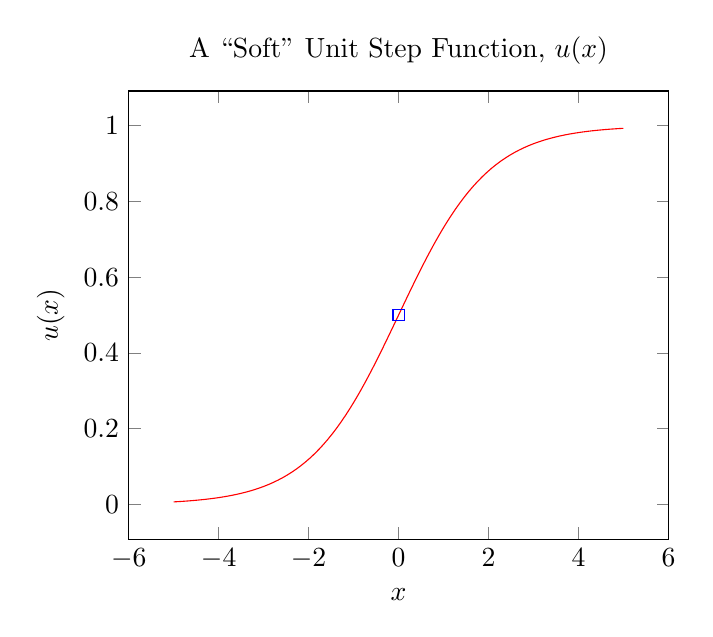
\begin{tikzpicture}
\begin{axis}[
title={A ``Soft" Unit Step Function, $u(x)$},
    xlabel={$x$},
    ylabel={$u(x)$}]
\addplot[samples=100, color=red]{1/(1 + exp(-x))};
\addplot[
    color=blue,
    mark=square,
    ]
    coordinates {
    (0,0.5)
    };
\end{axis}
\end{tikzpicture}
\end{center}
The gradient of this brightness across the edge, given by $\nabla u(x)$ (or $\der{u}{x}$ in one dimension), is then given by the following.  Notice that the location of the maximum matches the inflection point in the graph above:
\begin{center}
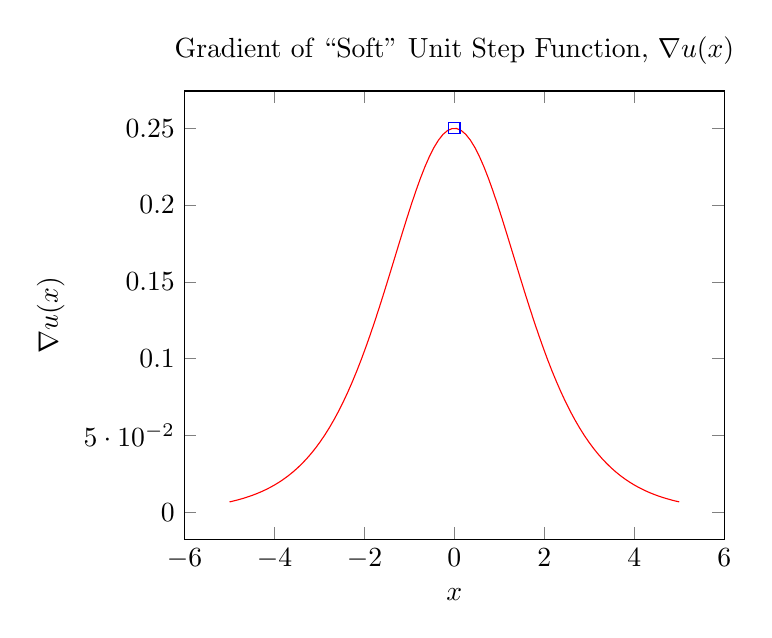
\begin{tikzpicture}
\begin{axis}[
title={Gradient of ``Soft" Unit Step Function, $\nabla u(x)$},
    xlabel={$ x$},
    ylabel={$\nabla u(x)$}]
\addplot[samples=100, color=red]{exp(-x)/(1 + exp(-x))^2};
\addplot[
    color=blue,
    mark=square,
    ]
    coordinates {
    (0,0.25)
    };
\end{axis}
\end{tikzpicture}
\end{center}
As we mentioned above, we can find the location of this edge by looking at where the second derivative of brightness crosses zero, a.k.a. where $\nabla (\nabla u(x)) = \nabla^2 u(x) = 0$.  Notice that the location of this zero is given by the same location as the inflection point of $u(x)$ and the maximum of $\nabla u(x)$:
\begin{center}
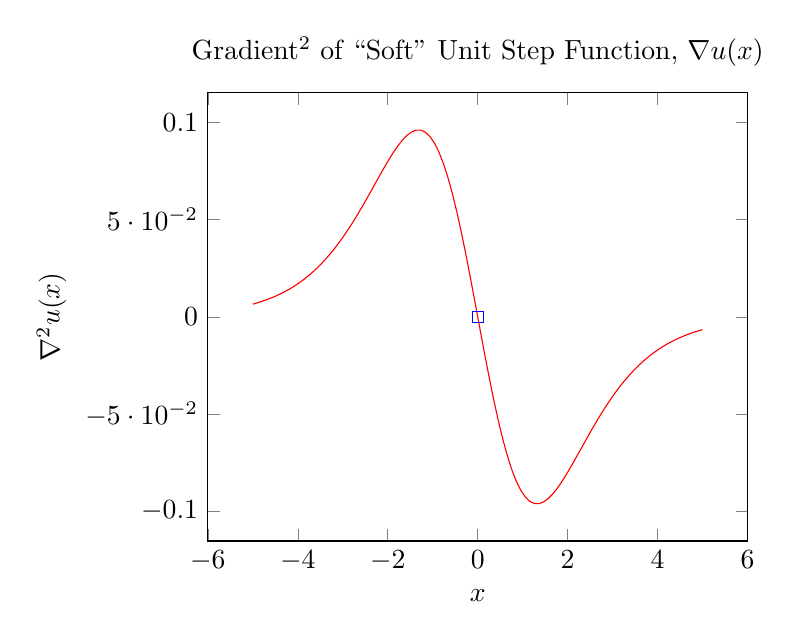
\begin{tikzpicture}
\begin{axis}[
title={Gradient$^2$ of ``Soft" Unit Step Function, $\nabla u(x)$},
    xlabel={$x$},
    ylabel={$\nabla^2 u(x)$}]
\addplot[samples=100, color=red]{(-exp(-x)*(1+exp(-x))^2 + exp(-x)*2*(1+exp(-x))*exp(-x))/(1+exp(-x))^4};
\addplot[
    color=blue,
    mark=square,
    ]
    coordinates {
    (0,0.0)
    };
\end{axis}
\end{tikzpicture}
\end{center}
For those curious, here is the math behind this specific function, assuming a sigmoid for $u(x)$:
\begin{enumerate}
    \item $u(x) = \frac{1}{1 + \exp{(-x)}}$
    \item $\nabla u(x) = \der{u}{x} = \frac{d}{dx}\Big(\frac{1}{1 + \exp{-x}}\Big) = \frac{\exp(-x)}{(1 + \exp(-x))^2}$
    \item $\nabla^2 u(x) = \dder{u}{x} = \frac{d}{dx}(\frac{\exp(-x)}{(1 + \exp(-x))^2}) = \frac{-\exp(-x)(1+\exp(-x))^2 + 2\exp(-x)(1+\exp(-x))\exp(-x)}{(1+\exp(-x))^4}$
\end{enumerate}
Building on top of this framework above, let us now move on to brightness gradient estimation.
\subsubsection{Brightness Gradient Estimation}
This component of this studied edge detection framework estimates the magnitude and direction of the brightness gradient.  Let us look at how this is derived for different filters: \\ \\
\textbf{Robert's Cross Gradient}: Since this estimates derivatives at 45 degree angles, the pixels are effectively further apart, and this means there will be a constant of proportionality difference between the magnitude of the gradient estimated here and with a normal $(x, y)$ coordinate system:
\begin{align*}
    \sqrt{E^{2}_{x'} + E^{2}_{y'}} \propto \sqrt{E^2_x + E^2_y} &&
\end{align*}
Next, we will look at the Sobel operator.  For this analysis, it will be helpful to recall the following result from Taylor Series:
\begin{align*}
    f(x+\delta x) = f(x) + \delta xf'(x) + \frac{(\delta x)^2}{2!}f''(x) + \frac{(\delta x)^3}{3!}f'''(x) + \frac{(\delta x)^4}{24}f^{(4)}(x) + ... = \sum_{i=0}^{\infty}\frac{(\delta x)^if^{(i)}(x)}{i!}, \;\;\text{where} \; 0! \delteq 1 &&
\end{align*}
Let us first consider the simple two-pixel difference operator (in the x-direction/in the one-dimensional case), \\ i.e. $\der{E}{x} \rightarrow K_x = \frac{1}{\delta}(-1 \; 1)$.  Let us look at the \textbf{forward difference} and \textbf{backward difference} when this operator is applied:
\begin{enumerate}
    \item \textbf{Forward Difference}: $\pd{E}{x} \approx \frac{f(x+\delta x)-f(x)}{\delta x} = f'(x) + \frac{\delta x}{2}f''(x) + \frac{(\delta x)^2}{6}f'''(x) + ...$
    \item \textbf{Backward Difference}: $\pd{E}{x} \approx \frac{f(x)-f(x-\delta x)}{\delta x} = -f'(x) - \frac{\delta x}{2}f''(x) + \frac{(\delta x)^2}{6}f'''(x) + ...$
\end{enumerate}
Notice that for both of these, if $f''(x)$ is large, i.e. if $f(x)$ is nonlinear, then we will have second-order error terms that appear in our estimates.  In general, we want to aim for removing these lower-order error terms.  If we average the forward and backward differences, however, we can see that these second-order error terms disappear:
\begin{align*}
    \frac{\frac{f(x+\delta x)-f(x)}{\delta x} + \frac{f(x)-f(x-\delta x)}{\delta x}}{2} = f'(x) + \frac{(\delta x)^2}{6}f'''(x) + ... &&
\end{align*}
Now we have increased the error term to 3rd order, rather than 2nd order!  As a computational molecule, this higher-order filter Sobel operator looks like $\der{E}{x} \rightarrow K_x = \frac{1}{2\delta}(-1 \; 0 \; 1)$.  But we can do even better!  So long as we do not need to have a pixel at our proposed edge, we can use a filter of three elements spanning $(x-\frac{\delta}{2} \; x \; x + \frac{\delta}{2})$.  There is no pixel at $x$ but we can still compute the derivative here.  This yields an error that is 0.25 the error above due to the fact that our pixels are $\frac{\delta}{2}$ apart, as opposed to $\delta$ apart:
\begin{align*}
    \text{error} = \frac{(\frac{x\delta}{2})^2}{6}f'''(x) &&
\end{align*}
This makes sense intuitively, because the closer together a set of gradient estimates are, the more accurate they will be.  We can incorporate $y$ into the picture, making this amenable for two-dimensional methods as desired, by simply taking the center of four pixels, given for each dimension as:
\begin{align*}
    & \pd{E}{x} \approx K_x = \frac{1}{2\delta_x}\begin{bmatrix}-1 & 1 \\ -1 & 1\end{bmatrix} \\
    & \pd{E}{y} \approx K_y = \frac{1}{2\delta_y}\begin{bmatrix}-1 & -1 \\ 1 & 1\end{bmatrix} &&
\end{align*}
The proposed edge is in the middle of both of these kernels, as shown below:
\begin{figure}[H]
    \centering
    \includegraphics[width=6cm]{figures/xy_filters.png}
    \caption{We can estimate the brightness gradient with minimal error by estimating it at the point at the center of these 2D filters.}
    \label{fig:my_label}
\end{figure}
Estimating these individually in each dimension requires 3 operations each for a total of 6 operations, but if we are able to take the common operations from each and combine them either by addition or subtraction, this only requires 4 operations.  Helpful especially for images with lots of pixels. \\ \\
Next, we will discuss the 3-by-3 Sobel operator.  We can think of this Sobel operator (in each dimension) as being the discrete convolution of a 2-by-2 horizontal or vertical highpass/edge filer with a smoothing or averaging filter:
\begin{enumerate}
    \item \textbf{x-direction}: $\frac{1}{2\delta_x}\begin{bmatrix}-1 & 1 \\ -1 & 1\end{bmatrix} \otimes \begin{bmatrix}1 & 1 \\ 1 & 1\end{bmatrix} = 
    \begin{bmatrix}-1 & 0 & 1 \\ -2 & 0 & 2 \\ -1 & 0 & 1 \end{bmatrix}$
    \item \textbf{y-direction}: $\frac{1}{2\delta_y}\begin{bmatrix}-1 & -1 \\ 1 & 1\end{bmatrix} \otimes \begin{bmatrix}1 & 1 \\ 1 & 1\end{bmatrix} = 
    \begin{bmatrix}-1 & -2 & -1 \\ 0 & 0 & 0 \\ 1 & 2 & 1 \end{bmatrix}$
\end{enumerate}
A few notes about the derivation above:
\begin{itemize}
    \item The convolution used is a ``padded convolution" [3], in which, when implemented, when the elements of the filter/kernel (in this case, the averaging kernel) are not aligned with the image, they are simply multiplied by zero.  Zero padding is the most common padding technique, but there are other techniques as well, such as wraparound padding.
    \item This approach avoids the half-pixel (in which we estimate an edge that is not on a pixel) that was cited above.
    \item Smoothing/averaging is a double edge sword, because while it can reduce/remove high-frequency noise by filtering, it can also introduce undesirable blurring.
\end{itemize}
Next, we will look at how the brightness gradient is converted from Cartesian to Polar coordinates:
\begin{align*}
    & (E_x, E_y) \rightarrow (E_0, E_{\theta}) \\
    & E_0 = \sqrt{E^2_x + E^2_y} \\
    & E_{\theta} = \tan^{-1}\Big(\frac{E_y}{E_y}\Big) &&
\end{align*}
Finally, we conclude this lecture by looking at appropriate values of $s$ for quadratic and triangular functions.  This assumes we have three gradient measurements centered on $G_0$: (1) $G_{-}$, (2) $G_0$, and (3) $G_{+}$.  Let us look at the results for these two types of functions:
\begin{enumerate}
    \item \textbf{Quadratic}: $s = \frac{G_{+} - G_{-}}{4(G_0 - \frac{1}{2}(G_{+}-G_{-}))}$, this results in $s \in [-\frac{1}{2}, \frac{1}{2}]$.
    \item \textbf{Triangular}: $s = \frac{G_{+} - G_{-}}{2(G_0 - \min(G_{+}, G_{-}))}$
\end{enumerate}
A few notes about these approaches:
\begin{itemize}
    \item Note that in each case, we only want to keep if the magnitude $G_0$ is a local maximum, i.e. $G_0 > G_{+}$ and $G_0 \geq G_{-}$.
    \item In the quadratic case, we can parameterize the curve with three data points using three degrees of freedom, i.e. $ax^2 + bx + c = 0$.  With this approach, $b \approx \text{first derivative}$ and $a \approx \text{second derivative}$.
\end{itemize}
\subsection{References}
\begin{enumerate}
    \item CORDIC Algorithm, https://www.allaboutcircuits.com/technical-articles/an-introduction-to-the-cordic-algorithm/
    \item Non-Maximum Supression, http://justin-liang.com/tutorials/canny/\#suppression
    \item Padded Convolution, https://medium.com/@ayeshmanthaperera/what-is-padding-in-cnns-71b21fb0dd7
\end{enumerate}

%%%%%%%%%%%%%%%%%%%%%%%%%%%%% LEC 12 %%%%%%%%%%%%%%%%%%%%%%%%%%%%%%%%%%%%%%%%%%%%%%%%
\section{Lecture 12: Blob analysis, Binary Image Processing, Use of Green's Theorem, Derivative and Integral as Convolutions}
In this lecture, we will continue our discussion of intellectual property, and how it relevant for all scientists and engineers.  We will then elaborate on some of the specific machine vision techniques that were used in this patent, as well as introduce some possible extensions that could be applicable for this patent as well.
\subsection{Types of Intellectual Property}
Though it is not related to the technical content of machine vision, being familiar with different types and degrees of intellectual property (IP) is crucial to professional success.  Below, we discuss some of these different types of intellectual property.
\begin{itemize}
    \item \textbf{Patents}: One major type of these is utility and design patents.  In these, the authors are required to disclose the ``best mode" of performance.  For convenience, here are some notes on patents from our previous lecture:
    \begin{itemize}
        \item Can be thought of as a ``contract with society" - you get a limited monopoly on your idea, and in turn, you publish the technical details of your approach.
        \item Can help to reduce litigation and legal fees.
        \item Can be used by large companies as ``ammunition" for ``patent wars".
    \end{itemize}
    Some ``rules" of patents:
    \begin{itemize}
        \item No equations are included in the patent (no longer true)
        \item No greyscale images - only black and white
        \item Arcane grammar is used for legal purposes - ``comprises", ``apparatus", ``method", etc.
        \item References of other patents are often included - sometimes these are added by the patent examiner, rather than the patent authors
        \item Most patents end with something along the lines of ``this is why our invention was necessary" or ``this is the technical gap our invention fills"
        \item Software is not patentable - companies and engineers get around this by putting code on hardware and patenting the ``apparatus" housing the code.
        \item It is also common to include background information (similar to related literature in research).
    \end{itemize}
    \item \textbf{Copyright}:
    \begin{itemize}
        \item Books, song recordings, choreographs
        \item Exceptions: presenting (fractional pieces of) information from another author
    \end{itemize}
    \item \textbf{Trademarks}:
    \begin{itemize}
        \item Must be unique for your field (e.g. Apple vs. Apple).
        \item Cannot use common words - this is actually one reason why many companies have slightly misspelled combinations of common words.
        \item Can use pictures, character distortions, and color as part of the trademark.
        \item No issues if in different fields.
    \end{itemize}
    \item \textbf{Trade Secret}
    \begin{itemize}
        \item No protections, but not spilled, lasts forever
        \item Can enforce legal recourse with Non-Disclosure Agreement (NDA)
    \end{itemize}
\end{itemize}
\subsection{Edge Detection Patent Methodologies}
For this next section, we will direct our attention toward covering concepts that were discussed in the edge detection patent (6,408,109).  Each of these sections will be discussed in further detail below.  Before we get into the specifics of the patent again, it is important to point out the importance of edge detection for higher-level machine vision tasks, such as:
\begin{itemize}
    \item Attitude (pose estimation) of an object
    \item Object recognition
    \item Determining to position
\end{itemize}
We will touch more on these topics in later lectures.
\subsubsection{Finding Edge with Derivatives}
Recall that we find a proposed edge by finding an \textbf{inflection point} of the brightness $E(x,y)$.  The following methods for finding this point are equivalent:
\begin{itemize}
    \item Finding an inflection point of brightness $E(x,y)$.
    \item Finding maximum of brightness gradient magnitude/first derivative $|\nabla E(x,y)|$.
    \item Finding zero crossing of Laplacian/second derivative $\nabla^2 E(x,y)$.
\end{itemize}
For building intuition, last time we used the following example of $u(x) = \sigma(x) = \frac{1}{1 + \exp(-x)}$:
\begin{center}
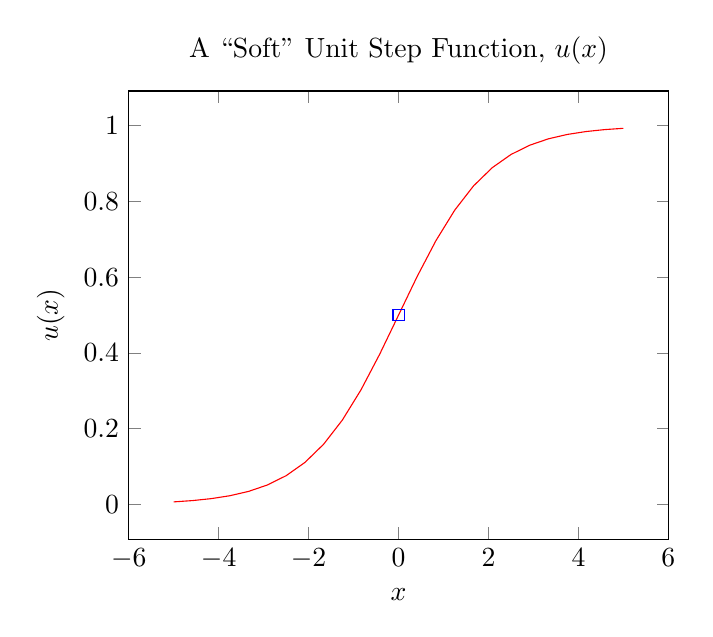
\begin{tikzpicture}
\begin{axis}[
title={A ``Soft" Unit Step Function, $u(x)$},
    xlabel={$x$},
    ylabel={$u(x)$}]
\addplot[color=red]{1/(1 + exp(-x))};
\addplot[
    color=blue,
    mark=square,
    ]
    coordinates {
    (0,0.5)
    };
\end{axis}
\end{tikzpicture}
\end{center}
The gradient of this brightness across the edge, given by $\nabla u(x)$ (or $\der{u}{x}$ in one dimension), is then given by the following.  Notice that the location of the maximum matches the inflection point in the graph above:
\begin{center}
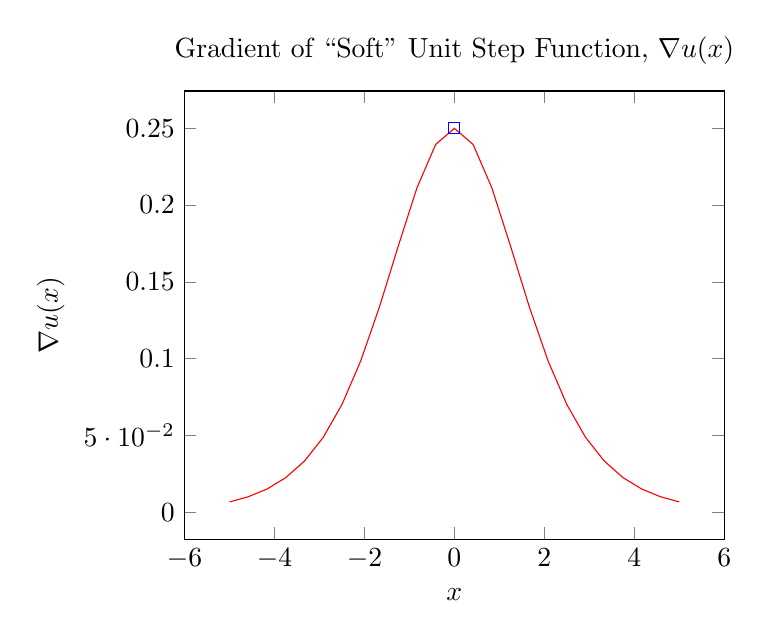
\begin{tikzpicture}
\begin{axis}[
title={Gradient of ``Soft" Unit Step Function, $\nabla u(x)$},
    xlabel={$ x$},
    ylabel={$\nabla u(x)$}]
\addplot[color=red]{exp(-x)/(1 + exp(-x))^2};
\addplot[
    color=blue,
    mark=square,
    ]
    coordinates {
    (0,0.25)
    };
\end{axis}
\end{tikzpicture}
\end{center}
As we mentioned above, we can find the location of this edge by looking at where the second derivative of brightness crosses zero, a.k.a. where $\nabla (\nabla u(x)) = \nabla^2 u(x) = 0$.  Notice that the location of this zero is given by the same location as the inflection point of $u(x)$ and the maximum of $\nabla u(x)$:
\begin{center}
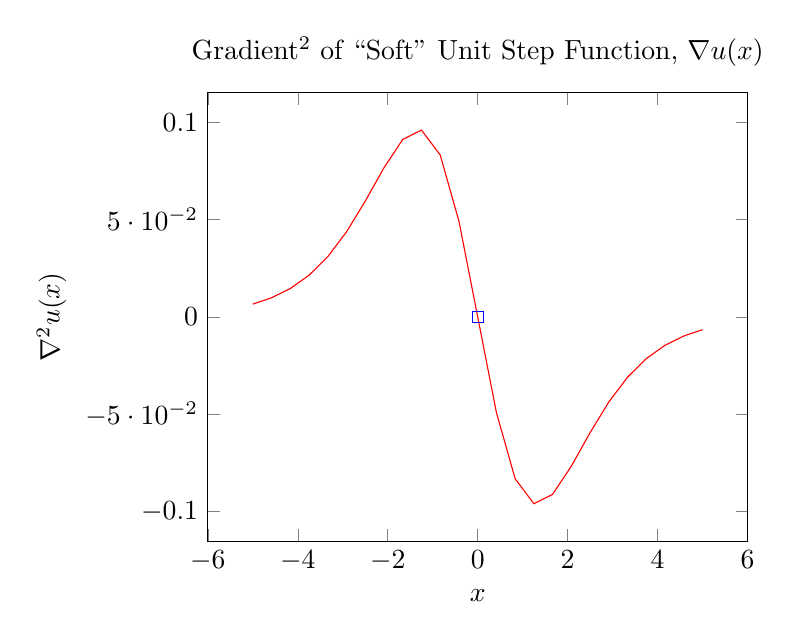
\begin{tikzpicture}
\begin{axis}[
title={Gradient$^2$ of ``Soft" Unit Step Function, $\nabla u(x)$},
    xlabel={$x$},
    ylabel={$\nabla^2 u(x)$}]
\addplot[color=red]{(-exp(-x)*(1+exp(-x))^2 + exp(-x)*2*(1+exp(-x))*exp(-x))/(1+exp(-x))^4};
\addplot[
    color=blue,
    mark=square,
    ]
    coordinates {
    (0,0.0)
    };
\end{axis}
\end{tikzpicture}
\end{center}
For those curious, here is the math behind this specific function, assuming a sigmoid for $u(x)$:
\begin{enumerate}
    \item $u(x) = \frac{1}{1 + \exp{(-x)}}$
    \item $\nabla u(x) = \der{u}{x} = \frac{d}{dx}\Big(\frac{1}{1 + \exp{-x}}\Big) = \frac{\exp(-x)}{(1 + \exp(-x))^2}$
    \item $\nabla^2 u(x) = \dder{u}{x} = \frac{d}{dx}(\frac{\exp(-x)}{(1 + \exp(-x))^2}) = \frac{-\exp(-x)(1+\exp(-x))^2 + 2\exp(-x)(1+\exp(-x))\exp(-x)}{(1+\exp(-x))^4}$
\end{enumerate}
\subsubsection{More on ``Stencils"/Computational Molecules}
Recall that we can use finite differences [1] in the forms of ``stencils" or computational molecules to estimate derivatives in our images.  For this patent, the authors used this framework to estimate the brightness gradient in order to find edges.  For instance, partial derivative of brightness w.r.t. $x$ can be estimated by
\begin{enumerate}
    \item $E_x = \frac{1}{\epsilon}\begin{bmatrix}-1 & 1\end{bmatrix}$
    \item $E_x = \frac{1}{2\epsilon}\begin{bmatrix}-1 & 0 & 1\end{bmatrix}$
    \item $E_x = \frac{1}{2\epsilon}\begin{bmatrix}-1 & 1 \\
                                                    -1 & 1
                                     \end{bmatrix}$
\end{enumerate}
Where for molecule 2, the best point for estimating derivatives lies directly in the center pixel, and for molecules 1 and 3, the best point for estimating derivatives lies halfway between the two pixels. \\ \\
\textbf{How do we analyze the efficacy of this approach}?
\begin{enumerate}
    \item \textbf{Taylor Series}: From previous lectures we saw that we could use averaging to reduce the error terms from 2nd order derivatives to third order derivatives.  This is useful for analytically determining the error.
    \item \textbf{Test functions}: We will touch more on these later, but these are helpful for testing your derivative estimates using analytical expressions, such as polynomial functions.
    \item \textbf{Fourier domain}: This type of analysis is helpful for understanding how these ``stencils"/molecules affect higher (spatial) frequency image content.
\end{enumerate}
Note that derivative estimators can become quite complicated for high-precision estimates of the derivative, even for low-order derivatives.  We can use large estimators over many pixels, but we should be mindful of the following tradeoffs:
\begin{itemize}
    \item We will achieve better noise smoothing/suppression by including more measured values.
    \item Larger derivative estimators linearly (1D)/quadratically (2D) increase the amount of computation time needed.
    \item  Features can also affect each other - e.g. a large edge detection estimator means that we can have two nearby edges affecting each other.
\end{itemize}
We can also look at some derivative estimators for higher-order derivatives.  For 2nd-order derivatives, we just apply another derivative operator, which is equivalent to convolution of another derivative estimator ``molecule":
\begin{align*}
    \pddop{x}(\cdot) = \pdop{x}\Big(\pd{(\cdot)}{x}\Big) \Longleftrightarrow \frac{1}{\epsilon} \begin{bmatrix}-1 & 1\end{bmatrix} \otimes \frac{1}{\epsilon} \begin{bmatrix}-1 & 1\end{bmatrix} = \frac{1}{\epsilon^2}\begin{bmatrix}1 & -2 & 1\end{bmatrix} &&
\end{align*}
For deriving the sign here and understanding why we have symmetry, remember that convolution ``flips" one of the two filters/operators! \\ \\
\textbf{Sanity Check}: Let us apply this to some functions we already know the 2nd derivative of. \\ \\
\begin{itemize}
    \item $f(x) = x^2$:
        \begin{align*}
            f(x) = x^2 \\
            f'(x) = 2x \\
            f''(x) = 2 &&
        \end{align*}
        Applying the 2nd derivative estimator above to this function:
        \begin{align*}
            \begin{bmatrix}1 & -2 & 1\end{bmatrix} \otimes \frac{1}{\epsilon} \begin{bmatrix}f(-1) = 1 & f(0) = 0 & f(1) = 1\end{bmatrix} = \frac{1}{\epsilon^2}((1*1) + (-2*0) + (1*1)) = \frac{1}{\epsilon^2}(1 + 0 + 1) = 1 * 2 = 2 &&
        \end{align*}
        Where we note that $\epsilon = 1$ due to the pixel spacing.  This is equivalent to $f''(x) = 2$.
    \item $f(x) = x$:
        \begin{align*}
            f(x) = x \\
            f'(x) = 1 \\
            f''(x) = 0 &&
        \end{align*}
        Applying the 2nd derivative estimator above to this function:
        \begin{align*}
            \begin{bmatrix}1 & -2 & 1\end{bmatrix} \otimes \frac{1}{\epsilon} \begin{bmatrix}f(-1) = -1 & f(0) = 0 & f(1) = 1\end{bmatrix} = \frac{1}{\epsilon^2}((1*-1) + (-2*0) + (1*1)) = \frac{1}{\epsilon^2}(-1 + 0 + 1) = 0 &&
        \end{align*}
        Where we note that $\epsilon = 1$ due to the pixel spacing.  This is equivalent to $f''(x) = 0$.
    \item $f(x) = 1$:
        \begin{align*}
            f(x) = 1 \\
            f'(x) = 0 \\
            f''(x) = 0 &&
        \end{align*}
        Applying the 2nd derivative estimator above to this function:
        \begin{align*}
            \begin{bmatrix}1 & -2 & 1\end{bmatrix} \otimes \frac{1}{\epsilon} \begin{bmatrix}f(-1) = 1 & f(0) = 1 & f(1) = 1\end{bmatrix} = \frac{1}{\epsilon^2}((1*1) + (-2*1) + (1*1)) = \frac{1}{\epsilon^2}(1 + -2 + 1) = 0 &&
        \end{align*}
        Where we note that $\epsilon = 1$ due to the pixel spacing.  This is equivalent to $f''(x) = 0$.
\end{itemize}
\tetbf{In Practice}: As demonstrated in the example ``test functions" above, in general a good way to test an N$^{\text{th}}$ order derivative estimator is use polynomial test functions of arbitrary coefficients from order 0 up to order N.  For instance, to calculate 4th order derivative estimator, test:
\begin{enumerate}
    \item $f(x) = a$
    \item $f(x) = ax + b$
    \item $f(x) = ax^2 + bx + c$
    \item $f(x) = ax^3 + bx^2 + cx + d$
    \item $f(x) = ax^4 + bx^3 + cx^2 + dx + e$
\end{enumerate}
\textbf{Note}: For derivative estimator operators, the weights of the ``stencils"/computational molecules should add up to zero.  Now that we have looked at some of these operators and modes of analysis in one dimension, let us now look at 2 dimensions.
\subsubsection{Mixed Partial Derivatives in 2D}
First, it is important to look at the linear, shift-invariant property of these operators, which we can express for each quality:
\begin{itemize}
    \item \textbf{Shift-Invariant}: 
    \begin{align*}
        \derop{x}(f(x+\delta)) &= f'(x+\delta), \;\text{for some} \; \delta \in \mathbb{R}\\
        \text{Derivative of shifted function} \;&=\;\text{Derivative equivalently shifted by same amount} &&
    \end{align*}
    \item \textbf{Linear }: 
    \begin{align*}
        \derop{x}(af_1(x) + bf_2(x)) &= af'_1(x) + bf'_2(x) \;\text{for some} \; a,b \in \mathbb{R}\\
        \text{Derivative of scaled sum of two functions} \;&=\;\text{Scaled sum of derivatives of both functions} &&
    \end{align*}
\end{itemize}
We will exploit this \textbf{linear, shift-invariant} property frequently in machine vision.  Because of this joint property, we can treat derivative operators as convolutions in 2D:
\begin{align*}
    \pddmixedop{x}{y}(\cdot) = \pdop{x}\Big(\pdop{y}(\cdot)\Big) \Longleftrightarrow \frac{1}{\epsilon}\begin{bmatrix}-1 & 1\end{bmatrix} \otimes \frac{1}{\epsilon}\begin{bmatrix}1 \\ -1\end{bmatrix} = \frac{1}{\epsilon^2}\begin{bmatrix}-1 & +1 \\ +1 & -1\end{bmatrix} &&
\end{align*}
A few notes here:
\begin{itemize}
    \item The second operator corresponding to $E_y$ has been flipped in accordance with the convolution operator.
    \item If we project this derivative onto a ``diagonal view", we find that it is simply the second derivative of $x'$, where $x'$ is $x$ rotated 45 degrees counterclockwise in the 2D plane: $x' = x\cos 45 + y\cos 45 = \frac{\sqrt{2}}{2}x + \frac{\sqrt{2}}{2}y$. In other words, in this 45-degree rotated coordinate system, $E_{x'x'} = E_{xy}$.
    \item \textbf{Intuition for convolution}: If convolution is a new concept for you, check out reference [2] \href{https://towardsdatascience.com/intuitively-understanding-convolutions-for-deep-learning-1f6f42faee1}{here}.  Visually, convolution is equivalent to ``flipping and sliding" one operator across all possible (complete and partial) overlapping configurations of the filters with one another.
\end{itemize}
\subsubsection{Laplacian Estimators in 2D}
The Laplacian $\nabla^2 \delteq \Delta = \pddop{x} + \pddop{y}$ is another important estimator in machine vision, and, as we discussed last lecture, is the \textbf{lowest-order rotationally-symmetric} derivative operator.  Therefore, our finite difference/computational molecule estimates should reflect this property if they are to be accurate.  Two candidate estimators of this operator are:
\begin{enumerate}
    \item \textbf{``Direct Edge"}: $\frac{1}{\epsilon^2}\begin{bmatrix}0 & 1 & 0 \\
                                                   1 & -4 & 1 \\
                                                   0 & 1 & 0
                                    \end{bmatrix}$
    \item \textbf{``Indirect Edge"}: $\frac{1}{2\epsilon^2}\begin{bmatrix}1 & 0 & 1 \\
                                                     0 & -4 & 0 \\
                                                     1 & 0 & 1
                                    \end{bmatrix}$
\end{enumerate}
Note that the second operator has a factor of $\frac{1}{2\epsilon^2}$ in front of it because the distance between edges is $\sqrt{2}$ rather than 1, therefore, we effectively have $\frac{1}{\epsilon'^2}$, where $\epsilon' = \sqrt{2}\epsilon$. \\ \\
How do we know which of these approximations is better?  We can go back to our analysis tools:
\begin{itemize}
    \item Taylor Series
    \item Test functions
    \item Fourier analysis
\end{itemize}
Intuitively, we know that neither of these estimators will be optimal, because neither of these estimators are rotationally-symmetric.  Let us combine these intelligently to achieve rotational symmetry.  Adding four times the first one with one times the second:
\begin{align*}
    4 \Big(\frac{1}{\epsilon^2}\begin{bmatrix}0 & 1 & 0 \\
                                                   1 & -4 & 1 \\
                                                   0 & 1 & 0
                                    \end{bmatrix}\Big) + 1 \Big(\frac{1}{2\epsilon^2}\begin{bmatrix}1 & 0 & 1 \\
                                                     0 & -4 & 0 \\
                                                     1 & 0 & 1
                                    \end{bmatrix}\Big) = \frac{1}{6\epsilon^2}\begin{bmatrix}1 & 4 & 1 \\
                                                                        4 & -20 & 4 \\
                                                                        1 & 4 & 1
                                                        \end{bmatrix} &&
\end{align*}
Using Taylor Series, we can show that this estimator derived from this linear combination of estimators above results in an error term that is \textbf{one derivative higher} than suing either of the individual estimators above, at the cost of more computation.  Note that the sum of all the entries here is zero, as we expect for derivative estimators. \\ \\
For a hexagonal grid, this is scaled by $\frac{1}{2\epsilon^2}$ and has entries of all 1s on the outer ring, and an entry of -6 in the center.  An example application of a hexagonal grid - imaging black holes!  Leads to $\frac{4}{\pi}$ greater efficiency. \\ \\
As food for thought, what lowest-order rotationally-symmetric \textit{nonlinear} operators?
\begin{align*}
    \sqrt{E^2_{x'} + E^2_{y'}} = \sqrt{E^2_{x} + E^2_{y}} \;\;\text{Where this is the l2 normal of the estimated brightness gradient} &&  
\end{align*}
\subsubsection{Non-Maximum Suppression}
Another technique leveraged in this patent was \textbf{Non-Maximum Suppression (NMS)}.  Idea: Apply edge detector estimator operator everywhere - we will get a small response in most places, so what if we just threshold?  This is an instance of \textbf{early decision-making}, because once we take out these points, they are no longer considered edge candidates in downstream steps. \\ \\
It turns out the authors discourage thresholding, and in their work they remove all but the maximum estimated gradient (note that this is quantized at the octant level).  Note that the quantized gradient direction is perpendicular to the edge.  In this case, for a candidate gradient point $G_0$ and the adjacent pixels $G_{-}$ and $G_{+}$, we must have:
\begin{align*}
    G_0 > G_{-}, G_0 \geq G_{+} &&
\end{align*}
This forces $-\frac{1}{2} \leq s \leq \frac{1}{2}$.
Note that we have the asymmetric inequality signs to break ties arbitrarily.  Next we plot the quantized profile that has been interpolated parabolically - i.e. sub-pixel interpolation.
\subsubsection{Plane Position}
Note that we have not yet done any thresholding.  How can we improve this, given that we quantized the edge gradient direction?  Could we try not quantizing the edge direction?  If we have the true gradient direction, we can find the intersection of this line with the edge (at 90 degrees to the edge gradient) to find a better solution.  \\ \\
To find this point above (please take a look at the handwritten lecture notes for this lecture), we project from the quantized gradient direction to the actual gradient direction.  This is the ``plane position" component.
\subsubsection{Bias Compensation}
Another component of the patent focuses on the interpolation technique used for sub-pixel gradient plotting for peak finding.  To find an optimal interpolation technique, we can plot $s$ vs. $s'$, where $s' = s|2s|^b$, where $b \in \mathbb{N}$ is a parameter that determines the relationship between $s$ and $s'$.  \\ \\
In addition to cubic interpolation, we can also consider piecewise linear interpolation with ``triangle" functions.  For some different values of $b$:
\begin{itemize}
    \item $b = 0 \rightarrow s' = s$
    \item $b = 1 \rightarrow s' = 2\text{sign}(s)s^2$
    \item $b = 2 \rightarrow s' = 4\text{sign}(s)s^3$
\end{itemize}
Where different interpolation methods give us different values of $b$.
\subsubsection{Edge Transition and Defocusing Compensation}
Another point of motivation: most edge detection results depend on the actual edge transition.   Why are edges fuzzy (note that some degree of fuzziness is needed to prevent aliasing)?  One major cause of fuzziness is ``defocusing", in which the image plane and ``in focus" planes are slightly off from one another.  This causes a ``pillbox" of radius $R$ to be imaged (see handwritten lecture notes), rather than the ideal case of an impulse function $\delta(x,y)$.  This radius is determined by:
\begin{align*}
    R = \delta\frac{d^2}{f} \;(\textbf{Point Spread Function (PSF)}) &&
\end{align*}
This pillbox image is given mathematically by:
\begin{align*}
    \frac{1}{\pi R^2}(1 - u(r-R)) &&
\end{align*}
Where $u(\cdot)$ is the unit step function.
Where $f$ is the focal length of the lens, $d$ is the diameter of the lens (assumed to be conic), and $\delta$ is the distance along the optical axis between the actual image plane and the ``in focus" plane.
\subsubsection{Multiscale}
\textbf{Note}: We will discuss this in greater detail next lecture. \\ \\
Multiscale is quite important in edge detection, because we can have edges at different scales.  To draw contrasting examples, we could have an image such that:
\begin{itemize}
    \item We have very sharp edges that transition over $\approx$ only 1 pixel
    \item We have blurry edges that transition over many pixels
\end{itemize}
\subsubsection{Effect on Image Edge}
Here is one possible extension not included in the edge detection patent. \\ \\
We can slide a circle across a binary image - the overlapping regions inside the circle between the 1-0 edge controls how bright things appear.  We can use this technique to see how accurately the algorithm plots the edge position - this allows for error calculation since we have ground truth results that we can compute using the area of the circle.  Our area of interest is given by the area enclosed by the chord whose radial points intersect with the binary edge:
\begin{align*}
    & A = R^2\theta - \frac{2\sqrt{R^2-X^2}X}{2} \\
    & \theta = \arctan\Big(\frac{\sqrt{R^2-x^2}}{x}\Big) &&
\end{align*}
Another way to analyze this is to compute the analytical derivatives of this brightness function:
\begin{enumerate}
    \item $\pd{E}{x} = 2\sqrt{R^2 - x^2}$
    \item $\pdd{E}{x} = \frac{-2x}{\sqrt{R^2 - x^2}}$
\end{enumerate}
What can we do with this?  We can use this as input into our algorithm to compute teh error and \textbf{compensate} for the degree of defocusing of the lens.  In practice, there are other factors that lead to fuzzy edge profiles aside from defocusing, but this defocusing compensation helps.
\subsubsection{Addressing Quantization of Gradient Directions}
Here is another possible extension not included in the edge detection patent. \\ \\
Recall that because spaces occurs in two sizes (pixel spacing and $\sqrt{2}$ pixel spacing), we need to sample in two ways, which can lead to slightly different error contributions.  We do not want quantized gradient directions.  To do this, we can just interpolate values $G_{-}, G_0, G_{+}$ along the true edge gradient!  \\ \\
\textbf{Linear 1D Interpolation}: 
\begin{align*}
    \tilde{f}(x) = \frac{f(a)(b-x) + f(b)(x-a)}{b-a} &&
\end{align*}
We can also leverage more sophisticated interpolation methods, such as \textbf{cubic spline}. \\ \\
\textbf{Why did the authors not leverage this interpolation strategy?}
\begin{itemize}
    \item this requires the spacing of any level, i.e. not just pixel and $\sqrt{2}$ pixel spacing, but everything in between.
    \item Since you interpolate, you are not using measured values.  Introduces some uncertainty that may be too much to achieve 1/40$\text{th}$ pixel accuracy.
\end{itemize}
What can we do to address this?  $\rightarrow$ \textbf{Project gradient onto unit circle!}  This requires 2D interpolation, which can be done with methods such as bilinear or bicubic interpolation.
\subsubsection{CORDIC}
As we discussed in the previous lecture, CORDIC is an algorithm used to estimate vector direction by iteratively rotating a vector into a correct angle.  For this patent, we are interested in using CORDIC to perform a change of coordinates from cartesian to polar:
\begin{align*}
    (E_x, E_y) \rightarrow (E_0, E_{\theta}) &&
\end{align*}
\textbf{Idea}: Rotate a coordinate system to make estimates using test angles iteratively.  Note that we can simply compute these with square roots and arc tangents, but these can be prohibitively computationally-expensive:
\begin{align*}
    & E_0 = \sqrt{E^2_x + E^2_y} \\
    & E_{\theta} = \arctan\Big(\frac{E_y}{E_x}\Big) &&
\end{align*}
Rather than computing these directly, it is faster to iteratively solve for the desired rotation $\theta$ by taking a sequence of iterative rotations $\{\theta_i\}_{i=1, 2, \cdots}^{n}$.  The iterative updates we have for this are, in matrix-vector form:
\begin{align*}
    \begin{bmatrix}E^{(i+1)}_x \\ E^{(i+1)}_y \end{bmatrix} & = \begin{bmatrix}\cos\theta_i & \sin\theta_i \\ -\sin\theta_i & \cos\theta_i\end{bmatrix}\begin{bmatrix}E^{(i)}_x \\ E^{(i)}_y \end{bmatrix} \\
    \text{Gradients at next step} & = \;\text{Rotation R by} \; \theta_i \times \;\text{Gradients at current step} &&
\end{align*}
How do we select $\{\theta_i\}_{i=1, 2, \cdots}^{n}$?  We can select progressively smaller angles.  We can accept the candidate angle and invoke the iterative update above if each time the candidate angle reduces $|E_y|$ and increases $|E_x|$. \\ \\
The aggregate rotation $\theta$ is simply the sum of all these accepted angles: $\theta = \sum_{i}\theta_i$ \\ \\
One potential practical issue with this approach is that it involves a significant number of multiplications.  How can we avoid this?  We can pick the angles carefully - i.e. if our angles are given successively by $\frac{\pi}{2}$, $\frac{\pi}{4}$, $\frac{\pi}{8}$, ..., then:
\begin{align*}
    \frac{\sin\theta_u}{\cos\theta_i} = \frac{1}{2^i} \rightarrow \;\text{rotation matrix becomes}: \; \frac{1}{\cos\theta_i}\begin{bmatrix}1 & 2^{-i} \\ -2^{-i} & 1\end{bmatrix} &&
\end{align*}
Note that this reduces computation to 2 additions per iteration.  Angle we turn through becomes successively smaller:
\begin{align*}
    \cos\theta_i = \sqrt{1 + \frac{1}{2^{2i}}} \rightarrow R = \prod_{i}\cos\theta_i = \prod_{i}\sqrt{1 + \frac{1}{2^{2i}}} \approx 1.16 \;(\text{precomputed}) &&
\end{align*}

\subsection{References}
\begin{enumerate}
    \item Finite Differences, https://en.wikipedia.org/wiki/Finite\_difference
    \item Convolution, https://towardsdatascience.com/intuitively-understanding-convolutions-for-deep-learning-1f6f42faee1
\end{enumerate}

%%%%%%%%%%%%%%%%%%%%%%%%%%%%% LEC 13 %%%%%%%%%%%%%%%%%%%%%%%%%%%%%%%%%%%%%%%%%%%%%%%%
\section{Lecture 13: Object detection, Recognition and Pose Determination, PatQuick (US 7,016,539)}
In this lecture, we will begin by looking at some general problems for object detection and pose estimation of objects in an image, and also look at some optimization algorithms we can use for finding optimal matches between a ``master image" / template image, which is the object we look for, and this object in another image (perhaps in a scene).  We then look at a patent describing some of the approaches taken to solve some of these aforementioned tasks.
\subsection{Motivation \& Preliminaries for Object Detection/Pose Estimation}
Object detection and pose estimation builds on top of previous machine vision tasks we have covered.  Some specific tasks include:
\begin{itemize}
    \item Object detection - i.e. detect and locate object in an image
    \item Recognize object
    \item Determine pose of detected/recognized object
    \item Inspect object
\end{itemize}
\textbf{Motivation for these approaches}: In machine vision problems, we often manipulate objects in the world, and we want to know what and where these objects are in the world.  In the case of these specific problems, we assume prior knowledge of the precise edge points of these objects (which, as we discussed in the two previous lectures, we know how to compute!)
\subsubsection{``Blob Analysis"/"Binary Image Processing"}
We can use thresholding and other algorithms such as finding a convex hull to compute elements of an object in a binary image (black/white) such as:
\begin{itemize}
    \item Area (moment order 0)
    \item Perimeter
    \item Centroid (moment order 1)
    \item ``Shape" (generalization of different-order moments)
    \item Euler number - In this case this is the number of blobs minus number of holes
\end{itemize}
A few notes about computing these different quantities of interest:
\begin{itemize}
    \item We have seen from previous lectures that we can compute some of these elements, such as perimeter, using \textbf{Green's Theorem}.  We can also accomplish this with \textbf{counting} - can be done simply by counting pixels based off of whether their pixel is a 0 or 1.
    \item However, the issue with these approaches is that they require \textbf{thresholding} - i.e. removing points from any further consideration early on the process and possibly without all information available; essentially removing potentially viable points too early.
    \item \textbf{Shape}: As introduced above, shape is often computed by computing moments of any order.  Recall the definition of moments of a 2D shape:
    \begin{enumerate}
        \item \textbf{O-order}: $\iint_DE(x,y)dxdy \rightarrow$ \textbf{Area}
        \item \textbf{1-order}: $\iint_DE(x,y)xydxdy \rightarrow$ \textbf{Centroid}
        \item \textbf{2-order}: $\iint_DE(x,y)x^2y^2dxdy \rightarrow$ \textbf{Dispersion} \\
        $\vdots$
        \item \textbf{k-order}: $\iint_DE(x,y)x^ky^kdxdy$
    \end{enumerate}\
    \item Note that these methods are oftentimes applied to \textbf{processed}, not \textbf{raw} images.
\end{itemize}
\subsubsection{Binary Template}
We will discuss this more later, but this is crucial for the patent on object detection and pose estimation that we will be discussing today.  A binary template is:
\begin{itemize}
    \item A ``master image" to define the object of interest that we are trying to detect/estimate the pose of
    \item You will have a template of an object that you can recognize the object and get the pose/attitude.
\end{itemize}
\subsubsection{Normalized Correlation}
This methodology also plays a key role in the patent below. \\ \\
\textbf{Idea}: Try all possible positions/configurations of the pose space to create a match between the template and runtime image of the object.  If we are interested in the squared distance between the displaced template and the image in the other object (for computational and analytic simplicity, let us only consider rotation for now), then we have the following optimization problem:
\begin{align*}
    \min_{\delta_x, \delta_y}\iint_{D}(E_1(x-\delta_x, y-\delta_y)-E_2(x,y))^2dxdy &&
\end{align*}
Where we have denoted the two images separately as $E_1$ and $E_2$. \\ \\
In addition to framing this optimization mathematically as minimizing the squared distance between the two images, we can also conceptualize this as maximizing the correlation between the displaced image and the other image:
\begin{align*}
    \max_{\delta_x, \delta_y}\iint_{D}E_1(x-\delta_x, y-\delta_y)E_2(x,y)dxdy &&
\end{align*}
We can prove mathematically that the two are equivalent.  Writing out the first objective as $J(\delta_x, \delta_y)$ and expanding it:
\begin{align*}
    J(\delta_x, \delta_y) & = \iint_{D}(E(x-\delta_x, y-\delta_y)-E_2(x,y))^2dxdy \\
    & = \iint_{D}(E^2_1(x-\delta_x, y-\delta_y) -2\iint_DE_1(x-\delta_x, y-\delta_y)E_2(x,y)dxdy + \iint_DE^2_2(x,y)dxdy \\
    & \implies \arg\min_{\delta_x, \delta_y} J(\delta_x, \delta_y) = \arg\max_{\delta_x, \delta_y} \iint_{D}E_1(x-\delta_x, y-\delta_y)E_2(x,y)dxdy &&
\end{align*}
Since the first and third terms are constant, and since we are minimizing the negative of a scaled correlation objective, this is equivalent to maximizing the correlation of the second objective. \\ \\
We can also relate this to some of the other gradient-based optimization methods we have seen using Taylor Series.  Suppose $\delta_x, \delta_y$ are small.  Then the Taylor Series Expansion of first objective gives:
\begin{align*}
    \iint_{D}(E_1(x-\delta_x, y-\delta_y)-E_2(x,y))^2dxdy = \iint_{D}(E_1(x,y) - \delta_x\pd{E_1}{x}-\pd{E_1}{y} + \cdots -E_2(x,y))^2dxdy &&
\end{align*}
If we now consider that we are looking between consecutive frames with time period $\delta_t$, then the optimization problem becomes (after simplifying out $E_1(x,y) - E_2(x,y) = -\delta_t\pd{E}{t}$):
\begin{align*}
    \min_{\delta_x, \delta_y}\iint_D(-\delta_xE_x - \delta_yE_y - \delta_tE_t)^2dxdy &&
\end{align*}
Dividing through by $\delta_t$ and taking $\lim_{\delta_t \rightarrow 0}$ gives:
\begin{align*}
    \min_{\delta_x, \delta_y}\iint_D(uE_x + vE_y + E_t)^2dxdy &&
\end{align*}
A few notes about the methods here and the ones above as well:
\begin{itemize}
    \item Note that the term under the square directly above looks similar to our BCCE constraint from optical flow!
    \item Gradient-based methods are cheaper to compute but only function well for small deviations $\delta_x, \delta_y$.
    \item Correlation methods are advantageous over least-squares methods when we have scaling between the images (e.g. due to optical setting differences): $E_1(x,y) = kE_2(x,y)$ for some $k \in \R$.
\end{itemize}
Another question that comes up from this: How can we match at different contrast levels?  We can do so with \textbf{normalized correlation}.  Below, we discuss each of the elements we account for and the associated mathematical transformations:
\begin{enumerate}
    \item \textbf{Offset}: We account for this by subtracting the mean from each brightness function:
    \begin{align*}
        & E^{'}_1(x,y) = E_1(x,y) - \bar{E}_1, \;\; \bar{E}_1 = \frac{\iint_DE_1(x,y)dxdy}{\iint_Ddxdy}\\
        & E^{'}_2(x,y) = E_2(x,y) - \bar{E}_2, \;\; \bar{E}_2 = \frac{\iint_DE_2(x,y)dxdy}{\iint_Ddxdy}&&
    \end{align*}
    This removes offset from images that could be caused by changes to optical setup.
    \item \textbf{Contrast}: We account for this by computing normalized correlation, which in this case is the Pearson correlation coefficient:
    \begin{align*}
        \frac{\iint_{D}E^{'}_1(x-\delta_x, y-\delta_y)E^{'}_2(x,y)dxdy}{\Big(\sqrt{\iint_{D}E^{'}_1(x-\delta_x, y-\delta_y)dxdy}\Big)\Big(\sqrt{\iint_{D}E^{'}_2(x, y)dxdy}\Big)} \in [-1, 1] &&
    \end{align*}
    Where a correlation coefficient of 1 denotes a perfect match, and a correlation coefficient of -1 denotes a perfectly imperfect match.
\end{enumerate}
\textbf{Are there any issues with this approach?}  If parts/whole images of objects are obscured, this will greatly affect correlation computations at these points, even with proper normalization and offsetting. \\ \\
With these preliminaries set up, we are now ready to move into a case study: a patent for object detection and pose estimation using probe points and template images.
\subsection{Patent 7,016,539: Method for Fast, Robust, Multidimensional Pattern Recognition}
This patent aims to extend beyond our current framework since the described methodology can account for more than just translation, e.g. can account for:
\begin{itemize}
    \item Rotation
    \item Scaling
    \item Shearing
\end{itemize}
\subsubsection{Patent Overview}
This patent describes a patent for determining the presence/absence of a pre-determined pattern in an image, and for determining the location of each found instance within a multidimensional space. \\ \\
A diagram of the system can be found below:
\begin{figure}[H]
    \centering
    \includegraphics[width=15cm]{figures/object_pose_est_diagram.png}
    \caption{System diagram.}
    \label{fig:my_label}
\end{figure}
A few notes about the diagram/aggregate system:
\begin{itemize}
    \item A \textbf{match score} is computed for each configuration, and later compared with a threshold downstream.  This process leads to the construction of a high-dimensional matches surface.
    \item We can also see in the detailed block diagram from this patent document that we greatly leverage gradient estimation techniques from the previous patent on fast and accurate edge detection.
    \item For generalizability, we can run this at multiple scales/levels of resolution.
\end{itemize}
\subsubsection{High-level Steps of Algorithm}
\begin{enumerate}
    \item Choose appropriate level of \textbf{granularity} (defined as ``selectable size below which spatial variations in image brightness are increasingly attenuated, and below which therefore image features increasingly cannot be resolved") and store in model.
    \item Process training/template image to obtain boundary points.
    \item Connect neighboring boundary points that have consistent directions.
    \item Organize connected boundary points into chains.
    \item Remove short or weak chains.
    \item Divide chains into segments of low curvature separated by conrner of high curvature.
    \item Create evenly-spaced along segments and store them in model.
    \item Determine pattern contrast and store in model.
\end{enumerate}
A few notes about this procedure:
\begin{itemize}
    \item To increase the efficiency of this approach, for storing the model, we store \textbf{probes} (along with granularity and contrast), not the image for which we have computed these quantities over.
    \item When comparing gradients between runtime and training images, project probe points onto the other image - we do not have to look at all points in image; rather, we \textbf{compare gradients} (direction and magnitude - note that magnitude is often less viable/robust to use than gradient direction) between the training and runtime images only at the probing points.
    \item We can also weight our probing points, either automatically or manually.  Essentially, this states that some probes are more important that others when scoring functions are called on object configurations.
    \item This patent can also be leveraged for machine part inspection, which necessitates high degrees of consistent accuracy
    \item An analog of probes in other machine and computer vision tasks is the notion of \textbf{keypoints}, which are used in descriptor-based feature matching algorithms such as SIFT (Scale-Invariant Feature Transform), SURF (Speeded-Up Robust Features), FAST (Features from Accelerated Segment Test), and ORB (Oriented FAST and rotated BRIEF).  Many of these aforementioned approaches rely on computing gradients at specific, ``interesting points" as is done here, and construct features for feature matching using a \textbf{Histogram of Oriented Gradients (HoG)} [1].
    \item For running this framework at multiple scales/resolutions, we want to use different probes at different scales.
    \item For multiscale, there is a need for running fast low-pass filtering.  Can do so with rapid convolutions, which we will be discussing in a later patent in this course.
    \item Probes ``contribute evidence" individually, and are not restricted to being on the pixel grid.
    \item The accuracy of this approach, similar to the other framework we looked at, is limited by the degree of quantization in the search space.
\end{itemize}
\subsubsection{Framework as Programming Objects}
Let us also take a look at the object-oriented nature of this approach to better understand the framework we work with.  One of these objects is the model: \\ \\
\textbf{Model}:  This has fields:
\begin{itemize}
    \item \textbf{Probes}:  This is the list of probe points.  Note that we can also use \textbf{compiled probes}.  In turn, each element in this list has fields:
    \begin{itemize}
        \item \textbf{Position}
        \item \textbf{Direction}
        \item \textbf{Weight}
    \end{itemize}
    \item \textbf{Granularity}: This is a scalar and is chosen during the training step.
    \item \textbf{Contrast}: This field is set to the computed contrast of the training/template pattern.
\end{itemize}
We can also look at some of the fields Generalized Degree of Freedom (\textbf{Generalized DOF}) object as well:
\begin{itemize}
    \item \textbf{Rotation} 
    \item \textbf{Shear} - The degree to which right angles are mapped into non-right angles.
    \item \textbf{Log size}
    \item \textbf{Log $x$ size}
    \item \textbf{Log $y$ size}
\end{itemize}
\subsubsection{Other Considerations for this Framework}
We should also consider how to run our \textbf{translational search}.  This search should be algorithmically conducted:
\begin{itemize}
    \item Efficiently
    \item At different levels of resolution
    \item Hexagonally, rather than on a square grid - there is a $\frac{4}{\pi}$ advantage of work done vs. resolution.  Here, hexagonal peak detection is used, and to break ties, we arbitrarily set 3 of the 6 inequalities as $\geq$, and the other 3 as $>$.
\end{itemize}
\textbf{What is pose?}  \\ Pose is short for position and orientation, and is usually determined with respect to a reference coordinate system.  In the patent's definition, it is the \textbf{``mapping from pattern to image coordinates that represents a specific transformation and superposition of a pattern onto an image."} \\ \\
Next, let us look into addressing ``noise", which can cause random matches to occur.  Area under $S(\theta)$ curve captures the probability of random matches, and we can compensate by calculating error and subtracting it out of the results.  However, even with this compensation, we are still faced with additional noise in the result. \\ \\
Instead, we can try to assign scoring weights by taking the dot product between gradient vectors: $\hat{\mb{v}}_1 \cdot \hat{\mb{v}}_2 = \cos\theta$.  But one disadvantage of this approach is that we end up quantizing pose space. \\ \\
Finally, let us look at how we score the matches between template and runtime image configurations: \textbf{scoring functions}.  Our options are:
\begin{itemize}
    \item Normalized correlation (above)
    \item Simple peak finding
    \item Removal of random matches (this was our ``N" factor introduced above)
\end{itemize}
\subsection{References}
\begin{enumerate}
    \item Histogram of Oriented Gradients, https://en.wikipedia.org/wiki/Histogram\_of\_oriented\_gradients
\end{enumerate}

%%%%%%%%%%%%%%%%%%%%%%%%%%%%% LEC 14 %%%%%%%%%%%%%%%%%%%%%%%%%%%%%%%%%%%%%%%%%%%%%%%%
\section{Lecture 14: Inspection in PatQuick, Hough Transform, Homography, Position Determination, Multi-Scale}
In this lecture, we will continue our discussion of ``PatQuick", the patent we discussed last time for object detection and pose estimation.  We will focus on elements of this patent such as scoring functions and generalized degrees of freedom (DOF), and will use this as a segway into general linear transformations and homography.  We will conclude our discussion with subsampling and Hough Transforms, which, at a high level, we can think of as a mapping from image space to parameter space.
\subsection{Review of ``PatQuick"}
To frame our analysis and introduction of other technical machine vision concepts, let us briefly revisit the high-level ideas of ``PatQuick".  There were three main ``objects" in this model:
\begin{itemize}
    \item \textbf{Training/template image}.  This produces a model consisting of probe points.
    \item \textbf{Model}, containing probe points.
    \item \textbf{Probe points}, which encode evidence for where to make gradient comparisons, i.e. to determine how good matches between the template image and the runtime image under the current pose configuration.
\end{itemize}
Once we have the model from the training step, we can summarize the process for generating matches as:
\begin{enumerate}
    \item Loop over/sample from configurations of the pose space (which is determined and parameterized by our degrees of freedom), and modify the runtime image according to the current pose configuration.
    \item Using the probe points of the model, compare the gradient direction (or magnitude, depending on the scoring function) to the gradient direction (magnitude) of the runtime image under the current configuration, and score using one of the scoring functions below.
    \item Running this for all/all sampled pose configurations from the pose space produces a multidimensional scoring surface.  We can find matches by looking for peak values in this surface.
\end{enumerate}
A few more notes on this framework, before diving into the math:
\begin{itemize}
    \item Training is beneficial here, because it allows for some degree of automated learning.
    \item Evidence collected from the probe points is cumulative and computed using many local operations.
    \item Accuracy is limited by the quantization level of the pose spanned.  The non-redundant components of this pose space are:
    \begin{itemize}
        \item 2D Translation, 2 DOF
        \item Rotation, 1 DOF
        \item Scaling, 1 DOF,
        \item Skew, 1 DOF,
        \item Aspect Ratio, 1 DOF
    \end{itemize}
    Together, the space of all these components compose a \textbf{general linear transformation}, or an \textbf{affine transformation}:
    \begin{align*}
        x' = a_{11}x + a_{12}y + a_{13} \\ 
        y' = a_{21}x + a_{22}y + a_{23} &&
    \end{align*}
    While having all of these options leads to a high degree of generality, it also leads to a huge number of pose configurations, even for coarse quantization.  This is due to the fact that the number of configurations grows exponentially with the number of \textbf{DOF}.
\end{itemize}
\subsubsection{Scoring Functions}
Next, let us look at the scoring functions leveraged in this framework.  Recall that there will also be random gradient matches in the background texture - we can compute this ``probability" as ``noise" given by N:
\begin{align*}
    N = \frac{1}{2\pi}\int_{0}^{2\pi}R_{\text{dir}}(\theta)d\theta = \frac{3}{32} \;\textbf{(Using signed values)}, \; \frac{6}{32} \;\textbf{(Using absolute values)} &&
\end{align*}
Where the first value ($\frac{3}{32}$) corresponds to the probability of receiving a match if we randomly select a probe point's location, the second value corresponds to taking reverse polarity into account, and the function $R_{\text{dir}}$ corresponds to the scoring function for the gradient direction, and takes as input the difference between two directions as two-dimensional vectors.  Below are the scoring functions considered.  Please take note of the following abbreviations:
\begin{itemize}
    \item $p_i$ denotes the two-dimensional location of the $\ith$ probe point after being projected onto the runtime image.
    \item $d_i$ denotes the direction of the probe point in the template image.
    \item $w_i$ denotes the weight of the $\ith$ probe point, which is typically set manually or via some procedure.
    \item $D(\cdot)$ is a function that takes a two-dimensional point as input, and outputs the direction of the gradient at this point.
    \item $R_{\text{dir}}$ is a scoring function that takes as input the norm of the difference between two vectors representing gradient directions, and returns a scalar.
    \item $M(\cdot)$ is a function that computes the magnitude of the gradient in the runtime image at the point given by its two-dimensional argument.
    \item $R_{\text{mag}}$ is a scoring function that takes as input the magnitude of a gradient and returns a scalar.  In this case, $R_{\text{mag}}$ saturates at a certain point, e.g. if $\lim_{x \rightarrow \infty}R(x) = K$ for some $K \in \R$, and for some $j \in \R$, $R(j) = K, R(j+\epsilon) = K \fa \epsilon \in [0, \infty)$.
    \item $N$ corresponds to the ``noise" term computed above from random matches.
\end{itemize}
With these terms specified, we are now ready to introduce the scoring functions:
\begin{enumerate}
    \item \textbf{Piecewise-Linear Weighting with Direction and Normalization}: 
    \begin{align*}
        & S_{1_a}(a) = \frac{\sum_i\max(w_i, 0)R_{\text{dir}}(||D(a+p_i) - d_i||_2)}{\sum_i\max(w_i,0)} &&
    \end{align*}
    Quick note: the function $\max(0, w_i)$ is known as the Rectified Linear Unit (ReLU), and is written as $\text{ReLU}(w_i)$.  This function comes up frequently in machine learning.
    \begin{itemize}
        \item Works with ``compiled probes".  With these ``compiled probes", we only vary translation - we have already mapped pose according to the other DOFs above.
        \item Used in a ``coarse step".
    \end{itemize}
    \item \textbf{Binary Weighting with Direction and Normalization}
        \begin{align*}
        & S_{1_a}(a) = \frac{\sum_i(w_i > 0) R_{\text{dir}}(||D(a+p_i) - d_i||_2)}{\sum_i(w_i > 0)} &&
        \end{align*}
    Where the predicate $(w_i > 0)$ returns 1 if this is true, and 0 otherwise.
    \item \textbf{``Preferred Embodiment}:
        \begin{align*}
        & S_{}(a) = \frac{\sum_i(w_i > 0)(R_{\text{dir}}(||D(a+p_i) - d_i||_2)-N)}{(1-N)\sum_i(w_i > 0)} &&
        \end{align*}
    \item \textbf{Raw Weights with Gradient Magnitude Scaling and No Normalization}
    \begin{align*}
        & S_2(a) = \sum_{i}w_iM(a+p_i)R_{\text{dir}}(||D(a+p_i) - d_i||_2) &&
    \end{align*}
    Note that this scoring function is not normalized, and is used in the fine scanning step of the algorithm.
    \item \textbf{Raw Weights with Gradient Magnitude Scaling and Normalization}
    \begin{align*}
        & S_3(a) = \frac{\sum_{i}w_iM(a+p_i)R_{\text{dir}}(||D(a+p_i) - d_i||_2)}{\sum_iw_i} &&
    \end{align*}
\end{enumerate}
\subsubsection{Additional System Considerations}
Let us focus on a few additional system features to improve our understanding of the system as well as other principles of machine vision:
\begin{itemize}
    \item Why do some of these approaches use normalization, but not others?  \textbf{Normalization is computationally-expensive}, and approaches that avoid a normalization step typically do this to speed up computation.  
    \item For all these scoring functions, the granularity parameter is determined by decreasing the resolution until the system no longer performs well.
    \item We need to ensure we get the gradient direction right.  So far, with just translation, this has not been something we need to worry about.  But with our generalized linear transform space of poses, we may have to account for this.  Specifically:
    \begin{itemize}
        \item Translation
        \item Rotation
        \item Scaling
    \end{itemize}
    \textbf{do not affect the gradient directions}.  However:
    \begin{itemize}
        \item Shear
        \item Aspect ratio
    \end{itemize}
    \textbf{will both affect the gradient directions}.  We can account for this, however, using the following process:
    \begin{enumerate}
        \item Compute the gradient in the runtime image prior to invoking any transformations on it.
        \item Compute the isophote in the pre-transformed runtime image by rotating 90 degrees from the gradient direction using the rotation matrix given by:
        \begin{align*}
            R_{\text{G} \rightarrow \text{I}} = \begin{bmatrix}0 & 1 \\ -1 & 0\end{bmatrix} &&
        \end{align*}
        \item Transform the isophote according to the generalized linear transformation above with the degrees of freedom we consider for our pose space.
        \item After computing this transformed isophote, we can find the transformed gradient by finding the direction orthogonal to the transformed isophote by rotating back 90 degrees using the rotation matrix given by:
        \begin{align*}
            R_{\text{I} \rightarrow \text{G}} = \begin{bmatrix}0 & -1 \\ 1 & 0\end{bmatrix} &&
        \end{align*}
    \end{enumerate}
\end{itemize}
\subsubsection{Another Application of ``PatQuick": Machine Inspection}
Let us consider some elements of this framework that make it amenable and applicable for industrial machine part inspection:
\begin{itemize}
    \item How do we distinguish between multiple objects (a task more generally known as multiclass object detection and classification)?  We can achieve this by using \textbf{multiple models/template images, i.e. one model/template for each type of object we want to detect and find the relative pose of}.
    \item With this framework, we can also compute fractional matches - i.e. how well does one template match another object in the runtime image.
    \item We can also take an edge-based similarity perspective - we can look at the runtime image's edge and compare to edge matches achieved with the model.
\end{itemize}
\subsection{Intro to Homography and Relative Poses}
We will now shift gears and turn toward a topic that will also be relevant in the coming lectures on 3D.  Let's revisit our perspective projection equations when we have a camera-centric coordinate system:
\begin{align*}
    \frac{x}{f} = \frac{X_c}{Y_c}, \frac{y}{f} = \frac{Y_c}{Y_c} &&
\end{align*}
Thus far, we have only considered camera-centric coordinate systems - that is, when the coordinates are from the point of view of the camera.  But what if we seek to image points that are in a coordinate system defined by some world coordinate system that differs from the camera?  Then, we can express these camera coordinates as:
\begin{align*}
    & \begin{bmatrix}X_c \\ Y_c \\ Z_c \end{bmatrix} = 
        \begin{bmatrix}r_{11} & r_{12} & r_{13} \\ 
                       r_{21} & r_{22} & r_{23} \\ 
                       r_{31} & r_{32} & r_{33} \\ 
        \end{bmatrix}\begin{bmatrix}X_W \\ Y_W \\ Z_W\end{bmatrix} + \begin{bmatrix}X_0 \\ Y_0 \\ Z_0 \end{bmatrix} \\ \\
    & \text{cam coord.} = \text{world2cam\_rot} \times \text{world coord.} + \text{world2cam\_trans} \\
    & \text{Where} \mb{R} = \begin{bmatrix}r_{11} & r_{12} & r_{13} \\ 
                       r_{21} & r_{22} & r_{23} \\ 
                       r_{31} & r_{32} & r_{33} \\ 
        \end{bmatrix} \; \text{is a rotation matrix in 3D}. &&
\end{align*}
Therefore, in the general case, to find the perspective projection from world coordinates onto our image, we can combine the two previous equations, carrying out the matrix multiplication along the way:
\begin{align*}
    & \frac{x}{f} = \frac{X_c}{Z_c} = \frac{r_{11}X_W + r_{12}Y_W + r_{13}Z_W + X_0}{r_{31}X_W + r_{32}Y_W + r_{33}Z_W + Z_0} \\ \\
    & \frac{y}{f} = \frac{Y_c}{Z_c} = \frac{r_{21}X_W + r_{22}Y_W + r_{23}Z_W + Y_0}{r_{31}X_W + r_{32}Y_W + r_{33}Z_W + Z_0} &&
\end{align*}
Is there a way we can combine \textbf{rotation} and \textbf{translation} into a single operation?  Let us consider a simple case in which the the points in our world coordinate system are coplanar in the three-dimensional plane $Z_W = 0$.  Since the third column of the rotation corresponds to all zeros, we can rewrite our equation from the world coordinate frame to the camera frame as:
\begin{align*}
    \begin{bmatrix}X_c \\ Y_c \\ Z_c \end{bmatrix} = \begin{bmatrix}r_{11} & r_{12} & X_0 \\ 
                       r_{21} & r_{22} & Y_0 \\ 
                       r_{31} & r_{32} & Z_0 \\ 
        \end{bmatrix}\begin{bmatrix}X_W \\ Y_W \\ 1 \end{bmatrix} = \mb{T} \begin{bmatrix}X_W \\ Y_W \\ 1 \end{bmatrix} = \begin{bmatrix}r_{11} & r_{12} & r_{13} \\ 
                       r_{21} & r_{22} & r_{23} \\ 
                       r_{31} & r_{32} & r_{33} \\ 
        \end{bmatrix}\begin{bmatrix}X_W \\ Y_W \\ 0 \end{bmatrix} + \begin{bmatrix}X_0 \\ Y_0 \\ Z_0 \end{bmatrix} &&
\end{align*}
The vector $\begin{bmatrix}X_W & Y_W & 1\end{bmatrix}^T$ expresses our (now 2D) world coordinate system in \textbf{homogeneous coordinates}, which have a 1 entry appended to the final element.  \\ \\
In this case, we can fold translation and rotation into a single matrix!  We call this matrix $\mb{T}$, and it is called a \textbf{Homography Matrix} that encodes both rotation and translation.  We will revisit this concept when we begin our discussion of 3D transformations.  Note that while our rotation matrix $\mb{R}$ is orthogonal, this homography matrix \mb{T} is not necessarily. \\ \\
\subsubsection{How many degrees of freedom}
For determining the relative pose between camera and world frames, let us consider the number of degrees of freedom: 
\begin{itemize}
    \item 3 for translation, since we can shift in x, y, and z
    \item 3 for rotation, since our rotations can preserve the xz axis, xy axis, and yz axis
\end{itemize}
If we have 9 entries in the rotation matrix and 3 in the translation vector (12 unknowns total), and only 6 degrees of freedom, then how do we solve for these entries?  \textbf{There is redundancy - the rotation matrix has 6 constraints from orthonormality} (3 from constraining the rows to have unit size, and 3 from having each row being orthogonal to the other).  \\ \\
Mathematically, these constraints appear in our \textbf{Homography matrix} $\mb{T}$ as:
\begin{align*}
    & r_{11}^2 + r_{21}^2 + r_{31}^2 = 1 \;\textbf{(Unit length constraint)}\\
    & r_{12}^2 + r_{22}^2 + r_{23}^2 = 1 \;\textbf{(Unit length constraint)}\\
    & r_{11}r_{12} + r_{21}r_{22} + r_{31}r_{32} = 0 \;\textbf{(Orthogonal columns)} &&
\end{align*}
A few notes here about solving for our coefficients in $\mb{T}$:
\begin{itemize}
    \item Do we need to enforce these constraints?  Another option is to run least squares on the calibration data.
    \item We must be cognizant of the following: We only know the Homography matrix $\mb{T}$ up to a constant scale factor, since we are only interested in the ratio of the components of the camera coordinates for perspective projection.
\end{itemize}
\subsection{Hough Transforms}
Let us switch gears and talk about another way to achieve edge finding, but more generally the estimation of parameters for any parameterized surface.  \\ \\
\textbf{Motivation}: Edge and line detection for industrial machine vision.  This was one of the first machine vision patents (submitted in 1960, approved in 1962).  We are looking for lines in images, but our gradient-based methods may not necessarily work, e.g. due to non-contiguous lines that have ``bubbles" or other discontinuities.  These discontinuities can show up especially for smaller resolution levels. \\ \\
\textbf{Idea}: The main idea of the \textbf{Hough Transform} is to intelligently map from image/surface space to parameter space for that surface.  Let us walk through the mechanics of how parameter estimation works for some geometric objects. \\ \\
\textbf{Some notes on Hough Transforms}:
\begin{itemize}
    \item Hough transforms are often used as a subroutine in many other machine vision algorithms.
    \item Hough transforms actually generalize beyond edge and line detection, and extend more generally into any domain in which we map a parameterized surface in image space into parameter space in order to estimate parameters.
\end{itemize}
\subsubsection{Hough Transforms with Lines}
A line/edge in image space can be expressed (in two-dimensions for now, just for building intuition, but this framework is amenable for broader generalizations into higher-dimensional lines/planes): $y = mx + c$.  Note that because $y = mx + c, m = \frac{y-c}{x}$ and $c = y - mx$.  Therefore, this necessitates that:
\begin{itemize}
    \item A line in image space maps to a singular point in Hough parameter space.
    \item A singular point in line space corresponds to a line in Hough parameter space.
\end{itemize}
To estimate the parameters of a line/accomplish edge detection, we utilize the following high-level procedure:
\begin{enumerate}
    \item Map the points in the image to lines in Hough parameter space and compute intersections of lines.
    \item Accumulate points and treat them as ``evidence" using accumulator arrays.  
    \item Take peaks of these intersections and determine what lines they correspond to, since points in Hough parameter space define parameterizations of lines in image space.  See the example below:
    \begin{figure}[H]
        \centering
        \includegraphics[width=12cm]{figures/hough_lines.png}
        \caption{Example of finding parameters in Hough Space via the Hough Transform.}
        \label{fig:my_label}
    \end{figure}
\end{enumerate}
\subsubsection{Hough Transforms with Circles}
Let us look at how we can find parameters for circles with Hough transforms.  \\ \\
\textbf{Motivating example: Localization with Long Term Evolution (LTE) Network}.  Some context to motivate this application further:
\begin{itemize}
    \item LTE uses Time Division Multiplexing to send signals, a.k.a ``everyone gets a slot".
    \item CDMA network does not use this.
    \item You can triangulate/localize your location based off of how long it takes to send signals to surrounding cellular towers.
\end{itemize}
We can see from the diagram below that we map our circles into Hough parameter space to compute the estimate of parameters.  
\begin{figure}[H]
    \centering
    \includegraphics[width=12cm]{figures/hough_circles.png}
    \caption{Example of using Hough Transforms to find the parameters of circles for LTE.}
    \label{fig:my_label}
\end{figure}
As we have seen in other problems we have studied in this class, we need to take more than one measurement.  We cannot solve these problems with just one measurement, but a single measurement constrains the solution.  Note that this problem assumes the radius is known.
\subsubsection{Hough Transforms with Searching for Center Position and Radius}
Another problem of interest is finding the center of position of a circle's radius $R$ and its center position $(x,y)$, which comprise the 3 dimensions in Hough parameter space.  In Hough Transform space, this forms a cone that expands upward from $R_0 = 0$, where each cross-section of Z is the equation $(x^2 + y^2 = R^2)$ for the given values of $x, y$, and $R$. \\ \\
Every time we find a point on the circle, we update the corresponding set of points on the cone that satisfy this equation. \\ \\
The above results in many cone intersections with one another - as before, we collect evidence from these intersections, build a score surface, and compute the peak of this surface for our parameter estimates.
\subsection{Sampling/Subsampling/Multiscale}
Sampling is another important aspect for machine vision tasks, particularly for problems involving multiple scales, such as edge and line detection.  \textbf{Sampling} is equivalent to working at \textbf{different scales}.  \\ \\
Why work at multiple scales?
\begin{itemize}
    \item More efficient computation when resolution is lower, and is desirable if performance does not worsen.
    \item Features can be more or less salient at different resolutions, i.e. recall that edges are not as simple as step edges and often exhibit discontinuities or non-contiguous regions.
\end{itemize}
If we downsample our image by $r_n$ along the rows and $r_m$ along the columns, where $r_n, r_m \in (0, 1)$, then the total amount of work done (including the beginning image size) is given by the infinite geometric series:
\begin{align*}
    &\sum_{i=0}^{\infty}(r_nr_m)^i = \frac{1}{1-r_nr_m} \\
    &\text{(Recall that} \; \sum_{i=0}^{\infty}r^i = \frac{1}{1-r} \;\text{for} \; r \in (0, 1)) &&
\end{align*}
What does the total work look like for some of these values?
\begin{itemize}
    \item $r_n = r_m = r = \frac{1}{2}$
    \begin{align*}
        \text{work} = \frac{1}{1-r^2} = \frac{1}{1-\frac{1}{4}} = \frac{4}{3} &&
    \end{align*}
    But downsampling by $\frac{1}{2}$ each time is quite aggressive, and can lead to aliasing.  Let us also look at a less aggressive sampling ratio.
    \item $r_n = r_m = r = \frac{1}{\sqrt{2}}$
    \begin{align*}
        \text{work} = \frac{1}{1-r^2} = \frac{1}{1-\frac{1}{2}} = 2 &&
    \end{align*}
    How do we sample in this case?  This is equivalent to taking every other sample in an image when we downsample.  We can do this using a \textbf{checkerboard/chess board} pattern.  We can even see the selected result as a square grid if we rotate our coordinate system by 45 degrees. \\ \\
    The SIFT (Scale-Invariant Feature Transform) algorithm uses this less aggressive sampling technique.  SIFT is a descriptor-based feature matching algorithm for object detection using a template image.
\end{itemize}

%%%%%%%%%%%%%%%%%%%%%%%%%%%%% LEC 15 %%%%%%%%%%%%%%%%%%%%%%%%%%%%%%%%%%%%%%%%%%%%%%%%
\section{Lecture 15: Alignment, recognition in PatMAx, distance field, filtering and sub-sampling (US 7,065,262)}
In this lecture, we will discuss another patent on the topic of object inspection and pose estimation, known as PatMAx.  We will then look at computing distance to lines as a means to perform better edge detection, and then will investigate the role of sparse convolution for multiscale systems that perform filtering.
\subsection{PatMAx}
Another patent we will look at for object inspection is PatMAx.  
\subsubsection{Overview}
Some introductory notes on this:
\begin{itemize}
    \item This framework builds off of the previous PatQuick patent.
    \item This framework, unlike PatQuick, does not perform quantization of the pose space, which is one key factor in enabling sub-pixel accuracy.
    \item PatMAx assumes we already have an approximate initial estimate of the pose.
    \item PatMAx relies on an iterative process for optimizing energy, and each \textbf{attraction step} improves the fit of the configuration.
    \item Another motivation for the name of this patent is based off of electrostatic components, namely dipoles, from Maxwell.  As it turns out, however, this analogy works better with mechanical springs than with electrostatic dipoles.
    \item PatMAx performs an \textbf{iterative attraction process} to obtain an estimate of the pose.
    \item An iterative approach (e.g. gradient descent, Gauss-Newton, Levenberg-Marquadt) is taken because we likely will not have a closed-form solution in the real world.  Rather than solving for a closed-form solution, we will run this iterative optimization procedure until we reach convergence.
    \item Relating this framework back to PatQuick, PatMAx can be run after PatQuick computes an initial pose estimate, which we can then refine using PatMAx.  In fact, we can view our patent workflow as:
    \begin{figure}[H]
        \centering
        \includegraphics[width=\linewidth]{figures/patquick_patmax.png}
        \caption{An overview of how the patents we have looked at for object inspection fit together.}
        \label{fig:my_label}
    \end{figure}
\end{itemize}
A diagram of the system can be found here:
\begin{figure}[H]
    \centering
    \includegraphics[width=\linewidth]{figures/patmax_system_diagram.png}
    \caption{High-level diagram of the PatMAx system.}
    \label{fig:my_label}
\end{figure}
Now that we have a high-level overview, we are now ready to dive more into the specifics of the system.
\subsubsection{Training PatMAx}:
The training process can be classified as three distinct steps:
\begin{enumerate}
    \item We begin with edge detection, which produces a \textbf{field dipole list} (essentially the probe points from the PatQuick patent framework).
    \item Training also produces a \textbf{field}.  We compare runtime features with template features and determine the attraction of these features between the images using this field as a vector field.*
    \item We map the feature-detected runtime image's features back to the field (this is more computationally-efficient than mapping the field to the runtime image).
\end{enumerate}
*For field generation, we can in turn discuss the steps needed to generate such a field:
\begin{enumerate}
    \item Initialize
    \item Seed
    \item Connect
    \item Chain
    \item Filter
    \item Segment
    \item Propagate
\end{enumerate}
Many of the steps outlined in this field generation process were also leveraged in the PatQuick method. \\ \\
Another important aspect of training is \textbf{computing field dipoles}.  A few notes on this:
\begin{itemize}
    \item Field dipoles correspond to edge fragments.
    \item Field dipoles are created as a data structure of flags that provide information about proximity to other components, such as the edge.
\end{itemize}
Some other notes on this framework:
\begin{itemize}
    \item Edge detection is largely the same procedure that we have seen in the previous patents (e.g. PatQuick).  However, note that because this framework seeks to obtain highly-precise estimates accurate to the sub-pixel level, PatMAx does not use CORDIC or quantized gradient directions.
    \item \textbf{Field dipoles} are computed during training.
    \item The chaining procedure used in PatMAx is similar to the process we saw before: (i) Link chains, and then (ii) Remove short (weak) chains.
    \item For \textbf{initialization}, the array contains a vector field, but the vectors do not cover the entire array.
\end{itemize}
We will now explore some specific elements of this framework:
\subsubsection{Estimating Other Pixels}
\begin{itemize}
    \item To estimate other pixels, we need to fill in pixels near the edge in an iterative fashion.
    \item To accomplish this, PatMAx uses a \textbf{distance map}, which is common in machine vision applications.
    \item We can compute the distance to the edge accurately with Manhattan distance, but we use Euclidean distance, which is non-trivial to compute, particularly, as we will see shortly, for corner edges.
    \item Intuitively, we want the system to be drawn to a ``lower energy state", hence the idea of this algorithm being an energy minimization algorithm.
    \item Identical copies can be resolved via averaging.
\end{itemize}
\subsubsection{Attraction Module}
The diagram of the attraction module is given below:
\begin{figure}[H]
    \centering
    \includegraphics[width=\linewidth]{figures/patmax_attraction_module.png}
    \caption{The Attraction module for the PatMAx system.  Note that this produces a refined estimate of the pose at the output, which is one of the main goals of the PatMAx system.}
    \label{fig:my_label}
\end{figure}
\textbf{Intuition with Mechanical Springs:} Scaling adjustments via scaled transformations can be conceptualized as a set of mechanical springs (rather than electrostatic dipoles) that are adjusted until an optimal configuration of the degrees of freedom is found. \\ \\
Solving this system is equivalent to solving a large \textbf{least squares problem}:
\begin{itemize}
    \item Each runtime dipole has force exerted on it in a certain direction.  The goal here is to use diffent movements, which comprise our Degrees of Freedom, to create a configuration of these dipoles that minimizes the overall energy/tension of this system.
    \item The movements/degrees of freedom that are allowed: (i) Translation in 2D (2 DOF), (ii) Rotation in 2D (1 DOF), (iii) Scaling (1 DOF).  Therefore with these  movements we have 4 degrees of freedom.
    \item A closed-form solution of this does not exist, but we can compute a solution to this least squares problem using an \textbf{upper triangular matrix accumulator array}.  This array is scaled additionally by weights, and can also be used to compute image moments.
    \item With our movements (translation, rotation, and scaling), we have 4 DOF.  With a full set of movements comprising affine linear transformations, we have 6 DOF.
    \item Local linearization around the operating point is also used when solving for the least squares solution to this problem.
    \item One computational technique the authors of this patent make use of is the use of \textbf{doubly linked lists} for the image dipoles.
\end{itemize}
\subsubsection{PatMAx Claims}
As we have seen, another good way to get a sense of the ``abstract" of a patent is to look through its claims.  The big claim of PatMAx: PatMAx is a geometric pattern-matching method used for iteratively refining the estimate of the true pose (relative to the orientation of the object in the training image) in a runtime image.
\subsubsection{Comparing PatMAx to PatQuick}
To better understand these frameworks (and how they potentially fit together for cascaded object inspection, let us draw some comparisons between PatQuick and PatMAx):
\begin{itemize}
    \item PatQuick searched all pose space and does not require an initial guess - PatMAx does require an initial estimate/guess of the pose in order to produce a refined estimate.
    \item For PatMAx, there is repeated emphasis on avoiding techniques such as thresholding and quantization of gradient directions that have been used in the previous patents we have looked at.  This makes sense, since PatMAx aims to output a more refined estimate of the pose than these other frameworks (i.e. reach sub-pixel accuracy).
    \item Using ``dipoles" for PatMAx is misguided - using physical springs as an analog is much more physically consistent.
    \item For PatMAx, we use evidence collected for determining the quality of alignment, which in turn determines the quality of our refined pose estimate.
    \item PatMAx and PatQuick each have different methods for assigning weights.
    \item PatMAx is a nonlinear optimization problem, and therefore does not have a closed-form solution.  PatMAx is also iterative - alignment quality and matched edges get closer with more iterations of optimization.
\end{itemize}
\subsubsection{Field Generation for PatMAx}
Here, we look at the field generation.  For building intuition and simplifying, we will only take into account distance.  See the figure below for some examples of distance fields as circles, lines, and (hardest to compute) corner edges.
\begin{figure}[H]
    \centering
    \includegraphics[width=\linewidth]{figures/distance_fields.png}
    \caption{Examples of distance fields.}
    \label{fig:my_label}
\end{figure}
A few notes about these:
\begin{itemize}
    \item If we were working with \textbf{Manhattan} (L1-norm) distance rather than \textbf{Euclidean} (L2-norm) distance, this would be a much easier problem to solve, especially for edge corners.  However, unfortunately this is not an option we have.
    \item We can weight the forces of \textbf{individual dipoles} in the runtime image.  Weight is computed for beliefs/evidence for (i) \textbf{forces}, (ii) \textbf{torques}, and (iii) \textbf{scaling}, where $\{w_i\}_{i=1}^{N}$ is the set of weights:
    \begin{enumerate}
        \item \textbf{Forces (Translation)}: $\mb{F} = \frac{\sum_{i=1}^{N}\mb{F}_iw_i}{\sum_{i=1}^{N}w_i} \in \mathbb{R}^2$
        \item \textbf{Torques (Rotation)}: $\tau = \frac{\sum_{i=1}^{N}w_i(\mb{r}_i \times \mb{F}_i)}{\sum_{i=1}^{N}w_i} \in \mathbb{R}$, where $r_i$ is the radial vector
        \item \textbf{Scaling}: $s = \frac{\sum_{i=1}^{N}w_i(\mb{r}_i \cdot \mb{F}_i)}{\sum_{i=1}^{N}w_i} \in \mathbb{R}$ where $r_i$ is the radial vector
    \end{enumerate}
    Together, these three elements composed of weighted evidence from the dipoles compose our 4 DOF.
\end{itemize}
\subsection{Finding Distance to Lines}
One application of performing this task is to improve the performance of edge detection systems by combining shorter edge fragments of objects into longer edge fragments. \\ \\
For this procedure, we break this down into two steps:
\begin{enumerate}
    \item Rotate the 2D cartesian coordinate system into a system that is parallel to the line of interest:
    \begin{align*}
        & x' = x\cos\theta + y\sin\theta \\
        & y' = -x\sin\theta + y\cos\theta \\
        & \text{I.e.} \begin{bmatrix}x' \\ y'\end{bmatrix} = \begin{bmatrix}\cos\theta & \sin\theta \\ -\sin\theta & \cos\theta \end{bmatrix}\begin{bmatrix}x \\ y\end{bmatrix}
    \end{align*}
    \item Translate the origin to the new location to match the line:
    \begin{align*}
        & x'' = x' \\
        y'' & = y'-\rho \\
            & = -x\sin\theta + y\cos\theta - \rho
    \end{align*}
    Together, these equations imply:
    \begin{align*}
        & y'' + x\sin\theta - y\cos\theta + \rho = 0 \\
        & y'' + x''\sin\theta - y\cos\theta + \rho = 0
    \end{align*}
    Which in turn has the properties:
    \begin{itemize}
        \item There are no redundant solutions
        \item The system is parameterized by $(\rho, \theta)$
        \item There are no singularities
    \end{itemize}
\end{enumerate}
From here, we can use the above framework to find a line by minimizing the following objective over our parameterized degrees of freedom $\rho$ and $\theta$:
\begin{align*}
    \rho^*, \theta^* & = \arg\min_{\rho, \theta}\sum_{i=1}^{N}(y^{''}_i)^2 \\
                     & = \arg\min_{\rho, \theta}\sum_{i=1}^{N}(x_i\sin\theta - y_i\cos\theta + \rho)^2 \\
                     & \delteq \arg\min_{\rho, \theta}J(\rho, \theta)
\end{align*}
This problem can be solved through our standard calculus approaches of finding the first-order conditions of our objective $J(\rho, \theta)$ on our degrees of freedom $\rho$ and $\theta$.  Since we have two degrees of freedom, we have two First-Order Conditions:
\begin{enumerate}
    \item $\pd{J(\rho, \theta)}{\rho} = 0$:
    \begin{align*}
        \pd{}{\rho}(J(\rho, \theta)) & = \pd{}{\rho}\Big(\sum_{i=1}^{N}(x_i\sin\theta - y_i\cos\theta + \rho)^2\Big) \\
                                     & = 2\sum_{i=1}^{N}(x_i\sin\theta - y_i\cos\theta + \rho)  = 0 \\
                                     & = \sin\theta\Big(\sum_{i=1}^{N}x_i\Big) - \cos\theta\Big(\sum_{i=1}^{N}y_i\Big) + \Big(\sum_{i=1}^{N}\rho\Big) = 0 \\
                                     & = N\bar{x}\sin\theta - N\bar{y}\cos\theta + N\rho = 0 \\
                                     & = \bar{x}\sin\theta - \bar{y}\cos\theta + \rho = 0
    \end{align*}
    (Where $\bar{x} \delteq \frac{1}{N}\sum_{i=1}^{N}x_i$ and $\bar{y} \delteq \frac{1}{N}\sum_{i=1}^{N}y_i$.) \\ \\
    Though this does not give us the final answer, it does provide information on how our solution is constrained, i.e. the line must pass through the centroid given by the mean $(\bar{x}, \bar{y})$.  Let us now look at the second FOC to combine insights from that FOC with this FOC in order to obtain our solution.
    \item $\pd{J(\rho, \theta)}{\theta} = 0$: \\ \\
    Before computing this derivative, let us move our coordinates to the centroid, i.e. subtract the mean:
    \begin{align*}
        x^{'}_i = x_i - \bar{x} \longrightarrow x_i = \bar{x} + x^{'}_i \\
        y^{'}_i = y_i - \bar{y} \longrightarrow y_i = \bar{y} + y^{'}_i \\
    \end{align*}
    Plugging this substituted definition into our equations renders them such that the centroid cancels out.  Let us now compute the second FOC:
     \begin{align*}
        \pd{}{\theta}(J(\rho, \theta)) & = \pd{}{\theta}\Big(\sum_{i=1}^{N}(x_i\sin\theta - y_i\cos\theta + \rho)^2\Big) \\
                                     & = 2\sum_{i=1}^{N}(x_i\sin\theta - y_i\cos\theta + \rho)(x'\cos\theta + y'\sin\theta)  = 0 \\
                                     & = \sum_{i=1}^{N}x'^2\sin\theta\cos\theta + x'y'\sin^2\theta - x'y'\cos^2\theta - y'^2\cos\theta\sin\theta) = 0 \\
                                     & = \sum_{i=1}^{N}(x^{2}_i-y^{2}_i)\sin\theta\cos\theta = \sum_{i=1}^{N}x_iy_i(\cos^2\theta - \sin^2\theta) = 0\\
                                     & = \frac{1}{2}\sum_{i=1}^{N}(x^{2}_i-y^{2}_i)\sin(2\theta) = \sum_{i=1}^{N}x_iy_i\cos(2\theta) = 0 \\
                                     & = \frac{\sin(2\theta)}{\cos(2\theta)} = \tan(2\theta) = \frac{2\sum_{i=1}^{N}x_iy_i}{\sum_{i=1}^{N}(x^{2}_i-y^{2}_i)}
    \end{align*}
    A few notes about this:
    \begin{itemize}
        \item In the second-to-last step, we used the two following trigonometric identities: (i) $\sin\theta\cos\theta = \sin(2\theta)$, and (ii) $\cos^2\theta - \sin^2\theta = \cos(2\theta)$.
        \item Notice that we can separate the angle $\theta$ from the sums because it does not depend on the sum index and is a degree of freedom in this optimization problem.
    \end{itemize}
    From here, we can solve for the optimal value of $\theta$ (which will also constrain and give us an optimal value of $\rho$) by taking the arctangent that returns quadrant (``atan2"):
    \begin{align*}
        \theta^* = \frac{1}{2}\arctan2\Big(2\sum_{i=1}^{N}x_iy_i, \sum_{i=1}^{N}(x^{2}_i-y^{2}_i)\Big)
    \end{align*}
\end{enumerate}
Therefore, solving the FOCs gives us a closed-form least squares estimate of this line parameterized by ($\rho, \theta$).  This solution, unlike the Cartesian $y = mx + b$ fitting of a line, is independent of the chosen coordinate system, allowing for further flexibility and generalizability.
\subsection{Fast Convolutions Through Sparsity}
Next, we will switch gears and revisit multiscale, which is a common procedure needed in machine vision.  Multiscale motivates the need of filtering methods that are computationally-agnostic to the scale or resolution being used.  Since filtering is just convolution, this motivates the exploration of another patent, namely on \textit{fast convolutions}.  
The patent we explore is \textbf{``Efficient Flexible Digital Filtering, US 6.457,032}. \\ \\
The goal of this system is to efficiently compute filters for multiscale.  For this, we assume the form of an N$^{\text{th}}$-order piecewise polynomial, i.e. a N$^{\text{th}}$-order spline. 
\subsubsection{System Overview}
The block diagram of this system can be found below:
\begin{figure}[H]
    \centering
    \includegraphics[width=3\linewidth/4]{figures/efficient_filtering.png}
    \caption{Block diagram of this sparse/fast convolution framework for digital filtering.  Note that this can be viewed as a compression problem, in which differencing compresses the signal, and summing decompresses the signal.}
    \label{fig:my_label}
\end{figure}
A few notes on this system:
\begin{itemize}
    \item Why is it of interest, if we have N$^{\text{th}}$-order splines as our functions, to take N$^{\text{th}}$-order differences?  The reason for this is that the differences create \textbf{sparsity}, which is critical for fast and efficient convolution.  Sparsity is ensured because:
    \begin{align*}
        & \frac{d^{N+1}}{dx^{N+1}}f(x) = 0 \fa x \;\text{if} \;f(x) = \sum_{i=0}^{N}a_ix^{i}, a_i \in \R \fa i \in \{1, \cdots, N\} \\
        & \text{(I.e, if} \;f(x)\; \text{is a order-N polynomial, then the order-(N+1) difference will be 0 for all x.}
    \end{align*}
    This sparse structure makes convolutions much easier and more efficient to compute by reducing the size/cardinality of the support (we will discuss what a support is in greater detail in the next lecture, as well as how the size of a support affects computational efficiency, but effectively the support is the subset of the domain of a function that is not mapped to zero).
    \item Why do we apply an order-(N+1) summing operator?  We apply this because we need to ``invert" the effects of the order-(N+1) difference.  Intuitively, this makes sense that the order-(N+1) difference and the order-(N+1) sum commute, because we are simply performing iterative rounds of subtraction and addition (respectively), which we know are commutative algebraic operations.  I.e, representing differencing and summing as linear operators where their order is the same, we have:
    \begin{align*}
        & \textbf{First Order}: \; \mathcal{D}\mathcal{S} = I \\
        & \textbf{Second Order}: \; \mathcal{D}\mathcal{D}\mathcal{S}\mathcal{S} = \mathcal{D}\mathcal{S}\mathcal{D}\mathcal{S} = (\mathcal{D}\mathcal{S})(\mathcal{D}\mathcal{S}) = II = I \\
        & \vdots \\
        & \textbf{Order K}: \; (\mathcal{D})^K(\mathcal{S})^K = (\mathcal{D}\mathcal{S})^K = I^K = I \\
    \end{align*}
\end{itemize}
\subsubsection{Integration and Differentiation as Convolutions}
Conceptualizing these differencing/differentiation and summing/integration as linear operators that are commutative and associative, we can then extend this framework to conceptualizing these operators as convolutions:
\begin{itemize}
    \item \textbf{Integration}: This corresponds to the convolution of our piecewise polynomial $f(x)$ with a unit step function $u(x)$.
    \item \textbf{Differentiation}: This corresponds to the convolution of our piecewise polynomial $f(x)$ with two scaled impulses in opposite directions:
    $\frac{1}{2}\delta(x+\frac{\epsilon}{2}) + \frac{1}{2}\delta(x-\frac{\epsilon}{2})$.
\end{itemize}
This motivates the discussion of some of the properties of convolution this system relies on in order to achieve high performance.  For operators $\mathcal{A}, \mathcal{B}$, and $\mathcal{C}$, we have that:
\begin{enumerate}
    \item \textbf{Commutativity}: $\mathcal{A} \otimes \mathcal{B} = \mathcal{B} \otimes \mathcal{A}$
    \item \textbf{Associativity}: $\mathcal{A} \otimes (\mathcal{B} \otimes \mathcal{C})= (\mathcal{A} \otimes \mathcal{B}) \otimes \mathcal{C}$
\end{enumerate}
These properties stem from the fact that in the Fourier domain, convolution is simply multiplication.  Therefore, convolution obeys all the algebraic properties of multiplication.
\subsubsection{Sparse Convolution as Compression}
As aforementioned, another way to consider this efficient convolution system is as a compression mechanism, in which the \textbf{differencing} operation acts as a compression mechanism, and the \textbf{summing} operation acts as a decompression mechanism.  We can contrast this with standard convolution in the block diagram below.  This sparse convolution approach ends up being a much more efficient way to filter a signal.
\begin{figure}[H]
    \centering
    \includegraphics[width=2\linewidth/3]{figures/compression_diagram.png}
    \caption{Comparison of standard filtering and efficient/sparse filtering procedures, where the sparse filtering approach is illustrated as a compression problem.  Here, $H$ represents the filter, $X$ and $Y$ represent the uncompressed inputs and outputs, respectively, and $x$ and $y$ represent the compressed inputs and outputs.}
    \label{fig:my_label}
\end{figure}
\subsubsection{Effects on Scaling}
This fast/efficient convolution framework yields desirable results for scaling, and, as we will see shortly, for problems in which multiscale approaches are necessary.  Because the only places in which we need to do work are now the locations where the piecewise polynomial segments are stitched together, the scaling can be changed to coarser and finer levels without affecting the amount of computation that is required!  This improves the efficiency of multiscale approaches.
\subsubsection{Filtering (For Multiscale): Anti-Aliasing}
We have now reduced the amount of computation needed to compute efficient digital filtering.  We now only need final ingredient for multiscale that is motivated by Shannon and Nyquist: anti-aliasing methods (filters).  \\ \\
Recall from Shannon/Nyquist (the Sampling Theorem) that in order to sample (for instance, when we subsample in multiscale problems) without aliasing and high-frequency artifacts, it is critical that we first remove high-frequency components from the signal we are sampling.  This high-frequency component removal can be achieved with approximate low pass filtering (which we will cover in greater detail during the next lecture). \\ \\
We will see in the next lecture that one way we can achieve approximate low pass filtering is by approximating a spatial sinc function (which transforms into an ideal low pass filter in the frequency domain) as a spline.
\subsubsection{Extending Filtering to 2D and An Open Research Problem}
This framework is built for 1D, but we note that we can extend it to 2D simply by approximating 2D convolution as a cascaded set of 1D convolutions, if we are to continue using this sparse convolution mechanism.  This requires some additional run-time memory as we must store an image corresponding to the 1D convolution of the image with a 1D filter, but this allows us to continue using this efficient sparse convolution structure. \\ \\
One open research problem: how can we extend this sparse convolution structure to 2D? \\ \\
Finally, we will finish this lecture with a fun fact on \textbf{calcite crystals}.  Calcite crystals are a type of \textbf{birefringent material}, which means that they have two indices of refraction that depend on two polarizations (one in the x-direction and one in the y-direction), and therefore reflect light into two different ways.  As we will see in the next lecture, adding birefringent lenses in the analog domain can prevent aliasing affects from occurring that would otherwise be unavoidable.  DSLRs have these birefringent lenses affixed to them for this specific anti-aliasing purpose.

%%%%%%%%%%%%%%%%%%%%%%%%%%%%% LEC 16 %%%%%%%%%%%%%%%%%%%%%%%%%%%%%%%%%%%%%%%%%%%%%%%%
\section{Lecture 16: Fast Convolution, Low Pass Filter Approximations, Integral Images, (US 6,457,032)}
\subsection{Sampling and Aliasing}
Sampling is a ubiquitous operation for machine vision and general signal processing.  Recall that PatMax, for instance, uses sampling in its methodology.  PatMax also performs an interesting operation: low-pass filtering before sampling.  Why is this performed?  To answer this question, let us revisit the \textbf{Nyquist Sampling Theorem}.
\subsubsection{Nyquist Sampling Theorem}
Before we dive into the mathematics behind this theorem, let us first build some intuition surrounding this theory.
\begin{itemize}
    \item If we can sample a signal at a high enough frequency, we can recover the signal exactly through reconstruction.
    \item How is this reconstruction performed?  We will convolve samples from the signal with sinc functions, and then superimpose these convolved results with one another.
    \item It is hard to sample from a signal with infinite support.
    \item What frequency do we need for this?  Intuitively, to pick out how fast the signal needs to be moving, we certainly need to sample as quickly as the signal's fastest-varying component itself.  But do we need to sample even faster?  It turns out the answer is yes.  As we will see below:
    \begin{align*}
        f_{\text{max}} < \frac{f_{\text{sample}}}{2} \implies f_{\text{sample}} > 2f_{\text{max}} &&
    \end{align*}
    I.e. we will need to sample at more than twice the frequency of the highest-varying component of the signal.
\end{itemize}
Let us look at this graphically.  What happens if we sample at the frequency of the signal?
\begin{center}
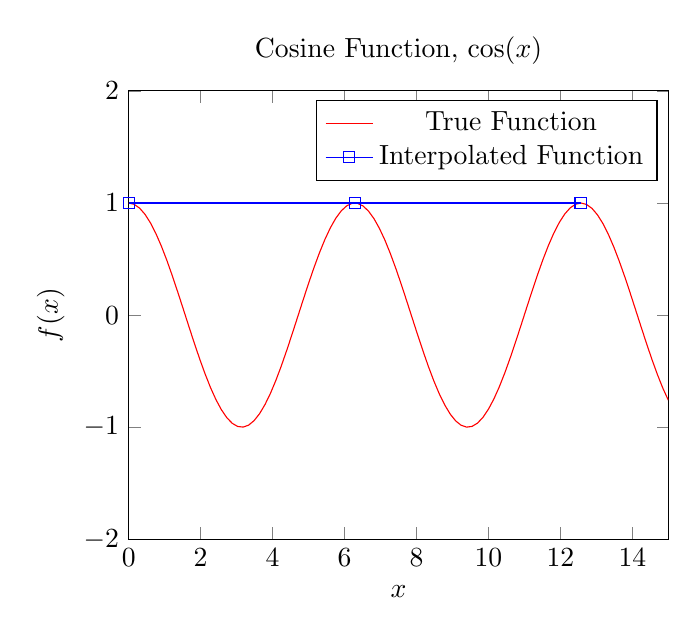
\begin{tikzpicture}
\begin{axis}[
title={Cosine Function, $\cos(x)$},
    xlabel={$x$},
    ylabel={$f(x)$},
    xmin=0, xmax=15, 
    ymin=-2, ymax=2]
\addplot[color=red, domain=0:15, samples=100]{cos(180*x/pi)};
\addlegendentry{True Function}
\addplot[
    color=blue,
    mark=square,
    ]
    coordinates {
    (0,1) (6.28, 1) (12.56, 1)
    };
\addlegendentry{Interpolated Function}
\end{axis}
\end{tikzpicture}
\captionof{figure}{Sampling only once per period provides us with a constant interpolated function, from which we cannot recover the original.  Therefore, we must sample at a higher frequency.}
\end{center}
Note that this holds at points not on the peaks as well:
\begin{center}
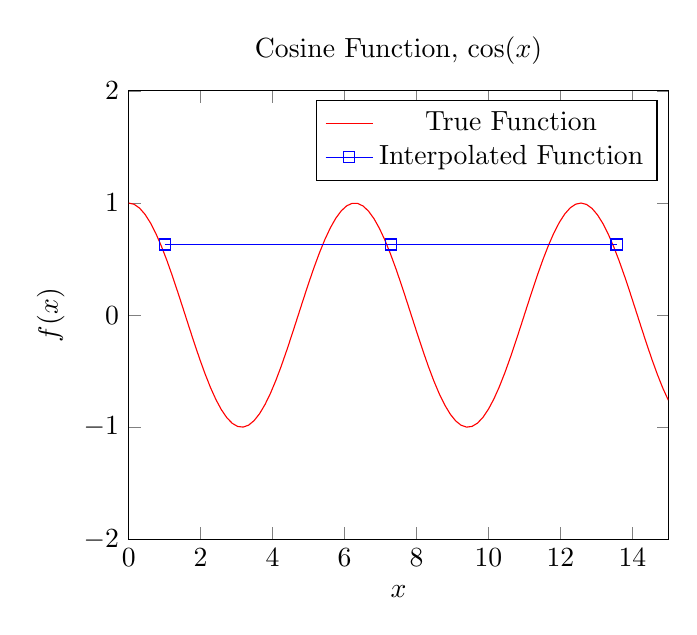
\begin{tikzpicture}
\begin{axis}[
title={Cosine Function, $\cos(x)$},
    xlabel={$x$},
    ylabel={$f(x)$},
    xmin=0, xmax=15, 
    ymin=-2, ymax=2]
\addplot[color=red, domain=0:15, samples=100]{cos(180*x/pi)};
\addlegendentry{True Function}
\addplot[
    color=blue,
    mark=square,
    ]
    coordinates {
    (1,0.63) (7.28, 0.63) (13.56, 0.63)
    };
\addlegendentry{Interpolated Function}
\end{axis}
\end{tikzpicture}
\captionof{figure}{Sampling only once per period provides us with a constant interpolated function, from which we cannot recover the original.  Therefore, we must sample at a higher frequency.}
\end{center}
What if we sample at twice the frequency?  I.e. peaks and troughs:
\begin{center}
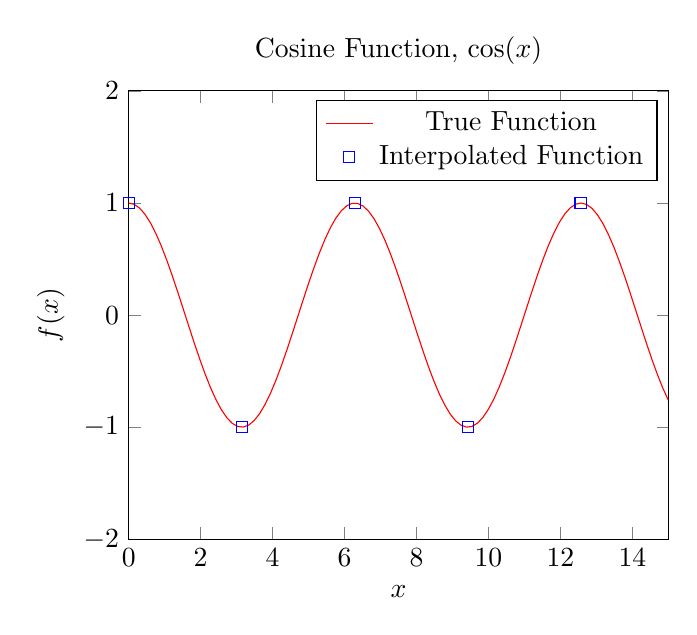
\begin{tikzpicture}
\begin{axis}[
title={Cosine Function, $\cos(x)$},
    xlabel={$x$},
    ylabel={$f(x)$},
    xmin=0, xmax=15, 
    ymin=-2, ymax=2]
\addplot[color=red, domain=0:15, samples=100]{cos(180*x/pi)};
\addlegendentry{True Function}
\addplot[
    only marks,
    color=blue,
    mark=square,
    ]
    coordinates {
    (0,1) (6.28, 1) (12.56, 1) (3.14, -1) (9.42, -1)
    };
\addlegendentry{Interpolated Function}
\end{axis}
\end{tikzpicture}
\captionof{figure}{Sampling at twice the rate as the highest-varying component almost gets us there!  This is known as the \textbf{Nyquist Rate}.  It turns out we need to sample at frequencies that are strictly greater than this frequency to guarantee no aliasing - we will see why in the example below.}
\end{center}
Is this good enough?  As it turns out, the inequality for Nyquist's Sampling Theorem is there for a reason: we need to sample at \textbf{greater than} twice the frequency of the original signal in order to uniquely recover it:
\begin{center}
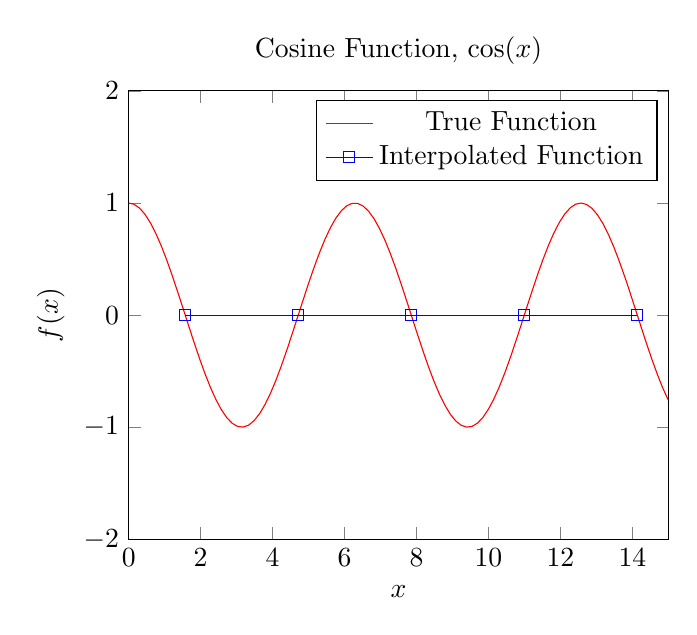
\begin{tikzpicture}
\begin{axis}[
title={Cosine Function, $\cos(x)$},
    xlabel={$x$},
    ylabel={$f(x)$},
    xmin=0, xmax=15, 
    ymin=-2, ymax=2]
\addplot[color=red, domain=0:15, samples=100]{cos(180*x/pi)};
\addlegendentry{True Function}
\addplot[
    color=blue,
    mark=square,
    ]
    coordinates {
    (1.57, 0) (4.71, 0) (7.85, 0) (10.99, 0) (14.13, 0)
    };
\addlegendentry{Interpolated Function}
\end{axis}
\end{tikzpicture}
\captionof{figure}{It turns out we need to sample at frequencies that are strictly greater than this frequency to guarantee no aliasing - we will see why in the example below.}
\end{center}
Therefore, any rate above 2 times the highest-varying frequency component of the signal will be sufficient to completely avoid aliasing.  As a review, let us next discuss aliasing.
\subsubsection{Aliasing}
Aliasing occurs when higher frequencies become indistinguishable from lower frequencies, and as a result they add interference and artifacts to the signal that are caused by sampling at too low of a frequency. \\ \\
Suppose we have a signal given by:
\begin{align*}
    f(x) = \cos(2\pi f_0x) &&
\end{align*}
And suppose we sample this signal with frequency given by $f_s = \frac{1}{\delta}$.  Then our sampled signal is given by:
\begin{align*}
    s_k = \cos(2\pi f_0 k \frac{1}{\delta}) = \cos(2\pi \frac{f_0}{f_s}k) \fa k \in \{1, 2, ...\} &&
\end{align*}
Now let us consider what happens when we add multiples of $2\pi$ to this:
\begin{align*}
    s_{k - 2\pi} & = \cos\Big(2\pi\frac{f_0}{f_s}k - 2\pi k\Big) \\
                 & = \cos\Big(2\pi\Big(\frac{f_0}{f_s} - 1\Big)k\Big) \\
                 & = \cos\Big(2\pi\Big(\frac{f_0-f_s}{f_s}\Big)k\Big) \\
                 & = \cos\Big(2\pi\Big(\frac{f_s-f_0}{f_s}\Big)k\Big), \;\; \text{since} \; \cos(x) = \cos(-x) \fa x \in \R&&
\end{align*}
Another way to put this - you cannot distinguish multiples of base frequencies with the base frequencies themselves if you sample at too low a frequency, i.e. below the \textbf{Nyquist Rate}.
\subsubsection{How Can We Mitigate Aliasing?}
There are several strategies to mitigate aliasing effects:
\begin{itemize}
    \item (Note) Anti-aliasing measures must be taken before sampling.  After sampling occurs, information is ``lost", so to speak, and the original signal cannot be recovered.
    \item High frequency noise suppression with (approximate) low-pass filtering.  As it turns out, exact lowpass filtering is impossible due to convergence properties of Fourier Series at cutoff frequencies (a phenomenon known as the \textbf{Gibbs Phenomenon} [1].
\end{itemize}
We will touch more on these anti-aliasing techniques and strategies throughout this lecture.
\subsection{Integral Image}
Next, we will shift gears somewhat to discuss the notion of an \textbf{integral image}, and the critical role this technique plays in improving computational efficiency in image processing and machine vision. We will disucss this concept in both 1D and 2D.
\subsubsection{Integral Images in 1D}
\textbf{Block averaging} is a common operation in computer vision in which we take the average over a set of values across an entire vector (1D) or matrix (2D), such as an image.  This involves summing and then dividing by the total number of elements, which can become prohibitively computationally-expensive, particularly if this operation is being called many times and the averages that we need to compute are very large.  Is there a more computationally-efficient way to do this?  \\ \\
It turns out this computationally-simpler solution is through integral images.  An integral image is essentially the sum of values from the first value to the $\ith$ value, i.e if $g_i$ defines the $\ith$ value in 1D, then:
\begin{align*}
    G_i \delteq \sum_{k=1}^{i}g_k \fa i \in \{1, \cdots, K\} &&
\end{align*}
Why is this useful?  Well, rather than compute averages (normalized sums) by adding up all the pixels and then dividing, we simply need to perform a single subtraction between the integral image values (followed by a division by the number of elements we are averaging).  For instance, if we wanted to calculate the average of values between $i$ and $j$, then:
\begin{align*}
    \bar{g}_{[i,j]} = \frac{1}{j-i}\sum_{k=i}^{j}g_k = \frac{1}{j-i}(G_j - G_i) &&
\end{align*}
This greatly reduces the amortized amount of computation, because these sums only need to be computed once, when we calculate the initial values for the integral image.
\subsubsection{Integral Images in 2D}
Now, we can extend the notion of an integral image to 2D!  Note further that integral ``images" can extend beyond images!  E.g. these can be done with gradients, Jacobians, Hessians, etc. One example in particular is calculating a Histogram of Gradients (HoG), which is quite useful for feature matching algorithms such as Scale-Invariant Feature Transform (SIFT).   These approaches also map nicely onto GPUs, enabling for even faster computation times.  \\ \\
Let us now see how block averaging looks in 2D - in the diagram below, we can obtain a block average for a group of pixels in the 2D range $(i,j)$ in $x$ and $(k,l)$ in $y$ using the following formula:
\begin{align*}
    \bar{g}_{([i,j], [k,l])} = \frac{1}{(j-i)(l-k)}\sum_{x=i}^{j}\sum_{y=k}^{l}g_{x,y} &&
\end{align*}
But can we implement this more efficiently?  We can use integral images again:
\begin{align*}
    G_{i,j} = \sum_{k=1}^{i}\sum_{l=1}^{j}g_{k,l} &&
\end{align*}
Referencing the figure below, this becomes:
\begin{figure}[H]
    \centering
    \includegraphics[width=2\textwidth/3]{figures/2d_block_averaging.png}
    \caption{Block averaging using integral images in 2D.  As pointed out above, block averaging also extends beyond pixels!  This can be computed for other measures such as gradients (e.g. Histogram of Gradients).}
    \label{fig:my_label}
\end{figure}

Using the integral image values, the block average in the 2D range $(i,j)$ in $x$ and $(k,l)$ in $y$ becomes:
\begin{align*}
    \bar{g}_{([i,j], [k,l])} = \frac{1}{(j-i)(l-k)}\Big((G_{j,l} + G_{i,k}) - (G_{i,l} + G_{j,k})\Big) && 
\end{align*}
Some comments about this:
\begin{itemize}
    \item This analysis can be extended to higher dimensions as well!  Though the integral image will take longer to compute, and the equations for computing these block averages become less intuitive, this approach generalizes to arbitrary dimensions.
    \item As we saw in the one-dimensional case, here we can also observe that after computing the integral image (a one-time operation that can be amortized), the computational cost for averaging each of these 2D blocks becomes \textbf{independent of the size of the block being averaged}.  This stands in stark contrast to the naive implementation - here, the computational cost scales quadratically with the size of the block being averaged (or linearly in each dimension, if we take rectangular block averages).
    \item Why is this relevant?  Recall that block averaging implements approximate lowpass filtering, which can be used as a frequency suppression mechanism to avoid aliasing when filtering.
    \item In other domains outside of image processing, the integral image is known as the ``Summed-area Table" [2].
\end{itemize}
Since we intend to use this for approximate lowpass filtering, let us now change topics toward fourier analysis of this averaging mechanism to see how efficacious it is.
\subsection{Fourier Analysis of Block Averaging}
Let us consider a one-dimensional ``filter" that implements an approximate lowpass filtering for  mechanism through block averaging.  Let us consider a function such that it takes 0 value outside of the range $(-\frac{-\delta}{2}, \frac{\delta}{2})$, and value $\frac{1}{\delta}$ inside this range:
\begin{align*}
    h(x) = \begin{cases}
            \frac{1}{\delta} & x \in (-\frac{-\delta}{2}, \frac{\delta}{2}) \\
            0 & \text{o.w.}
           \end{cases}
\end{align*}
Visually:
\begin{center}
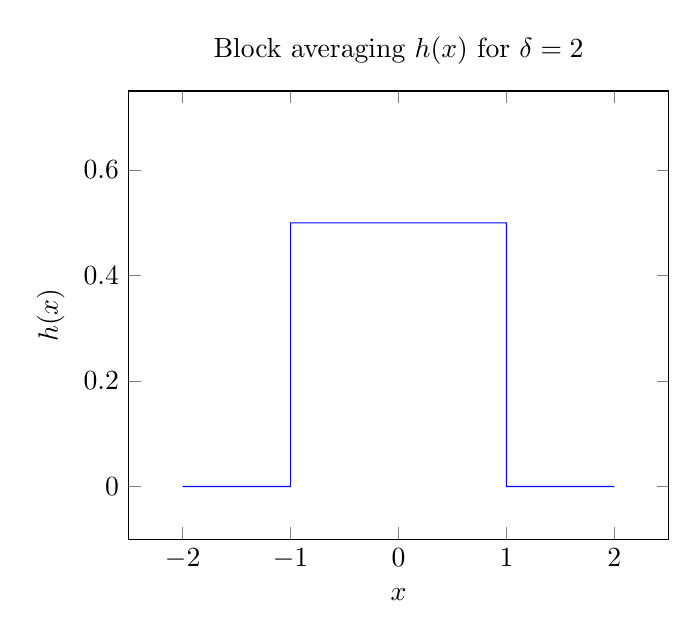
\begin{tikzpicture}
\begin{axis}[
title={Block averaging $h(x)$ for $\delta = 2$},
    xlabel={$x$},
    ylabel={$h(x)$},
    xmin=-2.5, xmax=2.5, 
    ymin=-0.1, ymax=0.75]
\addplot[
    color=blue,
    mark=none,
    ]
    coordinates {
    (-2, 0) (-1.000001, 0) (-1, 1/2) (0, 1/2) (1, 1/2) (1.0000001, 0) (2, 0)
    };
\end{axis}
\end{tikzpicture}
\captionof{figure}{Example $h(x)$ for $\delta = 2$.}
\end{center}
Let's see what this Fourier Transform looks like.  Recall that the Fourier Transform (up to a constant scale factor, which varies by domain) is given by:
\begin{align*}
    F(j\omega) = \int_{-\infty}^{\infty}f(x)e^{-j\omega x}dx &&
\end{align*}
Where $j\omega$ corresponds to complex frequency.  Substituting our expression into this transform:
\begin{align*}
    H(j\omega) & = \int_{-\infty}^{\infty}h(x)e^{-j\omega x}dx \\ \\
               & = \int_{-\frac{\delta}{2}}^{\frac{\delta}{2}}\frac{1}{\delta}e^{-j\omega x}dx \\ \\
               & = \frac{1}{\delta}\frac{1}{j\omega}[e^{-j\omega x}]_{x=-\frac{\delta}{2}}^{x=\frac{\delta}{2}} \\ \\
               & = \frac{e^{-\frac{j\omega\delta}{2}} - e^{\frac{j\omega\delta}{2}}}{-j\omega\delta} \\ \\
               & = \frac{\sin\Big(\frac{\delta\omega}{2}\Big)}{\frac{\delta\omega}{2}} \;\;\textbf{(Sinc function)}
\end{align*}
Where in the last equality statement we use the identity given by:
\begin{align*}
    \sin(x) = \frac{e^{jx}-e^{-jx}}{-2j}
\end{align*}
Graphically, this sinc function appears (for $\delta=2$):
\begin{center}
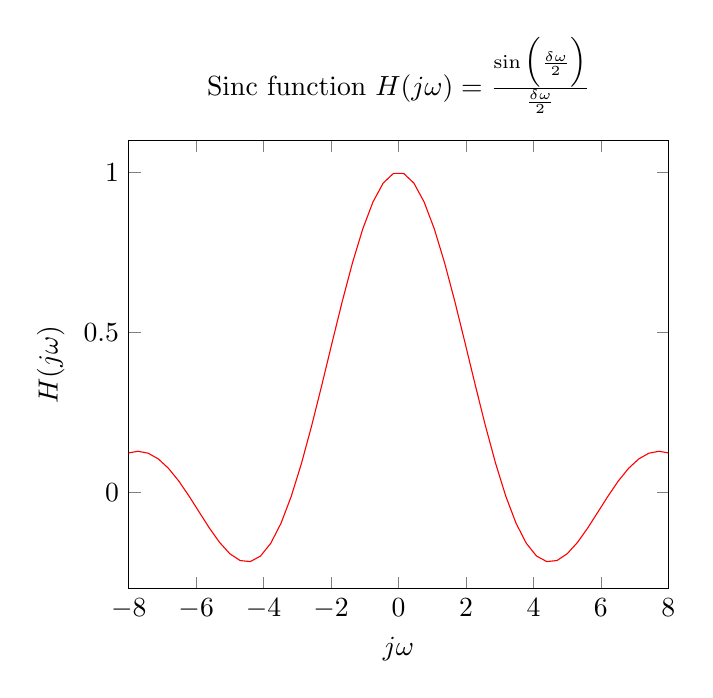
\begin{tikzpicture}
\begin{axis}[
title={Sinc function $H(j\omega) = \frac{\sin\Big(\frac{\delta\omega}{2}\Big)}{\frac{\delta\omega}{2}}$},
    xlabel={$j\omega$},
    ylabel={$H(j\omega)$},
    xmin=-8, xmax=8, 
    ymin=-0.3, ymax=1.1]
\addplot[color=red, domain=-15:15, samples=100]{sin(180*x/pi)/x};
\end{axis}
\end{tikzpicture}
\captionof{figure}{Example $H(j\omega)$ for $\delta = 2$.  This is the Fourier Transform of our block averaging ``filter".}
\end{center}
Although sinc functions in the frequency domain help to attenuate higher frequencies, they do not make the best lowpass filters.  This is the case because:
\begin{itemize}
    \item Higher frequencies are not completely attenuated.
    \item The first zero is not reached quickly enough.  The first zero is given by:
    \begin{align*}
        \frac{\omega_0\delta}{2} = \frac{\pi}{2} \implies \omega_0 = \frac{\pi}{\delta}
    \end{align*}
\end{itemize}
Intuitively, the best lowpass filters perfectly preserve all frequencies up to the cutoff frequencies, and perfectly attenuate everything outside of the passband.  Visually:
\begin{center}
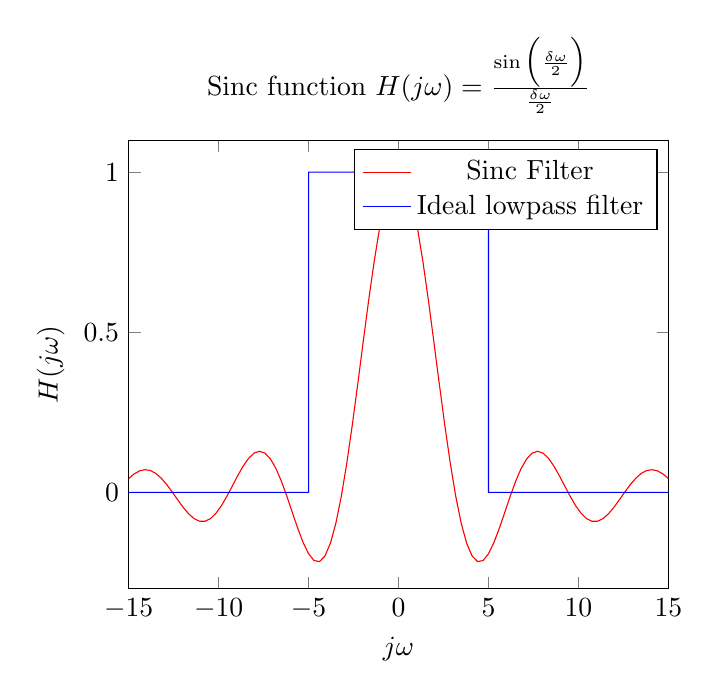
\begin{tikzpicture}
\begin{axis}[
title={Sinc function $H(j\omega) = \frac{\sin\Big(\frac{\delta\omega}{2}\Big)}{\frac{\delta\omega}{2}}$},
    xlabel={$j\omega$},
    ylabel={$H(j\omega)$},
    xmin=-15, xmax=15, 
    ymin=-0.3, ymax=1.1]
\addplot[color=red, domain=-15:15, samples=100]{sin(180*x/pi)/x};
\addlegendentry{Sinc Filter}
\addplot[
    color=blue,
    mark=none,
    ]
    coordinates {
    (-15, 0) (-5.000001, 0) (-5, 1) (0, 1) (5, 1) (5.0000001, 0) (15, 0)
    };
\addlegendentry{Ideal lowpass filter}
\end{axis}
\end{tikzpicture}
\captionof{figure}{Frequency response comparison between our block averaging filter and an ideal lowpass filter.  We also note that the ``boxcar" function and the sinc function are Fourier Transform pairs!}
\end{center}
Although sinc functions in the frequency domain help to attenuate higher frequencies, they do not make the best lowpass filters.  This is the case because:
\begin{itemize}
    \item Higher frequencies are not completely attenuated.
    \item The first zero is not reached quickly enough.  The first zero is given by:
    \begin{align*}
        \frac{\omega_0\delta}{2} = \frac{\pi}{2} \implies \omega_0 = \frac{\pi}{\delta}
    \end{align*}
\end{itemize}
Where else might we see this?  It turns out cameras perform block average filtering because pixels have finite width over which to detect incident photons.  But is this a sufficient approximate lowpass filtering technique?  Unfortunately, oftentimes it is not.  We will see below that we can improve with \textbf{repeated block averaging}.
\subsection{Repeated Block Averaging}
One way we can improve our ability to attenuate higher frequencies - repeated block averaging!  If our ``boxcar" filter given above is given by $b(x)$ (note that this was $h(x)$ above), then our previous result $y(x)$ can be written as:
\begin{align*}
    y_1(x) = f(x) \otimes b(x)
\end{align*}
\begin{center}
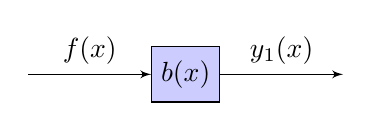
\begin{tikzpicture}[node distance=2.5cm,auto,>=latex']
    \node [int] (a) {$b(x)$};
    \node (b) [left of=a,node distance=2cm, coordinate] {a};
    \node [coordinate] (end) [right of=a, node distance=2cm]{};
    \path[->] (b) edge node {$f(x)$} (a);
    \draw[->] (a) edge node {$y_1(x)$} (end) ;
\end{tikzpicture}
\end{center}
What happens if we add another filter?  Then, we simply add another element to our convolution:
\begin{align*}
    y_2(x) = (f(x) \otimes b(x)) \otimes b(x) = y_1(x) \otimes b(x)
\end{align*}
\begin{center}
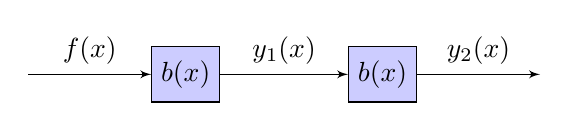
\begin{tikzpicture}[node distance=2.5cm,auto,>=latex']
    \node [int] (a) {$b(x)$};
    \node (b) [left of=a,node distance=2cm, coordinate] {a};
    \node [int] (c) [right of=a] {$b(x)$};
    \node [coordinate] (end) [right of=c, node distance=2cm]{};
    \path[->] (b) edge node {$f(x)$} (a);
    \path[->] (a) edge node {$y_1(x)$} (c);
    \draw[->] (c) edge node {$y_2(x)$} (end) ;
\end{tikzpicture}
\end{center}
Adding this second filter is equivalent to convolving our signal with the convolution of two ``boxcar" filters, which is a triangular filter:
\begin{center}
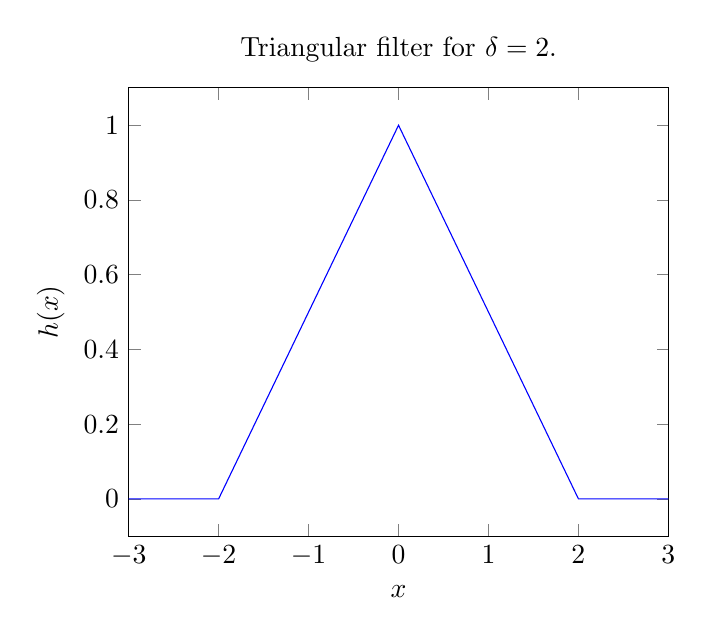
\begin{tikzpicture}
\begin{axis}[
title={Triangular filter for $\delta = 2$.},
    xlabel={$x$},
    ylabel={$h(x)$},
    xmin=-3, xmax=3, 
    ymin=-0.1, ymax=1.1]
\addplot[
    color=blue,
    mark=none,
    ]
    coordinates {
    (-3, 0) (-2, 0) (0, 1) (2, 0) (3, 0)
    };
\end{axis}
\end{tikzpicture}
\captionof{figure}{Example of a triangular filter resulting from the convolution of two ``boxcar" filters.}
\end{center}
Additionally, note that since convolution is associative, for the ``two-stage" approximate lowpass filtering approach above, we do not need to convolve our input $f(x)$ with two ``boxcar" filters - rather, we can convolve it directly with our trinagular filter $b_2(x) = b(x) \otimes b(x)$:
\begin{align*}
    y_2(x) & = (f(x) \otimes b(x)) \otimes b(x) \\
           & = f(x) \otimes (b(x) \otimes b(x)) \\
           & = f(x) \otimes b_2(x)
\end{align*}
Let us now take a brief aside to list out how discontinuities affect Fourier Transforms in the frequency domains:
\begin{itemize}
    \item \textbf{Delta Function}: $\delta(x) \ftpair 1$ \\ \\
    \textbf{Intuition}: Convolving a function with a delta function does not affect the transform, since this convolution simply produces the function.
    \item \textbf{Unit Step Function}: $u(x) \ftpair \frac{1}{j\omega}$ \\ \\
    \textbf{Intuition}: Convolving a function with a step function produces a degree of averaging, reducing the high frequency components and therefore weighting them less heavily in the transform domain.
    \item \textbf{Ramp Function}: $r(x) \ftpair -\frac{1}{\omega^2}$ \\ \\
    \textbf{Intuition}: Convolving a function with a ramp function produces a degree of averaging, reducing the high frequency components and therefore weighting them less heavily in the transform domain.
    \textbf{Derivative}: $\frac{d}{dx}f(x) \ftpair j\omega F(j\omega)$ \\ \\
    \textbf{Intuition}: Since taking derivatives will increase the sharpness of our functions, and perhaps even create discontinuities, a derivative in the spatial domain corresponds to multiplying by $j\omega$ in the frequency domain.  
\end{itemize}
As we can see from above, the more ``averaging" effects we have, the more the high-frequency components of the signal will be filtered out.  Conversely, when we take derivatives and create discontinuities in our spatial domain signal, this increases high frequency components of the signal because it introduces more variation. \\ \\
To understand how we can use repeated block averaging in the Fourier domain, please recall the following special properties of Fourier Transforms:
\begin{enumerate}
     \item \textbf{Convolution in the spatial domain corresponds to multiplication in the frequency domain}, i.e. for all $f(x), g(x), h(x)$ with corresponding Fourier Transforms $F(j\omega), G(j\omega), H(j\omega)$, we have:
    \begin{align*}
        h(x) = f(x) \otimes g(x) \ftpair H(j\omega) = F(j\omega)G(j\omega)
    \end{align*}
    \item \textbf{Multiplication in the spatial domain corresponds to convolution in the frequency domain}, i.e. for all $f(x), g(x), h(x)$ with corresponding Fourier Transforms $F(j\omega), G(j\omega), H(j\omega)$, we have:
    \begin{align*}
        h(x) = f(x)g(x) \ftpair H(j\omega) = F(j\omega) \otimes G(j\omega)
    \end{align*}
\end{enumerate}
For block averaging, we can use the first of these properties to understand what is happening in the frequency domain:
\begin{align*}
    y_2(x) = f(x) \otimes (b(x) \otimes b(x)) \ftpair Y(j\omega) = F(j\omega)(B(j\omega)^2)
\end{align*}
This operation is equivalent to a $\text{sinc}^2$ function in the spatial domain:
\begin{center}
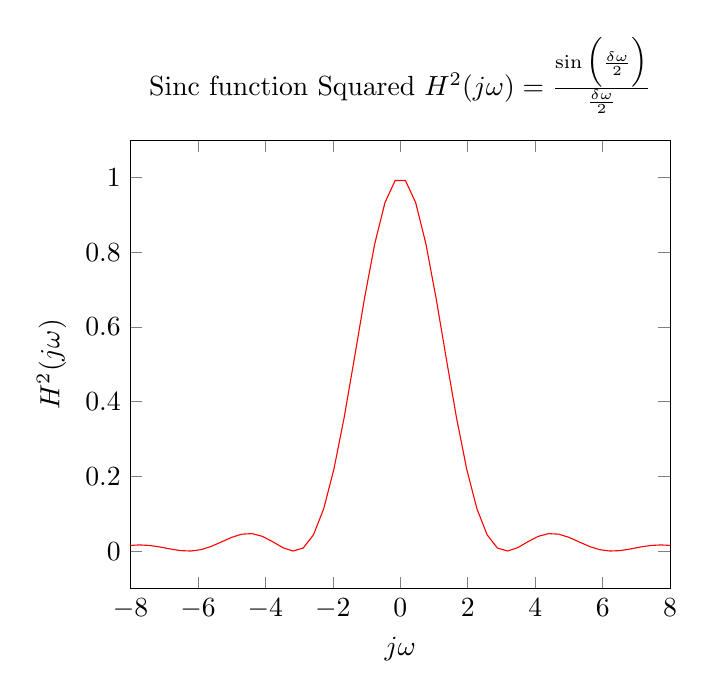
\begin{tikzpicture}
\begin{axis}[
title={Sinc function Squared $H^2(j\omega) = \frac{\sin\Big(\frac{\delta\omega}{2}\Big)}{\frac{\delta\omega}{2}}$},
    xlabel={$j\omega$},
    ylabel={$H^2(j\omega)$},
    xmin=-8, xmax=8, 
    ymin=-0.1, ymax=1.1]
\addplot[color=red, domain=-15:15, samples=100]{(sin(180*x/pi)/x)^2};
\end{axis}
\end{tikzpicture}
\captionof{figure}{Example $H^2(j\omega)$ for $\delta = 2$.  This is the Fourier Transform of our block averaging ``filter" convolved with itself in the spatial domain.}.
\end{center}
This is not perfect, but it is an improvement.  In fact, the frequencies with this filter drop off with magnitude $\Big(\frac{1}{\omega})^2$.  What happens if we continue to repeat this process with more block averaging filters?  It turns out that for $N$ ``boxcar" filters that we use, the magnitude will drop off as $\Big(\frac{1}{\omega}\Big)^N$.  Note too, that we do not want to go ``too far" in this direction, because this repeated block averaging process will also begin to attenuate frequencies in the passband of the signal.
\subsubsection{Warping Effects and Numerical Fourier Transforms: FFT and DFT}
Two main types of numerical transforms we briefly discuss are the Discrete Fourier Transform (DFT) and Fast Fourier Transform (FFT).  The FFT is an extension of the DFT that relies on using a ``divide and conquer" approach to reduce the computational runtime from $f(N) \in O(N^2)$ to $f(N) \in O(N\log N)$ [3]. \\ \\
Mathematically, the DFT is given as a transform that transforms a sequence of $N$ complex numbers $\{x_n\}_{n=1}^{N}$ into another sequence of $N$ complex numbers $\{X_k\}_{k=1}^{N}$ [4].  The transform for the $K^{\text{th}}$ value of this output sequence is given in closed-form as:
\begin{align*}
    X_k = \sum_{i=1}^{N}x_ne^{-j\frac{2\pi}{N}kn}
\end{align*}
And the inverse transform for the $n^{\text{th}}$ value of this input sequence is given as:
\begin{align*}
    x_n = \sum_{k=1}^{N}X_ke^{j\frac{2\pi}{N}kn}
\end{align*}
One aspect of these transforms to be especially mindful of is that they introduce a wrapping effect, since transform values are spread out over 2$\pi$ intervals.  This means that the waveforms produced by these transforms, in both the spatial (if we take the inverse transform) and frequency domains may be repeated - this repeating can introduce undesirable discontinuities, such as those seen in the graph below:
\begin{center}
\begin{tikzpicture}
\begin{axis}[
title={Repeated Function $x^2$},
    xlabel={$x$},
    ylabel={$f(x)$},
    xmin=0, xmax=8, 
    ymin=0, ymax=8]
\addplot[color=red, domain=0:2.5, samples=100]{x^2};
\addplot[color=red, domain=2.5:5.0, samples=100]{(x-2.5)^2};
\addplot[color=red, domain=5.0:7.5, samples=100]{(x-5.0)^2};
\end{axis}
\end{tikzpicture}
\captionof{figure}{Example of a repeated waveform that we encounter when looking at DFTs and FFTs.}
\end{center}
\textbf{Fun fact}: It used to be thought that natural images had a power spectrum (power in the frequency domain) that falls off as $\frac{1}{\omega}$.  It turns out that this was actually caused by warping effects introduced by discrete transforms. \\ \\
This begs the question - how can we mitigate these warping effects?  Some methods include:
\begin{itemize}
    \item \textbf{Apodizing}: This corresponds to multiplying your signal by a waveform, e.g. Hamming's Window, which takes the form akin to a Gaussian, or an inverted cosine.
    \item \textbf{Mirroring}: Another method to mitigate these warping effects is through waveform mirroring - this ensures continuity at points where discontinuties occurred:
    \begin{center}
    \begin{tikzpicture}
    \begin{axis}[
    title={Repeated Function $x^2$},
        xlabel={$x$},
        ylabel={$f(x)$},
        xmin=0, xmax=8, 
        ymin=0, ymax=8]
    \addplot[color=red, domain=0:2.5, samples=100]{x^2};
    \addplot[color=red, domain=2.5:5.0, samples=100]{(2.5-(x-2.5))^2};
    \addplot[color=red, domain=5.0:7.5, samples=100]{(x-5.0)^2};
    \end{axis}
    \end{tikzpicture}
    \captionof{figure}{Example of a mirrored waveform that we can use to counter and mitigate the discontinuity effects of warping from transforms such as the DFT and FFT.}
    \end{center}
    With this approach, the power spectrum of these signals falls off at $\frac{1}{\omega^2}$, rather than $\frac{1}{\omega}$.
    \item \textbf{Infinitely Wide Signal}: Finally, a less practical, but conceptual helpful method is simply to take an ``infinitely wide signal".
\end{itemize}
Let us now switch gears to talk more about the unit impulse and convolution.
\subsection{Impulses and Convolution}
In this section, we will review impulse functions, and discuss how they relate to many properties with convolution.  We will begin by reviewing delta functions and their properties.
\subsubsection{Properties of Delta Functions}
Recall that the Dirac delta function $\delta(x)$, or impulse function, is defined according to the two properties:
\begin{enumerate}
    \item \textbf{Unit Area}: $\int_{-\infty}^{\infty}\delta(x)dx = 1$
    \item \textbf{Sifting Property}: $f(x_0) = \int_{-\infty}^{\infty}f(x)\delta(x-x_0)dx$
\end{enumerate}
Another way to conceptualize delta functions is through \textbf{probabilistic distributions}.  We can use Gaussians (one of the only distributions to have a Fourier Transform).  Recall that the (zero-mean) Gaussian Fourier Transform pair is given by:
\begin{align*}
    \frac{1}{\sigma\sqrt{2\pi}}e^{-\frac{x}{2\sigma^2}} \ftpair e^{-\frac{\omega^2\sigma^2}{2}}
\end{align*}
An impulse can be conceptualized as the limit in which the variance of this Gaussian distribution $\sigma^2$ goes to 0, which corresponds to a Fourier Transform of 1 for all frequencies (which is the Fourier Transform of a delta function). \\ \\
Another way to consider impulses is that they are the limit of ``boxcar" functions as their width goes to zero. \\ \\
Let us next generalize from a single impulse function to combinations of these functions.
\subsubsection{Combinations of Impulses}
When are combinations of impulses helpful?  it turns out that one particular combination can be used for approximating the derivative using our prior work on finite differences:
\begin{align*}
    h(x) = \frac{1}{\epsilon}\Big(\delta(x + \frac{\epsilon}{2}) - \delta(x-\frac{\epsilon}{2})\Big) \;\; \text{for some} \; \epsilon > 0
\end{align*}
Correlating (*note that this is not convolution - if we were to use convolution, this derivative would be flipped) this combination of impulse ``filter" with an arbitrary function $f(x)$, we compute a first-order approximation of the derivative:
\begin{align*}
    f'(x) & \approx \int_{-\infty}^{\infty}f(x)h(x)dx \\
          & = \int_{-\infty}^{\infty}\Big(\frac{1}{\epsilon}\Big(\delta(x + \frac{\epsilon}{2}) - \delta(x-\frac{\epsilon}{2})\Big)\Big)dx
\end{align*}
Therefore, combinations of impulses can be used to represent the same behavior as the ``computational molecules" we identified before.  It turns out that there is a close connection between \textbf{linear, shift-invariant} operators and \textbf{derivative operators}. \\ \\
With impulses motivated, let us now formally review convolution.
\subsubsection{Convolution Review}
Recall from the example above that the convolution operation is simply the result of the correlation operation flipped.  Mathematically, the convolution of functions $f(x)$ and $h(x)$ is given by the following commutative operation:
\begin{align*}
    g(x) & = f(x) \otimes h(x) \\
         & = \int_{-\infty}^{\infty}f(\xi)h(x-\xi)d\xi \\
         & = h(x) \otimes g(x) \\
         & = \int_{-\infty}^{\infty}h(\xi)f(x-\xi)d\xi \\
\end{align*}
\subsubsection{Analog Filtering with Birefringent Lenses}
Why filter in the analog domain?  Returning to our original problem of mitigating aliasing artifacts through high-frequency suppression, unfortunately, if we wait to digitally filter out high frequencies after the image has already been taken by a camera or sensor, then we have already caused aliasing. \\ \\
One way to achieve this analog filtering is through \textbf{Birefringent Lenses}.  Here, we essentially take two ``shifted" images by convolving the image with a symmetric combination of offset delta functions, given mathematically by:
\begin{align*}
    h(x) = \frac{1}{2}\delta(x + \frac{\epsilon}{2}) + \frac{1}{2}\delta(x - \frac{\epsilon}{2}) \;\; \text{for some} \;\epsilon > 0
\end{align*}
Let us look at the Fourier Transform of this filter, noting the following Fourier Transform pair:
\begin{align*}
    \delta(x-x_0) \ftpair e^{-j\omega x_0}
\end{align*}
With this we can then express the Fourier Transform of this filter as:
\begin{align*}
    F(j\omega) & = \frac{1}{\sqrt{2\pi}}\int_{-\infty}^{\infty}h(x)e^{-j\omega x}dx \\
               & = \frac{1}{2}\Big(e^{-\frac{j\omega\epsilon}{2}} + e^{\frac{j\omega\epsilon}{2}}\Big) \\
               & = \cos\Big(\frac{\omega\epsilon}{2}\Big)
\end{align*}
With this framework, the first zero to appear here occurs at $\omega_0 = \frac{\pi}{\epsilon}$.  A few notes about these filters, and how they relate to high-frequency noise suppression.
\begin{itemize}
    \item When these birefringent lenses are cascaded with a \textbf{block averaging} filter, this results in a combined filtering scheme in which the zeros of the frequency responses of these filters cancel out most of the high-frequency noise.
    \item In the 2D case, we will have 2 birefringent filters, one for the x-direction and one for the y-direction.  Physically, these are rotated 90 degrees off from one another, just as they are for a 2D cartesian coordinate system.
    \item High-performance lowpass filtering requires a large \textbf{support} (see definition of this below if needed) - the computational costs grow linearly with the size of the support in 1D, and quadratically with the size of the support in 2D.  The support of a function is defined as the set where $f(\cdot)$ is nonzero [5]:
    \begin{align*}
        \text{supp}(f) = \{x: f(x) \neq 0, x \in \mathbb{R}\}
    \end{align*}
    \item Therefore, one way to reduce the computatonal costs of a filtering system is to reduce the size/cardinality of the support $|\text{supp}(f)|$ - in some sense to encourage sparsity.  Fortunately, this does not necessarily mean looking over a narrower range, but instead just considering less points overall.
\end{itemize}
\subsubsection{Derivatives and Integrals as Convolution Operators and FT Pairs}
As we have seen before, convolving a function with a unit step function results in integrating the given function.  Let us verify this below:
\begin{align*}
    f(x) \otimes u(x) & = \int_{-\infty}^{\infty}f(\xi)u(x-\xi)d\xi \\
                      & = \int_{-\infty}^{\infty}f(x-\xi)u(\xi)d\xi \\
                      & = \int_{0}^{\infty}f(\xi)d\xi
\end{align*}
Therefore, we can represent integral and derivative operators as Fourier Transform pairs too, denoted $\mathcal{S}$ for integration and $\mathcal{D}$ for derivative:
\begin{itemize}
    \item $\mathcal{S} \ftpair \frac{1}{j\omega}$
    \item $\mathcal{D} \ftpair j\omega$
\end{itemize}
Niote that we can verify this by showing that convolving these filter operators corresponds to multiplying these transforms in frequency space, which results in no effect when cascaded together:
\begin{align*}
    (f(x) \otimes \mathcal{D}) \otimes \mathcal{S} = f(x) \otimes (\mathcal{D} \otimes \mathcal{S}) \ftpair F(j\omega)\Big(j\omega \frac{1}{j\omega}\Big) = F(j\omega) \ftpair f(x)
\end{align*}
\begin{center}
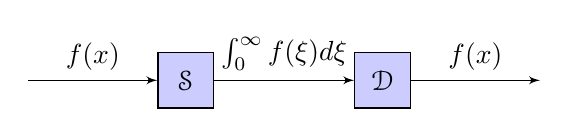
\begin{tikzpicture}[node distance=2.5cm,auto,>=latex']
    \node [int] (a) {$\mathcal{S}$};
    \node (b) [left of=a,node distance=2cm, coordinate] {a};
    \node [int] (c) [right of=a] {$\mathcal{D}$};
    \node [coordinate] (end) [right of=c, node distance=2cm]{};
    \path[->] (b) edge node {$f(x)$} (a);
    \path[->] (a) edge node {$\int_{0}^{\infty}f(\xi)d\xi$} (c);
    \draw[->] (c) edge node {$f(x)$} (end) ;
\end{tikzpicture}
\end{center}
\begin{center}
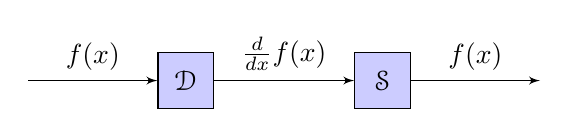
\begin{tikzpicture}[node distance=2.5cm,auto,>=latex']
\node [int] (a) {$\mathcal{D}$};
\node (b) [left of=a,node distance=2cm, coordinate] {a};
\node [int] (c) [right of=a] {$\mathcal{S}$};
\node [coordinate] (end) [right of=c, node distance=2cm]{};
\path[->] (b) edge node {$f(x)$} (a);
\path[->] (a) edge node {$\frac{d}{dx}f(x)$} (c);
\draw[->] (c) edge node {$f(x)$} (end) ;
\end{tikzpicture}
\end{center}
Can we extend this to higher-order derivatives?  It turns out we can.  One example is the convolution of two derivative operators, which becomes:
\begin{align*}
    h(x) = \delta(x+\frac{\epsilon}{2}) - 2\delta(x) + \delta(x -\frac{\epsilon}{2}) = \mathcal{D} \otimes \mathcal{D} \ftpair H(j\omega) = D(j\omega)^2 = (j\omega)^2 = -\omega^2 \;\; \text{(Recall that} \; j^2 = -1)
\end{align*}
In general, this holds.  Note that the number of integral operators $\mathcal{S}$ must be equal to the number of derivative operators $\mathcal{D}$, e.g. for $K\th$ order:
\begin{align*}
    \Big(\otimes_{i=1}^{K}\mathcal{S}\Big) \otimes \Big(\Big(\otimes_{i=1}^{K}\mathcal{D}\Big) \otimes f(x)\Big)
\end{align*}
\subsubsection{Interpolation and Convolution}
A few notes about interpolation methods:
\begin{itemize}
    \item These methods work well computationally when there is sparsity in the operators we with - for instance, cubic or linear interpolation.  Photoshop and other photo-editing software frameworks iuse this interpolation techniques.  Performance deteriorates when we switch from \textbf{cubic interpolation} to \textbf{Nearest Neighbor interpolation}.
    \item The \textbf{bicubic spline} is a popular interpolation technique.  It was invented by IBM and was used in early satellite image processing.  However, it requires many neighboring pixels, as it is composed of 7 points to interpolate over, so it is less computationally-efficient.
    \item Recall that one key element of computational efficiency we pursue is to use integral images for block averaging, which is much more efficient than computing naive sums, especially if (1) This block averaging procedure is repeated many times (the amortized cost of computing the integral image is lessened) and (2) This process is used in higher dimensions.
    \item \textbf{Linear interpolation} can be conceptualized as connecting points together using straight lines between points.  This corresponds to piecewise-linear segments, or, convolution with a triangle filter, which is simply the convolution of two ``boxcar filters":
    \begin{align*}
        f(x) = f(1)x + f(0)(1-x)
    \end{align*}
    Unfortunately, one ``not-so-great" property of convolving with triangular filters for interpolation is that the noise in the interpolated result varies depending on how far away we are from the sampled noise.
    \item \textbf{Nearest Neighbor} techniques can also be viewed through a convolutional lens - since this method produces piecewise-constant interpolation, this is equivalent to convolving our sampled points with a ``boxcar" filter!
\end{itemize}
\subsubsection{Rotationally-Symmetric Lowpass Filter in 2D}
Where $u$ and $v$ are the spatial frequencies of $x$ and $y$, i.e. the 2D Fourier Transform and Inverse Fourier Transform then take the forms of:
\begin{align*}
    & F(u,v) = \frac{1}{\sqrt{2\pi}}\int_{-\infty}^{\infty}\int_{-\infty}^{\infty}f(x,y)e^{-j(ux+vy)}dxdy \\
    & f(x,y) = \frac{1}{\sqrt{2\pi}}\int_{-\infty}^{\infty}\int_{-\infty}^{\infty}F(u,v)e^{j(ux+vy)}dudv \\
\end{align*}
The inverse transform of this can be thought of as a \textbf{sinc} function in polar coordinates:
\begin{align*}
    f(\rho, \theta) = \frac{B^2}{2\pi}\frac{J_1(\rho B)}{\rho B}
\end{align*}
A few notes about this inverse transform function:
\begin{itemize}
    \item This is the point spread function of a microscope.
    \item $J_1(\cdot)$ is a 1st-order Bessel function.
    \item This relates to our \textbf{defocusing} problem that we encountered before.
    \item In the case of defocusing, we can use the ``symmetry" property of the Fourier Transform to deduce that if we have a circular point spread function resulting from defocusing of the lens, then we will have a Bessel function in the frequency/Fourier domain.
    \item Though a pointspread function is a ``pillbox" in the ideal case, in practice this is not perfect due to artifacts such as lens aberrations.
\end{itemize}
\subsection{References}
\begin{enumerate}
    \item Gibbs Phenomenon, https://en.wikipedia.org/wiki/Gibbs\_phenomenon
    \item Summed-area Table, https://en.wikipedia.org/wiki/Summed-area\_table
    \item Fast Fourier Transform, https://en.wikipedia.org/wiki/Fast\_Fourier\_transform
    \item Discrete Fourier Transform, https://en.wikipedia.org/wiki/Discrete\_Fourier\_transform
    \item Support, https://en.wikipedia.org/wiki/Support\_(mathematics)
\end{enumerate}

%%%%%%%%%%%%%%%%%%%%%%%%%%%%% LEC 17 %%%%%%%%%%%%%%%%%%%%%%%%%%%%%%%%%%%%%%%%%%%%%%%%
\section{Lecture 17: Photogrammetry, Orientation, Axes of Inertia, Symmetry, Absolute, Relative, Interior, and Exterior Orientation}
This lecture marks a transition in what we have covered so far in the course from lower-level machine vision to higher-level problems, beginning with photogrammetry. \\ \\
\textbf{Photogrammetry}: ``Measurements from Imagery", for example, map-making.
\subsection{Photogrammetry Problems: An Overview}
Four important problems in photogrammetry that we will cover are:
\begin{itemize}
    \item \textbf{Absolute Orientation} $3D \longleftrightarrow 3D$
    \item \textbf{Relative Orientation} $2D \longleftrightarrow 2D$
    \item \textbf{Exterior Orientation} $2D \longleftrightarrow 3D$
    \item \textbf{Intrinsic Orientation} $3D \longleftrightarrow 2D$
\end{itemize}
Below we discuss each of these problems at a high level.  We will be discussing these problems in greater depth later in this and following lectures.
\subsubsection{Absolute Orientation}
We will start with covering \textbf{absolute orientation}.  This problem asks about the relationship between two or more objects (cameras, points, other sensors) in 3D.  Some examples of this problem include:
\begin{enumerate}
    \item Given two 3D sensors, such as lidar (light detection and ranging) sensors, our goal is to find the \textbf{transformation}, or \textbf{pose}, between these two sensors.
    \item Given one 3D sensor, such as a lidar sensor, and two objects (note that this could be two distinct objects at a single point in time, or a single object at two distinct points in time), our goal is to find the \textbf{transformation}, or \textbf{pose}, between the two objects.
\end{enumerate}
\subsubsection{Relative Orientation}
This problem asks how we can find the 2D $\longleftrightarrow$ 2D relationship between two objects, such as cameras, points, or other sensors.  This type of problem comes up frequently in machine vision, for instance, \textbf{binocular stereo}.  Two high-level applications include:
\begin{enumerate}
    \item Given two cameras/images that these cameras take, our goal is to extract 3D information by finding the relationship between two 2D images.
    \item Given two cameras, our goal is to find the (relative) \textbf{transformation}, or \textbf{pose}, between the two cameras.
\end{enumerate}
\subsubsection{Exterior Orientation}
This photogrammetry problem aims from going 2D $\longrightarrow$ 3D.  One common example in robotics (and other field related to machine vision) is \textbf{localization}, in which a robotic agent must find their location/orientation on a map given 2D information from a camera (as well as, possibly, 3D laser scan measurements). \\ \\
More generally, with \textbf{localization}, our goal is to find where we are and how we are oriented in space given a 2D image and a 3D model of the world.
\subsubsection{Interior Orientation}
This photogrammetry problem aims from going 3D $\longrightarrow$ 2D.  The most common application of this problem is \textbf{camera calibration}.  Camera calibration is crucial for high-precision imaging, as well as solving machine and computer vision problems such as Bundle Adjustment [1].  Finding a principal point is another example of the interior orientation problem.
\subsection{Absolute Orientation}
We will begin our in-depth discussion and analysis of these four problems with \textbf{absolute orientation}.  Let us start by introducing binocular stereo.
\subsubsection{Binocular Stereopsis}
To motivate binocular stereo, we will start with a fun fact: Humans have $\approx$ 12 depth cues.  One of these is \textbf{binocular stereopsis}, or \textbf{binocular stereo} (binocular $\approx$ two sensors). \\ \\
Binocular stereo is given by the figure below:
\begin{figure}[H]
    \centering
    \includegraphics[width=\textwidth]{figures/binocular_stereo.png}
    \caption{The problem of binocular stereo.  Having two 2D sensors enables us to recover 3D structure (specifically, depth) from the scene we image.  A few key terms/technicalities to note here: (i) The origin is set to be halfway between the two cameras, (ii) The distance between the cameras is called the \textbf{baseline}, and (iii) \textbf{binocular disparity} refers to the phenomenon of having each camera generate a different image.  Finally, note that in practice, it is almost impossible to line up these cameras exactly.}
    \label{fig:my_label}
\end{figure}
\textbf{Goal}: Calculate $X$ and $Z$.  This would not be possible with only monocular stereo (monocular $\approx$ one sensor).  Using similar triangles, we have:
\begin{align*}
    & \frac{X - \frac{b}{2}}{Z} = \frac{x_l}{f} \\
    & \frac{X + \frac{b}{2}}{Z} = \frac{x_r}{f} \\
    & \longrightarrow \frac{x_r - x_l}{f} = \frac{b}{z} \implies z = \frac{bf}{x_r - x_l} &&
\end{align*}
Where the \textbf{binocular disparity} is given by $(x_r - x_l)$.  Solving this system of equations becomes:
\begin{align*}
    X = b\frac{x_r + x_l}{x_r - x_l}, \; Z = bf\frac{1}{x_r-x_l} &&
\end{align*}
Note that, more generally, we can calculate in the same way as well!  From these equations, we can see that:
\begin{itemize}
    \item Increasing the baseline increases $X$ and $Z$ (all things equal)
    \item Increasing the focal length increases $Z$.
\end{itemize}
But it is important to also be mindful of system constraints that determine what range, or the exact value, of what these variables can be.  For instance, if we have a self-driving car, we cannot simply have the baseline distance between our two cameras be 100 meters, because this would require mounting the cameras 100 meters apart.
\subsubsection{General Case}
All of the methods we have looked at so far assume we have already found ``interesting points", for instance, through feature detection algorithms (also known as ``descriptors") such as SIFT, SURF, ORB, or FAST+BRIEF.  In the general case, absolute orientation involves having a point in space that is measured by two separate frames of reference (could be a camera, or another sensor), and the goal is to find the \textbf{closest approach} between coordinate systems, a.k.a. the shortest line that connects them.  We will arbitrarily assign the 3 x 3 matrix $(\mb{x}_l, \mb{y}_l, \mb{z}_l) \in \Rd{3 \times 3}$ to refer to a ``lefthanded" coordinate system, and 3 x 3 matrix $(\mb{x}_r, \mb{y}_r, \mb{z}_r) \in \Rd{3 \times 3}$ to refer to a ``righthanded" coordinate system, where our goal is to find the transformation between these two coordinate systems.  The diagram below illustrates this:
\begin{figure}[H]
    \centering
    \includegraphics[width=\linewidth/2]{figures/absolute_orientation.png}
    \caption{General case of absolute orientation: Given the coordinate systems $(\mb{x}_l, \mb{y}_l, \mb{z}_l) \in \Rd{3 \times 3}$ and $(\mb{x}_r, \mb{y}_r, \mb{z}_r) \in \Rd{3 \times 3}$, our goal is to find the transformation, or pose, between them using points measured in each frame of reference $\mb{p}_i$.}
    \label{fig:my_label}
\end{figure}
Here, we also note the following, as they are important for establishing that we are not limited just to finding the transformation between two camera sensors:
\begin{itemize}
    \item ``Two cameras" does not just mean having two distinct cameras (known as ``two-view geometry"); this could also refer to having a single camera with images taken at two distinct points in time (known as ``Visual Odometry" or ``VO").
    \item Note also that we could have the same scenario described above when introducing this problem, which is that we have either one camera and multiple objects, or multiple objects and one cameras.  Hence, there is a sense of duality here with solving these problems:
    \begin{enumerate}
        \item One camera, two objects?
        \item Two cameras, one object (Two-View Geometry)?
        \item Camera moving (VO)?
        \item Object moving?
    \end{enumerate}
\end{itemize}
To better understand this problem, it is first important to precisely define the \textbf{transformation} or \textbf{pose} (translation + rotation) between the two cameras.
\subsubsection{Transformations and Poses}
Recall that in 3D, we have 6 degrees of freedom (DOF), of which \textbf{3} are for \textbf{translation}, and \textbf{3} are for \textbf{rotation}.  In the general case of a $d$-dimensional system, we will have $d$ \textbf{translational} degrees of freedom, and $\frac{d(d-1)}{2}$ \textbf{rotational} degrees of freedom (which, interestingly, is also equal to $\sum_{i=0}^{d-1}i$.  Therefore, for a $d$-dimensional system, the total degrees of freedom from translation and rotation:
\begin{align*}
    \textbf{DOF}_{\text{T, R}}(d) = d + \frac{d(d-1)}{2} &&
\end{align*}
What form does our transformation take?  Since we are considering these transformations as a transformation determined by translation and rotation, then we can write our transformation as such:
\begin{align*}
    \mb{r}_{r} = R(\mb{r}_l) + \mb{r}_0 &&
\end{align*}
Where:
\begin{itemize}
    \item $R$ describes the rotation.  Note that this is not necessarily always an orthonormal rotation matrix, and we have more generally parameterized it as a function.
    \item $\mb{r}_0 \in \Rd{3}$ describes the translation.
    \item The translation vector and the rotation function comprise our unknowns.
\end{itemize}
When $R$ is described by an orthonormal rotation matrix $\mb{R}$, then we require this matrix to have the following properties:
\begin{enumerate}
    \item $\mb{R}^T\mb{R} = \mb{R}\mb{R}^T = I$, i.e. $\mb{R}^T = \mb{R}^{-1}$
    \item $\mb{R}$ is skew-symmetric, so we end up having 3 unknowns instead of 9.  Skew-symmetric matrices take the form:
    \begin{align*}
        \mb{R} = \begin{bmatrix}a & b & c \\
                                -b & d & e \\
                                -c & -e & f \\
                 \end{bmatrix} \in \Rd{3 \times 3} &&
    \end{align*}
    \item $\det|R| = +1$ (This constraint is needed to eliminate reflections.)
    \item $\mb{R} \in \textbf{SO}(3)$ (Known as the Special Orthogonal group).  One note about this: optimization over the Special Orthogonal group (e.g. for estimating optimal rotation matrices) can be difficult, and one way that this can be done is via Singular Value Decomposition (SVD) from this group/manifold onto some Euclidean space $\Rd{d}$ where $d < 3$. 
\end{enumerate}
Supposing we have clusters of points from the left and righthand side, and we want to align clusters of points as closely as possible.  With a mechanical spring analog, we have the force (given by Hooke's law), and consequently the energy:
\begin{align}
    & F = Ke \\
    & E = \int F = \frac{1}{2}ke^2 &&
\end{align}
Where $e$ (the ``error") is the distance between the measured point in the two frames of reference.  Therefore, the solution to this problem involves ``minimizing the energy" of the system.  Interestingly, energy minimization is analogous to least squares regression. \\ \\
Using the definition of our transformation, our error for the $\ith$ point is given by:
\begin{align*}
    \mb{e}_i = (R(\mb{r}_{l,i}) + \mb{r}_0) - \mb{r}_{r,i} &&
\end{align*}
Then our objective for energy minimization and least squares regression is given by:
\begin{align*}
    \min_{R, \mb{r}_0}\sum_{i=1}^{N}||r_i||^{2}_2 &&
\end{align*}
This is another instance of solving what is known as the ``inverse" problem.  The ``forward" and ``inverse" problems are given by:
\begin{itemize}
    \item \textbf{Forward Problem}: $R, \mb{r}_0 \longrightarrow \{\mb{r}_{r,i}, \mb{r}_{l,i}\}_{i=1}^{N}$ \; \textbf{(Find correspondences)}
    \item \textbf{Inverse Problem}: $\mb{r}_{l,i}\}_{i=1}^{N} \longrightarrow R, \mb{r}_0$ \; \textbf{(Find transformation)}
\end{itemize}
Now that we have framed our optimization problem, can we decouple the optimization over translation and rotation?  It turns out we can by setting an initial reference point.  For this, we consider two methods.
\subsubsection{Procedure - ``Method 1"}:
\begin{enumerate}
    \item Pick a measured point from one set of measured points as the origin.
    \item Take a second point, look at the distance between them, and compute the unit vector.  Take unit vector as one axis of the system:
    \begin{align*}
        \mb{x}_l = \mb{r}_{l,2} - \mb{r}_{l,1} \longrightarrow \mb{\hat{x}}_l = \frac{\mb{x}_l}{||\mb{x}_l||_2} &&
    \end{align*}
    \item Take a third vector, and compute the component of the vector that is equal to the vector from point 1 to point 2.  Now, points 1, 2, and 3 from $(x,y)$ plane, and the removed component from point 3 forms the y-component of the coordinate system.
    \item We can compute the $\mb{y}$ vector:
    \begin{align*}
        \mb{y} = (\mb{r}_{l,3} - \mb{r}_{l,1}) - (\mb{r}_{l,3}-\mb{r}_{l,1}) \cdot \mb{\hat{x}}_l &&
    \end{align*}
    From here, we then take the unit vector $\mb{y}_l = \frac{\mb{y}_l}{||\mb{y}_l||_2}$.  From this, we know $\mb{\hat{x}}_l \cdot \mb{\hat{y}}_l = 0$.
    \item Obtain the $z$-axis by the cross product:
    \begin{align*}
        \mb{\hat{z}}_l = \mb{\hat{x}}_l \times \mb{\hat{y}}_l &&
    \end{align*}
    (Then we also have that $\mb{\hat{z}}_l \cdot \mb{\hat{y}}_l = 0$ and $\mb{\hat{z}}_l \cdot \mb{\hat{x}}_l = 0$.  This then defines a coordinate system $(\mb{\hat{x}}_l, \mb{\hat{y}}_l, \mb{\hat{z}}_l)$ for the left camera/point of reference.  Note that this only requires 3 points!
    \item To calculate this for the righthand frame of reference, we can repeat steps 1-5 for the righthand side to obtain the coordinate system $(\mb{\hat{x}}_r, \mb{\hat{y}}_r, \mb{\hat{z}}_r)$.
\end{enumerate}
From here, all we need to do is find the transformation (rotation, since we have artificially set the origin) between the coordinate system $(\mb{\hat{x}}_r, \mb{\hat{y}}_r, \mb{\hat{z}}_r)$ and $(\mb{\hat{x}}_l, \mb{\hat{y}}_l, \mb{\hat{z}}_l)$.  Mathematically, we have the following equations:
\begin{align*}
    & \mb{\hat{x}}_r = R(\mb{\hat{x}}_l) \\
    & \mb{\hat{y}}_r = R(\mb{\hat{y}}_l) \\
    & \mb{\hat{z}}_r = R(\mb{\hat{z}}_l) &&
\end{align*}
We can condense these equations into a matrix equation, and subsequently a matrix inversion problem:
\begin{align*}
    \begin{bmatrix}
        \xhat_r & \yhat_r & \zhat_r
    \end{bmatrix} = R\begin{bmatrix}
                        \xhat_l & \yhat_l & \zhat_l
                      \end{bmatrix} &&
\end{align*}
Then we can solve this as a matrix inversion problem:
\begin{align*}
    R = \begin{bmatrix}
            \xhat_r & \yhat_r & \zhat_r
        \end{bmatrix}
        \begin{bmatrix}
            \xhat_l & \yhat_l & \zhat_l
        \end{bmatrix}^{-1} &&
\end{align*}
A few notes on this system:
\begin{itemize}
    \item Is this system invertible?  Yes, because by construction these vectors are orthogonal to one another. 
    \item 3 vector equalities $\longrightarrow$ 9 scalar equalities
    \item Are we using all of these constraints?
    \begin{itemize}
        \item For point 1, we use all 3 constraints.
        \item For point 2, we use 2 constraints.
        \item For point 3, we use 1 constraint.
    \end{itemize}
    It turns out this system ``favors" points over one another (usually sub-optimal).
    \item This is a somewhat ad hoc method - this could be useful for deriving a fast approximation or initial estimate, but this method is definitely suboptimal.
\end{itemize}
\subsubsection{Procedure - ``Method 2"}
For this algorithm, recall our prior work with \textbf{blob analysis}.  We can look at axes of inertia (see the figure below), where the inertia of the ``blob" is given by:
\begin{align*}
    I = \iint_{O}r^2dm &&
\end{align*}
\begin{figure}[H]
    \centering
    \includegraphics[width=\linewidth/3]{figures/2d_inertia.png}
    \caption{Computing the axes of inertia in a 2D blob.}
    \label{fig:my_label}
\end{figure}
How do we generalize this from 2D to 3D? How do we figure out these axes of inertia (see the example below)?
\begin{align*}
    I = \iiint_{O}r^2dm &&
\end{align*}
\begin{figure}[H]
    \centering
    \includegraphics[width=\linewidth/2]{figures/3d_inertia.png}
    \caption{Computing the axes of inertia for a 3D blob - we can generalize the notion of inertia from 2D to 3D.}
    \label{fig:my_label}
\end{figure}
One trick we can use here is using the \textbf{centroid} as the origin. \\ \\
Using the triangle figure below:
\begin{figure}[H]
    \centering
    \includegraphics[width=\linewidth/4]{figures/r_prime.png}
    \caption{Triangle for computing our $\mb{r}'$ vector.}
    \label{fig:my_label}
\end{figure}
Then we can compute the hypotenuse $\mb{r}'$ vector in the $\omegahat$ direction:
\begin{align*}
    \mb{r}' = (\mb{r} \cdot \omegahat)\omegahat &&
\end{align*}
Then:
\begin{align*}
    \rb - \rb' = \rb - (\rb \cdot \omegahat)\omegahat &&
\end{align*}
And we can compute $\rb^2$:
\begin{align*}
    \rb^2 & = (\rb - \rb') \cdot (\rb - \rb') \\
            & = \rb \cdot \rb - 2(\rb \cdot \omegahat)^2 + (\rb \cdot \omegahat)^2(\omegahat \cdot \omegahat) \\
            & = \rb \cdot \rb - 2(\rb \cdot \omegahat)^2 + (\rb \cdot \omegahat)^2 \\
            & = \rb \cdot \rb - (\rb \cdot \mb{\hat{\omega}})^2 &&
\end{align*}
Substituting this into our inertia expression:
\begin{align*}
    I = \iiint_{O}(\rb \cdot \rb - (\rb \cdot \omegahat)^2)dm &&
\end{align*}
Let us simplify some of these formulas:
\begin{enumerate}
    \item $(\rb \cdot \omegahat)^2$:
    \begin{align*}
        (\rb \cdot \omegahat)^2 & = (\rb \cdot \omegahat)(\rb \cdot \omegahat) \\
                                  & = (\omegahat \cdot \rb)(\rb \omegahat) \\
                                  & = \omegahat^T(\rb\rb^T)\omegahat &&
    \end{align*}
    Where $\rb \rb^T \in \Rd{3 \times 3}$ is the dyadic product.
    \item $(\rb \cdot \rb)$:
    \begin{align*}
        (\rb \cdot \rb) & = (\rb \cdot \rb)(\omegahat \cdot \omegahat) \\
                            & = (\rb \cdot \rb)\omegahat^T\I{3}\omegahat &&
    \end{align*}
    Where $\I{3}$ is the $3 \times 3$ identity matrix.
\end{enumerate}
Therefore, the inertia matrix becomes:
\begin{align*}
    I & = \iiint_{O}(\rb \cdot \rb - (\rb \cdot \omegahat)^2)dm \\
      & = \iiint_{O}(\rb \cdot \rb - (\rb \cdot \omegahat)^2)dm \\
      & = \iiint_{O}(\rb \cdot \rb)\omegahat^T\I{3}\omegahat - \omegahat^T(\rb\rb^T)\omegahat)dm \\
      & = \omegahat\Big(\iiint_{O}((\rb \cdot \rb)\I{3} - \rb\rb^T)dm\Big)\omegahat &&
\end{align*}
From this expression, we want to find the extrema.  We can solve for the extrema by solving for the minimium and maximums of this objective:
\begin{enumerate}
    \item \textbf{Minimum}: $\min_{\omegahat}\omegahat^TA\omegahat$
    \item \textbf{Maximum}: $\max_{\omegahat}\omegahat^TA\omegahat$
\end{enumerate}
Where $A \delteq \iiint_{O}((\rb \cdot \rb)\I{3} - \rb\rb^T)dm$.  This matrix is known as the ``inertia matrix". \\ \\
How can we solve this problem?  We can do so by looking for the \textbf{eigenvectors} of the inertia matrix:
\begin{itemize}
    \item For minimization, the \textbf{eigenvector} corresponding to the \textbf{smallest eigenvalue} of the inertia matrix corresponds to our solution.
    \item For maximization, the \textbf{eigenvector} corresponding to the \textbf{largest eigenvalue} of the inertia matrix corresponds to our solution.
    \item For finding the saddle point, our solution will be the \textbf{eigenvector} corresponding to the \textbf{middle eigenvalue}.
\end{itemize}
Since this is a polynomial system of degree 3, we have a closed-form solution!  These three eigenvectors will form a coordinate system for the lefthand system.  \\ \\
Taking a step back, let us look at what we have done so far.  We have taken the cloud of points from the left frame of reference/coordinate system and have estimated a coordinate system for it by finding an \textbf{eigenbasis} from solving these optimization problems over the objective $\omegahat^TA\omegahat$.  With this, we can then repeat the same process for the righthand system. \\ \\
\textbf{Why does this approach work better?}
\begin{itemize}
    \item We use all the data in both point clouds of 3D data.
    \item We weight all the points equally, unlike in teh previous case.
\end{itemize}
\textbf{But why is this approach not used in practice?}
\begin{itemize}
    \item This approach fails under symmetry - i.e. of the inertia is hte same in all directions (for shapes such as spheres, polyhedra, octahedra, cube, etc.)
    \item ``Double-Edged Sword" - using correspondences can provide you with more information, but can run into issues with symmetry.
\end{itemize}
\subsubsection{Computing Rotations}
Next, we will dive into how we can compute and find rotations.  To do this, let us first go over the following properties of rotations:
\begin{enumerate}
    \item \textbf{Rotations preserve dot products}: $R(\mb{a}) \cdot R(\mb{b}) = \mb{a} \cdot \mb{b}$
    \item \textbf{Rotations preserve length}: $R(\mb{a}) \cdot R(\mb{a}) = \mb{a} \cdot \mb{a}$
    \item \textbf{Rotations preserve angles}: $|R(\mb{a}) \times R(\mb{b})| = |\mb{a} \times \mb{b}|$
    \item \textbf{Rotations preserve triple products}: $[R(\mb{a}) \; R(\mb{b}) \; R(\mb{c})] = [\mb{a} \; \mb{b} \; \mb{c}]$ \;\;(Where the triple product $[\mb{a} \; \mb{b} \; \mb{c}] = \mb{a} \cdot (\mb{b} \times \mb{c})$).
\end{enumerate}
Using these properties, we are now ready to set this up as least squares, using correspondences between points measured between two coordinate systems: \\ \\
\textbf{Transform}: $\mb{r}_r = R(\mb{r}_l) + \mb{r}_0$ \\ \\
\textbf{Error}: $\mb{e}_i = \mb{r}_{r,i} - R(\mb{r}_{l,i}) - \mb{r}_0$ \\ \\
And we can write our \textbf{optimization} as one that minimizes this error term:
\begin{align*}
    R^*, \mb{r}^{*}_0\sum_{i=1}^{N}||\mb{e}_i||^2 &&
\end{align*}
Next, we can compute teh centroids of the left and right systems:
\begin{align*}
    \bar{\rb}_l = \frac{1}{N}\sum_{i=1}^{N}\rb_{l,i}, \; \bar{\rb}_r = \frac{1}{N}\sum_{i=1}^{N}\rb_{r,i} &&
\end{align*}
We can use these computed centroids from points so we do not have to worry about translation.  A new feature of this system is that the new centroid is at the origin.  To prove this, let us ``de-mean" (subtract the mean) of our coordinates in the left and righthand coordinate systems:
\begin{align*}
    \rb'_{l,i} = \rb_{l,i} - \bar{\rb}_{l}, \; \rb'_{r,i} = \rb_{r,i} - \bar{\rb}_{r} &&
\end{align*}
Because we subtract the mean, the mean of these new points now becomes zero:
\begin{align*}
    \hat{\rb}'_l = \frac{1}{N}\sum_{i=1}^{N}\rb'_{l,i} = 0 = \hat{\rb}'_r = \frac{1}{N}\sum_{i=1}^{N}\rb'_{r,i} &&
\end{align*}
Substituting this back into the objective, we can solve for an optimal rotation $R$:
\begin{align*}
    R^* & = \min_{R, \rb'_{0}}\sum_{i=1}^{N}||\rb'_{i} - R(\rb'_{l,i} - \rb'_{0})||^{2}_2 \\
        & = \min_{R, \rb'_{0}}\sum_{i=1}^{N}||\rb'_{i} - R(\rb'_{l,i})||^{2}_2 - 2\rb'_{0}\sum_{i=1}^{N}(\rb'_{r,i} - R(\rb_{l,i})) + N||\rb'_{0}||^{2}_2 \\
        & = \min_{R, \rb'_{0}}\sum_{i=1}^{N}||\rb'_{i} - R(\rb'_{l,i})||^{2}_2 + N||\rb'_{0}||^{2}_2 &&
\end{align*}
Since only the last term depends on $\rb'_{0}$, we can set $\rb'_{0}$ to minimize.  Moreover, we can solve for the true $\rb_{0}$ by back-solving later:
\begin{align*}
    \rb_{0} = \bar{\rb}_{r} - R(\bar{\rb}_{l}) &&
\end{align*}
Intuitively, this makes sense: the translation vector between these two coordinate systems/point clouds is the difference between the centroid of the right point cloud and the centroid of the left point cloud after it has been rotated. \\ \\
Since we now have that $\rb'_{0} = \mb{0} \in \Rd{3}$, we can write our error term as:
\begin{align*}
    \mb{e}_i = \rb'_{r,i} - R(\rb'_{l,i}) &&
\end{align*}
Which in turn allows us to write the objective as:
\begin{align*}
    \min\sum_{i=1}^{N}||\mb{e}_i||^{2}_2 & = \sum_{i=1}^{N}(\rb'_{r,i} - R(\rb'_{l,i})(\rb'_{r,i}-R(\rb'_{l,i})) \\
    & = \sum_{i=1}^{N}||\rb'_{r,i}||^{2}_2 - \sum_{i=1}^{N}(\rb'_{r,i}-R(\rb'_{l,i})) - \sum_{i=1}^{N}||\rb'_{l,i}||^{2}_2 &&
\end{align*}
Where the first of these terms is fixed, the second of these terms is to be maximized (since there is a negative sign in front of this term, this thereby minimizes the objective), and the third of these terms is fixed.  Therefore, our rotation problem can be simplified to:
\begin{align}
    \min\sum_{i=1}^{N}||\mb{e}_i||^{2}_2 = -2\sum_{i=1}^{N}(\rb'_{r,i} - R(\rb'_{l,i})) &&
\end{align}
To solve this objective, we could take the derivative $\der{}{R}(\cdot)$ of the objective, but constraints make this optimization problem difficult to solve (note that we are not optimizing over a Euclidean search space - rather, we are optimizing over a generalized transformation).  We will look into a different representation of $R$ for next class to find solutions to this problem!
\subsection{References}
\begin{enumerate}
    \item Bundle Adjustment, https://en.wikipedia.org/wiki/Bundle\_adjustment
\end{enumerate}

%%%%%%%%%%%%%%%%%%%%%%%%%%%%% LEC 18 %%%%%%%%%%%%%%%%%%%%%%%%%%%%%%%%%%%%%%%%%%%%%%%%
\section{Lecture 18: Rotation and How to Represent it, Unit Quaternions, the Space of Rotations}
Today, we will focus on rotations.  Note that unlike \textbf{translations}, \textbf{rotations} are not \textbf{commutative}, which makes fitting estimates to data, amongst other machine vision tasks, more challenging.  In this lecture, we will cover rotation in terms of:
\begin{itemize}
    \item Properties
    \item Representations
    \item Hamilton's Quaternions
    \item Rotation as Unit Quaternion
    \item Space of rotations
    \item Photogrammetry
    \item Closed-form solution of absolute quaternions
    \item Divison algebras, quaternion analysis, space-time
\end{itemize}
We will start by looking at some motivations for why we might care about how we formulate and formalize rotations:  \textbf{What is rotation used for?}
\begin{itemize}
    \item Machine vision
    \item Recognition/orientation
    \item Graphics/CAD
    \item Virtual Reality
    \item Protein Folding
    \item Vehicle Attitude
    \item Robotics
    \item Spatial Reasoning
    \item Path Planning - Collision Avoidance
\end{itemize}
\subsection{Euclidean Motion and Rotation}
Rotation and translation form Euclidean motion.  Some properties of Euclidean motion, including this property.  Euclidean motion:
\begin{itemize}
    \item Contains \textbf{translation} and \textbf{rotation}
    \item Preserves distances between points
    \item Preserves angles between lines
    \item Preserves handedness
    \item Preserves dot-products
    \item Preserves triple products
    \item Does not contain:
    \begin{itemize}
        \item Reflections
        \item Skewing 
        \item Scaling
    \end{itemize}
\end{itemize}
\subsection{Basic Properties of Rotation}
Now that we have framed rotation to be a property of Euclidean motion, we can dive further into some properties of rotation:
\begin{itemize}
    \item \textbf{Euler's Theorem}: There is a line of fixed points that remain the same in any rotation.  This is known as the axis of rotation.
    \item \textbf{Parallel axis theorem}: Any rotation is equivalent to rotation through the origin along with a translation.  This allows for the decoupling between translation and rotation.
    \item \textbf{Rotation of sphere includes rotation of space}: I.e, any rotation that is induced on a space can be induced on an equivalent-dimensional sphere.
    \item \textbf{Attitude, Orientation - Rotation Relative to Reference}: This helps for determining the orientation of objects relative to another frame of reference.
    \item \textbf{Degrees of Freedom (in 3D)} is 3.
\end{itemize}
Some additional properties that are helpful for understanding rotation:
\begin{itemize}
    \item \textbf{Rotational velocity} can be described by a vector.  This set of rotational vectors together form a \textbf{lie algebra}, specifically, \textbf{so}(3).  The set of rotations form the counterpart to this lie algebra, namely the \textbf{Special Orthogonal group} \textbf{SO}(3), which is a \textbf{Lie group}.  If you are not familiar with Lie groups/algebras, here are a few useful terms to get started with these concepts:
    \begin{itemize}
        \item A \textbf{group} is a set equipped with a binary operation that combines any two elements to form a third element in such a way that four conditions called group axioms are satisfied, namely closure, associativity, identity and invertibility [1].
        \item A \textbf{manifold} is a $d$-dimensional topological space that locally resembles Euclidean space at each point i.e. any patch of the manifold can be ``locally" approximated as a $d$-dimensional Euclidean space [2].
        \item A \textbf{Lie group} is a group that is also a differentiable manifold.  One key Lie group that we will study in this course is the \textbf{Special Orthogonal group}, known as \textbf{SO}(3), which is the space of orthonormal rotation matrices.
    \end{itemize}
    \item We can define the derivative of the radius vector $\dot{\rb}$ using \textbf{Poisson's Formula}: $\dot{\rb} = \omegahat \times \rb$
    \item \textbf{Rotational velocities add} - this holds because these vectors belong to \textbf{Lie algebras}
    \item \textbf{Finite rotations do not commute} - this holds because rotations are defined by \textbf{Lie groups} in a non-Euclidean space.
    \item The \textbf{Degrees of Freedom} for rotation in dimension $\mb{n}$ is given by $\frac{n(n-1)}{2}$, which coincidentally equals 3 in 3 dimensions.
    \item \textbf{Intuition}: Oftentimes, it is easier to think about rotation ``in planes", rather than ``about axes".  Rotations preserve points in certain planes.
\end{itemize}
\subsubsection{Isomorphism Vectors and Skew-Symmetric Matrices}
A technical note that is relevant when discussing cross products: Although a cross product produces a vector in 3D, in higher dimensions the result of a cross product is a \textbf{subspace}, rather than a vector. \\ \\
Specifically, this \textbf{subspace} that forms the result of a higher-dimensional cross product is the space that is \textbf{perpendicular/orthogonal} to the two vectors the cross product operator is applied between. \\ \\
With this set up, we can think of cross products as producing the following isomorphism vectors and skew-symmetric matrices:
\textbf{One Representation}:
 \begin{align*}
    & \mb{a} \times \mb{b} = \mb{A}\mb{b} \\
    & \mb{A} = \begin{bmatrix}0 & -a_z & a_y \\
                              a_z & 0 & -a_x \\
                              -a_y & a_x & 0 \\
               \end{bmatrix} &&
\end{align*}
\textbf{An Isomorphic Representation}:
 \begin{align*}
    & \mb{a} \times \mb{b} = \bar{\mb{B}}\mb{a} \\
    & \mb{A} = \begin{bmatrix}0 & b_z & -b_y \\
                              -b_z & 0 & b_x \\
                              b_y & -b_x & 0 \\
               \end{bmatrix} &&
\end{align*}
Note that while these skew-symmetric matrices have 9 elements as they are $3 \times 3$ matrices, they only have 3 DOF.
\subsection{Representations for Rotation}
There are a myriad of representations for rotations, highlighting that different applications/domains/problem-solving techniques demand different representations for these transformations.  Some of these representations include (we will proceed in greater detail about these later):
\begin{enumerate}
    \item Axis and angle
    \item Euler Angles
    \item Orthonormal Matrices
    \item Exponential cross product
    \item Stereography plus bilinear complex map
    \item Pauli Spin Matrices
    \item Euler Parameters
    \item Unit Quaternions
\end{enumerate}
Let us delve into each of these in a little more depth.
\subsubsection{Axis and Angle}
This representation is composed of a vector $\omegahat$ and an angle $\theta$, along with the \textbf{Gibb's vector} that combines these given by $\omegahat\tan\big(\frac{\theta}{2}\big)$, which has magnitude $\tan\big(\frac{\theta}{2}\big)$, providing the system with an additional degree of freedom that is not afforded by unit vectors.  Therefore, we have our full 3 rotational DOF.
\subsubsection{Euler Angles}
A few notes about these:
\begin{itemize}
    \item There are over 24 definitions of Euler angles!  This is the case because these definitions are permutations - i.e. the order of the angles matters here.  The order of angular composition matters.
    \item These rotations are defined through each axis, \textbf{roll}, \textbf{pitch}, and \textbf{yaw}.
\end{itemize}
\subsubsection{Orthonormal Matrices}
We have studied these previously, but these are the matrices that have the following properties:
\begin{enumerate}
    \item $\mb{R}^T\mb{R} = \mb{R}\mb{R}^T = I, \mb{R}^T = \mb{R}^{-1}$ (skew-symmetric)
    \item $\det|R| = +1$
    \item $\mb{R} \in$ \textbf{SO}(3) (see notes on groups above) - being a member of this Special Orthogonal group is contingent on satisfying the properties above.
\end{enumerate}
\subsubsection{Exponential Cross Product}
We can also write rotations in terms of a matrix exponential.  To derive this matrix exponential, let us consider the matrix first-order, homogeneous differential equation defined by:
\begin{align*}
    \frac{d\mb{R}}{d\theta} = \mb{\Omega}\mb{R} &&
\end{align*}
Has the solution given by the matrix exponential:
\begin{align*}
    \mb{R} = e^{\theta\mb{\Omega}} &&
\end{align*}
Taking the Taylor expansion of this expression, we can write this matrix exponential as:
\begin{align*}
    \mb{R} & = e^{\theta\mb{\Omega}} \\
           & = \sum_{i=0}^{\infty}\frac{1}{i!}(\theta\mb{\Omega})^i \\
           & = \sum_{i=0}^{\infty}\frac{\theta^i}{i!}(\mb{V}_{\Omega}\mb{\Lambda}^{i}_{\Omega}\mb{V}_{\Omega}^T) \;\; \textbf{(Taking an eigendecomposition of} \; \mb{\Omega} = \mb{V}_{\Omega}\mb{\Lambda}_{\Omega}\mb{V}_{\Omega}^T \textbf{)}
\end{align*}
(Optional) Let us look a little deeper into the mathematics behind this exponential cross product.  We can write a rotation about $\omegahat$ through angle $\theta$ as:
\begin{align*}
    & \rb = R(\theta)\rb_0 \\
    & \frac{d\rb}{d\theta} = \frac{d}{d\theta}(R(\theta)\rb_0) \\
    & \frac{d\rb}{d\theta} = \omegahat \times \rb = \mb{\Omega}\mb{r} = \mb{\Omega}R(\theta)\rb_0 \\
    & \frac{d}{d\theta}R(\theta)\rb_0 = \mb{\Omega}R(\theta)\rb_0 &&
\end{align*}
Then for all $\rb_0$:
\begin{align*}
    \frac{d}{d\theta}R(\theta) = \mb{\Omega}R(\theta) \implies R(\theta) = e^{\theta\mb{\Omega}}
\end{align*}
\subsubsection{Stereography Plus Bilinear Complex Map}
Intuitively, this notion of rotation corresponds to mapping a sphere to a complex plane, making transformations in the complex plane, and then mapping this transformed mapping from the complex plane back to the sphere.  A few points here:
\begin{itemize}
    \item This is an instance of \textbf{Stereography}: a \textbf{conformal} (angle-preserving) spherical mapping.
    \item The rotation of a sphere induces the rotation of a space.
    \item This plane is treated as a complex plane that we can apply homogeneous transforms to.
\end{itemize}
We can conceptually visualize this mapping from a sphere to the complex plane using the figure below:
\begin{figure}[H]
    \centering
    \includegraphics[width=2\textwidth/3]{figures/bilinear_complex_map.png}
    \caption{Mapping from a sphere to a complex plane, which we then apply a homogeneous transformation to and map back to the sphere in order to induce a rotation.}
    \label{fig:my_label}
\end{figure}
Specifically, the homogeneous transform we consider maps the complex variable $z$ to $z'$:
\begin{align*}
    z' = \frac{az + b}{cz + d}, \; \text{for some} \; a,b,c,d \in \mathbb{C}
\end{align*}
We can actually generalize this framework even further - any rotation in 3-space can be thought of as an operation in a complex plane.
\subsubsection{Pauli Spin Matrices}
With a physical motivation, these are $2 \times 2$ complex-valued, unitary, Hermitian matrices ($\mb{A} = \bar{\mb{A}^T}$).  All these constraints create 3 DOF for these matrices:
\begin{align*}
    \mb{S}_x = \frac{\hbar}{2}\begin{bmatrix}0 & 1 \\ 1 & 0\end{bmatrix}, \; \mb{S}_y = \frac{\hbar}{2}\begin{bmatrix}0 & -i \\ i & 0\end{bmatrix}, \; \mb{S}_z = \frac{\hbar}{2}\begin{bmatrix}1 & 0 \\ 0 & -1\end{bmatrix}
\end{align*}
\subsubsection{Euler Parameters}
There are also known as \textbf{Rodrigues} parameters, leading to \textbf{Rodrigues formula}, which can be thought of as a rotation about the unit vector $\omegahat$ through the angle $\theta$:
\begin{align*}
    \rb' = (\cos\theta)\rb + (1-\cos\theta)(\omegahat \cdot \rb)\omegahat + \sin\theta(\omegahat \times \rb)
\end{align*}
The geometry of this problem can be understood through the following figure:
\begin{figure}[H]
    \centering
    \includegraphics[width=\linewidth/3]{figures/rodrigues.png}
    \caption{Geometric interpretation of the Rodrigues formula: Rotation about the vector $\omegahat$ through an angle $\theta$.}
    \label{fig:my_label}
\end{figure}
One disadvantage of this approach is that there is no way to have \textbf{compositions} of rotations. \\ \\
Next, let us take an in-depth analysis of the Rodrigues Formula and the Exponential Cross Product:
\begin{align*}
    & \frac{d\mb{R}}{d\theta} = \mb{\Omega}\mb{R} \implies \mb{R} = e^{\mb{\Omega}\theta} \\ \\
    & e^{\mb{\Omega}\theta} = \mb{I} + \theta\mb{\Omega} + \frac{1}{2!}(\theta\mb{\Omega})^2 + ... = \sum_{i=0}^{\infty}\frac{\theta^i}{i!}\mb{\Omega}^i &&
\end{align*}
Next, we have that:
\begin{align*}
    & \mb{\Omega}^2 = (\omegahat\omegahat^T - \mb{I}) \\
    & \mb{\Omega}^3 = -\mb{\Omega} &&
\end{align*}
We can then write this matrix exponential as:
\begin{align*}
    e^{\theta\mb{\Omega}} & = \mb{I} + \mb{\Omega}(\theta - \frac{\theta^3}{3!} + \frac{\theta^5}{5!} + \cdots ) + \mb{\Omega}^2(\frac{\theta^2}{2!} - \frac{\theta^4}{4!} + \frac{\theta^6}{6!} + \cdots) \\
    & = \mb{I} + \mb{\Omega}(\sum_{i=0}^{\infty}\frac{\theta^{2i+1}}{(2i + 1)!}(-1)^i) + \mb{\Omega}^2(\sum_{i=0}^{\infty}\frac{\theta^{2i+2}}{(2i + 2)!}(-1)^i) \\
    & = \mb{I} + \mb{\Omega}\sin\theta + \mb{\Omega}^2(1-\cos\theta) \\
    & = \mb{I} + (\sin\theta)\mb{\Omega} + (\omegahat\omegahat^T - \mb{I})(1-\cos\theta) \\
    & = (\cos\theta)\mb{I} + (\sin\theta)\mb{\Omega} + (1-\cos\theta)\omegahat\omegahat^T &&
\end{align*}
From this, we have:
\begin{align*}
    & \rb = e^{\theta\mb{\Omega}}\rb \\
    & \rb' = (\cos\theta)\rb + (1-\cos\theta)(\omegahat \cdot \rb)\omegahat + \sin\theta(\omegahat \times \rb) && 
\end{align*}
Where the last line is the result of the Rodrigues formula.
\subsection{Desirable Properties of Rotations}
We would like rotations to exhibit the following properties:
\begin{itemize}
    \item The ability to rotate vectors - or coordinate systems
    \item The ability to compose rotations
    \item Intuitive, non-redundant representation - e.g. rotation matrices have 9 entries but only 3 degrees of freedom
    \item Computational efficiency
    \item Interpolate orientations
    \item Averages over range of rotations
    \item Derivative with respect to rotations - e.g. for optimization and least squares
    \item Sampling of rotations - uniform and random (e.g. if we do not have access to closed-form solutions)
    \item Notion of a space of rotations
\end{itemize}
\subsection{Problems with Some Rotation Representations}
Let us discuss some problems with the representations we introduced and discussed above:
\begin{enumerate}
    \item \textbf{Orthonormal Matrices}: Redundant, with complex constraints.
    \item \textbf{Euler Angles}: Inability to compose rotations, ``gimbal lock" (when two axes line up, you lose a DOF, which can be disastrous for control systems).
    \item \textbf{Gibb's Vector}: Singularity when $\theta = \pi$, since $\tan(\frac{\pi}{2})$ is not defined.
    \item \textbf{Axis and Angle}: Inability to compose rotations
    \item There is no notion of the ``space of rotations" (at least not in Euclidean space).
\end{enumerate}
How can we overcome these challenges?  One way through which we can do is to look at another representation approach, this time through Hamilton.
\subsection{Quaternions}
In this section, we will discuss another way to represent rotations: quaternions.
\subsubsection{Hamilton and Division Algebras}
\textbf{Goal}: Develop an algebra where we can use algebraic operations such as addition, subtraction, mulitplication, and division.
\begin{enumerate}
    \item Hamilton's representation is motivated by \textbf{Algebraic couples}, for instance, complex numbers as pairs of reals $a + bi, a - bi$
    \item \textbf{Here, we want:} Multiplicative inverses
    \item \textbf{Examples}: Real numbers, complex numbers
    \item \textbf{Expected next}: Three conponents (vectors) - note that this was before Gibb's vector and 3-vectors
\end{enumerate}
Hamilton's insight here is that these quaternions require a ``4th dimension for the sole purpose of calculating triples".
\subsubsection{Hamilton's Quaternions}
Hamilton noted the following insights in order to formalize his quaternion:
\begin{itemize}
    \item Quaternions cannot be constructed with three components
    \item Quaternions need additional square roots of -1
\end{itemize}
Therefore, the complex components $i, j, k$ defined have the following properties:
\begin{enumerate}
    \item $i^2 = j^2 = k^2 = ijk = -1$
    \item From which follows:
    \begin{enumerate}
        \item $ij = k$
        \item $jk = i$
        \item $ki = j$
        \item $ji = -k$
        \item $kj = -i$
        \item $ik = -j$
    \end{enumerate}
    \textbf{Note}: As you can see from these properties, multiplication of the components of these quaternions is not commutatitve.
\end{enumerate}
\subsubsection{Representations of Quaternions}
There are several ways through which we can represent these quaternions:
\begin{enumerate}
    \item \textbf{Real and imaginary parts}: $q_0 + iq_x + jq_y + kq_z$
    \item \textbf{Scalar and 3-vector}: $(q, \qb)$
    \item \textbf{4-vector}: $\quat{q}$
    \item \textbf{Certain Orthogonal 4 x 4 Matrices} $\qb$ (this is an isomorphism of quaternions that allows us to do multiplications).
    \item \textbf{Complex Composite of Two Complex Numbers}: Here, we have $(a + bi)$ and $(c + di)$, and we replace all the real constants $a, b, c, d$ with complex numbers.  We can build sophisticated algebras from these operations.
\end{enumerate}
\subsubsection{Representations for Quaternion Multiplication}
With several ways to represent these quaternions, we also have several ways through which we can represent quaternion multiplication:
\begin{enumerate}
    \item \textbf{Real and 3 Imaginary Parts}:
    \begin{align*}
        (p_0 + p_xi + p_yj + p_zk)((q_0 + q_xi + q_yj + q_zk) = 
            & (p_0q_0 - p_xq_x - p_yq_y - p_zq_z) + \\
            & (p_0q_x + p_xq_0 + p_yq_z - p_zq_y)i + \\
            & (p_0q_y - p_xq_z + p_yq_z + p_zq_x)j + \\
            & (p_0q_z + p_xq_y - p_yq_x + p_zq_0)k &&
    \end{align*}
    \item \textbf{Scalar and 3-Vector}:
    \begin{align*}
        (p, \mb{p})(q, \qb) = (pq - \mb{p} \cdot \qb, p\qb + q\mb{p} + \mb{p} \times \qb) &&
    \end{align*}
    \textbf{Note}: This multiplication operation is not commutative.
    \item \textbf{4-Vector}:
    \begin{align*}
        \begin{bmatrix}
            p_0 & -p_x & -p_y & -p_z \\
            p_x & p_0 & -p_z & p_y \\
            p_y & p_z & p_0 & -p_x \\
            p_z & -p_y & p_x & p_0
        \end{bmatrix}\begin{bmatrix}
            q_0 \\ q_x \\ q_y \\ q_z
        \end{bmatrix}
    \end{align*}
    \textbf{Note}: Here we also have an isomorphism between the quaternion and the 4 x 4 orthogonal matrix (this matrix is orthonormal if we have unit quaternions).  Here we can show the isomorphism and relate this back to the cross product we saw before by considering the equivalence of the two following righthand-side expressions:
    \begin{enumerate}
        \item $\quat{p}\quat{q} = P\quat{q}$, where $P = \begin{bmatrix}
            p_0 & -p_x & -p_y & -p_z \\
            p_x & p_0 & -p_z & p_y \\
            p_y & p_z & p_0 & -p_x \\
            p_z & -p_y & p_x & p_0
        \end{bmatrix}$
        \item $\quat{p}\quat{q} = \bar{\qb}\quat{p}$, where $\bar{\qb} = \begin{bmatrix}
            q_0 & -q_x & -q_y & -q_z \\
            q_x & q_0 & q_z & -q_y \\
            q_y & -q_z & q_0 & q_x \\
            q_z & q_y & -q_x & q_0
        \end{bmatrix}$
    \end{enumerate}
    A few notes about these matrices $\mb{P}$ and $\bar{\qb}$: 
    \begin{itemize}
        \item These matrices are orthonormal if quaternions are unit quaternions
        \item $\mb{P}$ is normal if $\quat{p}$ is a unit quaternion, and $\bar{\qb}$ is normal if $\quat{q}$ is a unit quaternion.
        \item $\mb{P}$ is skew-symmetric if $\quat{p}$ has zero scalar part, and $\bar{\qb}$ is skew-symmetric if $\quat{q}$ has zero scalar part.
        \item $\mb{P}$ and $\bar{\qb}$ have the same signs for the first row and column, and flipped signs for off-diagonal entries in the bottom right 3 x 3 blocks of their respective matrices.
    \end{itemize}
\end{enumerate}
\subsubsection{Properties of 4-Vector Quaternions}
These properties will be useful for representing vectors and operators such as rotation later:
\begin{enumerate}
    \item \textbf{Not commutative}: $\quat{p}\quat{q} \neq \quat{q}\quat{p}$
    \item \textbf{Associative}: $(\quat{p}\quat{q})\quat{r} = \quat{p}(\quat{q}\quat{r})$
    \item \textbf{Conjugate}: $(p, \mb{p})^{*} = (p, -\mb{p}) \implies (\quat{p}\quat{q}) = \quatconj{q}\quat{p}$
    \item \textbf{Dot Product}: $(p, \mb{p}) \cdot (q, \qb) = pq + \mb{p} + \qb$
    \item \textbf{Norm}: $||\quat{q}||^{2}_2 = \quat{q} \cdot \quat{q}$
    \item \textbf{Conjugate Multiplication}: $\quat{q}\quatconj{q}$:
    \begin{align*}
        \quat{q}\quatconj{q} & = (q, \qb)(q, -\qb) \\
                          & = (q^2 + \qb \cdot \qb, 0) \\
                          & = (\quat{q} \cdot \quat{q})\quat{e} &&
    \end{align*}
    Where $\quat{e} \delteq (1, 0)$, i.e. it is a quaternion with no vector component.  Conversely, then, we have: $\quatconj{q}\quat{q} = (\quat{q}\quat{q})\quat{e}$.
    \item \textbf{Multiplicative Inverse}: $\quat{q}^{-1} = \frac{\quatconj{q}}{(\quat{q} \cdot \quat{q}}$ (Except for $\quat{q} = (0, \mb{0})$, which is problematic with other representations anyway.)
\end{enumerate}
We can also look at properties with dot products:
\begin{enumerate}
    \item $(\quat{p}\quat{q}) \cdot (\quat{p}\quat{q}) = (\quat{p} \cdot \quat{p}) (\quat{q} \cdot \quat{q})$
    \item $(\quat{p}\quat{q}) \cdot (\quat{p}\quat{r}) = (\quat{p} \cdot \quat{p}) (\quat{q} \cdot \quat{r})$
    \item $(\quat{p}\quat{q}) \cdot \quat{r} = \quat{p} \cdot (\quat{r} \quatconj{q})$
\end{enumerate}
We can also represent these quaternions as vectors.  Note that these quaternions all have zero scalar component.
\begin{enumerate}
    \item $\quat{r} = (0, \mb{r})$
    \item $\quat{r}^{*} = (0, -\mb{r})$
    \item $\quat{r} \cdot \quat{s} = \mb{r} \cdot \mb{s}$
    \item $\quat{r}\quat{s} = (-\rb \cdot \mb{s}, \rb \times \mb{s})$
    \item $(\quat{r}\quat{s}) \cdot \quat{t} = \quat{r} \cdot (\quat{s}\quat{t}) = \mb{[r \;s \;t]}$ (Triple Products)
    \item $\quat{r}\quat{r} = -(\rb \cdot \rb)\quat{e}$
\end{enumerate}
Another \textbf{note}: For representing rotations, we will use unit quaternions.  We can represent scalars and vectors with:
\begin{itemize}
    \item \textbf{Representing scalars}: $(s, \mb{0})$
    \item \textbf{Representing vectors}: $(0, \mb{v})$
\end{itemize}
\subsection{Quaternion Rotation Operator}
To represent a rotation operator using quaternions, we need a quaternion operation that maps from vectors to vectors.  More specifically, we need an operation that maps from 4D, the operation in which quaternions reside, to 3D in order to ensure that we are in the correct for rotation in 3-space.  Therefore, our rotation operator is given:
\begin{align*}
    \quat{r}' = R(\quat{r}) & = \quat{q}\quat{r}\quatconj{q} \\
                            & = (Q\quat{r})\quatconj{q} \\
                            & = (\bar{Q}^TQ)\quat{r} &&
\end{align*}
Where the matrix $\bar{Q}^TQ$ is given by:
\begin{align*}
    \bar{Q}^TQ = 
        \begin{bmatrix}
            \quat{q} \cdot \quat{q} & 0 & 0 & 0 \\
            0 & q^{2}_0 + q^{2}_x - q^{2}_y - q^{2}_z & 2(q_xq_y - q_0q_z) & 2(q_xq_z + q_0q_y) \\
            0 & 2(q_yq_x + q_0q_z) & q^{2}_0 - q^{2}_x + q^{2}_y - q^{2}_z & 2(q_yq_z - q_0q_x) \\
            0 & 2(q_zq_x - q_0q_y) & 2(q_zq_y + q_0q_z) & q^{2}_0 - q^{2}_x - q^{2}_y + q^{2}_z
        \end{bmatrix}
\end{align*}
A few notes about this matrix:
\begin{itemize}
    \item Since the scalar component of $\quat{q}$ is zero, the first row and matrix of this column are sparse, as we can see above.
    \item If $\quat{q}$ is a unit quaternion, the lower right $3 \times 3$ matrix of $\bar{Q}^TQ$ will be orthonormal (it is an orthonormal rotation matrix).
\end{itemize}
Let us look at more properties of this mapping $\quat{r}' = \quat{q}\quat{r}\quatconj{q}$:
\begin{enumerate}
    \item \textbf{Scalar Component}: $r' = r(\quat{q} \cdot \quat{q})$
    \item \textbf{Vector Component}: $\rb' = (q^2 - \qb \cdot \qb)\rb + 2(\qb \cdot \rb)\qb + 2q(\qb \times \rb)$
    \item \textbf{Operator Preserves Dot Products}: $\quat{r}' \cdot \quat{s}' = \quat{r} \cdot \quat{s} \implies \rb' \cdot \mb{s}' = \rb \cdot \mb{s}$
    \item \textbf{Operator Preserves Triple Products}: $(\quat{r}' \cdot \quat{s}') \cdot \quat{t}' = (\quat{r} \cdot \quat{s}) \cdot \quat{t} \implies (\rb' \cdot \mb{s}') \mb{t}' = (\rb \cdot \mb{s}) \cdot \mb{t} \implies \mb{[r' \; s' \; t'] = [r \; s \; t]}$
    \item \textbf{Composition (of rotations!)}: Recall before that we could not easily compose rotations with our other rotation representations.  Because of associativity, however, we can compose rotations simply through quaternion multiplication:
    \begin{align*}
        \quat{p}(\quat{q}\quat{r}\quatconj{q})\quatconj{p} = (\quat{p}\quat{q})\quat{r}(\quatconj{q}\quatconj{p}) = (\quat{p}\quat{q})\quat{r}(\quat{p}\quat{q})^{*} &&
    \end{align*}
    I.e. if we denote the product of quaternions $\quat{z} \delteq \quat{p}\quat{q}$, then we can write this rotation operator as a single rotation:
    \begin{align*}
        \quat{p}(\quat{q}\quat{r}\quatconj{q})\quatconj{p} = (\quat{p}\quat{q})\quat{r}(\quatconj{q}\quatconj{p}) = (\quat{p}\quat{q})\quat{r}(\quat{p}\quat{q})^{*} = \quat{z}\quat{r}\quatconj{z} &&
    \end{align*}
    This ability to compose rotations is quite advantageous relative to many of the other representations of rotations we have seen before (orthonormal rotation matrices can achieve this as well).
\end{enumerate}
\subsubsection{Relation of Quaternion Rotation Operation to Rodrigues Formula}
Let us see how this operator relates to the Rodrigues formula and the axis-angle representation of rotations:
\begin{align*}
    \rb' & = (q^2 - \qb \cdot \qb)\rb + 2(\qb \cdot \rb)\qb + 2q(\qb \times \rb) \\
         & = (\cos\theta)\rb + (1-\cos\theta)(\omegahat \cdot \rb)\omegahat + (\sin\theta)(\omegahat \times \rb) &&
\end{align*}
\textbf{We have that $\qb$ is parallel to $\omegahat$}.  Note the following equalities:
\begin{itemize}
    \item $(q^2 - \qb \cdot \qb) = \cos\theta$
    \item $2||\qb||^{2}_2 = (1-\cos\theta)$ 
    \item $2q||\qb||^{2}_2 = \sin\big(\frac{\theta}{2}\big)$
    \item $q = \cos\big(\frac{\theta}{2}\big)$
    \item $||\qb||^{2}_2 = \sin\big(\frac{\theta}{2}\big)$
\end{itemize}
From these statements of equality, we can conclude:
\begin{align*}
    \quat{q} = (\cos\big(\frac{\theta}{2}\big), \omegahat\sin\big(\frac{\theta}{2}\big)) &&
\end{align*}
A few notes on this:
\begin{itemize}
    \item We see that both the scalar and vector components of the quaternion $\quat{q}$ depend on the axis of rotation $\omegahat$ and the angle of rotation $\theta$.
    \item The vector component of this quaternion is parallel to $\omegahat$.
    \item This representation is one way to represent a unit quaternion.
    \item Knowing the axis and angle of a rotation allows us to compute the quaternion.
    \item Note that $-\quat{q}$ represents the same mapping as $\quat{q}$ since:
    \begin{align*}
        (-\quat{q})\quat{r}(-\quatconj{q}) = \quat{q}\quat{r}\quatconj{q}
    \end{align*}
\end{itemize}
\textbf{To build intuition} with this quaternion rotation operator, one way we can conceptualize this is by considering that our space of rotations is a 3D sphere in 4D, and opposite points on this sphere represent the same rotation.
\subsection{Applying Quaternion Rotation Operator to Photogrammetry}
Now that we have specified this operator and its properties, we are ready to apply this to photogrammetry, specifically for \textbf{absolute orientation}.  Let us briefly review our four main problems of photogrammetry:
\begin{enumerate}
    \item \textbf{Absolute Orientation} (3D to 3D): Range Data
    \item \textbf{Relative Orientation} (2D to 2D): Binocular Stereo
    \item \textbf{Exterior Orientation} (3D to 2D): Passive Navigation
    \item \textbf{Interior Orientation} (2D to 3D): Camera Calibration
\end{enumerate}
We will start by applying this to our first problem, \textbf{absolute orientation}.  Recall our goal with this photogrammetry problem is to find the 3D transformation between our coordinate systems.
\subsubsection{Least Squares Approach to Find R}
Recall our first attempt to solve for this transformation was done through least squares to solve for an optimal rotation matrix and a translation vector.  While we showed in lecture 17 that we can solve for an optimal translation vector that depends on the rotation matrix $R$, we could not find a closed-form solution for the rotation matrix $R$.  We review why:
\begin{align*}
    \min+{R}\sum_{i=1}^{n}||\mb{e}_i||^{2}_2 & = \sum_{i=1}^{n}(\rb'_{r,i} - R(\rb'_{l,i})(\rb'_{r,i}-R(\rb'_{l,i})) \\
    & = \sum_{i=1}^{n}||\rb'_{r,i}||^{2}_2 - \sum_{i=1}^{n}(\rb'_{r,i}-R(\rb'_{l,i})) - \sum_{i=1}^{n}||\rb'_{l,i}||^{2}_2 &&
\end{align*}
Where the first of these terms is fixed, the second of these terms is to be maximized (since there is a negative sign in front of this term, this thereby minimizes the objective), and the third of these terms is fixed.  Therefore, our rotation problem can be simplified to:
\begin{align}
    R^* & = \min_{R}\sum_{i=1}^{n}||\mb{e}_i||^{2}_2 = -2\sum_{i=1}^{n}(\rb'_{r,i} - R(\rb'_{l,i})) \\
        & = \min_{R}(-2\sum_{i=1}^{n}\rb'_{r,i} \cdot R(\rb'_{l,i})) \\
        & = \max_{R}(\sum_{i=1}^{n}rb'_{r,i} \cdot R(\rb'_{l,i})) &&
\end{align}
But since we are optimizing over an orthonormal rotation matrix $R$, we cannot simply take the derivative and set it equal to zero as we usually do for these least squares optimization problems.  Though we can solve this as a Lagrangian optimization problem, specifying these constraints is difficult and makes for a much more difficult optimization problem.  It turns out this a common problem in spacecraft attitude control.  Let us see how we can use quaternions here!  
\subsubsection{Quaternion-based Optimization}
Solving this with our quaternion operator above, and noting the following definitions:
\begin{itemize}
    \item $\quat{r}'_{l,i} = (0, \rb'_{l,i})$
    \item $\quat{r}'_{r,i} = (0, \rb'_{l,i})$
\end{itemize}
Then we can solve for our optimal rotation by solving for quaternions instead:
\begin{align*}
    R^* & = \max_{R}\sum_{i=1}^{n}rb'_{r,i} \cdot R(\rb'_{l,i}) \\
        & = \max_{\quat{q}, ||\quat{q}||_2 = 1}\sum_{i=1}^{n}(\quat{q}\quat{r}'_{l,i}\quatconj{q}) \cdot \quat{r}'_{r,i} \\
        & = \max_{\quat{q}, ||\quat{q}||_2 = 1}\sum_{i=1}^{n}(\quat{q}\quat{r}'_{l,i}) \cdot (\quat{r}'_{r,i}\quat{q}) \\
        & = \max_{\quat{q}, ||\quat{q}||_2 = 1}\sum_{i=1}^{n}(\bar{R}_{l,i}\quat{q}) \cdot (R_{r,i}\quat{q}) \\
        & = \max_{\quat{q}, ||\quat{q}||_2 = 1}\quat{q}^T\Big(\sum_{i=1}^{n}\bar{R}_{l,i}^TR_{r,i}\Big)\quat{q} \;\;\;\;\; \textbf{(Since $\quat{q}$ does not depend on $i$)}&&
\end{align*}
Where the term in the sum is a $4 \times 4$ matrix derived from point cloud measurements. \\ \\
From here, we can solve for an optimal rotation quaternion through Lagrangian Optimization, with our objective given by:
\begin{align*}
    \max_{\quat{q}}\quat{q}^TN\quat{q}, \;\text{subject to:} \; \quat{q} \cdot \quat{q} = 1, \; N \delteq \sum_{i=1}^{n}\bar{R}_{l,i}^TR_{r,i} &&
\end{align*}
Then written with the Lagrangian constraints this optimization problem becomes:
\begin{align*}
    \max_{\quat{q}}\quat{q}^TN\quat{q} + \lambda(1-\quat{q} \cdot \quat{q}) &&
\end{align*}
Differentiating this expression w.r.t. $\quat{q}$ and setting the result equal to zero yields the following first-order condition:
\begin{align*}
    2N\quat{q} - 2\lambda\quat{q} = 0 &&
\end{align*}
It turns out that similarly to our inertia problem from the last lecture, the quaternion solution to this problem is the solution to an eigenvalue/eigenvector problem.  Specifically, our solution is the eigenvector corresponding to the largest eigenvalue of a $4 \times 4$ real symmetric matrix $N$ constructed from elements of the matrix given by a dyadic product of point cloud measurements from the left and righthand systems of coordinates:
\begin{align*}
    M = \sum_{i=1}^{n}\rb'_{l,i}\rb'_{r,i}^T &&
\end{align*}
This matrix $M$ is an asymmetric $3 \times 3$ real matrix.  A few other notes about this:
\begin{itemize}
    \item The \textbf{eigenvalues} of this problem are the \textbf{Lagrange Multipliers} of this objective, and the eigenvectors are derived from the eiegenvectors of $N$, our matrix of observations.
    \item This analytic solution leads to/requires solving a quartic polynomial - fortunately, we have closed-form solutions of polynomials up to a quartic degree!  Therefore, a closed-form solution exists.  Specifically, the characteristic equation in this case takes the form:
    \begin{align*}
        \lambda^4 + c_3\lambda^3 + c_2\lambda^2 + c_1\lambda + c_0 = 0
    \end{align*}
    Because the matrix of point cloud measurements $N$ is symmetric, this characteristic equation simplifies and we get the following coefficients:
    \begin{enumerate}
        \item $c_3 = \text{tr}(N) = 0$
        \item $c_2 = -2\text{tr}(M^TM)$
        \item $c_1 = -8\det|M|$
        \item $c_0 = \det|N|$
    \end{enumerate}
\end{itemize}
In addition to solving \textbf{absolute orientation} problems with quaternions, this approach has applications to other problems as well, such as:
\begin{itemize}
    \item Relative Orientation (Binocular Stereo)
    \item Camera Calibration
    \item Manipulator Kinematics
    \item Manipulator Fingerprinting
    \item Spacecraft Dynamics
\end{itemize}
\subsection{Desirable Properties of Quaternions}
Next, let us look at what propreties we would like to obtain from using quaternions, and let us see how well these properties are satisfied:
\begin{itemize}
    \item \textbf{The ability to rotate a vector or coordinate system} \\
    Yes!
    \item \textbf{Ability to compose rotations} \\
    Yes!
    \item \textbf{Intuitive, non-redundant representations} \\
    There is some redundancy (but note that this is solved by using unit quaternions!), and this representation is not the most intuitive.
    \item \textbf{Computational efficiency} \\
    We will discuss this in more detail further below.
    \item \textbf{Ability to Interpolate Orientations} \\
    Yes!
    \item \textbf{Ability to average over rotations} \\
    Yes!
    \item \textbf{Ability to take derivative w.r.t. rotation - e.g. for optimization and least squares} \\
    Yes!
    \item \textbf{Ability to sample rotations} \\
    Yes!
    \item \textbf{Notion of a space of rotations} \\
    Yes!
\end{itemize}
\subsubsection{Computational Issues for Quaternions}
One helpful metric we can compare different representations for rotation on is their computational efficiency.  Below, we compare quaternions for rotation with orthonormal matrices for rotation in several important operations:
\begin{itemize}
    \item \textbf{Operation: Composition of Rotations}: $\quat{p}\quat{q}$ \\
    This is given by:
    \begin{align*}
        \quat{p}\quat{q} = (p, \mb{p})(q, \qb) = (pp - \mb{p}\qb, p\qb + q\mb{p} + \mb{p} \times \qb) &&
    \end{align*}
    Carrying this out naively requires \textbf{16 multiplications and 12 additions}. \\ \\
    Compared with orthonormal matrices, composing quaternions is \textbf{faster} for this operation (orthonormal matrices require \textbf{27 multiplications and  18 additions}.
    \item \textbf{Operation: Rotating Vectors}: $\quat{q}\quat{r}\quatconj{q}$ \\
    This is given by:
    \begin{align*}
        \quat{q}\quat{r}\quatconj{q} \rightarrow & \rb' = (q^2 - \rb \cdot \qb)\rb + 2(\qb \cdot \rb)\qb + 2q(\qb \times \rb) \\
        & \rb' = \rb + 2q(\qb \times \rb) + 2\qb \times (\qb \times \rb) \;\;\textbf{(More efficient implementation)}
    \end{align*}
    Carrying this out naively requires \textbf{15 multiplications and 12 additions}. \\ \\
    Compared with orthonormal matrices, composing quaternions is \textbf{slower} for this operation (orthonormal matrices require \textbf{9 multiplications and  6 additions}.
    \item \textbf{Operation: Renormalization}
    This operation is used when we compose many rotations, and the quaternion (if we are using a quaternion) or the orthonormal matrix is not quite an orthonormal matrix due to floating-point arithmetic.  Since this operation requires matrix inversion (see below) for orthonormal matrices, it is much faster to carry out this operation with quaternions. \\ \\
    \textbf{Nearest Unit Quaternion}: $\frac{\quat{q}}{\sqrt{\quat{q} \cdot \quat{q}}}$ \\ \\
    \textbf{Nearest Orthonormal Matrix}: $M(M^TM)^{-\frac{1}{2}}$
\end{itemize}
\subsubsection{Space of Rotations}
We will conclude today's lecture by discussing the space of rotations, now that we have a representation for it:
\begin{itemize}
    \item $S^3$ (the unit sphere $\in \mathbb{R}^3$) with antipodal points identified
    \item Projective space $P^3$
    \item \textbf{Sampling}: Sampling in this space can be done in regular and random intervals
    \item \textbf{Finite rotation groups}: These include the platonic solids with 12, 24, 60 elements - we can have rotation groups for (i) tetrahedron, (ii) hexahedron/octahedron, and (iii) dodecahedron/icosahedron
    \item \textbf{Finer-grade Sampling} can be achieved by sub-dividing the simplex in the rotation space
    \item If $\{\quat{q}_i\}_{i=1}^{N}$ is a group, then so is $\{\quat{q}'_i\}_{i=1}^{N}$, where $\quat{q}'_i = \quat{q}_0\quat{q}_i$.
\end{itemize}
\subsection{References}
\begin{enumerate}
    \item Group, https://en.wikipedia.org/wiki/Group\_(mathematics)
    \item Manifold, https://en.wikipedia.org/wiki/Manifold
\end{enumerate}

%%%%%%%%%%%%%%%%%%%%%%%%%%%%% LEC 19 %%%%%%%%%%%%%%%%%%%%%%%%%%%%%%%%%%%%%%%%%%%%%%%%
\section{Lecture 19: Absolute Orientation in Closed Form, Outliers and Robustness, RANSAC}
This lecture will continue our discussion of photogrammetry topics - specifically, covering more details with the problem of \textbf{absolute orientation}.  We will also look at the effects of outliers on the robustness of closed-form absolute orientation, and how algorithms such as RANSAC can be leveraged as part of an absolute orientation, or, more generally, photogrammetry pipeline to improve the robustness of these systems.
\subsection{Review: Absolute Orientation}
Recall our four main problems of photogrammetry:
\begin{itemize}
    \item \textbf{Absolute Orientation} $3D \longleftrightarrow 3D$
    \item \textbf{Relative Orientation} $2D \longleftrightarrow 2D$
    \item \textbf{Exterior Orientation} $2D \longleftrightarrow 3D$
    \item \textbf{Intrinsic Orientation} $3D \longleftrightarrow 2D$
\end{itemize}
In the last lecture, we saw that when solving \textbf{absolute orientation} problems, we are mostly interested in finding \textbf{transformations} (translation + rotation) between two coordinate systems, where these coordinate systems can correspond to objects or sensors moving in time (recall this is where we saw duality between objects and sensors).  \\ \\
Last time, we saw that one way we can find an optimal \textbf{transformation} between two coordinate systems in 3D is to decompose the optimal transformation into an optimal \textbf{translation} and an optimal \textbf{rotation}.  We saw that we could solve for optimal translation in terms of rotation, and that we can mitigate the constraint issues with solving for an orthonormal rotation matrix by using \textbf{quaternions} to carry out rotation operations.
\subsubsection{Rotation Operations}
Relevant to our discussion of quaternions is identifying the critical operations that we will use for them (and for orthonormal rotation matrices).  Most notably, these are:
\begin{enumerate}
    \item \textbf{Composition of rotations}: $\quat{p}\quat{q} = (p, \pb)(q, \qb) = (pq - \pb \cdot \qb, p\qb + q\pb + \pb \times \qb)$
    \item \textbf{Rotating vectors}: $\quat{r}' = \quat{q}\quat{r}\quatconj{q} = (q^2 - \qb \cdot \qb)\rb + 2(\qb \cdot \rb)\qb + 2q(\qb \times \rb)$
\end{enumerate}
Recall from the previous lecture that operation \textbf{(1) was faster} than using orthonormal rotation matrices, and operation \textbf{(2) was slower}.
\subsubsection{Quaternion Representations: Axis-Angle Representation and Orthonormal Rotation Matrices}
From our previous discussion, we saw that another way we can represent quaternions is through the axis-angle notation (known as the Rodrigues formula):
\begin{align*}
    \rb' = (\cos\theta)\rb + (1-\cos\theta)(\omegahat \cdot \rb)\omegahat + \sin\theta(\omegahat \times \rb) &&
\end{align*}
Combining these equations from above, we have the following axis-angle representation:
\begin{align*}
    \quat{q} \Longleftrightarrow \omegahat, \theta, \;\; q = \cos\left(\frac{\theta}{2}\right), \;\qb = \omegahat\sin\left(\frac{\theta}{2}\right) \implies \quat{q} = \left(\cos\left(\frac{\theta}{2}\right), \omegahat\sin\left(\frac{\theta}{2}\right)\right) &&
\end{align*}
We also saw that we can convert these quaternions to orthonormal rotation matrices.  Recall that we can write our vector rotation operation as:
\begin{align*}
    & \quat{q}\quat{r}\quatconj{q} = (\bar{Q}^TQ)\quat{r}, \; \text{where} \\ \\
    & \bar{Q}^TQ = \begin{bmatrix}
            \quat{q} \cdot \quat{q} & 0 & 0 & 0 \\
            0 & q^{2}_0 + q^{2}_x - q^{2}_y - q^{2}_z & 2(q_xq_y - q_0q_z) & 2(q_xq_z + q_0q_y) \\
            0 & 2(q_yq_x + q_0q_z) & q^{2}_0 - q^{2}_x + q^{2}_y - q^{2}_z & 2(q_yq_z - q_0q_x) \\
            0 & 2(q_zq_x - q_0q_y) & 2(q_zq_y + q_0q_z) & q^{2}_0 - q^{2}_x - q^{2}_y + q^{2}_z
        \end{bmatrix} &&
\end{align*}
The matrix $\bar{Q}^TQ$ has \textbf{skew-symmetric} components and \textbf{symmetric components}.  This is useful for conversions.  Given a \textbf{quaternion}, we can compute orthonormal rotations more easily.  For instance, if we want an \textbf{axis} and \textbf{angle} representation, we can look at the lower right $3 \times 3$ submatrix, specifically its trace:
\begin{align*}
    \text{Let} \; R = [\bar{Q}^TQ]_{3 \times 3, \text{lower}}, \; \text{then}: \\
    \text{tr}(R) & = 3q^{2}_0 - (q^{2}_x + q^{2}_y + q^{2}_z) \\
                 & = 3\cos^2\left(\frac{\theta}{2}\right) - (\sin^2\left(\frac{\theta}{2}\right) \; \textbf{(Substituting our axis-angle representation)} \\
                 & - \cos^2\left(\frac{\theta}{2}\right) + \sin^2\left(\frac{\theta}{2}\right) - 1 \; \textbf{(Subtracting Zero)} \\
                 & \rightarrow 2\cos^2\left(\frac{\theta}{2}\right) - \sin^2\left(\frac{\theta}{2}\right) - 1 \\
                 & = 2\cos\theta - 1 \\
                 & \implies \cos\theta = \frac{1}{2}(\text{tr}(R) - 1) &&
\end{align*}
While this is one way to get the angle (we can solve for $\theta$ through $\arccos$ of the expression above), it is not the best way to do so: we will encounter problems near $\theta \approx 0, \pi$.  Instead, we can use the \textbf{off-diagonal} elements, which depend on $\sin\left(\frac{\theta}{2}\right)$ instead.  Note that this works because at angles $\theta$ where $\cos\left(\frac{\theta}{2}\right)$ is ``bad" (is extremely sensitive), $\sin\left(\frac{\theta}{2}\right)$ is ``good" (not as sensitive), and vice versa.
\subsection{Quaternion Transformations/Conversions}
Next, let us focus on how we can convert between quaternions and orthonormal rotation matrices.  Given a $3 \times 3$ orthonormal rotation matrix $r$, we can compute sums and obtain the following system of equations:
\begin{align*}
    1 + r_{11} + r_{22} + r_{33} = 4q^{2}_0 \\
    1 + r_{11} - r_{22} - r_{33} = 4q^{2}_x \\
    1 - r_{11} + r_{22} - r_{33} = 4q^{2}_y \\
    1 - r_{11} - r_{22} + r_{33} = 4q^{2}_z &&
\end{align*}
This equation can be solved by taking square roots, but due to the number of solutions (8 by Bezout's theorem, allowing for the flipped signs of quaternions, we should not use this set of equations alone to find the solution). \\ \\
Instead, we can compute these equations, evaluate them, take the largest for numerical accuracy, arbitrarily select to use the positive version (since there is sign ambiguity with the signs of the quaternions), and solve for this.  We will call this selected righthand side $q_i$. \\ \\
For off-digaonals, which have \textbf{symmetric} and \textbf{non-symmetric} components, we derive the following equations:
\begin{align*}
    & r_{32} - r_{23} = 4q_0q_x \\
    & r_{13} - r_{31} = 4q_0q_y \\
    & r_{21} - r_{12} = 4q_0q_x \\
    & r_{21} + r_{12} = 4q_xq_y \\ 
    & r_{32} + r_{23} = 4q_yq_z \\
    & r_{13} + r_{31} = 4q_zq_z &&
\end{align*}
Adding/subtracting off-diagonals give us 6 relations, of which we only need 3 (since we have 1 relation from the diagonals).  For instance, if we have $q_i = q_y$, then we pick off-diagonal relations involving $q_y$, and we solve the four equations given by:
\begin{align*}
    & 1 - r_{11} + r_{22} - r_{33} = 4q^{2}_y \\
    & r_{13} - r_{31} = 4q_0q_y \\
    & r_{32} + r_{23} = 4q_yq_z \\
    & r_{13} + r_{31} = 4q_zq_z &&
\end{align*}
This system of four equations gives us a direct way of going from quaternions to an orthonormal rotation matrix.  Note that this could be 9 numbers that could be noisy, and we want to make sure we have best fits.
\subsection{Transformations: Incorporating Scale}
Thus far, for our problem of absolute orientation, we have considered \textbf{transformations} between two coordinate systems of being composed of $\textbf{translation}$ and $\textbf{rotation}$.  This is often sufficient, but in some applications and domains, such as satellite imaging fr topographic reconstruction, we may be able to better describe these transformations taking account not only \textbf{translation} and \textbf{rotation}, but also \textbf{scaling}. \\ \\
Taking scaling into account, we can write the relationship between two point clouds corresponding to two different coordinate systems as:
\begin{align*}
    \rb'_{r} = sR(\rb'_{l}) &&
\end{align*}
Where rotation is again given by $R \in \textbf{SO}(3)$, and the scaling factor is given by $s \in \Rd{+}$ (where $\Rd{+} \delteq \{x: x \in \R, x > 0\}$.  Recall that $\rb'_{r}$ and $\rb'_{l}$ are the centroid-subtracted variants of the point clouds in both frames of reference.
\subsubsection{Solving for Scaling Using Least Squares: Asymmetric Case}
As we did before, we can write this as a least-squares problem over the scaling parameter $s$:
\begin{align*}
    \min_{s}\sum_{i=1}^{n}||\rb'_{r,i} - sR(\rb'_{l,i})||^{2}_2 &&
\end{align*}
As we did for translation and rotation, we can solve for an optimal scaling parameter:
\begin{align*}
    s^* & = \arg\min_{s}\sum_{i=1}^{n}||\rb'_{r,i} - sR(\rb'_{l,i})||^{2}_2 \\
        & = \arg\min_{s}\sum_{i=1}^{n}\left(||\rb'_{r,i}||^{2}_{2}\right) - 2s\sum_{i=1}^{n}\left(\rb'_{r,i}R(\rb'_{l,i})\right) + s^2\sum_{i=1}^{n}||R(\rb'_{l,i})||^{2}_2 \\
        & = \arg\min_{s}\sum_{i=1}^{n}\left(||\rb'_{r,i}||^{2}_{2}\right) - 2s\sum_{i=1}^{n}\left(\rb'_{r,i}R(\rb'_{l,i})\right) + s^2\sum_{i=1}^{n}||\rb'_{l,i}||^{2}_2 \;\;\; \textbf{(Rotation preserves vector lengths)} &&
\end{align*}
Next, let us define the following terms:
\begin{enumerate}
     \item $s_r \delteq \sum_{i=1}^{n}\left(||\rb'_{r,i}||^{2}_{2}\right)$
     \item $D \delteq \sum_{i=1}^{n}\left(\rb'_{r,i}R(\rb'_{l,i})\right)$
     \item $s_l \delteq \sum_{i=1}^{n}||\rb'_{l,i}||^{2}_2$
\end{enumerate}
Then we can write this objective for the optimal scaling factor $s^*$ as:
\begin{align*}
    s^* & = \arg\min_{s}\{J(s) \delteq s_r - 2sD + s^2s_l\} &&
\end{align*}
Since this is an unconstrained optimization problem, we can solve this by taking the derivative w.r.t. $s$ and setting it equal to 0:
\begin{align*}
    \der{J(s)}{s} & = \frac{d}{ds}\left(s_r - 2sD + s^2s_l\right) = 0 \\
                  & = -2D + s^2s_l = 0 \implies s = \frac{D}{s_l} &&
\end{align*}
As we also saw with rotation, this does not give us an exact answer without finding the orthonormal matrix $R$, but now we are able to remove scale factor and back-solve for it later using our optimal rotation.
\subsubsection{Issues with Symmetry}
\textbf{Symmetry question}: What if instead of going from the left coordinate system to the right one, we decided to go from right to left?  In theory, this should be possible: we should be able to do this simply by \textbf{negating translation} and \textbf{inverting our rotation and scaling terms}.  But in general, doing this in practice with our OLS approach above does not lead to $s_{\text{inverse}} = \frac{1}{s}$ - i.e. inverting the optimal scale factor does not give us the scale factor for the reverse problem. \\ \\
Intuitively, this is the case because the version of OLS we used above ``cheats" and tries to minimize error by shriking the scale by more than it should be shrunk.  This occurs because it brings the points closer together, thereby minimizing, on average, the error term.  Let us look at an alternative formulation for our error term that accounts for this optimization phenomenon.
\subsubsection{Solving for Scaling Using Least Squares: Symmetric Case}
Let us instead write our objective as:
\begin{align*}
    \mb{e}_i = \frac{1}{\sqrt{s}}\rb'_{r,i} = \sqrt{s}R(\rb'_{l,i}) &&
\end{align*}
Then we can write our objective and optimization problem over scale as:
\begin{align*}
    s^* & = \arg\min_{s}\sum_{i=1}^{n}||\frac{1}{\sqrt{s}}\rb'_{r,i} - \sqrt{s}R(\rb'_{l,i})||^{2}_2 \\
        & = \arg\min_{s}\sum_{i=1}^{n}\left(\frac{1}{s}||\rb'_{r,i}||^{2}_{2}\right) - 2\sum_{i=1}^{n}\left(\rb'_{r,i}R(\rb'_{l,i})\right) + s\sum_{i=1}^{n}||R(\rb'_{l,i})||^{2}_2 \\
        & = \arg\min_{s}\frac{1}{s}\sum_{i=1}^{n}\left(||\rb'_{r,i}||^{2}_{2}\right) - 2\sum_{i=1}^{n}\left(\rb'_{r,i}R(\rb'_{l,i})\right) + s\sum_{i=1}^{n}||\rb'_{l,i}||^{2}_2 \;\;\; \textbf{(Rotation preserves vector lengths)} &&
\end{align*}
We then take the same definitions for these terms that we did above:
\begin{enumerate}
     \item $s_r \delteq \sum_{i=1}^{n}\left(||\rb'_{r,i}||^{2}_{2}\right)$
     \item $D \delteq \sum_{i=1}^{n}\left(\rb'_{r,i}R(\rb'_{l,i})\right)$
     \item $s_l \delteq \sum_{i=1}^{n}||\rb'_{l,i}||^{2}_2$
\end{enumerate}
Then, as we did for the asymmetric OLS case, we can write this objective for the optimal scaling factor $s^*$ as:
\begin{align*}
    s^* & = \arg\min_{s}\{J(s) \delteq \frac{1}{s}s_r - 2D + ss_l\} &&
\end{align*}
Since this is an unconstrained optimization problem, we can solve this by taking the derivative w.r.t. $s$ and setting it equal to 0:
\begin{align*}
    \der{J(s)}{s} & = \frac{d}{ds}\left(\frac{1}{s}s_r - 2D + ss_l\right) = 0 \\
                  & = -\frac{1}{s^2}s_r + s_l = 0 \implies s^2 = \frac{s_l}{s_r} &&
\end{align*}
Therefore, we can see that going in the reverse direction preserves this inverse (you can verify this mathematically and intuitively by simply setting $\rb'_{r,i} \leftrightarrow \rb'_{l,i} \fa i \in \{1, ..., n\}$ and noting that you will get $s^{2}_{\text{inverse}} = \frac{s_r}{s_l}$).  Since this method better preserves symmetry, it is preferred. \\ \\
\textbf{Intuition}: Since $s$ no longer depends on correspondences (matches between points in the left and right point clouds), then the scale simply becomes the ratio of the point cloud sizes in both coordinate systems (note that $s_l$ and $s_r$ correspond to the summed vector lengths of the centroid-subtracted point clouds, which means they reflect the variance/spread/size of the point cloud in their respective coordinate systems.  \\ \\
We can deal with translation and rotation in a correspondence-free way, while also allowing for us to decouple rotation.  Let us also look at solving rotation, which is covered in the next section.
\subsection{Solving for Optimal Rotation in Absolute Orientation}
Recall for rotation (see lecture 18 for details) that we switched from optimizing over orthonormal rotation matrices to optimizing over quaternions due to the lessened number of optimization constraints that we must adhere to.  With our quaternion optimization formulation, our problem becomes:
\begin{align*}
    \max_{\quat{q}}\quat{q}^TN\quat{q}, \;\;\text{subject to} \;\; \quat{q}^T\quat{q} = 1 &&
\end{align*}
If this were an unconstrained optimization problem, we could solve by taking the derivative of this objective w.r.t. our quaternion $\quat{q}$ and setting it equal to zero.  Note the following helpful identities with matrix and vector calculus:
\begin{enumerate}
    \item $\der{}{\mb{a}}(\mb{a} \cdot \mb{b}) = \mb{b}$
    \item $\der{}{\mb{a}}(\mb{a}^TM\mb{b}) = 2M\mb{b}$
\end{enumerate}However, since we are working with quaternions, we must take this constraint into account.  We saw in lecture 18 that we did this with using \textbf{Lagrange Multiplier} - in this lecture it is also possible to take this specific kind of vector length constraint into account using \textbf{Rayleigh Quotients}. \\ \\
\textbf{What are Rayleigh Quotients}?  The intuitive idea behind them: How do I prevent my parameters from becoming too large) positive or negative) or too small (zero)?  We can accomplish this by dividing our objective by our parameters, in this case our constraint.  In this case, with the Rayleigh Quotient taken into account, our objective becomes:
\begin{align*}
    \frac{\quat{q}^TN\quat{q}}{\quat{q}^T\quat{q}} \;\;\left(\textbf{Recall that} \; N \delteq \sum_{i=1}^{n}R^{T}_{l,i}R_{r,i}\right) &&
\end{align*}
How do we solve this?  Since this is now an unconstrained optimization problem, we can solve this simply using the rules of calculus:
\begin{align*}
    J(\quat{q}) \delteq = \frac{\quat{q}^TN\quat{q}}{\quat{q}^T\quat{q}} \\
    \der{J(\quat{q})}{\quat{q}} & = \der{}{\quat{q}}\frac{\quat{q}^TN\quat{q}}{\quat{q}^T\quat{q}} = 0 \\
                                & = \frac{\der{}{\quat{q}}(\quat{q}^TN\quat{q})\quat{q}^T\quat{q} - \quat{q}^TN\quat{q}\der{}{\quat{q}}(\quat{q}^T\quat{q})}{(\quat{q}^T\quat{q})^2} = 0 \\
                                & = \frac{2N\quat{q}}{\quat{q}^T\quat{q}} - \frac{2\quat{q}}{(\quat{q}^T\quat{q})^2}(\quat{q}^TN\quat{q}) = 0 &&
\end{align*}
From here, we can write this first order condition result as:
\begin{align*}
    N\quat{q} = \frac{\quat{q}^TN\quat{q}}{\quat{q}^T\quat{q}}\quat{q} &&
\end{align*}
Note that $\frac{\quat{q}^TN\quat{q}}{\quat{q}^T\quat{q}} \in \R$ (this is our objective).  Therefore, we are searching for a vector of quaternion coefficients such applying the rotation matrix to this vector simply produces a scalar multiple of it - i.e. an eigenvector of the matrix $N$.  Letting $\lambda \delteq \frac{\quat{q}^TN\quat{q}}{\quat{q}^T\quat{q}}$, then this simply becomes $N\quat{q} = \lambda \quat{q}$.  Since this optimization problem is a maximization problem, this means that we can pick the \textbf{eigenvector} of $N$ that corresponds to the \textbf{largest eigenvalue} (which in turn maximizes the objective consisting of the Rayleigh quotient $\frac{\quat{q}^TN\quat{q}}{\quat{q}^T\quat{q}}$, which is the eigenvalue. \\ \\
Even though this quaternion-based optimization approach requires taking this Rayleigh Quotient into account, it is much easier to do this optimization than to solve for orthonormal matrices, which either require a complex Lagrangian (if we solve with Lagrange multipliers) or an SVD decomposition from Euclidean space to the $\textbf{SO}(3)$ group (which also happens to be a manifold). \\ \\
\textbf{This approach raises a few questions}:
\begin{itemize}
    \item How many correspondences are needed to solve these optimization problems?  Recall a correspondence is when we say two 3D points in different coordinate systems belong to the same point in 3D space, i.e. the same point observed in two separate frames of reference.
    \item When do these approaches fail?
\end{itemize}
We cover these two questions in more detail below.
\subsubsection{How Many Correspondences Do We Need?}
Recall that we are looking for 6 parameters (for translation and rotation) or 7 parameters (for translation, rotation, and scaling).  Since each correspondence provides three constraints (since we equate the 3-dimensional coordinates of two 3D points in space), assuming non-redundancy, then we can solve this with two correspondences.  \\ \\
Let us start with two correspondences: if we have two objects corresponding to the correspondences of points in the 3D world, then if we rotate one object about axis, we find this does not work, i.e. we have an additional degree of freedom.  Note that the distance between correspondences is fixed.
\begin{figure}[H]
    \centering
    \includegraphics[width=\linewidth/4]{figures/DOF_short.png}
    \caption{Using two correspondences leads to only satisfying 5 of the 6 needed constraints to solve for translation and rotation between two point clouds.}
    \label{fig:my_label}
\end{figure}
Because we have one more degree of freedom, this accounts for only 5 of the 6 needed constraints to solve for translation and rotation, so we need to have \textbf{at least 3 correspondences}. \\ \\
With 3 correspondences, we get 9 constraints, which leads to some redundancies.  We can add more constraints by incorporating \textbf{scaling} and generalizing the allowable transformations between the two coordinate systems to be the \textbf{generalized linear transformation} - this corresponds to allowing non-orthonormal rotation transformations.  This approach gives us 9 unknowns!
\begin{align*}
    \begin{bmatrix}
        a_{11} & a_{12} & a_{13} \\
        a_{21} & a_{22} & a_{23} \\
        a_{31} & a_{32} & a_{33}
    \end{bmatrix}\begin{bmatrix}x \\ y \\ z\end{bmatrix} + \begin{bmatrix}a_{14} \\ a_{24} \\ a_{34}\end{bmatrix} &&
\end{align*}
But we also have to account for translation, which gives us another 3 unknowns, giving us 12 in total and therefore requiring at least 4 non-redundant correspondences in order to compute the full general linear transformation.  Note that this doesn't have any constraints as well! \\ \\
On a practical note, this is often not needed, especially for finding the absolute orientation between two cameras, because oftentimes the only transformations that need to be considered due to the design constraints of the system (e.g. an autonomous car with two lidar systems, one on each side) are \textbf{translation} and \textbf{rotation}.
\subsubsection{When do These Approaches Fail?}
These approaches can fail when we do not have enough correspondences.  In this case, the matrix $N$ will become singular, and will produce eigenvalues of zero.  A more interesting failure case occurs when the points of one or both of the point clouds are \textbf{coplanar}.  Recall that we solve for the eigenvalues of a matrix ($N$ in this case) using the characteristic equation given by:
\begin{align*}
    & \textbf{Characteristic Equation}: \; \det|N-\lambda \mb{I}| = 0 \\
    & \textbf{Leads to 4th-order polynomial}: \; \lambda^4 + c_{3}\lambda^3 + c_{2}\lambda^2 + c_{1}\lambda + c_0 = 0 &&
\end{align*}
Recall that our matrix $N$ composed of the data has some special properties:
\begin{enumerate}
    \item $c_3 = \text{tr}(N) = 0$ (This is actually a great feature, since usually the first step in solving 4th-order polynomial systems is eliminating the third-order term).
    \item $c_2 = 2\text{tr}(M^TM)$, where $M$ is defined as the sum of dyadic products between the points in the point clouds:
    \begin{align*}
        M \delteq \left(\sum_{i=1}^{n}\rb'_{l,i}\rb'_{r,i}^T\right) \in \Rd{3 \times 3} &&
    \end{align*}
    \item $c_1 = 8\det|M|$
    \item $c_0 = \det|N|$
\end{enumerate}
What happens if $\det|M| = 0$, i.e. the matrix $M$ is singular?  Then using the formulas above we must have that the coefficient $c_1 = 0$.  Then this problem reduces to:
\begin{align*}
    \lambda^4 + c_{2}\lambda^2 + c_0 = 0 &&
\end{align*}
This case corresponds to a special geometric case/configuration of the point clouds - specifically, when points are \textbf{coplanar}.
\subsubsection{What Happens When Points are Coplanar?}
When points are coplanar, we have that the matrix $N$, composed of the sum of dyadic products between the correspondences in the two point clouds, will be singular.  \\ \\
To describe this plane in space, we need only find a normal vector $\nhat$ that is orthogonal to all points in the point cloud - i.e. the component of each point in the point cloud in the $\nhat$ direction is 0.  Therefore, we can describe the plane by the equation:
\begin{align*}
    \rb'_{r,i} \cdot \nhat = 0 \fa i \in \{1, ..., n\} &&
\end{align*}
\begin{figure}[H]
    \centering
    \includegraphics[width=\textwidth/3]{figures/point_cloud_plane.png}
    \caption{A coplanar point cloud can be described entirely by a surface normal of the plane $\nhat$.}
    \label{fig:my_label}
\end{figure}
\textbf{Note}: In the absence of measurement noise, if one point cloud is coplanar, the the other point cloud must be as well (assuming that the transformation between the point clouds is a linear transformation).  This does not necessarily hold when measurement noise is introduced. \\ \\
Recall that our matrix $M$, which we used above to compute the coefficients of the characteristic polynomial describing this system, is given by:
\begin{align*}
    M \delteq \sum_{i=1}^{n}\rb'_{r,i}\rb'_{l,i}^T &&
\end{align*}
Then, rewriting our equation for the plane above, we have:
\begin{align*}
    \rb'_{r,i} \cdot \nhat = 0 \implies M\nhat & = \left(\sum_{i=1}^{n}\rb'_{r,i}\rb'_{l,i}^T\right)\nhat \\
                                               & = \sum_{i=1}^{n}\rb'_{r,i}\rb'_{l,i}^T\nhat \\
                                               & = \sum_{i=1}^{n}\rb'_{r,i}0 \\
                                               & = 0 &&
\end{align*}
Therefore, when a point cloud is coplanar, the \textbf{null space} of $M$ is non-trivial (it is given by at least $\text{Span}(\{\nhat\})$, and therefore $M$ is singular. Recall that a matrix $M \in \Rd{n \times d}$ is singular if $\exists \; \mb{x} \in \Rd{d}, \mb{x} \neq \mb{0}$ such that $M\mb{x} = \mb{0}$, i.e. the matrix has a non-trivial null space.
\subsubsection{What Happens When Both Coordinate Systems Are Coplanar}
Visually, when two point clouds are coplanar, we have:
\begin{figure}[H]
    \centering
    \includegraphics[width=3\linewidth/7]{figures/double_coplanar.png}
    \caption{Two coplanar point clouds.  This particular configuration allows us to estimate rotation in two simpler steps.}
    \label{fig:my_label}
\end{figure}
In this case, we can actually decompose finding the right rotation into two simpler steps!
\begin{enumerate}
    \item Rotate one plane so it lies on top of the other plane.  We can read off the \textbf{axis} and \textbf{angle} from the unit normal vectors of these two planes describing the coplanarity of these point clouds, given respectively by $\nhat_1$ and $\nhat_2$:
    \begin{itemize}
        \item \textbf{Axis}: We can find the axis by noting that the axis vector will be parallel to the cross product of $\nhat_1$ and $\nhat_2$, simply scaled to a unit vector:
        \begin{align*}
            \omegahat = \frac{\nhat_1 \times \nhat_2}{||\nhat_1 \times \nhat||_2} &&
        \end{align*}
        \item \textbf{Angle}: We can also solve for the angle using the two unit vectors $\nhat_1$ and $\nhat_2$:
        \begin{align*}
            & \cos\theta = \nhat_1 \cdot \nhat_2 \\
            & \sin\theta = \nhat_1 \times \nhat_2 \\
            & \theta = \arctan2\left(\frac{\sin\theta}{\cos\theta}\right) &&
        \end{align*}
    \end{itemize}
    We now have an axis angle representation for rotation between these two planes, and since the points describe each of the respective point clouds, therefore, a rotation between the two point clouds!  We can convert this axis-angle representation into a quaternion with the formula we have seen before:
    \begin{align*}
        \quat{q} = \left(\cos\frac{\theta}{2}, \sin\frac{\theta}{2}\omegahat\right) &&
    \end{align*}
    \item Perform an in-plane rotation.  Now that we have the quaternion representing the rotation between these two planes, we can orient two planes on top of each other, and then just solve a 2D least-squares problem to solve for our in-place rotation.
\end{enumerate}
With these steps, we have a rotation between the two point clouds!

\subsection{Robustness}
In many methods in this course, we have looked at the use of \textbf{Least Squares} methods to solve for estimates in the presence of noise and many data points.  Least squares produces an unbiased, minimum-variance estimate if (along with a few other assumptions) the dataset/measurement noise is Gaussian (Gauss-Markov Theorem) [1].  But what if the measurement noise is non-Gaussian?  How do we deal with outliers in this case? \\ \\
It turns out that \textbf{Least Squares} methods are not robust to outliers.  One alternative approach is to use absolute error instead.  Unfortunately, however, using absolute error does not have a closed-form solution.  What are our other options for dealing with outliers?  One particularly useful alternative is \textbf{RANSAC}. \\ \\
\textbf{RANSAC}, or \textbf{Random Sample Consensus}, is an algorithm for robust estimation with \textbf{least squares} in the presence of outliers in the measurements.  The goal is to find a least squares estimate that includes, within a certain threshold band, a set of inliers corresponding to the inliers of the dataset, and all other points outside of this threshold bands as outliers.  The high-level steps of RANSAC are as follows:
\begin{enumerate}
    \item \textbf{Random Sample}: Sample the minimum number of points needed to fix the transformation (e.g. 3 for absolute orientation; some recommend taking more).
    \item \textbf{Fit random sample of points}: Usually this involves running least squares on the sample selected.  This fits a line (or hyperplane, in higher dimensions), to the randomly-sampled points.
    \item \textbf{Check Fit}: Evaluate the line fitted on the randomly-selected subsample on the rest of the data, and determine if the fit produces an estimate that is consistent with the ``inliers" of your dataset.  If the fit is good enough accept it, and if it is not, run another sample.  Note that this step has different variations - rather than just immediately terminating once you have a good fit, you can run this many times, and then take the best fit from that. \\ \\
    Furthermore, for step 3, we threshold the band from the fitted line/hyperplane to determine which points of the dataset are inliers, and which are outliers (see figure below).  This band is usually given by a $2\epsilon$ band around the fitted line/hyperplane.  Typically, this parameter is determined by knowing some intrinsic structure about the dataset.
    \begin{figure}[H]
        \centering
        \includegraphics[width=\linewidth/2]{figures/ransac_inlier_bands.png}
        \caption{To evaluate the goodness of fit of our sampled points, as well as to determine inliers and outliers from our dataset, we have a $2\epsilon$ thick band centered around the fitted line.}
        \label{fig:my_label}
    \end{figure}
\end{enumerate}
Another interpretation of RANSAC: counting the ``maximimally-occupied" cell in Hough transform parameter space!  Another way to find the best fitting line that is robust to outliers:
\begin{enumerate}
    \item Repeatedly sample subsets from the dataset/set of measurements, and fit these subsets of points using least squares estimates. 
    \item For each fit, map the points to a discretized Hough transform parameter space, and have an accumulator array that keeps track of how often a set of parameters falls into a discretized cell.  Each time a set of parameters falls into a discretized cell, increment it by one.
    \item After $N$ sets of random samples/least squares fits, pick the parameters corresponding to the cell that is ``maximally-occupied", aka has been incremented the most number of times!  Take this as your outlier-robust estimate.
\end{enumerate}
\begin{figure}[H]
    \centering
    \includegraphics[width=\linewidth/2]{figures/ransac_hough.png}
    \caption{Another way to perform RANSAC using Hough Transforms: map each fit from the subsamples of measurements to a discretized Hough Transform (parameter) space, and look for the most common discretized cell in parameter space to use for an outlier-robust least-squares estimate.}
    \label{fig:my_label}
\end{figure}
\subsection{Sampling Space of Rotations}
Next, we will shift gears to discuss the \textbf{sampling space of rotations}. \\ \\
\textbf{Why are we interested in this space?}  Many orientation problems we have studied so far do not have a closed-form solution and may require sampling.  How do we sample from the space of rotations? 
\subsubsection{Initial Procedure: Sampling from a Sphere}
Let us start by \textbf{sampling from a unit sphere} (we will start in 3D, aiming eventually for 4D, but our framework will generalize easily from 3D to 4D).  Why a sphere?  Recall that we are interested in sampling for the coefficients of a unit quaternion $\quat{q} = (q_0, q_x, q_y, q_z), ||\quat{q}||^{2}_2 = 1$.  \\ \\
One way to sample from a sphere is with latitude and longitude, given by $(\theta_i, \phi_i)$, respectively.  The problem with this approach, however, is that we sample points that are close together at the poles.  Alternatively, we can generate random longitude $\theta_i$ and $\phi_i$, where:
\begin{itemize}
    \item $-\frac{\pi}{2} \leq \theta_i \leq \frac{\pi}{2} \fa i$
    \item $-\pi \leq \phi_i \leq \pi \fa i$
\end{itemize}
But this approach suffers from the same problem - it samples too strongly from the poles.  Can we do better?
\subsubsection{Improved Approach: Sampling from a Cube}
To achieve more uniform sampling from a sphere, what if we sampled from a unit cube (where the origin is given the center of the cube), and map the sampled points to an enscribed unit sphere within the cube? \\ \\
\textbf{Idea}: Map all points (both inside the sphere and outside the sphere/inside the cube) onto the sphere by connecting a line from the origin to the sampled point, and finding the point where this line intersects the sphere.
\begin{figure}[H]
    \centering
    \includegraphics[width=\textwidth/7]{figures/sphere_sampling.png}
    \caption{Sampling from a sphere by sampling from a cube and projecting it back to the sphere.}
    \label{fig:my_label}
\end{figure}
\textbf{Problem with this approach}: This approach disproportionately samples more highly on/in the direction of the cube's edges.  We could use sampling weights to mitigate this effect, but better yet, we can simply discard any samples that fall outside the sphere.  To avoid numerical issues, it is also best to discard points very close to the sphere. \\ \\
\textbf{Generalization to 4D}: As we mentioned above, our goal is to generalize this from 3D to 4D. Cubes and spheres simply become 4-dimensional - enabling us to sample quaternions.
\subsubsection{Sampling From Spheres Using Regular and Semi-Regular Polyhedra}
We saw the approach above requires discarding samples, which is computationally-undesirable because it means we will probabilistically have to generate more samples than if we were able to sample from the sphere alone.  To make this more efficient, let us consider shapes that form a ``tighter fit" around the sphere - for instance: \textbf{polyhedra}!  Some polyhedra we can use:
\begin{itemize}
    \item \textbf{Tetrahedra} (4 faces)
    \item \textbf{Hexahedra} (6 faces)
    \item \textbf{Octahedra} (8 faces)
    \item \textbf{Dodecahedra} (12 faces)
    \item \textbf{Icosahedra} (20 faces)
\end{itemize}
These polyhedra are also known as the \textbf{regular solids}. \\ \\
As we did for the cube, we can do the same for polyhedra: to sample from the sphere, we can sample from the polyhedra, and then \textbf{project} onto the point on the sphere that intersects the line from the origin to the sampled point on the polyhedra.  From this, we get \textbf{great circles} from the edges of these polyhedra on the sphere when we project. \\ \\
\textbf{Fun fact}: Soccer balls have 32 faces!  More related to geometry: soccer balls are part of a group of \textbf{semi-regular} solids, specifically an \textbf{icosadodecahedron}.
\subsubsection{Sampling in 4D: Rotation Quaternions and Products of Quaternions}
Now we are ready to apply these shapes for sampling quaternions in 4D.  Recall that our goal with this sampling task is to find the rotation between two point clouds, e.g. two objects.  We need a uniform way of sampling this spae.  We can start with the hexahedron.  Below are 10 elementary rotations we use (recall that a quaternion is given in axis-angle notation by $\quat{q} = (\cos\left(\frac{\theta}{2}\right), \sin\left(\frac{\pi}{2}\right)\omegahat)$):
\begin{enumerate}
    \item \textbf{Identity rotation}: $\quat{q} = (1, 0)$
    \item $\mb{\pi}$ \textbf{about} $\xhat$: $\quat{q} = (\cos\left(\frac{\pi}{2}\right), \sin\left(\frac{\pi}{2}\right)\xhat) = (0, \xhat)$
    \item $\mb{\pi}$ \textbf{about} $\yhat$: $\quat{q} = (\cos\left(\frac{\pi}{2}\right), \sin\left(\frac{\pi}{2}\right)\yhat) = (0, \yhat)$
    \item $\mb{\pi}$ \textbf{about} $\zhat$: $\quat{q} = (\cos\left(\frac{\pi}{2}\right), \sin\left(\frac{\pi}{2}\right)\zhat) = (0, \zhat)$
    \item $\mb{\frac{\pi}{2}}$ \textbf{about} $\xhat$: $\quat{q} = (\cos\left(\frac{\pi}{4}\right), \sin\left(\frac{\pi}{4}\right)\xhat) = \frac{1}{\sqrt{2}}(1, \xhat)$
    \item $\mb{\frac{\pi}{2}}$ \textbf{about} $\yhat$: $\quat{q} = (\cos\left(\frac{\pi}{4}\right), \sin\left(\frac{\pi}{4}\right)\yhat) = \frac{1}{\sqrt{2}}(1, \yhat)$
    \item $\mb{\frac{\pi}{2}}$ \textbf{about} $\zhat$: $\quat{q} = (\cos\left(\frac{\pi}{4}\right), \sin\left(\frac{\pi}{4}\right)\zhat) = \frac{1}{\sqrt{2}}(1, \zhat)$
    \item $\mb{-\frac{\pi}{2}}$ \textbf{about} $\xhat$: $\quat{q} = (\cos\left(-\frac{\pi}{4}\right), \sin\left(-\frac{\pi}{4}\right)\xhat) = \frac{1}{\sqrt{2}}(1, -\xhat)$
    \item $\mb{-\frac{\pi}{2}}$ \textbf{about} $\yhat$: $\quat{q} = (\cos\left(-\frac{\pi}{4}\right), \sin\left(-\frac{\pi}{4}\right)\yhat) = \frac{1}{\sqrt{2}}(1, -\yhat)$
    \item $\mb{-\frac{\pi}{2}}$ \textbf{about} $\zhat$: $\quat{q} = (\cos\left(-\frac{\pi}{4}\right), \sin\left(-\frac{\pi}{4}\right)\zhat) = \frac{1}{\sqrt{2}}(1, -\zhat)$
\end{enumerate}
These 10 rotations by themselves give us 10 ways to sample the rotation space.  How can we construct more samples?  We can do so by \textbf{taking quaternion products}, specifically, products of these 10 quaternions above.  Let us look at just a couple of these products:
\begin{enumerate}
    \item $(0, \xhat)(0,\yhat)$: 
    \begin{align*}
        (0, \xhat)(0,\yhat) & = (0-\xhat \cdot \yhat, 0\xhat + 0\yhat + \xhat \times \yhat) \\
                            & = (-\xhat \cdot \yhat, \xhat \times \yhat) \\
                            & = (0, \zhat) &&
    \end{align*}
    We see that this simply produces the third axis, as we would expect.  This does not give us a new rotation to sample from.  Next, let us look at one that does.
    \item $\frac{1}{\sqrt{2}}(1,\xhat)\frac{1}{\sqrt{2}}(1,\yhat)$:
    \begin{align*}
        \frac{1}{\sqrt{2}}(1,\xhat)\frac{1}{\sqrt{2}}(1,\yhat) & = \frac{1}{2}(1-\xhat \cdot \yhat, \yhat + \xhat + \xhat \times \yhat) \\
                                                               & = \frac{1}{2}(1, \xhat + \yhat + \xhat \times \yhat) &&
    \end{align*}
    This yields the following axis-angle representation:
    \begin{itemize}
        \item \texfbf{Axis}: $\frac{1}{\sqrt{3}}(1 \; 1\; 1)$
        \item \texfbf{Angle}: $\cos\left(\frac{\theta}{2}\right) = \frac{1}{2} \implies \frac{\theta}{2} = \frac{\pi}{3} \implies \theta = \frac{2\pi}{3}$
    \end{itemize}
    Therefore, we have produced a new rotation that we can sample from!
\end{enumerate}
These are just a few of the pairwise quaternion products we can compute.  It turns out that these pairwise quaternion products produce a total of \textbf{24 new rotations} from the original 10 rotations.  These are helpful for achieving greater sampling granularity when sampling the rotation space.
\subsection{References}
\begin{enumerate}
    \item Gauss-Markov Theorem, https://en.wikipedia.org/wiki/Gauss\%E2\%80\%93Markov\_theorem
\end{enumerate}

%%%%%%%%%%%%%%%%%%%%%%%%%%%%% LEC 20 %%%%%%%%%%%%%%%%%%%%%%%%%%%%%%%%%%%%%%%%%%%%%%%%
\section{Lecture 20: Space of Rotations, Regular Tessellations, Critical Surfaces in Motion Vision and Binocular Stereo}
In this lecture, we will transition from solving problems of \textbf{absolute rotation} (which, if you recall, finds the transformation between two 3D coordinate systems) into \textbf{relative orientation}, which finds the transformation between two 2D coordinate systems.  We will start by covering the problem of \textbf{binocular stereo}, and in the process talk about tessellations from solids, critical surfaces.
\subsection{Tessellations of Regular Solids}
As a brief review from the last lecture, recall that we saw we can encode rotations as 4D points on the unit sphere, where the coordinates of these 4D points correspond to our coefficients for the unit quaternion. \\ \\
\textbf{What are tessellations?}  ``A filling or tessellations of a flat surface is the covering of a plane using one or more geometric shapes (polygons)." [1].
\textbf{Tessellations} of the surface of the sphere can be based on \textbf{platonic solids}, with 4, 6, 8, 12, and 20 faces.  Each of the tessellations from the platonic solids results in equal area projections on the sphere, but the division is somewhat coarse. \\ \\
For \textbf{greater granularity}, we can look at the 14 \textbf{Archimedean solids}.  This allows for having multiple polygons in each polyhedra (e.g. squares and triangles), resulting in unequal area in the tessellations on the unit sphere. \\ \\
Related, we are also interested in the \textbf{rotation groups} (recall \textbf{groups} are mathematical sets that obey certain algebras, e.g. the \textbf{Special Orthogonal} group) of these regular polyhedra:
\begin{itemize}
    \item 12 elements in rotation group for \textbf{tetrahedron}.
    \item 24 elements in rotation group for \textbf{hexahedron}.
    \item 60 elements in rotation group for \textbf{dodecahedron}.
    \item The \textbf{octahedron} is the dual of the \textbf{cube} and therefore occupies the same rotation group as it.
    \item The \textbf{icosahedron} is the dual of the \textbf{dodecahedron} and therefore occupies the same rotation group as it.
\end{itemize}
A few other notes on tessellations:
\begin{itemize}
    \item One frequently-used method for creating tessellations is to divide each face into many \textbf{triangular} or \textbf{hexagonal} areas.
    \item Histograms can be created in tessellations in planes by taking square sub-divisions of the region.
    \item \textbf{Hexagonal tessellations} are a dual of \textbf{triangular tessellations}.
\end{itemize}
\subsection{Critical Surfaces}
\textbf{What are Critical Surfaces?} Critical surfaces are geometric surfaces - specifically, hyperboloids of one sheet, that lead to ambiguity in the solution space for relative orientation problems. \\ \\
\textbf{Why are Critical Surfaces important?}  Critical surfaces can negatively impact the performance of relative orientation systems, and understanding their geometry can enable us to avoid using strategies that rely on these types of surfaces in order to find the 2D transformation, for instance, between two cameras. \\ \\
We will discuss more about these at the end of today's lecture.  For now, let's introduce \textbf{quadrics} - geometric shapes/surfaces defined by second-order equations in a 3D Cartesian coordinate system:
\begin{enumerate}
    \item \textbf{Ellipsoid}: $\frac{x^2}{a^2} + \frac{y^2}{b^2} + \frac{z^2}{c^2} = 1$
    \begin{figure}[H]
        \centering
        \includegraphics[width=0.2\textwidth]{figures/ellipse.png}
        \caption{3D geometric depiction of an ellipsoid, one member of the quadric family.}
        \label{fig:my_label}
    \end{figure}
    \item \textbf{Sphere}: $x^2 + y^2 + z^2 = 1$ (or more generally, $ = r \in \R$)
    \begin{figure}[H]
        \centering
        \includegraphics[width=0.2\textwidth]{figures/sphere.png}
        \caption{3D geometric depiction of a sphere, another member of the quadric family and a special case of the ellipse.}
        \label{fig:my_label}
    \end{figure}
    \item \textbf{Hyperboloid of One Sheet}: $x^2 + y^2 - z^2 = 1$ \\ \\
    This quadric surface is \textbf{ruled}: we can embed straight lines in the surface, despite its quadric function structure.
    \begin{figure}[H]
        \centering
\includegraphics[width=0.2\textwidth]{figures/hyperboloid_one_sheet.png}
        \caption{3D geometric depiction of a hyperboloid of one sheet, another member of the quadric family and a special case of the ellipse.}
        \label{fig:my_label}
    \end{figure}
    \item \textbf{Hyperboloid of Two Sheets}: $x^2 - y^2 - z^2 = 1$ \\ \\
    \begin{figure}[H]
        \centering
        \includegraphics[width=0.2\textwidth]{figures/hyperboloid_two_sheets.png}
        \caption{3D geometric depiction of a hyperboloid of one sheet, another member of the quadric family and a special case of the ellipse.}
        \label{fig:my_label}
    \end{figure}
    \item \textbf{Cone}: $\frac{z^2}{c^2} = \frac{x^2}{a^2} + \frac{y^2}{b^2}$ \\ \\
    \begin{figure}[H]
        \centering
        \includegraphics[width=0.2\textwidth]{figures/cone.png}
        \caption{3D geometric depiction of a cone, another member of the quadric family and a special case of the hyperboloid of one sheet.}
        \label{fig:my_label}
    \end{figure}
    \item \textbf{Elliptic Paraboloid}: $\frac{z}{c} = \frac{x^2}{a^2} + \frac{y^2}{b^2}$ \\ \\
    Note that this quadric surface has a linear, rather than quadratic dependence, on $z$.
    \begin{figure}[H]
        \centering
        \includegraphics[width=0.2\textwidth]{figures/elliptic_paraboloid.png}
        \caption{3D geometric depiction of a elliptic paraboloid, another member of the quadric family and a special case of the hyperboloid of one sheet.}
        \label{fig:my_label}
    \end{figure}
    \item \textbf{Hyperbolic Paraboloid}: $\frac{z}{c} = \frac{x^2}{a^2} - \frac{y^2}{b^2}$ \\ \\
    Note that this quadric surface also has a linear, rather than quadratic dependence, on $z$.
    \begin{figure}[H]
        \centering
        \includegraphics[width=0.2\textwidth]{figures/hyperbolic_paraboloid.png}
        \caption{3D geometric depiction of a hyperbolic paraboloid, another member of the quadric family and a special case of the hyperboloid of one sheet.}
        \label{fig:my_label}
    \end{figure}
\end{enumerate}
Another special case is derived through \textbf{planes}.  You may be wondering - how can we have a quadratic structure from planes?  We can derive a surface with quadratic terms by considering the intersection of two planes.  This intersection of planes is computed analytically as a product of two linear equations, resulting in a quadratic equation.
\subsection{Relative Orientation and Binocular Stereo}
\textbf{Problem of interest}: Computing 3D from 3D using two cameras - a problem known as \textbf{binocular stereo}.  We found this problem was easy to solve if the geometry of the two cameras, in this case known as the \textbf{two-view geometry}, is known and calibrated (usually this results in finding a calibration matrix $K$).  To achieve high-performing binocular stereo systems, we need to find the relative orientation between the two cameras.  A few other notes on this:
\begin{itemize}
    \item Calibration is typically for \textbf{binocular stereo} using \textbf{baseline calibration}.
    \item Recall that like absolute orientation, we have \textbf{duality} in te problems we solve: we are able to apply the same machine vision framework regardless of ``if the camera moved of it the world moved".
    \item Therefore, the dual problem to \textbf{binocular stereo} is \textbf{structure from motion}, also known as \textbf{Visual Odometry (VO)}.  This involves finding transformations over time from camera (i.e. one moving camera at different points in time).
\end{itemize}
\subsubsection{Binocular Stereo}
Recall that our goal with binocular stereo is to find the \textbf{translation} (known as the \textbf{baseline}, given by $\mb{b} \in \Rd{3}$.  The diagram below illustrates our setup with two cameras, points in the world, and the translation between the two cameras given as this aforementioned baseline $\mb{b}$.
\begin{figure}[H]
    \centering
    \includegraphics[width=\linewidth/3]{figures/binocular_stereo_setup.png}
    \caption{Binocular stereo system set up.  For this problem, recall that one of our objectives is to measure the translation, or baseline, between the two cameras.}
    \label{fig:my_label}
\end{figure}
When we search for correspondences, we need only search along a line, which gives us a measure of \textbf{binocular disparity} that we can then use to measure distance between the cameras. \\ \\
The lines defined by these correspondences are called \textbf{epipolar lines}.  Places that pass through \textbf{epipolar lines} are called \textbf{epipolar planes}, as given below:
\begin{figure}[H]
    \centering
    \includegraphics[width=\textwidth/3]{figures/epipolar_planes.png}
    \caption{Epipolar planes are planes that pass through epipolar lines.}
    \label{fig:my_label}
\end{figure}
Next, in the image, we intersect the image plane with our set of epipolar planes, and we look at the intersections of these image planes (which become lines).  The figure below illustrates this process for the left and right cameras in our binocular stereo system.
\begin{figure}[H]
    \centering
    \includegraphics[width=\linewidth/2]{figures/image_plane_intersections.png}
    \caption{After finding the epipolar planes, we intersect these planes with the image plane, which gives us a set of lines in both the left and righthand cameras/coordinate systems of our binocular stereo system.}
    \label{fig:my_label}
\end{figure}
A few notes on this process:
\begin{itemize}
    \item For system convergence, we want as much overlap as possible between the two sets of lines above, depicted in Figure 10.
    \item The entire baseline $\mb{b}$ projects to a single point in each image.
    \item As we stated before, there are line correspondences if we already know the geometry, i.e. if we want correspondences between the lines in red above, we need only look along the red lines in each image.
    \item Recall that our goal is to find the \textbf{transformation} between two cameras - i.e. \textbf{baseline} (or \textbf{translation}, in dual structure from motion problem).
    \item Recall, as we saw for absolute orientation, that we also solve for \textbf{rotation} in addition to the \textbf{baseline}/\textbf{translation}.  Together, these translation + rotation variables lead us to think that we are solving a problem of 6 degrees of freedom (DOF), but because of \textbf{scale factor ambiguity} (we cannot get absolute sizes of objects/scenes we image), we cannot get absolute length of the baseline $\mb{b}$, and therefore, we treat the baseline as a unit vector.  Treating the baseline as a unit vector results in one less DOF and 5 DOF for the system overall (since we now only have 2 DOF for the unit vector baseline).
\end{itemize}
\subsubsection{How Many Correspondences Do We Need?}
As we have done so for other systems/problems, we consider the pertinent question: \textbf{How many correspondences do we need to solve the binocular stereo/relative orientation problem?}. To answer this, let us consider what happens when we are given different numbers of correspondences:
\begin{itemize}
    \item With 1 correspondence, we have many degrees of freedom left - i.e. not enough constraints for the number of unknowns remaining.  This makes sense considering that each correspondence imposes a maximum of 3 DOF for the system.
    \item With 2 correspondences, we still have the ability to rotate one of the cameras without changing the correspondence, which implies that only 4 out of the 5 constraints are satisfied.  This suggests we need more constraints.
\end{itemize}
It turns out we need \textbf{5 correspondences} needed to solve the binocular stereo/relative orientation problem - each correspondence gives you \textbf{1 constraint}.  Why?  Each image has a \textbf{disparity}, with two components (this occurs in practice).  There are two types of disparity, each corresponding to each of the 2D dimensions.  Note that \textbf{disparity} computes pixel discrepancies between correspondences between images.
\begin{itemize}
    \item \textbf{Horizontal disparity} corresponds to depth.
    \item \textbf{Vertical disparity} corresponds to differences in orientation, and actually takes the constraints into account.  In practice, vertical disparity is tuned out first using an iterative sequence of 5 moves.
\end{itemize}
In practice, we would like to use \textbf{more correspondences for accuracy}.  With more correspondences, we no longer try to find exact matches, but instead minimize a sum of squared errors using least squares methods.  We minimize sum of squares of error in \textbf{image position}, not in the 3D world. \\ \\
However, one issue with this method is \textbf{nonlinearity}:
\begin{itemize}
    \item This problem setup results in 7 second-order equations, which, by Bezout's Theorem, gives $2^7 = 128$ different solutions to this problem.
    \item Are there really 128 solutions?  There are methods that have gotten this down to 20.  With more correspondences and more background knowledge of your system, it becomes easier to determine what the true solution is.
\end{itemize}
\subsubsection{Determining Baseline and Rotation From Correspondences}
To determine baseline and rotation for this binocular stereo problem, we can begin with the figure below:
\begin{figure}[H]
    \centering
    \includegraphics[width=\linewidth/5]{figures/baseline_from_correspondences.png}
    \caption{Epipolar plane for the binocular stereo system.}
    \label{fig:my_label}
\end{figure}
The vectors $\rb'_{l,i}$ (the left system measurement after the rotation transformation has been applied), $\rb_{r,i}$, and $\mb{b}$ are all coplanar in a perfect system.  Therefore, if we consider the triple product of these 3 vectors, the volume of the parallelipiped, which can be constructed from the \textbf{triple product}, should have \textbf{zero volume} because these vectors are coplanar (note that this is the ideal case).  This is known as the \textbf{coplanarity condtion}:
\begin{align*}
    V = [\rm'_{l,i} \; \rb_{r,i} \; \mb{b}] = 0 &&
\end{align*}
A potential solution to find the optimal baseline (and rotation): we can use least squares to minimize the volume of the parallelipiped corresponding to the triple product of these three (hopefully near coplanar) vectors.  This is a feasible approach, but also have a \textbf{high noise gain/variance}. \\ \\
This leads us to an important question: What, specifically, are we trying to minimize?  Recall that we are \textbf{matching correspondences in the image, not in the 3D world.}  Therefore, the volume of the parallelipiped is \textbf{proportional to the error}, but does not match it exactly.  When we have measurement noise, the rays from our vectors in the left and righthand systems no longer intersect, as depicted in the diagram below:
\begin{figure}[H]
    \centering
    \includegraphics[width=\textwidth/2]{figures/error_binocular_stereo.png}
    \caption{With measurement noise, our rays do not line up exactly.  We will use this idea to formulate our optimization problem to solve for optimal baseline and rotation.}
    \label{fig:my_label}
\end{figure}
We can write that the error is perpendicular to the cross product between the rotated left and the right rays:
\begin{align*}
    \rb'_{l,i} \times \rb_{r} &&
\end{align*}
And therefore, we can write the equation for the ``loop" (going from the rotated left coordinate system to the right coordinate system) as:
\begin{align*}
    \alpha \rb'_{l} + \gamma(\rb'_{l} \times \rb_{r}) = \mb{b} + \beta \rb_{r} &&
\end{align*}
Where the error we seek to minimize $(\rb'_{l} \times \rb_{r})$ is multiplied by a parameter $\gamma$. \\ \\
To solve for our parameters $\alpha, \beta$, and $\gamma$, we can transform this vector equation into 3 scalar equations by taking dot products.  We want to take dot products that many many terms drop to zero, i.e. where orthogonality applies.  Let's look at these 3 dot products:
\begin{enumerate}
    \item $\cdot (\rb'_{l} \times \rb_{r})$:  This yields the following:
    \begin{align*}
        & \textbf{Lefthand side}: \;\; (\alpha \rb'_{l} + \gamma (\rb'_{l} \times \rb_{r})) \cdot  (\rb'_{l} \times \rb_{r}) = \gamma||\rb'_{l} \times \rb_{r}||^{2}_2 \\
        & \textbf{Righthand side}: \;\; (\mb{b} + \beta \rb_{r}) \cdot  (\rb'_{l} \times \rb_{r}) = \mb{b} \cdot \rb'_{l} \times \rb_{r} + 0 = [\mb{b} \; \rb'_{l} \; \rb_{r}] \\
        & \textbf{Combining}: \;\; \gamma||\rb'_{l} \times \rb_{r}||^{2}_2 = [\mb{b} \; \rb'_{l} \; \rb_{r}] &&
    \end{align*}
    Intuitively, this says that the error we see is proportional to teh triple product (the volume of the parallelipiped).  Taking our equation with this dot product allows us to isolate $\gamma$.
    \item $\cdot (\rb'_{l} \times (\rb'_{l} \times \rb_{r}))$:  This yields the following:
    \begin{align*}
        & \textbf{Lefthand side}: \;\; (\alpha \rb'_{l} + \gamma (\rb'_{l} \times \rb_{r})) \cdot  ((\rb'_{l} \times (\rb'_{l} \times \rb_{r})) = \beta||\rb'_{l} \times \rb_{r}||^{2}_2 \\
        & \textbf{Righthand side}: \;\; (\mb{b} + \beta \rb_{r}) \cdot  ((\rb'_{l} \times (\rb'_{l} \times \rb_{r})) = (\mb{b} \times \rb'_{l}) \cdot (\rb'_{l} \times \rb_{r}) \\
        & \textbf{Combining}: \;\; \beta||\rb'_{l} \times \rb_{r}||^{2}_2 = (\mb{b} \times \rb'_{l}) \cdot (\rb'_{l} \times \rb_{r}) &&
    \end{align*}
    Taking this dot product with our equation allows us to find $\beta$.  We can repeat an analogous process to solve for $\alpha$.
    \item $\cdot (\rb_{r} \times (\rb'_{l} \times \rb_{r}))$:  This yields the following:
    \begin{align*}
        & \textbf{Lefthand side}: \;\; (\alpha \rb'_{l} + \gamma (\rb'_{l} \times \rb_{r})) \cdot  ((\rb_{r} \times (\rb'_{l} \times \rb_{r})) = \alpha||\rb'_{l} \times \rb_{r}||^{2}_2 \\
        & \textbf{Righthand side}: \;\; (\mb{b} + \beta \rb_{r}) \cdot  ((\rb_{r} \times (\rb'_{l} \times \rb_{r})) = (\mb{b} \times \rb_{r}) \cdot (\rb'_{l} \times \rb_{r}) \\
        & \textbf{Combining}: \;\; \alpha||\rb'_{l} \times \rb_{r}||^{2}_2 = (\mb{b} \times \rb_{r}) \cdot (\rb'_{l} \times \rb_{r}) &&
    \end{align*}
    Taking this dot product with our equation allows us to find $\alpha$.
\end{enumerate}
With this, we have now isolated all three of our desired parameters.  We can then take these 3 equations to solve for our 3 unknowns $\alpha, \beta$, and $\gamma$.  We want $|\gamma|$ to be as small as possible.  We also require $\alpha$ and $\beta$ to be non-negative, since these indicate the scalar multiple of the direction along the rays in which we (almost) get an intersection between the left and right coordinate systems.  Typically, a negative $\alpha$ and/or $\beta$ results in intersections behind the camera, which is often not physically feasible. \\ \\
It turns out that one of the ways discard some of the 20 solutions produced by this problem is to throw out solutions that result in negative $\alpha$ and/or $\beta$. \\ \\
Next, we can consider the distance this vector corresponding to the offset represents.  This distance is given by:
\begin{align*}
    d = \gamma||\rb'_{l} \times \rb_{r}||_2 = \frac{[\mb{b} \; \rb'_{l} \; \rb_{r}]}{||\rb'_{l} \times \rb_{r}||_2} &&
\end{align*}
\textbf{Closed-Form Solution}: Because this is a system involving 5 second-order equations, and the best we can do is reduce this to a single 5th-order equation, which we do not (yet) have the closed-form solutions to, we cannot solve for this problem in closed-form.  However, we can still solve for it numerically. We can also look at solving this through a weighted least-squares approach below.
\subsubsection{Solving Using Weighted Least Squares}
Because our distance $d$ can get very large without a huge error in image position, $d$ is not representative of our error of interest.  However, it is still proportional.  We can account for this difference by using a weighting factor $w_i$, which represents the conversion factor from 3D error to 2D image error).  We will denote the $\ith$ weight as $w_i$. \\ \\
Therefore, incorporating this weighting factor, our least squares optimization problem becomes:
\begin{align*}
    \min_{\mb{b}, R(\cdot)}\sum_{i=1}^{n}w_i[\mb{b} \; \rb'_{l} \; \rb_{r}]^2, \; \text{subject to} \; \mb{b} \cdot \mb{b} = ||\mb{b}||^{2}_2 = 1 &&
\end{align*}
How do we solve this?  Because $w_i$ will change as our candidate solution changes, we will solve this problem iteratively and in an alternating fashion - we will alternate between updated our conversion weights $w_i$ and solving for a new objective given the recent update of weights.  Therefore, we can write this optimization problem as:
\begin{align*}
    \mb{b}^*, R^* & = \arg\min_{\mb{b}, ||\mb{b}||^{2}_2 = 1, R(\cdot)}\sum_{i=1}^{n}w_i[\mb{b} \; \rb'_{l} \; \rb_{r}]^2 \\
   & = \arg\min_{\mb{b}, ||\mb{b}||^{2}_2 = 1, R(\cdot)}\sum_{i=1}^{n}w_i\left((\rb_{r,i} \times \mb{b}) \cdot \rb'_{l,i}\right)^2 &&
\end{align*}
\textbf{Intuition for these weights}: Loosely, we can think of the weights as being the conversion factor from 3D to 2D error, and therefore, they can roughly be thought of as $w = \frac{f}{Z}$, where $f$ is the focal length and $Z$ is the 3D depth. \\ \\
Now that we have expressed a closed-form solution to this problem, we are ready to build off of the last two lectures and apply our unit quaternions to solve this problem.  Note that because we express the points from the left coordinate system in a rotated frame of reference (i.e. with the rotation already applied), then we can incorporate the quaternion into this definition to show how we can solve for our optimal set of parameters given measurements from both systems:
\begin{align*}
    \quat{r}'_{l} = \quat{q}\quat{r}_{l}\quatconj{q} &&
\end{align*}
Then we can solve for this as $t$:
\begin{align*}
    t & = (\rb_r \times \mb{b}) \cdot \rb'_{l} \\
      & = \quat{r}_r\quat{b} \cdot \quat{q}\quat{r}_l\quatconj{q} \\
      & = \quat{r}_r(\quat{b}\quat{q}) \cdot \quat{q}\quat{r}_{l} \\
      & = \quat{r}_d\quat{d} \cdot \quat{q}\quat{r}_l, \;\; \text{where} \; \quat{d} \delteq \quat{b}\quat{q}, \; \text{which we can think of as a product of baseline and rotation.} &&
\end{align*}
Recall that our goal here is to find the \textbf{baseline} $\quat{b}$ - this can be found by solving for our quantity $\quat{d}$ and multiplying it on the righthand side by $\quatconj{q}$:
\begin{align*}
    & \quat{d}\quatconj{q} = \quat{b}\quat{q}\quatconj{q} = \quat{b}\quat{e} = \quat{b} \\
    & (\text{Recall that} \; \quat{e} = (1, 0) = \quat{q}\quatconj{q}) &&
\end{align*}
At first glance, it appears we have 8 unknowns, with 5 constraints.  But we can add additional constraints to the system to make the number of constraints equal the number of DOF:
\begin{enumerate}
    \item \textbf{Unit quaternions}: $||\quat{q}||_2 = \quat{q} \cdot \quat{q} = 1$
    \item \textbf{Unit baseline}: $||\quat{b}||_2 = \quat{b} \cdot \quat{b} = 1$
    \item \textbf{Orthogonality of} $\quat{q}$ \textbf{and} $\quat{d}$: $\quat{q} \cdot \quat{d} = 0$
\end{enumerate}
Therefore, with these constraints, we are able to reach a system with 8 constraints.  Note that we have more constraints to enforce than with the absolute orientation problem, making the relative orientation problem more difficult to solve.
\subsubsection{Symmetries of Relative Orientation Approaches}
We can interchange the left and right coordinate system rays.  We can do this for this problem because we have \textbf{line intersections} rather than \textbf{line rays}.  These symmetries can be useful for our numerical approaches.  The equation below further demonstrates this symmetry by showing we can interchange the order of how $\quat{d}$ and $\quat{q}$ interact with our measurements to produce the same result.
\begin{align*}
    t & = \quat{r}_r\quat{d} \cdot \quat{q}\quat{r}_{l} \\
      & = \quat{r}_r\quat{q} \cdot \quat{d}\quat{r}_l &&
\end{align*}
Given these symmetries, we can come up with some sample solutions:
\begin{enumerate}
    \item $\{\quat{q}, \quat{d}\}$
    \item $\{-\quat{q}, \quat{d}\}$ ($\times 2$)
    \item $\{\quat{q}, -\quat{d}\}$ ($\times 2$)
    \item $\{\quat{d}, \quat{q}\}$ ($\times 2$)
\end{enumerate}
\textbf{How do we avoid having to choose from all these solutions?}  One approach: Assume/fix one of the two unknowns $\quat{d}$ or $\quat{q}$.  This results in a linear objective and a linear problem to solve, which, as we know, can be solved with \textbf{least squares} approaches, giving us a closed-form solution:
\begin{itemize}
    \item \textbf{Option 1}: Assume $\quat{q}$ is known and fix it $\longrightarrow$ solve for $\quat{d}$
    \item \textbf{Option 2}: Assume $\quat{d}$ is known and fix it $\longrightarrow$ solve for $\quat{q}$
\end{itemize}
Note that both of the approaches above can be solved with least squares! \\ \\
While this is one approach, a better approach is to use \textbf{nonlinear optimization}, such as \textbf{Levenberg-Marquadt} (often called LM in nonlinear optimization packages).  An optional brief intro to Levenberg-Marquadt is presented at the end of this lecture summary. \\ \\
\textbf{Levenberg-Marquadt} (LM) optimization requires a non-redundant parameterization, which can be achieved with either \textbf{Gibbs vectors} or \textbf{quaternions} (the latter of which we can circumvent the redundancies of Hamilton's quaternions by treating the redundancies of this representation as extra constraints.  Recall that Gibbs vectors, which are given as $(\cos\left(\frac{\theta}{2}\right), \sin\left(\frac{\theta}{2}\right)\omegahat)$, have a singularity at $\theta = \pi$.
\subsubsection{When Does This Fail?  Critical Surfaces}
Like all the other machine vision approaches we have studied so far, we would like to understand when and why this system fails:
\begin{itemize}
    \item Recall that we need at least 5 correspondences to solve for the \textbf{baseline} and \textbf{rotation}.  With less correspondences, we don't have enough constraints to find solutions.
    \item \textbf{Gef\"{a}rliche Fla\"{a}chen}, also known as \textbf{``dangerous or critical surfaces"}: There exist surfaces that make the relative orientation problem difficult to solve due to the additional ambiguity that these surfaces exhibit.  One example: \textbf{Plane flying over a valley with landmarks:}
    \begin{figure}[H]
        \centering
        \includegraphics[width=\textwidth/3]{figures/valley.png}
        \caption{A plane flying over a valley is an instance of a critical surface.  This is because we can only observe angles, and not points.  Therefore, locations of two landmarks are indistinguishable.}
        \label{fig:my_label}
    \end{figure}
    To account for this, pilots typically plan flight paths over ridges rather than valleys for this exact reason:
    \begin{figure}[H]
        \centering
        \includegraphics[width=\textwidth/2]{figures/ridge.png}
        \caption{When planes fly over a ridge rather than a valley, the angles between two landmarks do change, allowing for less ambiguity for solving relative orientation problems.}
        \label{fig:my_label}
    \end{figure}
    How do we generalize this case to 3D?  We will see that this type of surface in 3D is a \textbf{hyperboloid of one sheet}.  We need to ensure sections of surfaces you are looking at do not closely resemble sections of hyperboloids of one sheet. \\ \\
    There are also other types of \textbf{critical surfaces} that are far more common that we need to be mindful of when considering relative orientation problems - for instance, the intersection of two planes.  In 2D, this intersection of two planes can be formed by the product of their two equations:
    \begin{align*}
        (ax + by + c)(dx + ey + f) = adx^2 + aexy + afx + bdxy + bey^2 + bfy + cdx + cey + cf = 0 &&
    \end{align*}
    We can see that this equation is indeed second order with respect to its spatial coordinates, and therefore belongs to the family of quadric surfaces and critical surfaces.
    \begin{figure}[H]
        \centering
        \includegraphics[width=\textwidth/4]{figures/intersection_of_planes.png}
        \caption{The intersection of two planes is another type of critical surface we need to be mindful of.  It takes a second-order form because we multiply the two equations of the planes together to obtain the intersection.}
        \label{fig:my_label}
    \end{figure}
\end{itemize}
\subsubsection{(Optional) Levenberg-Marquadt and Nonlinear Optimization}
Levenberg-Marquadt (LM) and Gauss-Newton (GN) are two nonlinear optimization procedures used for deriving solutions to nonlinear least squares problems.  These two approaches are largely the same, except that LM uses an additional \textbf{regularization term} to ensure that a solution exists by making the closed-form matrix to invert in the normal equations positive semidefinite.  The normal equations, which derive the closed-form solutions for GN and LM, are given by:
\begin{enumerate}
    \item \textbf{GN}: $(J(\mb{\theta})^TJ(\mb{\theta}))^{-1}\mb{\theta} = J(\mb{\theta})^Te(\mb{\theta}) \implies \mb{\theta} = (J(\mb{\theta})^TJ(\mb{\theta}))^{-1}J(\mb{\theta})^Te(\mb{\theta})$
    \item \textbf{LM}: $(J(\mb{\theta})^TJ(\mb{\theta}) + \lambda I)^{-1}\mb{\theta} = J(\mb{\theta})^Te(\mb{\theta}) \implies \mb{\theta} = (J(\mb{\theta})^TJ(\mb{\theta}) + \lambda I)^{-1}J(\mb{\theta})^Te(\mb{\theta})$
\end{enumerate}
Where:
\begin{itemize}
    \item $\mb{\theta}$ is the vector of parameters and our solution point to this nonlinear optimization problem.
    \item $J(\mb{\theta})$ is the Jacobian of the nonlinear objective we seek to optimize.
    \item $e(\theta)$ is the residual function of the objective evaluated with the current set of parameters.
\end{itemize}
Note the $\lambda I$, or regularization term, in Levenberg-Marquadt.  If you're familiar with ridge regression, LM is effectively ridge regression/regression with L2 regularization for nonlinear optimization problems.  Often, these approaches are solved iteratively using gradient descent:
\begin{enumerate}
    \item \textbf{GN}: $\theta^{(t+1)} \leftarrow \theta^{(t)} - \alpha(J(\mb{\theta^{(t)}})^TJ(\mb{\theta^{(t)}}))^{-1}J(\mb{\theta^{(t)}})^Te(\mb{\theta^{(t)}})$
    \item \textbf{LM}: $\theta^{(t+1)} \leftarrow \theta^{(t)} - \alpha(J(\mb{\theta^{(t)}})^TJ(\mb{\theta^{(t)}}) + \lambda I)^{-1}J(\mb{\theta^{(t)}})^Te(\mb{\theta^{(t)}})$
\end{enumerate}
Where $\alpha$ is the step size, which dictates how quickly the estimates of our approaches update.
\subsection{References}
\begin{enumerate}
    \item Tesselation, https://en.wikipedia.org/wiki/Tessellation
\end{enumerate}

%%%%%%%%%%%%%%%%%%%%%%%%%%%%% LEC 21 %%%%%%%%%%%%%%%%%%%%%%%%%%%%%%%%%%%%%%%%%%%%%%%%
\section{Lecture 21: Relative Orientation, Binocular Stereo, Structure from Motion, Quadrics, Camera Calibration, Reprojection}
Today, we will continue discussing \textbf{relative orientation}, one of our main problems in photogrammetry.  We concluded our previous lecture with a discussion of critical surfaces - that is, surfaces which make solving the relative rotation problem difficult.  In general, these critical surfaces are \textbf{quadric surfaces}, which take the form:
\begin{align*}
    \pm\left(\frac{x}{a}\right)^2 \pm\left(\frac{y}{b}\right)^2 \pm\left(\frac{z}{c}\right)^2 = 1 &&
\end{align*}
This form is simple: (i) Centered at the origin, (ii) Axes line up.  In general, the form of these quadric surfaces may be more complicated, with both linear and constant terms.  The signs of these qudratic terms determine the shape, as we saw in the previous lecture:
\begin{enumerate}
    \item $+++$ (ellipsoid)
    \item $++-$ (hyperboloid of one sheet) - this is a class of critical surfaces
    \item $+--$ (hyperboloid of two sheets)
    \item $---$ (imaginary ellipsoid)
\end{enumerate}
For the solutions to the polynomial $R^2 + \cdots - R = 0$ (the class of \textbf{hyperboloids of one sheets}), the solutions tell us why these critical surfaces create solution ambiguity:
\begin{enumerate}
    \item $\mb{R} = \mb{0}$: I.e. the solution is on the surface - the origin of the righthand system is on the surface.  Two interpretations from this; the first is for binocular stereo, and the second is for Structure from Motion (SfM):
    \begin{enumerate}
        \item \textbf{Binocular Stereo}: The righthand system lies on the surface.
        \item \textbf{Structure from Motion}: In Structure from Motion, we ``move ont the surface" in the next time step.
    \end{enumerate}
    \item $\mb{R} = -\mb{b}$: This solution is the origin of the lefthand system (we move the solution left along the baseline from the righthand system to the lefthand system).  Two interpretations from this; the first is for binocular stereo, and the second is for Structure from Motion (SfM):
    \begin{enumerate}
        \item \textbf{Binocular Stereo}: ``The surface has to go through both eyes".
        \item \textbf{Structure from Motion}: We must start and end back on the surface.
    \end{enumerate}
    \item $\mb{R} = k\mb{b}$: Because this system (described by the polynomial in $\mb{R}$, then we have no scaling, giving us a solution.  This suggests that the entire baseline in fact lies on the surface, which in turn suggests:
    \begin{itemize}
        \item This setting/surface configuration is rare.
        \item This surface is \textbf{ruled} - we can draw lines inscribed in the surface.  This suggests that our critical surface is a hyperboloid of one sheet.  It turns out that we have two rulings for the hyperboloid at one sheet (i.e. at every point on this surface, we can draw two non-parallel lines through the surface that cross at a point).
    \end{itemize}
\end{enumerate}
Hyperboloids of one sheet, as we saw in the previous lecture, are not the only types of critical surfaces.  \textbf{Intersections of planes} are another key type of critical surface, namely because they are much more common in the world than hyperboloids of one sheet.  Analytically, the intersection of planes is given by the product of planes:
\begin{align*}
    (a_1X + b_1Y + c_1Z + d_1)(a_2X + b_2Y + c_2Z + d_2) = 0 &&
\end{align*}
This analytic equation describes the intersection of two planes - gives us a quadric surface. \\ \\
In order for this intersection of planes to not have any constants, one of the planes must be the \textbf{epipolar plane}, whose image is a line.  The second plane is arbitrary and can take any form. \\ \\
Practically, we may not run into this problem in this exact analytic form (i.e. a surface that is an exact instance of a hyperboloid of one sheet), but even as we venture near this condition, the noise amplification factor increases.  As it turns out, using a higher/wider Field of View (FOV) helps to mitigate this problem, since as FOV increases, it becomes less and less likely that the surface we are imaging is locally similar to a critical surface. \\ \\
One way that we can increase the FOV is through the use of \textbf{spider heads}, which consist of 8 cameras tied together into a rigid structure.  Though it requires calibration between the cameras, we can ``stitch" together the images from the 8 cameras into a single ``mosaic image".
\begin{figure}[H]
    \centering
    \includegraphics[width=\textwidth/5]{figures/spider_heads.png}
    \caption{A spider heads apparatus, which is one technique for increasing the FOV, thereby reducing the probability of surfaces resembling critical surfaces.}
    \label{fig:my_label}
\end{figure}
Next, we will switch our discussion to another of our photogrammetry problems - interior orientation.
\subsection{Interior Orientation}
Recall that interior orientation was another one of the 4 photogrammetry problems we study, and involves going from 3D (world coordinate) to 2D (image coordinates).  Specifically, we focus on \textbf{camera calibration}.  \\ \\
Have we already touched on this?  Somewhat - with \textbf{vanishing points}.  Recall that the goal with vanishing points was to find $(x_0, y_0, f)$ using calibration objects.  This method:
\begin{itemize}
    \item Is not very accurate, nor general across different domains/applications
    \item Does not take into account radial distortion, which we need to take into account for high-quality imaging such as aerial photography.
\end{itemize}
What is radial distortion?  We touch more on this in the following section.
\subsubsection{Radial Distortion}
This type of distortion leads to a discrepancy between what should be the projected location of an object in the image, and what it actually projects to.  This distortion is radially-dependent. \\ \\
This type of distortion becomes more apparent when we image lines/edges.  It manifests from having a \textbf{center of distortion}.  The image of an object does not appear exactly where it should, and the error/discrepancy depends on the radius of the point in the image relative to the center of distortion.  This radial dependence is typically approximated as a polynomial in the radius $r$:
\begin{align*}
    & r = ||\rb||_2 \\
    & \delta_x = x(k_1r^2 + k_2r^4 + \cdots) \\
    & \delta_y = y(k_1r^2 + k_2r^4 + \cdots) &&
\end{align*}
\begin{figure}[H]
    \centering
    \includegraphics[width=\textwidth/4]{figures/radial_distortion.png}
    \caption{Radial distortion is in the direction of the radius emanating from the center of projection to the point in the image plane where a point projects to in the absence of radial distortion.}
    \label{fig:my_label}
\end{figure}
Note that the error vector $\delta \rb$ is parallel to the vector $\rb$ - i.e. the distortion is in the direction of the radial vector. \\ \\
Many high-quality lenses have a defined radial distortion function that gives the distortion as a function of $r$, e.g. the figure below:
\begin{center}
\begin{tikzpicture}
\begin{axis}[
title={Radial Distortion Function},
    xlabel={$r$},
    ylabel={$e(r)$},
    xmin=0, xmax=5, 
    ymin=0, ymax=1.5]
\addplot[color=red, domain=0:10, samples=100]{exp(-(5-x^2)^2/10)};
\end{axis}
\end{tikzpicture}
\end{center}
These functions, as we stated above, are typically approximated as polynomial functions of $r$.
\textbf{How do we measure radial distortion?}  One way to do so is through the use of \textbf{plumb lines}.  These lines are suspended from the ceiling via weights, which allows us to assume that they are straight and all parallel to one another in the 3D world.  Then, we take an image of these lines, with the image centered on the center lines.  We can estimate/assess the degree of radial distortion by identifying the curvature, if any, of the lines as we move further away from the center lines of the image.
\begin{figure}[H]
    \centering
    \includegraphics[width=\textwidth/3]{figures/plumb_lines.png}
    \caption{Plumb lines are a useful way of estimating radial distortion, because they allow us to estimate the degree of curvature between lines that should be straight and parallel.}
    \label{fig:my_label}
\end{figure}
Plumb lines allow us to estimate two types of radial distortion: (i) \textbf{Barrel Distortion} and (ii) \textbf{Pincushion Distortion}, depicted below.  The radius of curvature from these lines allows us to measure $k_1$ (the first polynomial coefficient for $r^2$):
\begin{figure}[H]
    \centering
    \includegraphics[width=\textwidth/2]{figures/barrel_pincushion_distortion.png}
    \caption{Barrel and pincushion distortion, which we can absorb from plumb lines.}
    \label{fig:my_label}
\end{figure}
A more subtle question: is it better to go from )a) \textbf{undistorted} $\rightarrow$ \textbf{distorted} coordinates, or from (b) \textbf{distorted} $\rightarrow$ \textbf{undistorted} coordinates? \\ \\
It is often desirable to take approach (b) (\textbf{distorted} $\rightarrow$ \textbf{undistorted}) because we can measure the distorted coordinates.  Wse can use \textbf{series inversion} to relate the distorted and undistorted coodinates.  This affects the final coordinate system that we do optimization in, i.e. we optimize error in the image plane. \\ \\
\subsubsection{Tangential Distortion and Other Distortion Factors}
There are other types of distortion that we can analyze and take into account:
\begin{enumerate}
    \item \textbf{Tangential Distortion}: This is a problem we have solved, but to contrast this with radial distortion, rather than the distortion acting radially, the distortion acts tangentially (see figure below).  With tangential distortion, our offsets take the form:
    \begin{align*}
        & \delta_x = -y(\epsilon_1 r^2 + \epsilon_2 r^4 + \cdots) \\
        & \delta_y = x(\epsilon_1 r^2 + \epsilon_2 r^4 + \cdots) &&
    \end{align*}
    \begin{figure}[H]
        \centering
        \includegraphics[width=\textwidth/4]{figures/tangential_distortion.png}
        \caption{Tangential distortion acts tangentially relative to the radius - in this case, in a counterclockwise fashion (as we rotate $\theta$).}
        \label{fig:my_label}
    \end{figure}
    \item \textbf{Decentering}: If the center of distortion is not the principal point (center of the image with perspective projection), then we get an offset that depends on position.  This offset is typically small, but we still need to take it into account for high-quality imaging such as aerial photography.
    \item \textbf{Tilt of Image Plane}: If the image plane is tilted (see the figure below), then magnification will not be uniform and the focus will not be perfect.  In practice, to fix this, rather than changing the tilt of the image plane, you can instead insert a \textbf{compensating element} to offset this tilt.
    \begin{figure}[H]
        \centering
        \includegraphics[width=\textwidth/5]{figures/image_tilt.png}
        \caption{Tilt of the image plane is another factor that can affect distortion of images, as well as variable magnification/scaling across the image.  Oftentimes, it can be corrected via a compensating element that offsets this tilt, rather than realigning the image plane.}
        \label{fig:my_label}
    \end{figure}
\end{enumerate}
Taking these effects into account allows for creating more sophisticated distortion models, but sometimes at the expense of overfitting and loss of generalizability (when we have too many degrees of freedom, and our estimates for them become so precariously configured that our model is not applicable for a slight change of domain). \\ \\
These distortion models can also be used for nonlinear optimization protocols such as Levenberg-Marquadt (LM) or Gauss-Newton (GN) (see lecture 20 for a review of these).
\subsection{Tsai's Calibration Method}
This calibration method relies on using a calibration object for which we have precise knowledge of the points on our 3D points of the object. \\ \\
In camera calibration, \textbf{correspondences} are defined between \textbf{points in the image} and \textbf{points on the calibration object}. \\ \\
Here, we encounter the same reason that vanishing point-based methods are difficult - it is hard to directly relate the camera to calibration objects.  When we take \textbf{exterior orientation} into account, we generally perform much better and get higher-performing results.  Exterior orientation (2D $\rightarrow$ 3D) seeks to find the calibration object in space given a camera image. \\ \\
Adding \textbf{exterior orientation} also increases the complexity of this problem:
\begin{itemize}
    \item \textbf{Interior orientation} has 3 Degrees of Freedom
    \item \textbf{Exterior orientation} has 6 Degrees of Freedom (translation and rotation)
\end{itemize}
Combined, therefore our problem now possesses 9 DOF.  We can start solving this problem with perspective projection and interior orientation.
\subsubsection{Interior Orientation}
Beginning with perspective projection, we have:
\begin{align*}
    & \frac{x_I - x_O}{f} = \frac{X_c}{Z_c} \\
    & \frac{x_I - x_O}{f} = \frac{X_c}{Z_c} &&
\end{align*}
Where:
\begin{enumerate}
    \item $(X_c, Y_c, Z_c)^T$ are the camera coordinates (world coordinate units)
    \item $(x_I, y_I)$ denote image position (row, column/grey level units)
    \item $(x_O, y_O, f)$ denotie interior orientation/principal point (column/grey level and pixel units)
\end{enumerate}
Can we modify the measurements so we are able to take radial distortion into account? \\ \\
We need a good initial guess, because, numerical, iterative approaches that are used to solve this problem precisely exhibit multiple mimima, and having a good initial guess/estimate to serve as our ``prior" will help us to find the correct minima. \\ \\
From here, we can add exterior orientation.
\subsubsection{Exterior Orientation}
As we are solving for translation and rotation, our equation for exterior orientation equation becomes (written as a matrix-vector problem):
\begin{align*}
    \begin{bmatrix}X_c \\ Y_c \\ Z_c\end{bmatrix} & = 
    \begin{bmatrix}
        r_{11} & r_{12} & r_{13} \\
        r_{21} & r_{22} & r_{23} \\
        r_{31} & r_{32} & r_{33} \\
    \end{bmatrix}\begin{bmatrix}X_s \\ Y_s \\ Z_s\end{bmatrix} + \begin{bmatrix}t_x \\ t_y \\ t_z\end{bmatrix} \\
    \mb{X}_c & = \mb{R} \mb{X}_s + \mb{t} &&
\end{align*}
The figure below illustrates the desired transformation between these two reference frames:
\begin{figure}[H]
    \centering
    \includegraphics[width=\textwidth/2]{figures/tsai_calibration.png}
    \caption{Exterior orientation seeks to find the transformation between a camera and a calibration object.}
    \label{fig:my_label}
\end{figure}
Where the matrix $\mb{R}$ and the translation $\mb{t}$ are our unknowns.  From this, we can combine these equations with our equations for interior orientation to find our solutions.
\subsubsection{Combining Interior and Exterior Orientation}
Combining our equations from interior and exterior orientation:
\begin{itemize}
    \item \textbf{Interior Orientation}: 
    \begin{align*}
        & \frac{x_I - x_O}{f} = \frac{X_c}{Z_c} \\
        & \frac{x_I - x_O}{f} = \frac{X_c}{Z_c} &&
    \end{align*}
    \item \textbf{Exterior Orientation}: 
    \begin{align*}
        \begin{bmatrix}X_c \\ Y_c \\ Z_c\end{bmatrix} & = 
        \begin{bmatrix}
            r_{11} & r_{12} & r_{13} \\
            r_{21} & r_{22} & r_{23} \\
            r_{31} & r_{32} & r_{33} \\
        \end{bmatrix}\begin{bmatrix}X_s \\ Y_s \\ Z_s\end{bmatrix} + \begin{bmatrix}t_x \\ t_y \\ t_z\end{bmatrix} \\
        \mb{X}_c & = \mb{R} \mb{X}_s + \mb{t} &&
    \end{align*}
\end{itemize}
Then we can combine these equations into:
\begin{align*}
    & \frac{x_I - x_O}{f} = \frac{X_c}{Z_c} = \frac{r_{11}X_s + r_{12}Y_s + r_{13}Z_s + t_x}{r_{31}X_s + r_{32}Y_s + r_{33}Z_s + t_z} \\ \\
    & \frac{y_I - y_O}{f} = \frac{Y_c}{Z_c} = \frac{r_{21}X_s + r_{22}Y_s + r_{23}Z_s + t_y}{r_{31}X_s + r_{32}Y_s + r_{33}Z_s + t_z} &&
\end{align*}
Written this way, we can map directly from \textbf{image coordinates} to \textbf{calibration objects}. \\ \\
\textbf{How can we find $f$ and $t_z$, as well as mitigate radial distortion}? \\ \\
Let's start by looking at this problem in polar coordinates.  Radial distortion only changes radial lengths ($r$), and not angle ($\theta$).  Changing $f$ or $Z_c$ changes only radius/magnification.  Let's use this factor to ``forget" about the angle. \\ \\
We can also remove additional DOF by \textbf{dividing our combined equations} by one another:
\begin{align*}
    \frac{x_I - x_O}{y_I - y_0} & = \frac{\frac{r_{11}X_s + r_{12}Y_s + r_{13}Z_s + t_x}{r_{31}X_s + r_{32}Y_s + r_{33}Z_s + t_z}}{\frac{r_{21}X_s + r_{22}Y_s + r_{23}Z_s + t_y}{r_{31}X_s + r_{32}Y_s + r_{33}Z_s + t_z}} \\ \\
                                & = \frac{r_{11}X_s + r_{12}Y_s + r_{13}Z_s + t_x}{r_{21}X_s + r_{22}Y_s + r_{23}Z_s + t_y} &&
\end{align*}
We can see that combining these constraints removes our DOF $t_z$, giving us 8 constraints rather than 9.  Cross-multiplying and term consolidation gives:
\begin{align*}
    (X_Sy_I')r_{11} + (Y_Sy_I')r_{12} + (Z_Sy_I')r_{13} + y_I't_x - (X_Sx_I')r_{21} - (Y_Sx_I')r_{22} - (Z_Sx_I')r_{23} - x_I't_y = 0 &&
\end{align*}
A few notes on this consolidated homogeneous equation:
\begin{itemize}
    \item Since our unknowns are the $r_{ij}$ values, we have a linear combination/equation of our unknowns!  The coefficients they are multiplied by are either our observed image positions or the positions of the correspondences/keypoints on the calibration object.
    \item Note that we subtract out an estimate of the center of projection.  The estimation error of this center of projection affects adjacent points the most, as a slight miscalculation can greatly affect the calculations above - and as a result we throw out all correspondences that are $\epsilon$-close (for some $\epsilon > 0$ to the center of the image.
    \item Each correspondence between image coordinates and the points on the calibration object gives one of these equations: ``This point in the image corresponds to another point on the calibration object".
\end{itemize}
As we have asked for the other frameworks and systems we have analyzed: \textbf{How many correspondences do we need?}  Let's consider which unknowns appear in the equations, and which do not:
\begin{itemize}
    \item DOF/unknowns in the equations: $r_{11}, r_{12}, r_{13}, r_{21}, r_{22}, r_{23}, t_x, t_y$ (8 unknowns)
    \item DOF/unknowns not in the equations: $r_{31}, r_{32}, r_{33}, t_z, f$ (5 unknowns)
\end{itemize}
Can this inform of how we can solve this problem?  Let's consider the following points:
\begin{itemize}
    \item We are not yet enforcing orthonormality of the rotation matrices, i.e. $\mb{R}^T\mb{R} = \mb{I}$.
    \item We can solve for the last row of the rotation matrix containing the unknowns $r_{31}, r_{32}, r_{33}$ through finding the cross product of the first two rows of this matrix.
    \item Having 8 unknowns suggests that we need at least 8 correspondences, but because this equation is homogeneous, there is \textbf{scale factor ambiguity} (i.e. doubling all the variables does not change the righthand side value of the equation).  The solution to account for this scale factor ambiguity is to set/fix one of these variables to a constant value.  Fixing an unknown means we now have 7 DOF (rather than 8), and therefore, \textbf{we actually need 7 correspondences}.  Solving with 7 (or more) correspondences gives us a multiple of the solution.  Solving with exactly 7 correspondences gives us 7 equations and 7 unknowns, which we can solve with, for instance, Gauss-Jordan elimination.  More correspondences are desirable because they allow us to estimate both solutions and the error associated with these solutions.
    \item These solutions give us values for the 8 unknowns in the equation above: $r'_{11}, r'_{12}, r'_{13}, r'_{21}, r'_{22}, r'_{23}, t_x, t_y=1$ (where $t_y$ is the fixed parameter to account for scale ambiguity).  However, as aforementioned these values are scaled versions of the true solution, and we can compute this scale factor by noting that because the rows of our (soon to be) orthonormal rotation matrix must have unit length - therefore the scale factor is given by computing the length of the rows of this matrix:
    \begin{align*}
        & s = \frac{1}{\sqrt{r'_{11}^2 + r'_{12}^2 + r'_{13}^2}} \\
        & \;\; \text{OR} \\
        & s = \frac{1}{\sqrt{r'_{21}^2 + r'_{22}^2 + r'_{23}^2}} &&
    \end{align*}
    A good sanity check: these two variables should evaluate to approximately the same value - if they do not, this is often one indicator of correspondence mismatch.
\end{itemize}
With this scale factor computed we can find the true values of our solution by multiplying the scaled solutions with this scale factor:
\begin{align*}
    s(r'_{11}, r'_{12}, r'_{13}, r'_{21}, r'_{22}, r'_{23}, t_x, t_y=1) \rightarrow r_{11}, r_{12}, r_{13}, r_{21}, r_{22}, r_{23}, t_x, t_y &&
\end{align*}
Note that we also have not (yet) enforced orthonormality of the first two rows in the rotation matrix, i.e. our goal is to have (or minimize):
\begin{align*}
    r'_{11}r'_{21} + r'_{12}r'_{22} + r'_{13}r'_{23} = 0 &&
\end{align*}
To accomplish this, we will use the idea of ``squaring up".
\subsubsection{``Squaring Up"}
Squaring up is one method for ensuring that vectors are numerically/approximately orthogonal to one another.  This technique answers the question of ``Given a set of orthogonal vectors, what is the nearest set of orthogonal vectors?" \\ \\
The figure below highlights that given vectors $\mb{a}$ and $\mb{b}$, we can find the nearest set of rotated vectors $\mb{a}'$ and $\mb{b}'$ using the following, which states that adjustments to each vector in the pair are made in the direction of the other vector:
\begin{align*}
    \mb{a}' = \mb{a} + k\mb{b} \\
    \mb{b}' = \mb{b} + k\mb{a} &&
\end{align*}
Since we want this dot product to be zero, we can solve for the scale $k$ by taking the dot product of $\mb{a}'$ and $\mb{b}'$ and setting it equal to zero:
\begin{align*}
    \mb{a}' \cdot \mb{b}' & = (\mb{a} + k\mb{b})(\mb{b} + k\mb{a}) = 0 \\
                          & = \mb{a} \cdot \mb{b} + (\mb{a} \cdot \mb{a} + \mb{b} \cdot \mb{b})k + k^2 + \mb{a} \cdot \mb{b} = 0 &&
\end{align*}
This equation produces a quadratic equation in $k$, but unfortunately, as we approach our solution point, this sets the second and third terms, which $k$ depends on, to values near zero, creating numerical instability and consequently making this a poor approach for solving for $k$.  A better approach is to use the approximation:
\begin{align*}
    k \approx -\left(\frac{\mb{a} \cdot \mb{b}}{2}\right) &&
\end{align*}
It is much easier to solve for this and iterate over it a couple of times.  I.e. instead of using the approach above, we use:
\begin{align*}
    x = \frac{2c}{-b \pm \sqrt{b^2 - 4ac}} &&
\end{align*}
Where we note that the ``standard" quadratic solution is given by:
\begin{align*}
    x = \frac{-b \pm \sqrt{b^2 - 4ac}}{2a} &&
\end{align*}
It is important to consider both of these approaches because of floating-point precision accuracy - in any case, as we approach the solution point, one of the two forms of these solutions will not perform well, and the other form will perform substantially better. \\ \\
With this, we are able to iteratively solve for $k$ until our two vectors have a dot product approximately equal to zero.  Once this dot product is approximately zero, we are done!  We have enforced orthonormality of the first two rows of the rotation matrix, which allows us to find an orthonormal third row of the rotation matrix by taking a cross product of the first two rows.  Therefore, we then have an orthonormal rotation matrix.
\subsubsection{Planar Target}
Planar target is an example calibration object that possesses desirable properties, namely, as we will see below, that it reduces the number of correspondences we need from 7 to 5.  Additionally, planar targets are generally easy to make, store, and allow for high camera calibration accuracy.  They are typically mounted on the side of wheels so that they can be rotated.  They are typically given analytically by the plane:
\begin{align*}
    Z_s = 0, \; \text{i.e. the XY-plane where Z is equal to 0.} &&
\end{align*}
\begin{figure}[H]
    \centering
    \includegraphics[width=\textwidth/6]{figures/planar_target.png}
    \caption{A geometric view of a planar target, which is a calibration target whose shape is geometrically described by a plane.}
    \label{fig:my_label}
\end{figure}
As a result of this, we no longer need to determine the rotation matrix coefficients $r_{13}, r_{23}$, and $r_{33}$ (i.e. the third column of the rotation matrix, which determines how $Z_s$ affects $X_c, Y_c$, and $Z_c$ in the rotated coordinate system.  Mathematically:
\begin{align*}
    \begin{bmatrix}X_c \\ Y_c \\ Z_c\end{bmatrix} & = 
    \begin{bmatrix}
        r_{11} & r_{12} & r_{13} \\
        r_{21} & r_{22} & r_{23} \\
        r_{31} & r_{32} & r_{33} \\
    \end{bmatrix}\begin{bmatrix}X_s \\ Y_s \\ 0\end{bmatrix} + \begin{bmatrix}t_x \\ t_y \\ t_z\end{bmatrix} &&
\end{align*}
As a result of this, our equations become:
\begin{align*}
    & \frac{x_I - x_O}{f} = \frac{X_c}{Z_c} = \frac{r_{11}X_s + r_{12}Y_s + t_x}{r_{31}X_s + r_{32}Y_s + t_z} \\ \\
    & \frac{y_I - y_O}{f} = \frac{Y_c}{Z_c} = \frac{r_{21}X_s + r_{22}Y_s + t_y}{r_{31}X_s + r_{32}Y_s + t_z} &&
\end{align*}
And, as we saw before, dividing these equations by one another yields a simplified form relative to our last division for the general case above:
\begin{align*}
    \frac{x_I - x_O}{y_I - y_0} & = \frac{\frac{r_{11}X_s + r_{12}Y_s + t_x}{r_{31}X_s + r_{32}Y_s + t_z}}{\frac{r_{21}X_s + r_{22}Y_s + t_y}{r_{31}X_s + r_{32}Y_s + t_z}} \\ \\
                                & = \frac{r_{11}X_s + r_{12}Y_s + t_x}{r_{21}X_s + r_{22}Y_s + t_y} &&
\end{align*}
As we did before for the general case, cross-multiplying and rearranging gives:
\begin{align*}
    (X_Sy_I')r_{11} + (Y_Sy_I')r_{12} + y_I't_x - (X_Sx_I')r_{21} - (Y_Sx_I')r_{22} - x_I't_y = 0 &&
\end{align*}
Now, rather than having 8 unknowns, we have 6: $r_{11}, r_{12}, r_{21}, r_{22}, t_x, t_y$.  Because this is also a homogeneous equation, we again can account for scale factor ambiguity by setting one of DOF/parameters to a fixed value.  This in turn reduces the DOF from 6 to 5, which means we only need 5 correspondences to solve for now (compared to 7 in the general case).  As before, if we have more than 5 correspondences, this is still desirable as it will reduce estimation error and prevent overfitting. \\ \\
One potential issue: if the parameter we fix, e.g. $t_y$, evaluates to 0 in our solution, this can produce large and unstable value estimates of other parameters (since we have to scale the parameters according to the fixed value).  If the \textbf{fixed parameter} is close to 0, then we should fix a different parameter.
\subsubsection{Aspect Ratio}
This is no longer a common issue in machine vision now, but when aspect ratios were set differently in analog with photo-diode arrays for stepping in the $x$ and $y$ directions, this required setting an additional parameter to analytically describe the scale of $x$ relative to $y$, and this parameter cannot be solved without a planar target.
\subsubsection{Solving for $t_z$ and $f$}
Now that we have solved for our other parameters, we can also solve for $t_z$ and $f$:
\begin{itemize}
    \item These unknowns do not appear in other equations, but we can use our estimates from our other parameters to solve for $t_z$ and $f$.
    \item We can again use the same equations that combine interior and exterior orientation:
    \begin{align*}
        & (r_{11}X_s + r_{12}Y_s + r_{13}Z_s + t_x)f - x'_{I}t_z = (r_{31}X_s + r_{32}Y_s + r_{33}Z_s)x'_{I} \\
        & (r_{21}X_s + r_{22}Y_s + r_{23}Z_s + t_y)f - y'_{I}t_z = (r_{31}X_s + r_{32}Y_s + r_{33}Z_s)y'_{I} &&
    \end{align*}
    Since we only have two unknowns (since we have found estimates for our other unknowns at this point), this now becomes a much simpler problem to solve.  With just \textbf{1 correspondence}, we get both of the \textbf{2 equations} above, which is sufficient to solve for our \textbf{2 unknowns} that remain.  However, as we have seen with other cases, using more correspondences still remains desirable, and can be solved via least squares to increase robustness and prevent overfitting.
    \item One problem with this approach: We need to have \textbf{variation in depth}.  Recall that perspective projection has multiplication by $f$ and division by $Z$; therefore, doubling $f$ and $Z$ results in no change, which means we can only determine $t_z$ and $f$ as a ratio $\frac{f}{t_z}$, rather than separately.  To remove this consequence of scale ambiguity, we need \textbf{variation in depth}, i.e. the calibration object, such as a plane, \textbf{cannot be orthogonal to the optical axis}.
    \begin{figure}[H]
        \centering
        \includegraphics[width=3\textwidth/8]{figures/orthogonal_calibration.png}
        \caption{In order to obtain $f$ and $t_z$ separately, and not just up to a ratio, it is crucial that the calibration object does not lie completely orthogonal to the optical axis - else, these parameters exhibit high noise sensitivity and we can determine them separately.}
        \label{fig:my_label}
    \end{figure}
    It turns out this problem comes up in wheel alignment - if machine vision is used for wheel alignment, the calibration object will be placed at an angle of 45 or 60 degrees relative to the optical axis.
\end{itemize}
\subsubsection{Wrapping it Up: Solving for Principal Point and Radial Distortion}
To complete our joint interior/exterior orientation camera calibration problem, we need to solve for \textbf{principal point} and \textbf{radial distortion}. \\ \\
As it turns out, there is unfortunately no closed-form solution for finding the principal point.  Rather, we \textbf{minimize image error} using nonlinear optimization (e.g. Levenberg-Marquadt or Gauss-Newton).  This error is the 2D error in the $(x,y)$ image plane that describes the error between predicted and observed points in the image plane:
\begin{figure}[H]
    \centering
    \includegraphics[width=\textwidth/5]{figures/image_plane_error.png}
    \caption{Image error that we minimize to solve for our principal point and radial distortion.  We can formulate the total error from a set of observations as the squared errors from each correspondence.  Note that $x_{I}$ refers to the observed point, and $x_{P}$ refers to the predicted point after applying our parameter estimate transformations to a point on the calibration object corresponding to an observed point.}
    \label{fig:my_label}
\end{figure}
Ideally, this error is zero after we have found an optimal set of parameters, i.e. for each $i$:
\begin{align*}
    & x_{I_{i}} - x_{P_{i}} = 0 \\
    & y_{I_{i}} - y_{P_{i}} = 0 &&
\end{align*}
Where do $x_{P_{i}}$ and $y_{P_{i}}$ come from?  They come from applying:
\begin{itemize}
    \item \textbf{Rotation matrix estimate} ($\mb{R}$)
    \item \textbf{Translation vector estimate} ($\mb{t}$)
    \item \textbf{Principal Point Estimate} ($x_0, y_0$)
    \item \textbf{Radial Distortion Polynomial} ($k_1, k_2, \cdots$)
\end{itemize}
Using these equations, we can take a sum of squared error terms and solve for our parameters using nonlinear optimization with Levenberg-Marquadt (LM).  This can be implemented using \textbf{LMdif} in the \textbf{MINPACK} package (Fortran), as well as other packages in other languages.  Recall that LM performs nonlinear optimization with L2 regularization.  \\ \\
One small problem with this approach: LM only works for unconstrained optimization, which is not the case when we only use orthonormal rotation matrices.  To overcome this, \textbf{Tsai's Calibration Method} used \textbf{Euler Angles}, and we can use either \textbf{Gibb's vector} or \textbf{unit quaternions}.  Comparing/contrasting each of these 3 rotation representations to solve this problem:
\begin{itemize}
    \item \textbf{Euler Angles}: This representation is non-redundant, but ``blows up" if we rotate through 180 degrees.
    \item \textbf{Gibb's Vector}: This representation is also non-redundant, but exhibits a singularity at $\theta = \pi$.
    \item \textbf{Unit Quaternions}: This representation is redundant but exhibits no singularities, and this redundancy can be mitigated by adding an additional equation to our system:
    \begin{align*}
        \quat{q} \cdot \quat{q} - 1 = 0 &&
    \end{align*}
\end{itemize}
Finally, although LM optimization finds \textbf{local}, and not \textbf{global} extrema, we have already developed an initial estimate of our solution through the application of the combined interior/exterior orientation equations above, which ensures that extrema that LM optimization finds are indeed not just locally optimal, but globally optimal.
\subsubsection{Noise Sensitivity/Noise Gain of Approach}
As we have asked for other systems, it is important to consider how robust this approach is to noise and perturbations.  A few notes/concluding thoughts:
\begin{itemize}
    \item As we saw above, this approach does not produce good estimates for our parameters $t_z$ and $f$ if the calibration object is orthogonal to the optical axis.  In addition to not being able to separate the estimates for these parameters, both of these parameters (because they are defined by a ratio) have a very high/infinite noise gain.
    \item Since these methods are largely based off of numerical, rather than analytical methods, we can best evaluate noise gain using \textbf{Monte Carlo} methods, in which we use noise that is well-defined by its statistical properties, e.g. zero-mean Gaussian noise with finite variance denoted by $\sigma^2$.  We can analyze the estimated noise gain of the system by looking at the parameter distribution in the parameter space after applying noise to our observed values and making solution predictions.
    \item Higher-order coefficients of radial distortion are highly sensitive to noise/exhibit high noise gain.
\end{itemize}

%%%%%%%%%%%%%%%%%%%%%%%%%%%%% LEC 22 %%%%%%%%%%%%%%%%%%%%%%%%%%%%%%%%%%%%%%%%%%%%%%%%
\section{Lecture 22: Exterior Orientation, Recovering Position and Orientation, Bundle Adjustment, Object Shape}
Today, we will conclude our discussion with photogrammetry with more discussion on \textbf{exterior orientation}.  We will focus on how exterior orientation can be combined with other photogrammetry techniques we've covered for recovering position and orientation, solving the bundle adjustment problem, and determining optimal representations for object shape for solving alignment and recognition problems.
\subsection{Exterior Orientation: Recovering Position and Orientation}
Consider the problem of a drone flying over terrain:
\begin{figure}[H]
    \centering
    \includegraphics[width=\textwidth/3]{figures/tripod_0.png}
    \caption{Example problem of recovering position and orientation: a drone flying over terrain that observes points for which it has correspondences of in the image plane.  The ground points are given by $p_1$, $p_2$, and $p_3$, and the point of interest is $p_0$.  This photogrammetry problem is sometimes referred to as Church's tripod.}
    \label{fig:my_label}
\end{figure}
\textbf{Problem Setup}:
\begin{itemize}
    \item Assume that the ground points $p_1$, $p_2$, and $p_3$ are known, and we want to solve for $p_0$.
    \item We also want to find the attitude of the drone in the world: therefore, we solve for \textbf{rotation} + \textbf{translation} (6 DOF).
    \item We have a mix of 2D-3D correspondences: 2D points in the image plane that correspond to points in the image, and 3D points in the world.
    \item Assume that the \textbf{interior orientation} of the camera is known $(x_0, y_0, f)$.
    \item Connect image to the center of projection.
\end{itemize}
\textbf{How many correspondences do we Need?}  As we have seen with other frameworks, this is a highly pertinent question that is necessary to consider for photogrammetric systems. \\ \\
Since we have 6 DOF with solving for \textbf{translation} + \textbf{rotation}, we need to have at least 3 correspondences.
\subsubsection{Calculating Angles and Lengths}
Next, we need to figure out how to solve for the angles between ground points, and the lengths to these ground points from the plane:
\begin{figure}[H]
    \centering
    \includegraphics[width=\textwidth/3]{figures/tripod_angles.png}
    \caption{As a next step of solving this exterior orientation problem, we calculate the angles between the ground points relative to the plane, as well as the lengths from the plane to the ground points.  The angles of interest are given by: $\theta_{12}, \theta_{13}$, and $\theta_{2,3}$, and the lengths of interest are $r_1, r_2$, and $r_3$.}
    \label{fig:my_label}
\end{figure}
\begin{itemize}
    \item Given the problem setup above, if we have rays from the points on the ground to the points in the plane, we can calculate angles between the ground points using dot products (cosines), cross products (sines), and arc tangents (to take ratios of sines and cosines).
    \item We also need to know the lengths of the tripod - i.e. we need to find $r_1$, $r_2$, and $r_3$.
    \item From here, we can find the 3D point $p_0$ by finding the intersection of the 3 spheres corresponding to the ground points (center of spheres) and the lengths from the ground points to the plane (radii):
    \begin{figure}[H]
        \centering
        \includegraphics[width=\textwidth/3]{figures/intersection_of_spheres.png}
        \caption{We can find the location of the plane $p_0$ by finding the intersection of 3 spheres using the point information $p_i$ and the length information $r_i$.}
        \label{fig:my_label}
    \end{figure}
    Note that with this intersection of spheres approach, there is ambiguity with just three points/correspondences (this gives 2 solutions, since the intersection of 3 spheres gives 2 solutions).  Adding more points/correspondences to the system reduces this ambiguity and leaves us with 1 solution. \\ \\
    Another solution issue that can actually help us to reduce ambiguity with these approaches is that mirror images have a mirror cyclical ordering of the points that is problematic.  This allows us to find and remove ``problematic solutions".
\end{itemize}
\textbf{What if I only care about attitude?}  That is, can I solve for only rotation parameters?  Unfortunately not, since the variables/parameters we solve for are coupled to one another. \\ \\
Some laws of trigonometry are also helpful here, namely the law of sines and cosines:
\begin{figure}[H]
    \centering
    \includegraphics[width=\textwidth/6]{figures/triangle.png}
    \caption{For any triangle, we can use the law of sines and law of cosines to perform useful algebraic and geometric manipulations on trigonometric expressions.}
    \label{fig:my_label}
\end{figure}
\textbf{Law of Sines}: $\frac{a}{\sin A} = \frac{b}{\sin B} = \frac{c}{\sin C}$ \\

\textbf{Law of Cosines}: $a^2 = b^2 + c^2 - 2bc\cos A$ \\ \\
We do not use these approaches here, but it turns out we can solve for the lengths between the different ground points ($r_{12}$, $r_{23}$, and $r_{13}$) using these trigonometric laws.
\subsubsection{Finding Attitude}
From here, we need to find \textbf{attitude} (rotation of the plane relative to the ground).  We can do this by constructing three vectors with the translation subtracted out (as we have seen with previous approaches):
\begin{align}
    & \mb{a}_1 \Longleftrightarrow \mb{b}_1 = \mb{p}_1 - \mb{p}_0 \\
    & \mb{a}_2 \Longleftrightarrow \mb{b}_2 = \mb{p}_2 - \mb{p}_0 \\
    & \mb{a}_3 \Longleftrightarrow \mb{b}_3 = \mb{p}_3 - \mb{p}_0 &&
\end{align}
Note that the vectors $\mb{a}_1, \mb{a}_2$, and $\mb{a}_3$ are our correspondences in the \textbf{image plane}.  This means that we can now relate these two coordinate systems.  We can relate these via a rotation transformation:
\begin{align*}
    R(\hat{\mb{a}}_i) = \hat{\mb{b}}_i \fa i \in \{1, 2, 3\} &&
\end{align*}
We can first represent $R$ as an orthonormal rotation matrix.  It turns out we can actually solve this by considering all three correspondences at once:
\begin{align*}
    R(\hat{\mb{a}}_1, \hat{\mb{a}}_2, \hat{\mb{a}}_3) = (\hat{\mb{b}}_1, \hat{\mb{b}}_2, \hat{\mb{b}}_3) &&
\end{align*}
We can solve for $R$ using matrix inversion, as below.  Question to reflect on: Will the matrix inverse result be orthonormal?
\begin{align*}
    & A \delteq (\hat{\mb{a}}_1, \hat{\mb{a}}_2, \hat{\mb{a}}_3) \\
    & B \delteq (\hat{\mb{b}}_1, \hat{\mb{b}}_2, \hat{\mb{b}}_3) \\
    & RA = B \implies R = BA^{-1} &&
\end{align*}
In practice, as we saw with other photogrammetry frameworks, we would like to have more than 3 correspondences in tandem with least squares approach.  Can use estimates with first 3 correspondence to obtain initial guess, and then iteration to solve for refined estimate.  May reduce probability of converging to local minima. \\ \\
Note that errors are in image, not in 3D, and this means we need to optimize in the image plane, and not in 3D.
\subsection{Bundle Adjustment}
Bundle Adjustment (sometimes abbreviated as BA) is a related photogrammetry problem in which, in the most general case, consists of $K$ landmarks (points in the image observed by cameras) and $N$ cameras. \\ \\
\textbf{Goal of BA}: Determine the 3D locations of landmark objects and cameras in the scene relative to some global coordinate system, as well as determine the orientation of cameras in a global frame of reference.
\begin{figure}[H]
    \centering
    \includegraphics[width=2\textwidth/3]{figures/ba.png}
    \caption{Bundle Adjustment (BA).  In the general case, we can have any number of $K$ landmark points (``interesting" points in the image) and $N$ cameras that observe the landmarks.}
    \label{fig:my_label}
\end{figure}
\textbf{What are our unknowns for Bundle Adjustment}
\begin{itemize}
    \item \textbf{Landmarks} ($\{p_i\}$): A set of points that are observed by multiple views, of which we want to find the coordinates of in a global coordinate system.
    \item \textbf{Cameras} ($\{c_i\}$): This is the set of camera locations in space with respect to some global coordinate system.
    \item \textbf{Camera Attitudes} ($\{R_i\}$): These are the orientations of the cameras in space with respect to some global coordinate system.
    \item \textbf{Intrinsic Orientations} ($\{x_{0_i}, y_{0_i}, f_i, K_i\}$: These refer to the camera intrinsics for each camera in our problem.
\end{itemize}
This approach is typically solved using \textbf{Levenberg-Marquadt (LM)} nonlinear optimization.  Although there are many parameters to solve for, we can make an initial guess (as we did with our previous camera calibration approaches to avoid local minima) to ensure that we converge to \textbf{global}, rather than \textbf{local} minima. \\ \\
How do we find ``interesting points" in the image?  One way to do this is to use descriptors (high-dimensional vectors corresponding to image gradients), as is done with SIFT (Scale-Invariant Feature Transforms).  Some other, more recent approaches include:
\begin{itemize}
    \item SURF (Speeded Up Robust Features)
    \item ORB (Oriented FAST and rotated BRIEF)
    \item BRIEF (Binary Robust Independent Elementary Features)
    \item VLAD (Vector of Locally Aggregated Descriptors)
\end{itemize}
\subsection{Recognition in 3D: Extended Gaussian 3D}
Recall our previous discussions with recognition in 2D - let's now aim to extend this to 3D! \\ \\
\textbf{Goal of 3D Recognition}: Describe a 3D object. \\ \\
Let's consider several representations for effective \textbf{alignment estimation} and \textbf{recognition}:
\begin{itemize}
    \item \textbf{Polyhedra}:  When this is our object representation, we often consider this to be a class of ``block world problems".  We can describe these polyhedra objects semantically with edges, faces, and linked data structures.  Because this is not a realistic representation of the world, for systems in practice, we look for more complicated representations.
    \item \textbf{Graphics/curves}: These can be done with a mesh.  Here, we consider any curved surface.  Meshes can be thought of as polyhedral objects with many facets (polygon faces).  This representation is well-suited for outputting pictures.
    \begin{figure}[H]
        \centering
        \includegraphics[width=\textwidth/5]{figures/example_mesh.png}
        \caption{Example of a mesh.  Note that this can be constructed as many facets, where each facet is a polygon.}
        \label{fig:my_label}
    \end{figure}
    What kind of tasks are we interested in for meshes, and more generally, the rest of our object representations?
    \begin{itemize}
        \item Find \textbf{alignment/pose} (position/orientation): For alignment, we can accomplish this task by assigning correspondences between vertices, but this is not a very effective approach because there is no meaning behind the vertices (i.e. they are not necessarily deemed ``interesting" points), and the vertex assignments can change each time the shape is generated.  Can do \textbf{approximate alignment} by reducing the distance to the nearest vertex iteratively and solving.
        \item Object \textbf{recognition}: We cannot simply compare numbers/types of facets to models in a library, because the generated mesh can change each time the mesh is generated.  It turns out that this is a poor representation for recognition.
    \end{itemize}
\end{itemize}
Since neither of these representations lend themselves well for these two tasks, let us consider alternative representations.  First, let us consider what characteristics we look for in a representation.
\subsubsection{What Kind of Representation Are We Looking For?}
We are looking for an object representation that exhibits the following properties:
\begin{itemize}
    \item \textbf{Translation Invariance}: Moving an object in a coordinate system does not change (at least not substantially) the object's representation.
    \item \textbf{Rotation Consistency}: Rotating the object changes the representation of the object in an understandable and efficient way that can be applied for alignment problems.
\end{itemize}
Representations to consider given these properties:
\begin{itemize}
    \item \textbf{Generalized Cylinders}:
    \begin{itemize}
        \item These can be thought of as extruding a circle along a line.
        \item In the generalized case, we can extrude an arbitrary cross-section along a line, as well as allow the line to be a general curve and to allow the cross-section (generator) to vary in size.
        \begin{figure}[H]
            \centering
            \includegraphics[width=\textwidth/2]{figures/generalized_cylinder.png}
            \caption{Representations of increasing generality for generalized cylinders.}
            \label{fig:my_label}
        \end{figure}
    \end{itemize}
    Example: Representing a sphere as a generalized cylinder:
    \begin{figure}[H]
            \centering
            \includegraphics[width=\textwidth/2]{figures/generalized_cylinder_sphere.png}
            \caption{Representing a sphere as a generalized cylinder - unfortunately, there are an infinite number of axes we can use to ``generate" the cylinder along.}
            \label{fig:my_label}
        \end{figure}
    \begin{itemize}
        \item This same problem shows up elsewhere, especially when we allow for inaccuracies in data.
        \item This approach has not been overly successful in solving problems such as alignment, in practice.
        \item This leads us to pursue an alternative representation.
    \end{itemize}
    \item \textbf{Polyhedra Representation}:
    \begin{itemize}
        \item Let's briefly revisit this approach to get a good ``starting point" for our object representation that we can solve \textbf{alignment} and \textbf{recognition} problems.
        \item One way, as we have seen before, was to take edges and faces, and to build a graph showing connectedness of polyhedra.
        \item Instead, we take the unit normal vector of faces and multiply them by the area of the face/polygon.
        \begin{figure}[H]
            \centering
            \includegraphics[width=\textwidth/2]{figures/scaled_normal.png}
            \caption{Polyhedra approach in which we represent faces by the unit normal vector multiplied by the area of the face of the polyhedra representation.}
            \label{fig:my_label}
        \end{figure}
        \item Despite throwing away information about the connectedness of faces, Minkowski's proof shows that this generates a unique representation for \textbf{convex polyhedra}. 
        \item Note that this proof is non-constructive, i.e. there was no algorithm given with the proof that actually solves the construction of this representation.  There is a construction algorithm that solves this, but it is quite slow, and, as it turns out, are \textbf{not needed for recognition tasks}.
        \item Further, note that the sum of vectors form a closed loop:
        \begin{align*}
            \sum_{i=1}^{N}\mb{n}_i = 0 &&
        \end{align*}
        Therefore, any object that does not satisfy this is \textbf{non-convex polyhedra}.
    \end{itemize}
\end{itemize}
Let's consider what this looks like for the following cylindrical/conic section.  Consider the surface normals on the cylindrical component ($A_i\nhat_i$) and the surface normals on the conic component ($B_i\nhat_i$).  Note that we still need to be careful with this representation, because each mesh generated from this shape can be different. \\ \\
\begin{figure}[H]
    \centering
    \includegraphics[width=\textwidth/3]{figures/shape.png}
    \caption{A shape represented by a mesh that we will convert to an extended Gaussian sphere, as we will see below.  Note that the surface normals $A_i\nhat_i$ and $B_i\nhat_i$ each map to different great circles on the sphere, as can be seen in the figure below.}
    \label{fig:my_label}
\end{figure}
\textbf{Idea}: Combine facets that have similar surface normals and represent them on the same great circle when we convert to a sphere. \\ \\
What does this look like when we map these scaled surface normals to a unit sphere? \\ \\
\textbf{Idea}: Place masses in great circle corresponding to the plane spanned by the unit normals of the \textbf{cylindrical} and \textbf{conic} sections above.  Note that the mass of the back plate area of our object occupies a single point on the mapped sphere, since every surface normal in this planar shape is the same.
\begin{figure}[H]
    \centering
    \includegraphics[width=\textwidth/3]{figures/sphere_representation.png}
    \caption{Extended Gaussian sphere mapping, which maps the surface normals of arbitrary (convex) surfaces to the sphere such that the surface vector corresponds to a scaled unit normal in both the original surface and the sphere.}
    \label{fig:my_label}
\end{figure}
Therefore, this sphere becoems our representation!  This works much better for \textbf{alignment} and \textbf{recognition}.  Note that we work in a sphere space, and not a high-dimensional planar/Euclidean space.  Therefore:
\begin{itemize}
    \item Comparisons (e.g. for our recognition task) can be made by comparing masses using distance/similarity functions.
    \item Alignment can be adjusted by rotating these spheres.
\end{itemize}
\textbf{How well does this representation adhere to our desired properties above?}
\begin{itemize}
    \item \textbf{Translation Invariance}: Since surface normals and areas do not depend on location, translation invariance is preserved.
    \item \textbf{Rotation Equivariance}: Since rotating the object corresponds to just rotating the unit sphere normals without changing the areas of the facets, rotation of the object simply corresponds to an equal rotation of the sphere.
\end{itemize}
Loosely, this representation corresponds to \textbf{density}.  This density is dependent on the degree of curvature of the surface we are converting to a sphere representation:
\begin{itemize}
    \item Low density $\leftrightarrow$ High curvature
    \item High density $\leftrightarrow$ Low curvature
\end{itemize}
To better understand this representation in 3D, let us first understand it in 2D.
\subsubsection{2D Extended Circular Image}
The idea of the extended Gaussian Image: what do points on an object and points on a sphere have in common?  They have the same surface normals.
\begin{figure}[H]
    \centering
    \includegraphics[width=\textwidth/2]{figures/2degi.png}
    \caption{Representation of our extended Gaussian image in 2D.  The mapping between the surface and the sphere is determined by the points with the same surface normals.}
    \label{fig:my_label}
\end{figure}
\textbf{Gauss}: This extended Gaussian image representation is a way to map arbitrary convex objects to a sphere by mapping points with the same surface normals. \\ \\
We can make this (\textbf{invertible}) mapping in a \textbf{point-point} fashion, and subsequently generalize this to mapping entire \textbf{convex shapes} to a sphere.  There are issues with non-convex objects and invertibility because the forward mapping becomes a \textbf{surjective mapping}, since multiple ponts can have the same surface normal, and therefore are mapped to the same location on the circle.
\begin{figure}[H]
    \centering
    \includegraphics[width=\textwidth/2]{figures/surjective_mapping.png}
    \caption{When surfaces are non-convex, we run into issues with inverting our mapping, because it may be surjective, i.e. some points on the surface may map to the same point on the sphere due to having the same surface normal.}
    \label{fig:my_label}
\end{figure}
\textbf{Idea}: Recall that our idea is to map from some convex 2D shape to a circle, as in the figure below.
\begin{figure}[H]
    \centering
    \includegraphics[width=\textwidth/2]{figures/2d_mapping.png}
    \caption{Our forward mapping from our surface to a circle.}
    \label{fig:my_label}
\end{figure}
Note that in this case, density depends on which region (and consequently the degree of curvature) of the object above.  We are interested in this as a function of angle $\eta$.  Analytically, our \textbf{curvature} and \textbf{density} quantities are given by:
\begin{itemize}
    \item \textbf{Curvature}: $\kappa = \der{\eta}{S} = \frac{1}{R_{\text{curvature}}}$ (The ``turning rate")
    \item \textbf{Density}: $G = \frac{1}{\kappa} = \der{S}{\eta}$ (inverse of curvature)
\end{itemize}
These are the only quantities we need for our representation mapping!  We just map the density $G = \der{S}{\eta}$ from the object to the unit sphere.  This is invertible in 2D for convex objects, though this invertibility is not necessarily the case in 3D.
\subsubsection{Analyzing Gaussian Curvature in 2D Plane}
Let us analyze this mapping in the 2D plane, using the figure below as reference:
\begin{figure}[H]
    \centering
    \includegraphics[width=\textwidth/5]{figures/2d_analytic.png}
    \caption{Analyzing Gaussian curvature in the 2D plane.}
    \label{fig:my_label}
\end{figure}
Mathematically, then, we can say:
\begin{align*}
    & \delta_x = -\sin(\eta) \\
    & \delta_y = \cos(\eta) &&
\end{align*}
Then we can integrate to find $x$ and $y$:
\begin{align*}
    & x = x_0 + \int-\sin(\eta)dS \\
    & x = x_0 + \int-\sin(\eta)\der{S}{\eta}d\eta \\
    & x = x_0 + \int-\sin(\eta)G(\eta)d\eta \\
    & \text{And similarly for} \; y: \\
    & y = y_0 + \int\cos(\eta)G(\eta)d\eta &&
\end{align*}
What happens if we integrate over the entire unit circle in 2D?  Then we expect these integrals to evaluate to $0$:
\begin{align*}
    & \int_{0}^{2\pi}-\sin(\eta)G(\eta)d\eta = 0 \\
    & \int_{0}^{2\pi}\cos(\eta)G(\eta)d\eta = 0 &&
\end{align*}
These conditions require that the centroid of \textbf{density} $G(\eta)$ is at the origin, i.e. that the weighted sum of $G(\eta) = 0$.
\subsubsection{Example: Circle of Radius R}
In the case of a circle with constant radius, it turns out our curvature and density will be constant:
\begin{align*}
    & K = \der{\eta}{S} = \frac{1}{R} \\
    & G(\eta) = \der{S}{\eta} = R &&
\end{align*}
Note that while this holds for spheres, we can actually generalize it beyond spheres too (making it of more practical value).  This is because we can fit curves of arbitrary shape by fitting a circle locally and finding the radius of the best-fitting circle. \\ \\
Note that because density is equal to $R$, this density increases with increasing radius.  Because density is the same everywhere, we cannot recover orientation as there is not uniqueness of each point.  Let's try using an ellipse in 2D.
\subsubsection{Example: Ellipse in 2D}
Recall that there are several ways to parameterize an ellipse:
\begin{itemize}
    \item \textbf{Implicitly}: $\left(\frac{x}{a}\right)^2 + \left(\frac{y}{b}\right)^2 = 1$\\
    \item \textbf{``Squashed circle"}: $x = a\cos\theta, \; y = b\sin\theta$ (note that $\theta$ is the variable we parameterize these parametric equations over.  Because this takes a parametric form, this form is better for generating ellipses than the first implicit form because we can simply step through our parameter $\theta$.
\end{itemize}
Next, let's compute the normal vector to the curve to derive a surface normal.  We can start by computing the tangent vector.  First, note that the vector $\rb$ describing this parametric trajectory is given by:
\begin{align*}
    \rb = (a\cos\theta, b\sin\theta)^T &&
\end{align*}
Then the tangent vector is simply the derivative of this curve with respect to our parameter $\theta$:
\begin{align*}
    \mb{t} = \der{\rb}{\theta} = (-a\sin\theta, b\cos\theta)^T &&
\end{align*}
Finally, in 2D we can compute the normal vector to the surface by switching $x$ and $y$ of the tangent vector and inverting the sign of $y$ (which is now in $x$'s place):
\begin{align*}
    \mb{n} = (b\cos\theta, a\sin\theta)T &&
\end{align*}
We want this vector to correspond to our normal in the sphere:
\begin{align*}
    \mb{n} = (b\cos\theta, a\sin\theta)T \leftrightarrow \nhat = (\cos\eta, \sin\eta)^T &&
\end{align*}
Then we have:
\begin{align*}
    & b\cos\theta = n\cos\eta \\
    & a\sin\theta = n\sin\eta \\
    & n^2 = b^2\cos^2\theta + a^2\sin^2\theta \\
    & \mb{s} = (a\cos\eta, b\sin\eta)^T \\
    & K = \left(\frac{\mb{s} \cdot \mb{s}}{ab}\right)^{\frac{3}{2}} \\
    & n^2((a\cos\eta)^2 + (b\sin\eta)^2) = (ab)^2 &&
\end{align*}
These derivations allow us to find the extrema of curvature: ellipses will have 4 of them, spaced $\frac{\pi}{2}$ apart from one another (alternating minimums and maximums): $\eta = 0, \eta = \frac{\pi}{2}, \eta = \pi, \eta = \frac{3\pi}{2}$.
\begin{figure}[H]
    \centering
    \includegraphics[width=\textwidth/2]{figures/ellipse_extrema.png}
    \caption{Curvature extrema of an ellipse: An ellipse has 4 extrema, spaced $\frac{\pi}{2}$ apart from one another.  Extrema depend on the major and minor axes of the ellipse.}
    \label{fig:my_label}
\end{figure}
If $a$ is the major axis and $b$ is the minor axis, then extrema of curvature are given by:
\begin{itemize}
    \item \textbf{Maximum}: $\kappa = \frac{a}{b^2}$
    \item \textbf{Minimum}: $\kappa = \frac{b}{a^2}$
\end{itemize}
Without loss of generality, we can flip $a$ and $b$ if the major and minor axes switch. \\ \\
For alignment, we can rotate these ellipses until their orientations match.  If the alignment is not constructed well, then the object is not actually an ellipse. \\ \\
\textbf{Geodetic Identity}: Related, this identity relates geocentric angles to angles used for computing latitudes:
\begin{align*}
    & b\cos\theta = n\cos\eta \\
    & a\sin\theta = n\sin\eta \\
    & a(\tan\theta) = b(\tan\eta) &&
\end{align*}
\textbf{What are some other applications of this in 2D}?  We can do (i) \textbf{circular filtering} and \textbf{circular convolution}!
\subsubsection{3D Extended Gaussian Images}
Fortunately, many of the results in 2D Gaussian images generalize well to 3D.  As with previous cases, we can begin with the Gauss mapping (starting with points, but generalizing to different convex shapes in the surface).  From here, we can compute \textbf{curvature} and \textbf{density}:
\begin{itemize}
    \item \textbf{Curvature}: $\kappa = \frac{\delta S}{\delta O} = \lim_{\delta \rightarrow 0}\frac{\delta S}{\delta O} = \der{S}{O}$
    \item \textbf{Density}: $G(\eta) = \frac{\delta O}{\delta S} = \lim_{\delta \rightarrow 0}\frac{\delta O}{\delta S} = \der{O}{S}$
\end{itemize}
Although curvature in 3D is more complicated, we can just use our notion of Gaussian curvature, which is a single scalar. \\ \\
As long as our object is convex, going around the shape in one direction in the object corresponds to going around the sphere in the same direction (e.g. counterclockwise). \\ \\
\textbf{Example of non-convex object: Saddle Point}: As we mentioned before, we can run into mapping issues when we have non-convex objects that we wish to map, such as the figure below:
\begin{figure}[H]
    \centering
    \includegraphics[width=\textwidth/5]{figures/saddle_point.png}
    \caption{An example of a non-convex object: a saddle point.  Notice that some of the surface normals are the same, and therefore would be mapped to the same point on the sphere.}
    \label{fig:my_label}
\end{figure}
Note further that traveling/stepping an object in the reverse order for a non-convex object inverts the curvature $\kappa$, and therefore allows for a negative curvature $\kappa < 0$. \\ \\
\textbf{Example of 3D Gaussian Curvature: Sphere of Radius R}: This results in the following (constant) curvature and density, as we saw in the 2D case:
\begin{itemize}
    \item \textbf{Curvature}: $\kappa = \frac{1}{R^2}$
    \item \textbf{Density}: $G(\eta) = R^2$
\end{itemize}
\textbf{Extensions: Integral Curvature}: Next time, we will discuss how Gaussian curvature allows for us to find the integral of Gaussian curvature for recognition tasks.

%%%%%%%%%%%%%%%%%%%%%%%%%%%%% LEC 23 %%%%%%%%%%%%%%%%%%%%%%%%%%%%%%%%%%%%%%%%%%%%%%%%
\section{Lecture 23: Gaussian Image and Extended Gaussian Image, Solids of Revolution, Direction Histograms, Regular Polyhedra}
In this lecture, we cover more on the Gaussian images and extended Gaussian images (EGI), as well as integral Gaussian images, some properties of EGI, and applications of these frameworks.
\subsection{Gaussian Curvature and Gaussian Images in 3D}
Let's start with defining what a Gaussian image is: \\ \\
\textbf{Gaussian Image}: A correspondence between points on an image and corresponding points on the unit sphere based off of equality of the surface normals.
\begin{figure}[H]
    \centering
    \includegraphics[width=\textwidth/2]{figures/object_mapping.png}
    \caption{Mapping from object space the Gaussian sphere using correspondences between surface normal vectors.  Recall that this method can be used for tasks such as image recognition and image alignment.}
    \label{fig:my_label}
\end{figure}
Recall that we defined the \textbf{Gaussian curvature} of an (infinitesimal) patch on an object as a scalar that corresponds to the ratio of the areas of the object and the Gaussian sphere we map the object to, as we take the limit of the patch of area on the object to be zero:
\begin{align*}
    \kappa_{\text{Gaussian}} & = \lim_{\delta \rightarrow 0}\frac{\delta S}{\delta O} \\
                             & = \; \text{The ratio of areas of the image and the object} &&
\end{align*}
Rather than use Gaussian curvature, however, we will elect to use the inverse of this quantity (which is given by density) $\frac{1}{\kappa}$, which roughly corresponds to the amount of surface that contains that surface normal. \\ \\
We can also consider the integral of Gaussian curvature, and the role this can play for dealing with object discontinuities:
\subsubsection{Gaussian Integral Curvature}
The integral of Gaussian curvature is given by:
\begin{align*}
    \iint_{O}KdO = \iint_{O}\der{S}{O}dO = \iint_{O}dS = S \;\text{(The area of a corresponding patch on the sphere)} &&
\end{align*}
\textbf{Note}: One nice feature of \textbf{integral curvature}: This can be applied when curvature itself cannot be applied, e.g. at discontinuities such as edges and corners. \\ \\
We can also apply the integral over the Gaussian sphere:
\begin{align*}
    \iint_{S}\frac{1}{K}dS = \iint_{S}\der{O}{S}dS = \iint_{S}dO = O \;\text{(The area of a corresponding path on the object)} &&
\end{align*}
This second derivation is used more often in practice.
\subsubsection{How Do We Use Integral Gaussian Curvature?}
As we briefly mentioned above, integral Gaussian curvature can be used for ``smoothing out" discontinuities and providing continuity when there is none guaranteed by the curvature function itself.  Discontinuities can be caused by features such as corners, edges, and other abrupt changes in surface orientation.
\begin{figure}[H]
    \centering
    \includegraphics[width=2\textwidth/3]{figures/edge_integral_gaussian_curvature.png}
    \caption{An application in which integral Gaussian curvature can be used in lieu of the curvature function.  The smoothing properties of integration enable for the mitigation of discontinuity affects.}
    \label{fig:my_label}
\end{figure}
Next, let's consider the different forms our mass density distribution $G$ can take.
\subsubsection{Can We Have Any Distribution of G on the Sphere?}
It is important to understand if we need to impose any restrictions on our mass density distribution.  Let's analyze this in both the discrete and continuous cases.  The results from the discrete case extend to the continuous case.
\begin{itemize}
    \item \textbf{Discrete Case}: Consider an object that we have discretized to a set of polygon facets, and consider that we have a camera that observes along an optical axis $\vhat$, and a mirror image of this camera that observes along the optical axis $-\vhat$.  Note that any surface normals that are not parallel to these optical axes will have foreshortening effects imposed.
    \begin{figure}[H]
        \centering
        \includegraphics[width=\textwidth/2]{figures/proof.png}
        \caption{Problem setup in the discrete case.  Consider our object parameterized by a discrete number of finite polygon facets, and a camera and its mirror image observing the different surface normals of these facets from two opposite vantage points.}
        \label{fig:my_label}
    \end{figure}
    First, consider only taking the facets with positive dot product (i.e. 90 degrees or less) away from the vector $\vhat$, and sum the product of these facet area multiplied by normal and the unit vector corresponding to the optical axis $\vhat$:
    \begin{align*}
        \sum_{\hat{\mb{s}}_i \cdot \vhat \geq 0}A_i\hat{\mb{s}}_i \cdot \vhat &&
    \end{align*}
    Now, consider the other facets, that is, those for which we take the facets with positive dot product (i.e. 90 degrees or less) away from the vector $-\vhat$, which is 180 degrees rotated from $\vhat$, and applying the same operation:
    \begin{align*}
        \sum_{\hat{\mb{s}}_i \cdot (-\vhat) \geq 0}A_i\hat{\mb{s}}_i \cdot (-\vhat) &&
    \end{align*}
    We must have equality between these two sums:
    \begin{align*}
        \sum_{\hat{\mb{s}}_i \cdot \vhat \geq 0}A_i\hat{\mb{s}}_i \cdot \vhat = \sum_{\hat{\mb{s}}_i \cdot (-\vhat) \geq 0}A_i\hat{\mb{s}}_i \cdot (-\vhat) &&
    \end{align*}
    And therefore, if we combine the sums to the same side:
    \begin{align*}
        & \sum_{\hat{\mb{s}}_i \cdot \vhat \geq 0}A_i\hat{\mb{s}}_i \cdot \vhat - (\sum_{\hat{\mb{s}}_i \cdot (-\vhat) \geq 0}A_i\hat{\mb{s}}_i \cdot (-\vhat)) = \mb{0} \\
        & \sum_{\hat{\mb{s}}_i \cdot \vhat \geq 0}A_i\hat{\mb{s}}_i \cdot \vhat - (-\sum_{\hat{\mb{s}}_i \cdot (-\vhat) \geq 0}A_i\hat{\mb{s}}_i \cdot \vhat) = \mb{0} \\
        & \sum_{\hat{\mb{s}}_i \cdot \vhat \geq 0}A_i\hat{\mb{s}}_i \cdot \vhat + \sum_{\hat{\mb{s}}_i \cdot (-\vhat) \geq 0}A_i\hat{\mb{s}}_i \cdot \vhat = \mb{0} \\
        & \sum_{\{\hat{\mb{s}}_i \cdot \vhat \geq 0\} \cup \{\hat{\mb{s}}_i \cdot (-\vhat) \geq 0\}}A_i\hat{\mb{s}}_i \cdot \vhat = \mb{0} \\
        & \sum_{i}A_i\hat{\mb{s}}_i \cdot \vhat = \mb{0} \\
        & (\sum_{i}A_i\hat{\mb{s}}_i) \cdot \vhat = \mb{0} \fa \vhat &&
\end{align*}
Therefore, from this it must be the case that $\sum_{i}A_i\hat{\mb{s}}_i = \mb{0}$, i.e. that the center of mass of the mapping must be at the center of the sphere.  This also means that the Gaussian density $G$ must have a ``zero-mean" mass distribution for any closed object.  This does not generally hold for any non-closed objects.
\item \textbf{Continuous Case}: This same result holds in the continuous case - the mean must be at the center of the sphere for closed objects.  Mathematically:
\begin{align*}
    \iint_{S}G(\shat)\shat dS = \mb{0} &&
\end{align*}
\end{itemize}
Therefore, for both the discrete and continuous cases, we can think of the Extended Gaussian Image (EGI) as a mass distribution over the sphere that objects are mapped to according to their surface normals. \\ \\
Next, let's look at some discrete applications.  Continuous EGI can be useful as well, especially if we are using an analytical model (in which case we can compute the exact EGI).
\subsection{Examples of EGI in 3D}
Let's start with some examples of EGI in 3D.
\subsubsection{Sphere: EGI}
We have seen this before for the circle, and can simply generalize this from 2D to 3D:
\begin{itemize}
    \item \textbf{Curvature}: $\kappa = R^2$ 
    \item \textbf{Density}: $G = \frac{1}{K} = \frac{1}{R^2}$
\end{itemize}
We saw that because the curvature and density are the same everywhere, that this imposes limitations on the effectiveness of this surface for recognition and alignment tasks.  Let's next consider something with more complicated structure.
\subsubsection{Ellipsoid: EGI}
Recall our two main ways to parameterize ellipses/ellipsoids: implicit (the more common form) and ``squashed circle/sphere" (in this case, the more useful form:
\begin{itemize}
    \item \textbf{Implicit parameterization}: $\left(\frac{x}{a}\right)^2 + \left(\frac{y}{b}\right)^2 + \left(\frac{z}{c}\right)^2 = 1$
    \item \textbf{``Sphere Squashing" parameterization}: These are parameterized by $\theta$ and $\phi$:
    \begin{align*}
        & x = a\cos\theta\cos\phi \\
        & y = b\sin\theta\cos\phi \\
        & z = c\sin\phi &&
    \end{align*}
\end{itemize}
We will elect to use the second of these representations because it allows for easier and more efficient generation of points by parameterizing $\theta$ and $\phi$ and stepping these variables. \\ \\
As we did last time for the 2D ellipse, we can express these parametric coordinates as a vector parameterized by $\theta$ and $\phi$:
\begin{align*}
    \rb = (a\cos\theta\cos\phi, b\sin\theta\cos\phi, c\sin\phi)^T &&
\end{align*}
And similarly to what we did before, to compute the \textbf{surface normal} and the \textbf{curvature}, we can first find (in this case, two) tangent vectors, which we can find by taking the derivative of $\rb$ with respect to $\theta$ and $\phi$:
\begin{align*}
    & \rb_{\theta} \delteq \der{\rb}{\theta} = (-a\sin\theta\cos\phi, b\cos\theta\cos\phi, 0)^T \\
    &\rb_{\phi} \delteq \der{\rb}{\phi} = (-a\cos\theta\sin\phi, -b\sin\theta\sin\phi, c\cos\phi)^T &&
\end{align*}
Then we can compute the normal vector by taking the cross product of these two tangent vectors of the ellipsoid.  We do not carry out this computation, but this cross product gives:
\begin{align*}
    \mb{n} = \rb_{\theta} \times \rb_{\phi} & = \cos\phi(b\cos\theta\cos\phi, ac\sin\theta\cos\phi, ab\sin\phi)^T \\
    & = (b\cos\theta\cos\phi, ac\sin\theta\cos\phi, ab\sin\phi)^T &&
\end{align*}
Where we have dropped the $\cos\phi$ factor because we will need to normalize this vector anyway.  Note that this vector takes a similar structure to that of our original parametric vector $\rb$. \\ \\
With our surface normals computed, we are now equipped to match surface normals on the object to the surface normals on the unit sphere.  To obtain \textbf{curvature}, our other quantity of interest, we need to differentiate again.  We will also change our parameterization from $(\theta, \phi) \rightarrow (\xi, \eta)$, since $(\theta, \phi)$ parameterize the object in its own space, and we want to parameterize the object in unit sphere space $(\xi, \eta)$.
\begin{align*}
    & \nhat = (\cos\xi\cos\eta, \sin\xi\cos\eta, \sin\eta)^T \\
    & \bar{\mb{s}} = (a\cos\xi\cos\eta, b\sin\xi\cos\eta, \sin\eta)^T \\\
    & \kappa = \left(\frac{\mb{s} \cdot \mb{s}}{abc}\right)^2 \\
    & G = \frac{1}{K} = \left(\frac{abc}{\mb{s} \cdot \mb{s}}\right)^2 &&
\end{align*}
With the surface normals and curvature now computed, we can use the distribution $G$ on the sphere for our desired tasks of \textbf{recognition} and \textbf{alignment}! \\ \\
Related, let us look at the \textbf{extrema} of curvature for our ellipsoid.  These are given as points along the axes of the ellipsoids:
\begin{enumerate}
    \item $\left(\frac{bc}{a}\right)^2$
    \item $\left(\frac{ac}{b}\right)^2$
    \item $\left(\frac{ab}{c}\right)^2$
\end{enumerate}
For these extrema, there will always be one maxima, one minima, and one saddle point.  The mirror images of these extrema (which account for the mirrors of each of these three extrema above) exhibit identical behavior and reside, geometrically, on the other side of the sphere we map points to. \\ \\
\textbf{How Well Does this Ellipsoid Satisfy Our Desired Representation Properties?}
\begin{itemize}
    \item \textbf{Translation invariance}: As we saw with EGI last time, this representation is robust to translation invariance.
    \item \textbf{Rotation ``Equivariance"}: This property works as desired as well - rotations of the ellipsoid correspond to \textbf{equivariant rotations} of the EGI of this ellipse.
\end{itemize}
\subsection{EGI with Solids of Revolution}
We saw above that the EGI for an ellipsoid is more mathematically-involved, and is, on the other end, ``too simple" in the case of a sphere.  Are there geometric shapes that lend themselves well for an ``intermediate representation"?  It turns out there are, and these are the \textbf{solids of revolution}.  These include:
\begin{itemize}
    \item Cylinders
    \item Spheres
    \item Cones
    \item Hyperboloids of one and two sheets
\end{itemize}
How do we compute the EGI of solids of revolution?  We can use \textbf{generators} that produce these objects to help.
\begin{figure}[H]
    \centering
    \includegraphics[width=2\textwidth/3]{figures/solids_of_revolution_mapping.png}
    \caption{EGI representation of a generalized solid of revolution.  Note that bands in the object domain correspond to bands in the sphere domain.}
    \label{fig:my_label}
\end{figure}
As we can see from the figure, the bands ``map" into each other!  These solids of revolution are symmetric in both the object and transform space.  Let's look at constructing infinitesimal areas so we can then compute Gaussian curvature $\kappa$ and density $G$:
\begin{itemize}
    \item \textbf{Area of object band}: $\delta O = 2\pi r\delta s$
    \item \textbf{Area of sphere band}: $\delta S = 2\pi \cos(\eta) \delta n$
\end{itemize}
Then we can compute the curvature as:
\begin{align*}
    & \kappa = \frac{\delta S}{\delta O} = \frac{2\pi\cos(\eta)\delta \eta}{2\pi r\delta s} = \frac{\cos(\eta)\delta \eta}{r\delta s} \\
    & G = \frac{1}{\kappa} = \frac{\delta O}{\delta S} = r\sec(\eta)\frac{\delta s}{\delta \eta} &&
\end{align*}
Then in the limit of $\delta \rightarrow 0$, our curvature and density become:
\begin{align*}
    & \kappa = \lim_{\delta \rightarrow O}\frac{\delta S}{\delta O} = \frac{\cos\eta}{r}\der{\eta}{s} \;\; \text{(Where} \; \der{\eta}{s} \; \text{is the rate of change of surface normal direction along the arc, i.e. curvature)} \\
    & G = \lim_{\delta \rightarrow 0}\frac{\delta O}{\delta S} = r\sec\eta\der{s}{\eta} \; \text{(Where} \; \der{s}{\eta} \;\; \text{is the rate of change of the arc length w.r.t. angle)} \\
    & \kappa = \frac{\cos\eta}{r}\kappa &&
\end{align*}
\subsection{Gaussian Curvature}
Using the figure below, we can read off the trigonometric terms from this diagram to compute the curvature $\kappa$ in a different way:
\begin{figure}[H]
    \centering
    \includegraphics[width=\textwidth/4]{figures/gaussian_analytic.png}
    \caption{Our infinitesimal trigonometric setup that we can use to calculate Gaussian curvature.}
    \label{fig:my_label}
\end{figure}
We can read off the trigonometric terms as:
\begin{align*}
    & \sin\eta = \frac{-\delta r}{\delta s} = -r_s \; \text{(First derivative)} \\
    & \cos\eta\der{\eta}{s} = \der{}{s}(-r_s) = -r_{\text{ss}} \; \text{(Second derivative)} &&
\end{align*}
Then the curvature for the solid of revolution is given by:
\begin{align*}
    \kappa = \frac{-r_{\text{ss}}}{r} &&
\end{align*}
Let's look at some examples to see how this framework applies:
\subsubsection{Example: Sphere}
Take the following cross-section of a sphere in 2D:
\begin{figure}[H]
    \centering
    \includegraphics[width=\textwidth/5]{figures/sphere_example.png}
    \caption{Cross-section of a 3D sphere in 2D.  We can apply our framework above to derive our same result for Gaussian curvature.}
    \label{fig:my_label}
\end{figure}
Mathematically:
\begin{align*}
    & r = R\cos\left(\frac{S}{R}\right) \\
    & r_{\text{ss}} = R\left(-\frac{1}{R^2}\right)\cos\left(\frac{S}{R}\right) = -\frac{1}{R}\cos\left(\frac{S}{R}\right) &&
\end{align*}
Then curvature is given by:
\begin{align*}
    \kappa = \frac{-r_{\text{ss}}}{r} = \frac{-\left(-\frac{1}{R}\right)\cos\left(\frac{S}{R}\right)}{R\cos\left(\frac{S}{R}\right)} = \frac{1}{R^2} &&
\end{align*}
Alternatively, rather than expressing this in terms of $R$ and $S$, we can also express as a function of $z$ (with respect to the diagram above).  Let's look at some of the quantities we need for this approach:
\begin{align*}
    & \tan\eta = -\frac{dr}{dz} = -r_{z} \;\text{(First derivative)} \\
    & \sec^2\der{\eta}{s} = \der{}{s}(-r_z) = -r_{zz}\der{z}{s} \;\text{(By Chain Rule)} \\
    & \sec^2\eta = 1 + \tan^2\eta \\
    & \cos\eta = \der{z}{\eta} = -z_s &&
\end{align*}
Putting all of these equations together:
\begin{align*}
    & \kappa = \frac{-r_{zz}}{r(1+z^2)^2} \\
    & r = \sqrt{R^2 - Z^2} \\
    & r_z = -\frac{Z}{\sqrt{R^2-Z^2}} \\
    & r_{zz} = -\frac{R^2}{(R^2 - Z^2)^{\frac{3}{2}}} \\
    & 1 + r^{2}_z = \frac{R^2}{R^2 - Z^2} \\
    & \text{Then:} \; \kappa = \frac{-r_{zz}}{r(1+z^2)^2} = \frac{1}{R^2} &&
\end{align*}
One particular EGI, and the applications associated with it, is of strong interest - the \textbf{torus}.
\subsubsection{EGI Example Torus}
Geometrically, the torus can be visualized as a cross-section in the diagram below, with small radius $\rho$ and large radius $R$.
\begin{figure}[H]
    \centering
    \includegraphics[width=\textwidth/2]{figures/torus.png}
    \caption{Geometric cross-section of the torus, along with its associated parameters and their significance that describe the torus.}
    \label{fig:my_label}
\end{figure}
\textbf{What problems might we have with this object?}  It is \textbf{non-convex}.  This Gaussian image may not be invertible when objects are non-convex.  We lose uniqueness of mapping, as well as some other EGI properties, by using this non-convex object. \\ \\
For the torus, the mapping from the object to the sphere is \textbf{not invertible} - each point in the EGI maps to two points on the object, which means the \textbf{surface normal} of the object is not unique. \\ \\
\textbf{The torus is convex into the board}.  Convex shapes/objects have non-negative curvature, and above we have a saddle point with negative curvature. \\ \\
Keeping these potential issues in mind, let's press on.  Mathematically:
\begin{align*}
    r & = R + \rho\cos\eta \\
      & = R + \rho\cos\left(\frac{S}{\rho}\right) &&
\end{align*}
From here, we can take the second derivative $r_{\text{ss}}$:
\begin{align*}
    r_{\text{ss}} = \dder{r}{s} = -\frac{1}{\rho}\cos\left(\frac{s}{\rho}\right) &&
\end{align*}
Combining/substituting to solve for curvature $\kappa$:
\begin{align*}
    \kappa = \frac{-r_{\text{ss}}}{r} = \frac{1}{\rho}\frac{\cos\left(\frac{S}{\rho}\right)}{R + \rho\cos\left(\frac{S}{\rho}\right)} &&
\end{align*}
We will also repeat this calculation for the corresponding surface normal on the other side.  We will see that this results in different sign and magnitude:
\begin{align*}
    r & = R - \rho\cos\eta \\
      & = R - \rho\cos\left(\frac{S}{\rho}\right) &&
\end{align*}
From here, we can take the second derivative $r_{\text{ss}}$:
\begin{align*}
    r_{\text{ss}} = \dder{r}{s} = \frac{1}{\rho}\cos\left(\frac{s}{\rho}\right) &&
\end{align*}
Combining/substituting to solve for curvature $\kappa$:
\begin{align*}
    \kappa = \frac{-r_{\text{ss}}}{r} = -\frac{1}{\rho}\frac{\cos\left(\frac{S}{\rho}\right)}{R + \rho\cos\left(\frac{S}{\rho}\right)} &&
\end{align*}
Since we have two different Gaussian curvatures, and therefore two separate densities for the same surface normal, what do we do?  Let's discuss two potential approaches below.
\begin{enumerate}
    \item \textbf{Approach 1: Adding Densities}:  For any non-convex object in which we have multiple points with the same \textbf{surface normals}, we can simply add these points together in density:
    \begin{align*}
        G = \frac{1}{\kappa_{+}} + \frac{1}{\kappa_{-}} = 2\rho^2 &&
    \end{align*}
    Even though this approach is able to cancel many terms, it creates a constant density, which means we will not be able to solve alignment/orientation problems.  Let's try a different approach.
    \item \textbf{Approach 2: Subtracting Densities}: In this case, let us try better taking into account local curvature by subtracting instead of adding densities, which will produce a non-constant combined density:
    \begin{align*}
        G = \frac{1}{\kappa_{+}} - \frac{1}{\kappa_{-}} = 2R\rho\sec(\eta) &&
    \end{align*}
    This result is non-constant (better for solving alignment/orientation problems), but we should note that because of the secant term, it has a singularity at the pole.  We can conceptualize this singularity intuitively by embedding a sphere within an infinite cylinder, and noting that as we approach the singularity, the mapped location climbs higher and higher on the cylinder.
    \begin{figure}[H]
        \centering
        \includegraphics[width=\textwidth/5]{figures/embedding.png}
        \caption{Embedding our sphere within a cylinder geometrically illustrates the singularity we observe for $\sec\eta$ as $\eta \rightarrow \frac{\pi}{2}$.}
        \label{fig:my_label}
    \end{figure}
\end{enumerate}
\textbf{Note}: Our \textbf{alignment} and \textbf{recognition} tasks are done in sphere space, and because of this, we do not need to reconstruct the original objects after applying the EGI mapping.
\subsubsection{Analyzing the Density Distribution of the Sphere (For Torus)}
Whereas we had a direct mapping from ``bands" to ``bands" in the previous case, in this case our ``bands" map to ``crescents" on the sphere when computing the EGI of the torus.
\begin{figure}[H]
    \centering
    \includegraphics[width=\textwidth/2]{figures/band_to_crescent.png}
    \caption{Computing the EGI of a torus, and demonstrating how we do not have the same ``band to band" correspondence/mapping that we had in the previous case, suggesting that this mapping may not be invertible.}
    \label{fig:my_label}
\end{figure}
\textbf{Note}: On a torus, the band is slightly narrower on the inner side.  Can balance out this asymmetry by using the band on the opposite side. \\ \\
We can also consider the area of a torus:
\begin{align*}
    A_{\text{torus}} & = (2\pi\rho)(2\pi R) \\
                     & = 4\pi^2R\rho \\
                     & = \text{``A circle of circles"} &&
\end{align*}
As a result of how this area is structured, two ``donuts" (tori) of different shape/structure but with the same area correspond/map to the same EGI, since EGI captures a ratio of areas.  This loss of uniqueness is due to the fact that this torus representation still remains non-convex - in a sense this is the ``price we pay" for using a non-convex representation. \\ \\
Some other issues to be mindful of with a torus:
\begin{itemize}
    \item It is hard to extract all surface normals since it is impossible to image all surfaces of a torus with just a single camera/camera pose.  This phenomenon is also due to the non-convexity of the torus.
\end{itemize}
\subsection{How Can We Compute EGI Numerically?}
How can we compute EGI numerically through applications/frameworks such as \textbf{photometric stereo} data or with discretized \textbf{meshes}?  We can look at the facets/pixels of objects. \\ \\
Let us first suppose we have a triangular facet:
\begin{figure}[H]
    \centering
    \includegraphics[width=\textwidth/3]{figures/numericaL_facet.png}
    \caption{A triangular facet, which we can imagine we use to compute our EGI numerically.}
    \label{fig:my_label}
\end{figure}
As we have done before, we can find the \textbf{surface normal} and \textbf{area} of this facet to proceed with our EGI computation:
\begin{itemize}
    \item \textbf{Surface Normal}: This can be computed simply by taking the cross product between any of the two edges of the triangular facet, e.g.
    \begin{align*}
        \mb{n} & = (\mb{b} - \mb{a}) \times (\mb{c} - \mb{b}) \\
            & = (\mb{a} \times \mb{b}) + (\mb{b} \times \mb{c}) + (\mb{c} \times \mb{a}) &&
    \end{align*}
    \item \textbf{Area}: This can be computed by recalling the area of a triangular ($\frac{1}{2}\text{base} \times \text{height}$):
    \begin{align*}
        A & = \frac{1}{2}(\mb{b} - \mb{a}) \cdot (\mb{c} - \mb{a}) \\
          & = \frac{1}{6}((\mb{a} \cdot \mb{a} + \mb{b} \cdot \mb{b} + \mb{c} \cdot \mb{c}) - (\mb{a} \cdot \mb{b} + \mb{b} \cdot \mb{c} + \mb{c} \cdot \mb{a})) &&
    \end{align*}
\end{itemize}
We can repeat this area and surface normal computation on all of our facets/elements to compute the mass distribution over the sphere by adding different facets from all over surface.  We add rather than subtract components to ensure we have a non-constant EGI, and therefore have an EGI representation that is suitable for alignment tasks.
\subsubsection{Direction Histograms}
Direction histograms are another way of thinking about how we build an EGI.  These are used in different applications outside of machine vision as well, e.g. finding direction histograms in (i) muscle fibers, (ii) neural images, (iii) analyzing blood vessels. \\ \\
Typically, these \textbf{direction histograms} can be used to ascertain what the most common orientations are amongst a set of orientations. \\ \\
For histograms in higher dimensions, is subdividing the region into squares/cubes the most effective approach?  As it turns out, no, and this is because the regions are not round.  We would prefer to fill in the plane with disks.  \\ \\
To contrast, suppose the tessellation is with triangles - you are now combining things that are pretty far away, compared to a square.  Hexagons alleviate this problem by minimizing distance from the center of each cell to the vertives, while also preventing overlapping/not filled in regions.
\textbf{Other notes}:
\begin{itemize}
    \item We also need to take ``randomness" into account, i.e. when points lie very close to the boundaries between different bins.  We can account for this phenomena by constructing and counting not only the original grids, but additionally, shifted/offset grids that adjust the intervals, and consequently the counts in each grid cell. \\ \\
    The only issue with this approach is that this ``solution" scales poorly with dimensionality: As we increase dimensions, we need to take more grids (e.g. for 2D, we need our (i) Original plane, (ii) Shifted $x$, (iii) Shifted $y$, and (iv) Shifted $x$ and shifted $y$).  However, in light of this, this is a common solution approach for mitigating ``randomness" in 2D binning.
\end{itemize}
\subsubsection{Desired Properties of Dividing Up the Sphere/Tessellations}
To build an optimal representation, we need to understand what our desired optimal properties of our tessellations will be:
\begin{enumerate}
    \item \textbf{Equal areas of cells/facets}
    \item \textbf{Equal shapes of cells/facets}
    \item \textbf{``Rounded" shapes of cells/facets}
    \item \textbf{Regular pattern}
    \item \textbf{Allows for easy ``binning"}: As an example a brute force way to do binning for spheres is to compute the dotr product with all surface normals and take the largest of these.  This is very impractical and computationally-inefficient because it requires us to step through all data each time.  For this reason, it is important we consider implementations/representations that make binning efficient and straightforward.
    \item \textbf{Alignment of rotation}: The idea with this is that we need to bring one object into alignment with the other in order to do effective recognition, one of the key tasks we cited. \\ \\
    For instance, with a dodecahedron, our \textbf{orientation/direction histogram} is represented by 12 numbers (which correspond to the number of faces on the dodecahedron):
    \begin{align*}
        [A_{1}, A_{2}, \cdots, A_{12}] &&
    \end{align*}
    When we bring this object into alignment during, for instance, a recognition task, we merely only need to permute the order of these 12 numbers - all information is preserved and there is no loss from situations such as overlapping.  This is an advantage of having alignment of rotation.
    \begin{align*}
        [A_{7}, A_{4}, \cdots, A_{8}] &&
    \end{align*}
\end{enumerate}
\textbf{Platonic} and \textbf{Archimedean} solids are the representations we will use for these direction histograms.
%%%%%%%%%%%%%%%%%%%%%%%%%%%%% Quiz 1 REVIEW &&&&&&&&&&&&&&&&&&&&&&&&&&&&&&&&&&&&&&
\section{Quiz 1 Review}
Here you will find a review of some of the topics covered so far in Machine Vision.  These are as follows in the section notes:
\begin{enumerate}
\item \textbf{Mathematics review} - Unconstrained optimization, Green's Theorem, Bezout's Theorem, Nyquist Sampling Theorem
\item \textbf{Projection} - Perspective vs. Orthographic, Object vs. Image space
\item \textbf{Optical Flow} - BCCE/optical flow, Time to Contact, vanishing points
\item \textbf{Photometry} - Radiance, irradiance, illumination, geometry, BRDF, Helmholtz Reciprocity
\item \textbf{Different surface types} - Lambertian, Hapke
\item \textbf{Shape from Shading (SfS)} - Hapke case, general case, reflectance maps, image irradiance equation
\item \textbf{Photometric Stereo} - least squares, multiple measurement variant, multiple light sources variant
\item \textbf{Computational molecules} - Sobel, Robert, Silver operators, finite differences (forward, backward, and average), Laplacians
\item \textbf{Lenses} - Thin lenses, thick lenses, telecentric lens, focal length, principal planes, pinhole model
\item \textbf{Patent Review} - Edge detector, Object Detection
\end{enumerate}
\subsection{Quick Mathematics Review}
Let's quickly touch on some important mathematical theorems that are useful for machine vision.
    \begin{itemize}
        \item \textbf{Unconstrained optimization}: Suppose we are trying to optimize an objective $J(a,b,c)$ by some set of parameters $\{a, b, c\}$.  We can find the best set of parameters $\{a^*, b^*, c^*\}$ using first-order conditions:
        \begin{align*}
            & a^*, b^*, c^* = \arg\min_{a, b, c}J(a, b, c) \\
            & \rightarrow \pd{J}{a} = 0 \\
            & \rightarrow \pd{J}{b} = 0 \\
            & \rightarrow \pd{J}{c} = 0 &&
        \end{align*}
        The solution $a^*, b^*, c^*$ is the set of a, b, c that satisfies these first-order conditions.  Note that this procedure is identical with maximization.
        \item \textbf{Green's Theorem} relates the line integral of a contour to the area located within that contour:
            \begin{align*}
                \oint_L(Ldx + Mdy) = \iint_D\Big(\pd{M}{x} - \pd{L}{y}\Big)dxdy &&
            \end{align*}
        \item \textbf{Bézout's Theorem}: \textit{The maximum number of solutions is the product of the polynomial order of each equation in the system of equations}:
        \begin{align*}
            \text{number of solutions} = \prod_{e=1}^Eo_e &&
        \end{align*}
        \item \textbf{Nyquist Sampling Theorem}:  We must sample at twice the frequency of the highest-varying component of our image to avoid aliasing and consequently reducing spatial artifacts.
        \item \textbf{Taylor Series}: We can expand any analytical, continuous, infinitely-differentiable function into its Taylor Series form according to:
        \begin{align*}
            f(x+\delta x) = f(x) + \delta xf'(x) + \frac{(\delta x)^2}{2!}f''(x) + \frac{(\delta x)^3}{3!}f'''(x) + \frac{(\delta x)^4}{24}f^{(4)}(x) + ... = \sum_{i=0}^{\infty}\frac{(\delta x)^if^{(i)}(x)}{i!}, \;\;\text{where} \; 0! \delteq 1 &&
        \end{align*}
        For a single variable function, and:
        \begin{align*}
            f(x+\delta_x, y+\delta_y) = f(x,y) + \delta_x\pd{f(x,y)}{x} + \delta_y\pd{f(x,y)}{y} + \cdots &&
        \end{align*}
        For a multivariable function.
    \end{itemize}
\subsection{Projection: Perspective and Orthographic}
A few important notes to remember: 
\begin{itemize}
    \item We use CAPITAL LETTERS for WORLD SPACE, and lowercase letters for image space.
    \item Orthographic projection is essentially the limit of perspective projection as we move the point we are mapping to the image plane far away from the optical axis.
    \item We can derive perspective projection from the pinhole model and similar triangles.
\end{itemize}
\textbf{Perspective Projection}:
\begin{align*}
    \frac{x}{f} = \frac{X}{Z}, \frac{y}{f} = \frac{Y}{Z} \;\textbf{(component form)} &&
\end{align*} 
\begin{align*}
    \frac{1}{f}\mathbf{r} = \frac{1}{\mathbf{R} \cdot \hat{\mathbf{z}}}\mathbf{R}\;\textbf{(vector form)} &&
\end{align*}
\textbf{Orthographic Projection}:
\begin{align*}
    x = \frac{f}{Z_0}X, y = \frac{f}{Z_0}y &&
\end{align*}
\subsection{Optical Flow}
Optical flow captures the motion of an image over time in image space.  Therefore, we will be interested in how brightness in the image changes with respect to (i) time, (ii) in the x-direction, and (iii) in the y-direction.  We will use derivatives to describe these different quantities:
\begin{itemize}
    \item $u \delteq \der{x}{t}$ - i.e. the velocity in the image space in the x direction.
    \item $v \delteq \der{x}{t}$ - i.e. the velocity in the image space in the y direction.
    \item $\frac{\partial E}{\partial x}$ - i.e. how the brightness changes in the x direction.
    \item $\frac{\partial E}{\partial y}$ - i.e. how the brightness changes in the y direction.
    \item $\frac{\partial E}{\partial t}$ - i.e. how the brightness changes w.r.t. time.
\end{itemize}
If $x(t)$ and $y(t)$ both depend on t, then the chain rule gives us the following for the total derivative:
\begin{align*}
    \frac{dE(x, y, t)}{dt} = \frac{dx}{dt} \frac{\partial E}{\partial x} + \frac{dy}{dt} \frac{\partial E}{\partial y} + \frac{\partial E}{\partial t} = 0 &&
\end{align*}
Rewriting this in terms of $u, v$ from above:
\begin{align*}
    uE_x + vE_y + E_t = 0 &&
\end{align*}
This equation above is known as the \textbf{Brightness Change Constraint Equation (BCCE)}.  This is also one of the most important equations in 2D optical flow. \\ \\
Normalizing the equation on the right by the magnitude of the brightness derivative vectors, we can derive the \textbf{brightness gradient}:
\begin{align*}
    (u, v) \cdot \Bigg(\frac{E_x}{\sqrt{E_x^2 + E_y^2}}, \frac{E_y}{\sqrt{E_x^2 + E_y^2}}\Bigg) = (u, v) \cdot \hat{\mb{G}} = -\frac{E_t}{\sqrt{E_x^2 + E_y^2}} \\
    \textbf{Brightness Gradient}: \; \hat{\mb{G}} = \Bigg(\frac{E_x}{\sqrt{E_x^2 + E_y^2}}, \frac{E_y}{\sqrt{E_x^2 + E_y^2}}\Bigg) &&
\end{align*}
What is the \textbf{brightness gradient}?
\begin{itemize}
    \item A unit vector given by: $\Bigg(\frac{E_x}{\sqrt{E_x^2 + E_y^2}}, \frac{E_y}{\sqrt{E_x^2 + E_y^2}}\Bigg) \in \mathbb{R}^2$.
    \item Measures spatial changes in brightness in the image in the image plane $x$ and $y$ directions.
\end{itemize}
We are also interested in contours of constant brightness, or \textbf{isophotes}.  These are curves on an illuminated surface that connects points of equal brightness (source: Wikipedia). \\ \\
Finally, we are also interested in solving for optimal values of $u$ and $v$ for multiple measurements.  In the ideal case without noise:
\begin{align*}
    \begin{bmatrix}U \\ V\end{bmatrix} = \frac{1}{(E_{x_1}E_{y_2} - E_{y_1}E_{x_2})}\begin{bmatrix}E_{y_2} & -E_{y_1} \\ -E_{x_2} & E_{x_1} \end{bmatrix}\begin{bmatrix}-E_{t_1} \\ -E_{t_2} \end{bmatrix} &&
\end{align*} \\ \\
When there is noise we simply minimize our objective, instead of setting it equal to zero:
\begin{align*}
    J(u, v) \delteq \int_{x \in \mathbb{X}}\int_{y \in \mathbb{Y}}(uE_x + vE_y + E_t)^2dxdy &&
\end{align*}
We solve for our set of optimal parameters by finding the set of parameters that minimizes this objective:
\begin{align*}
    u^*, v^* = \arg \min_{u, v} J(u, v) = \arg \min_{u, v} \int_{x \in \mathbb{X}}\int_{y \in \mathbb{Y}}(uE_x + vE_y + E_t)^2dxdy &&
\end{align*}
Since this is an unconstrained optimization problem, we can solve by finding the minimum of the two variables using two First-Order Conditions (FOCs):
\begin{itemize}
    \item $\frac{\partial J(u, v)}{\partial u} = 0$
    \item $\frac{\partial J(u, v)}{\partial v} = 0$
\end{itemize}
\textbf{Vanishing points}: These are the points in the image plane (or extended out from the image plane) that parallel lines in the world converge to.  Applications include:
\begin{itemize}
    \item Multilateration
    \item Calibration Objects (Sphere, Cube)
    \item Camera Calibration
\end{itemize}
We will also look at \textbf{Time to Contact (TTC)}:
\begin{align*}
    \frac{Z}{W} \delteq = \frac{Z}{\frac{dZ}{dt}} = \frac{\text{meters}}{\frac{\text{meters}}{\text{seconds}}} = \text{seconds} &&
\end{align*}
Let us express the inverse of this \textbf{Time to Contact (TTC)} quantity as $C$, which can be interpreted roughly as the number of frames until contact is made:
\begin{align*}
    C \delteq \frac{W}{Z} = \frac{1}{\text{TTC}} &&
\end{align*}
\subsection{Photometry}
Here, we will mostly focus on some of the definitions we have encountered from lecture:
\begin{itemize}
    \item \textbf{Photometry}: Photometry is the science of measuring visible radiation, light, in units that are weighted according to the sensitivity of the human eye. It is a quantitative science based on a statistical model of the human visual perception of light (eye sensitivity curve) under carefully controlled conditions.
    \item \textbf{Radiometry}: Radiometry is the science of measuring radiation energy in any portion of the electromagnetic spectrum. In practice, the term is usually limited to the measurement of ultraviolet (UV), visible (VIS), and infrared (IR) radiation using optical instruments.
    \item \textbf{Irradiance}: $E \delteq \frac{\delta P}{\delta A}$ (W/$\text{m}^2$).  This corresponds to light falling on a surface.  When imaging an object, irradiance is converted to a grey level.
    \item \textbf{Intensity}: $I \delteq \frac{\delta P}{\delta W}$ (W/ster).  This quantity applied to a point source and is often directionally-dependent.
    \item \textbf{Radiance}: $L \delteq \frac{\delta^2 P}{\delta A\delta \Omega}$ (W/$\text{m}^2 \times$ ster).  This photometric quantity is a measure of how bright a surface appears in an image.
    \item \textbf{BRDF (Bidirectional Reflectance Distribution)}: $f(\theta_i, \theta_e, \phi_i, \phi_e) = \frac{\delta L(\theta_e, \phi_e)}{\delta E(\theta_i, \phi_i)}$.  This function captures the fact that oftentimes, we are only interested in light hitting the camera, as opposed to the total amount of light emitted from an object.  Last time, we had the following equation to relate image irradiance with object/surface radiance:
    \begin{align*}
        E = \frac{\pi}{4}L\Big(\frac{d}{f}\Big)^2\cos^4\alpha &&
    \end{align*}
    Where the irradiance of the image $E$ is on the lefthand side and the radiance of the object/scene $L$ is on the right.  The BRDF must also satisfy \textbf{Helmholtz reciprocity}, otherwise we would be violating the 2nd Law of Thermodynamics.  Mathematically, recall that Helmholtz reciprocity is given by:
    \begin{align*}
        f(\theta_i, \theta_e, \phi_i, \phi_e) = f(\theta_e, \theta_i, \phi_e, \phi_i) \fa \theta_i, \theta_e, \phi_i, \phi_e &&
    \end{align*}
\end{itemize}
\subsection{Different Surface Types}
With many of our photometric properties established, we can also discuss photometric properties of different types of surfaces.  Before we dive in, it is important to also recall the definition of surface orientation:
\begin{itemize}
    \item $p \delteq \pd{z}{x}$
    \item $q \delteq \pd{z}{y}$
\end{itemize}
\begin{itemize}
    \item \textbf{Lambertian Surfaces}:
    \begin{itemize}
        \item Ideal Lambertian surfaces are equally bright from all directions, i.e.
    \begin{align*}
        f(\theta_i, \theta_e, \phi_i, \phi_e) & = f(\theta_e, \theta_i, \phi_e, \phi_i) \fa \theta_i, \theta_e, \phi_i, \phi_e \\
        & \text{AND} \\
        f(\theta_i, \theta_e, \phi_i, \phi_e) & = K \in \R \text{with respect to} \; \theta_e, \phi_e &&
    \end{align*}
    \item \textbf{``Lambert's Law"}:
\begin{align*}
    E_i \propto \cos\theta_i = \nhat \cdot \shat_i &&
\end{align*}
    \end{itemize}
    \item \textbf{Hapke Surfaces}: 
    \begin{itemize}
        \item The BRDF of a Hapke surface is given by:
\begin{align*}
    f(\theta_i, \phi_i, \theta_e, \phi_e) = \frac{1}{\sqrt{\cos\theta_e\cos\theta_i}} &&
\end{align*}
        \item Isophotes of Hapke surfaces are \textbf{linear} in spatial gradient, or $(p, q)$ space.
    \end{itemize}
    \item What do the isophotes of the moon look like, supposing the moon can fall under some of the different types of surfaces we have discussed?
\begin{itemize}
    \item \textbf{Lambertian}: We will see circles and ellipses of isophotes, depending on the angle made between the viewer and the the moon.
    \item \textbf{Hapke}: Because of the BRDF behavior, isophotes will run \textbf{longitudinally} along the moon in the case in which it is a Hapke surface. 
\end{itemize}
\end{itemize}
\subsection{Shape from Shading (SfS)}
This is one of the most fundamental problems in machine vision in which we try to estimate the surface of an object from brightness measurements.  Several variations of this problem we consider:
\begin{itemize}
    \item Hapke surfaces - this leads to linear isophotes in $(p, q)$ space, and allows us to solve for one of the dimensions of interest.
    \item General case: There are several techniques we can apply to solve for this:
    \begin{itemize}
        \item Green's Theorem (see lecture notes handout)
        \item Iterative Discrete Optimization (see lecture notes handout)
    \end{itemize}
    For these problems, we considered:
    \begin{itemize}
        \item Characteristic strips $(x, y, z, p, q)$
        \item Initial curves/base characteristics
        \item Normalizing with respect to constant step sizes
        \item A system of 5 ODEs
        \item Stationary points and estimates of surfaces around them for initial points
    \end{itemize}
\end{itemize}
Next, let us review reflectance maps.  A \textbf{reflectance map} $R(p, q)$ is a lookup table (or, for simpler cases, a parametric function) that stores the brightness for particular surface orientations $p = \pd{z}{x}, q = \pd{z}{y}$. \\ \\
The \textbf{Image Irradiance Equation} relates the reflectance map to the brightness function in the image $E(x,y)$ and is the first step in many Shape from Shading approaches.
\begin{align*}
    E(x,y) = R(p,q) &&
\end{align*}
\subsection{Photometric Stereo}
\textbf{Photometric stereo} is a technique in machine vision for estimating the surface normals of objects by observing that object under different lighting conditions.  This problem is quite common in machine vision applications. \\ \\
One way we can solve photometric stereo is by taking multiple brightness measurements from a light source that we move around.  This problem becomes:
\begin{align*}
    \begin{bmatrix}-s^T_1 \\ -s^T_2 \\ -s^T_3 \\ \end{bmatrix}\mathbf{n} = \begin{bmatrix}E_1 \\ E_2 \\ E_3\end{bmatrix} &&
\end{align*}
Written compactly:
\begin{align*}
   \mathbf{S}\mathbf{n} = \mathbf{E} \longrightarrow \mathbf{n} = \mathbf{S}^{-1}\mathbf{E}
\end{align*}
Note that we we need $\mb{S}$ to be invertible to compute this, which occurs when the light source vectors are not coplanar.  \\ \\
\textbf{Other variations of this problem}:
\begin{itemize}
    \item Using light sources at different electromagnetic frequencies
    \item Using a camera with different light filters
    \item Moving the object to different locations
\end{itemize}
\subsection{Computational Molecules}
These are crucial components for applying machine concepts to real-life problems.
\begin{enumerate}
    \item $E_x = \frac{1}{\epsilon}(E(x,y) - E(x-1,y))$ (Backward Difference), $\frac{1}{\epsilon}(z(x+1,y) - z(x,y))$ (Forward Difference)
    \item $E_y = \frac{1}{\epsilon}(E(x,y) - E(x,y-1))$ (Backward Difference), $\frac{1}{\epsilon}(E(x,y+1) - E(x,y))$ (Forward Difference)
    \item $\Delta E = \nabla^2E = \frac{1}{\epsilon^2}(4E(x, y) - (E(x-1,y) + E(x+1, y) + E(x, y-1) + E(x, y+1)))$
    \item $E_{xx} = \frac{\partial^2E}{\partial x^2} = \frac{1}{\epsilon^2}(E(x-1,y) - 2(x,y) + E(x+1,y))$
    \item $E_{yy} = \frac{\partial^2z}{\partial y^2} = \frac{1}{\epsilon^2}(E(x,y-1) - 2(x,y) + E(x,y+1))$
    \item \textbf{Robert's Cross}: This approximates derivatives in a coordinate system rotated 45 degrees $(x', y')$.  The derivatives can be approximated using the $K_{x'}$ and $K_{y'}$ kernels:
    \begin{align*}
        &\pd{E}{x'} \rightarrow K_{x'} = \begin{bmatrix}0 & -1 \\ -1 & 0\end{bmatrix} \\
        &\pd{E}{y'} \rightarrow K_{y'} = \begin{bmatrix}1 & 0 \\ 0 & -1\end{bmatrix} &&
    \end{align*}
    \item \textbf{Sobel Operator}: This computational molecule requires more computation and it is not as high-resolution.  It is also more robust to noise than the computational molecules used above:
    \begin{align*}
        &\pd{E}{x} \rightarrow K_{x} = \begin{bmatrix}-1 & 0 & 1 \\ 
                                                       2 & 0 & 2 \\ 
                                                       -1 & 0 & 1
                                        \end{bmatrix} \\
        &\pd{E}{y} \rightarrow K_{y} = \begin{bmatrix}-1 & 2 & -1 \\ 
                                                       0 & 0 & 0 \\ 
                                                       1 & 2 & 1
                                        \end{bmatrix} &&
    \end{align*}
    \item \textbf{Silver Operators}:  This computational molecule is designed for a hexagonal grid.  Though these filters have some advantages, unfortunately, they are not compatible with most cameras as very few cameras have a hexagonal pixel structure.
    \begin{figure}[H]
        \centering
        \includegraphics[width=9cm]{figures/hexagonal_filters.png}
        \caption{Silver Operators with a hexagonal grid.}
        \label{fig:my_label}
    \end{figure}
    \item \textbf{``Direct Edge" Laplacian}: $\frac{1}{\epsilon^2}\begin{bmatrix}0 & 1 & 0 \\
                                                   1 & -4 & 1 \\
                                                   0 & 1 & 0
                                    \end{bmatrix}$
    \item \textbf{``Indirect Edge" Laplacian}: $\frac{1}{2\epsilon^2}\begin{bmatrix}1 & 0 & 1 \\
                                                     0 & -4 & 0 \\
                                                     1 & 0 & 1
                                    \end{bmatrix}$
    \item \textbf{Rotationally-symmetric Laplacian}: \begin{align*}
    4 \Big(\frac{1}{\epsilon^2}\begin{bmatrix}0 & 1 & 0 \\
                                                   1 & -4 & 1 \\
                                                   0 & 1 & 0
                                    \end{bmatrix}\Big) + 1 \Big(\frac{1}{2\epsilon^2}\begin{bmatrix}1 & 0 & 1 \\
                                                     0 & -4 & 0 \\
                                                     1 & 0 & 1
                                    \end{bmatrix}\Big) = \frac{1}{6\epsilon^2}\begin{bmatrix}1 & 4 & 1 \\
                                                                        4 & -20 & 4 \\
                                                                        1 & 4 & 1
                                                        \end{bmatrix} &&
\end{align*}
\end{enumerate}
Some methods we used for analyzing how well these work:
\begin{enumerate}
    \item \textbf{Taylor Series}: From previous lectures we saw that we could use averaging to reduce the error terms from 2nd order derivatives to third order derivatives.  This is useful for analytically determining the error.
    \item \textbf{Test functions}: We will touch more on these later, but these are helpful for testing your derivative estimates using analytical expressions, such as polynomial functions.
    \item \textbf{Fourier domain}: This type of analysis is helpful for understanding how these ``stencils"/molecules affect higher (spatial) frequency image content.
\end{enumerate}
\subsection{Lenses}
Lenses are also important, because they determine our ability to sense light and perform important machine vision applications.  Some types of lenses:
\begin{itemize}
    \item \textbf{Thin lenses} are the first type of lens we consider.  These are often made from glass spheres, and obey the following three rules:
\begin{itemize}
    \item Central rays (rays that pass through the center of the lens) are undeflected - this allows us to preserve perspective projection as we had for pinhole cameras.
    \item The ray from the focal center emerges parallel to the optical axis.
    \item Any parallel rays go through the focal center.
\end{itemize}
    \item \textbf{Thick lenses} (cascaded thin lenses)
    \item \textbf{Telecentric lenses} - These ``move" the the Center of Projection to infinity to achieve approximately orthographic projection.
    \item Potential distortions caused by lenses:
    \begin{itemize}
    \item \textbf{Radial distortion}: In order to bring the entire angle into an image (e.g. for wide-angle lenses), we have the ``squash" the edges of the solid angle, thus leading to distortion that is radially-dependent.  Typically, other lens defects are mitigated at the cost of increased radial distortion.  Some specific kinds of radial distortion [5]:
    \begin{itemize}
        \item Barrel distortion
        \item Mustache distortion
        \item Pincushion distortion
    \end{itemize}
    \item \textbf{Lens Defects}: These occur frequently when manufacturing lenses, and can originate from a multitude of different issues.
\end{itemize}
\end{itemize}
\subsection{Patent Review}
The two patents we touched on were for:
\begin{itemize}
    \item \textbf{Fast and Accurate Edge detection}: At a high level, this framework leveraged the following steps for fast edge detection:
    \begin{itemize}
        \item CORDIC algorithm for estimating (and subsequently quantizing) the brightness gradient direction
        \item Thresholding gradients via Non-Maximum Suppression (NMS)
        \item Interpolation at the sub-pixel level along with peak finding for accurate edge detection at sub-pixel level
        \item Bias compensation
        \item Plane position
    \end{itemize}
    We also discussed some issues/considerations with the following aspects of this framework's design:
    \begin{itemize}
        \item Quantization of gradient direction
        \item Interpolation method for sub-pixel accuracy (quadratic, piecewise linear, cubic, etc.)
    \end{itemize}
    \item \textbf{Object detection and pose estimation}: At a high level, this framework leveraged the following steps for fast object detection/pose estimation:
    \begin{itemize}
        \item Finding specific \textbf{probing points} in a template image that we use for comparing/estimating gradients.
        \item Using different \textbf{scoring functions} to compare template image to different configurations of the runtime image to find the object along with its pose (position with orientation).
    \end{itemize}
\end{itemize}
%%%%%%%%%%%%%%%%%%%%%%%%%%%%%%% QUIZ REVIEW 2 %%%%%%%%%%%%%%%%%%%%%%%%%%%%%%%%%%%%%%%%%%
Here you will find a high-level review of some of the topics covered since Quiz 1.  These are as follows in the section notes:
\begin{enumerate}
    \item \textbf{Relevant Mathematics Review} - Rayleigh Quotients, Groups, Levenberg-Marquadt, Bezout's Theorem
    \item \textbf{Systems/Patents} - PatQuick, PatMAx, Fast Convolutions, Hough Transforms
    \item \textbf{Signals} - Sampling, Spline Interpolation, Integral Images, Repeated Block Averaging
    \item \textbf{Photogrammetry} - Photogrammetry Problems, Absolute orientation, Relative Orientation, Interior Orientation, Exterior Orientation, Critical Surfaces, Radial and Tangential Distortion
    \item \textbf{Rotations/Orientation} - Gibb's vector, Rodrigues Formula, Quaternions, Orthonormal Matrices
    \item \textbf{3D Recognition} - Extended Gaussian Image, Solids of Revolution, Polyhedral Objects, Desirable Properties
\end{enumerate}
\section{Quiz 2 Review}
\subsection{Relevant Mathematics Review}
We'll start with a review of some of the relevant mathematical tools we have relied on in the second part of the course.
\subsubsection{Rayleigh Quotients}
We saw from our lectures with absolute orientation that this is a simpler way (relative to Lagrange Multipliers) to take constraints into account: \\ \\
The intuitive idea behind them: How do I prevent my parameters from becoming too large) positive or negative) or too small (zero)?  We can accomplish this by dividing our objective by our parameters, in this case our constraint.  In this case, with the Rayleigh Quotient taken into account, our objective becomes:
\begin{align*}
    \min_{\quat{q}, \quat{q} \cdot \quat{q} = 1}\quat{q}^TN\quat{q} \longrightarrow \min_{\quat{q}}\frac{\quat{q}^TN\quat{q}}{\quat{q}^T\quat{q}} &&
\end{align*}
\subsubsection{(Optional) Groups}
Though we don't cover them specifically in this course, \textbf{groups} can be helpful for better understanding rotations.  ``In mathematics, a group is a set equipped with a binary operation that combines any two elements to form a third element in such a way that four conditions called group axioms are satisfied, namely closure, associativity, identity and invertibility." [1].  We won't focus too much on the mathematical details, but being aware of the following groups may be helpful when reading machine vision, robotics, control, or vision papers:
\begin{itemize}
    \item Orthonormal Rotation Matrices $\rightarrow \textbf{SO}(3) \in \Rd{3\times 3}$, \textbf{Special Orthogonal Group}.  Note that the ``3" refers to the number of dimensions, which may vary depending on the domain.
    \item Poses (Translation + Rotation Matrices) $\rightarrow \textbf{SE}(3) \in \Rd{4 \times 4}$, \textbf{Special Euclidean Group}.
\end{itemize}
Since these groups do not span standard Euclidean spaces (it turns out these groups are both manifolds - though this is not generally true with groups), we cannot apply standard calculus-based optimization techniques to solve for them, as we have seen to be the case in our photogrammetry lectures.
\subsubsection{(Optional) Levenberg-Marquadt and Gauss-Newton Nonlinear Optimization}
Recall this was a nonlinear optimization technique we saw to solve photogrammetry problems such as Bundle Adjustment (BA). \\ \\
Levenberg-Marquadt (LM) and Gauss-Newton (GN) are two nonlinear optimization procedures used for deriving solutions to nonlinear least squares problems.  These two approaches are largely the same, except that LM uses an additional \textbf{regularization term} to ensure that a solution exists by making the closed-form matrix to invert in the normal equations positive semidefinite.  The normal equations, which derive the closed-form solutions for GN and LM, are given by:
\begin{enumerate}
    \item \textbf{GN}: $(J(\mb{\theta})^TJ(\mb{\theta}))^{-1}\mb{\theta} = J(\mb{\theta})^Te(\mb{\theta}) \implies \mb{\theta} = (J(\mb{\theta})^TJ(\mb{\theta}))^{-1}J(\mb{\theta})^Te(\mb{\theta})$
    \item \textbf{LM}: $(J(\mb{\theta})^TJ(\mb{\theta}) + \lambda I)^{-1}\mb{\theta} = J(\mb{\theta})^Te(\mb{\theta}) \implies \mb{\theta} = (J(\mb{\theta})^TJ(\mb{\theta}) + \lambda I)^{-1}J(\mb{\theta})^Te(\mb{\theta})$
\end{enumerate}
Where:
\begin{itemize}
    \item $\mb{\theta}$ is the vector of parameters and our solution point to this nonlinear optimization problem.
    \item $J(\mb{\theta})$ is the Jacobian of the nonlinear objective we seek to optimize.
    \item $e(\theta)$ is the residual function of the objective evaluated with the current set of parameters.
\end{itemize}
Note the $\lambda I$, or regularization term, in Levenberg-Marquadt.  If you're familiar with ridge regression, LM is effectively ridge regression/regression with L2 regularization for nonlinear optimization problems.  Often, these approaches are solved iteratively using gradient descent:
\begin{enumerate}
    \item \textbf{GN}: $\theta^{(t+1)} \leftarrow \theta^{(t)} - \alpha(J(\mb{\theta^{(t)}})^TJ(\mb{\theta^{(t)}}))^{-1}J(\mb{\theta^{(t)}})^Te(\mb{\theta^{(t)}})$
    \item \textbf{LM}: $\theta^{(t+1)} \leftarrow \theta^{(t)} - \alpha(J(\mb{\theta^{(t)}})^TJ(\mb{\theta^{(t)}}) + \lambda I)^{-1}J(\mb{\theta^{(t)}})^Te(\mb{\theta^{(t)}})$
\end{enumerate}
Where $\alpha$ is the step size, which dictates how quickly the estimates of our approaches update.
\subsubsection{Bezout's Theorem}
Though you're probably well-versed with this theorem by now, its importance is paramount for understanding the number of solutions we are faced with when we solve our systems: \\ \\
Theorem: \textit{The maximum number of solutions is the product of the polynomial order of each equation in the system of equations}:
        \begin{align*}
            \text{number of solutions} = \prod_{e=1}^Eo_e &&
        \end{align*}
\subsection{Systems}
In this section, we'll review some of the systems we covered in this course through patents, namely PatQuick, PatMAx, and Fast Convolutions.  A block diagram showing how we can cascade the edge detection systems we studied in this class can be found below:
\begin{figure}[H]
    \centering
    \includegraphics[width=\linewidth]{figures/patquick_patmax.png}
    \caption{An overview of how the patents we have looked at for object inspection fit together.}
    \label{fig:my_label}
\end{figure}
\subsubsection{PatQuick}
There were three main ``objects" in this model:
\begin{itemize}
    \item \textbf{Training/template image}.  This produces a model consisting of probe points.
    \item \textbf{Model}, containing probe points.
    \item \textbf{Probe points}, which encode evidence for where to make gradient comparisons, i.e. to determine how good matches between the template image and the runtime image under the current pose configuration.
\end{itemize}
Once we have the model from the training step, we can summarize the process for generating matches as:
\begin{enumerate}
    \item Loop over/sample from configurations of the pose space (which is determined and parameterized by our degrees of freedom), and modify the runtime image according to the current pose configuration.
    \item Using the probe points of the model, compare the gradient direction (or magnitude, depending on the scoring function) to the gradient direction (magnitude) of the runtime image under the current configuration, and score using one of the scoring functions below.
    \item Running this for all/all sampled pose configurations from the pose space produces a multidimensional scoring surface.  We can find matches by looking for peak values in this surface.
\end{enumerate}
\subsubsection{PatMAx}
\begin{itemize}
    \item This framework builds off of the previous PatQuick patent.
    \item This framework, unlike PatQuick, does not perform quantization of the pose space, which is one key factor in enabling sub-pixel accuracy.
    \item PatMAx assumes we already have an approximate initial estimate of the pose.
    \item PatMAx relies on an iterative process for optimizing energy, and each \textbf{attraction step} improves the fit of the configuration.
    \item Another motivation for the name of this patent is based off of electrostatic components, namely dipoles, from Maxwell.  As it turns out, however, this analogy works better with mechanical springs than with electrostatic dipoles.
    \item PatMAx performs an \textbf{iterative attraction process} to obtain an estimate of the pose.
    \item An iterative approach (e.g. gradient descent, Gauss-Newton, Levenberg-Marquadt) is taken because we likely will not have a closed-form solution in the real world.  Rather than solving for a closed-form solution, we will run this iterative optimization procedure until we reach convergence.
\end{itemize}
\begin{figure}[H]
    \centering
    \includegraphics[width=\linewidth]{figures/patmax_system_diagram.png}
    \caption{High-level diagram of the PatMAx system.}
    \label{fig:my_label}
\end{figure}
\subsubsection{Fast Convolutions}
The patent we explore is \textbf{``Efficient Flexible Digital Filtering, US 6.457,032}. \\ \\
The goal of this system is to efficiently compute filters for multiscale.  For this, we assume the form of an N$^{\text{th}}$-order piecewise polynomial, i.e. a N$^{\text{th}}$-order spline. 
\subsubsection{System Overview}
The block diagram of this system can be found below:
\begin{figure}[H]
    \centering
    \includegraphics[width=3\linewidth/5]{figures/efficient_filtering.png}
    \caption{Block diagram of this sparse/fast convolution framework for digital filtering.  Note that this can be viewed as a compression problem, in which differencing compresses the signal, and summing decompresses the signal.}
    \label{fig:my_label}
\end{figure}
A few notes on this system:
\begin{itemize}
    \item Why is it of interest, if we have N$^{\text{th}}$-order splines as our functions, to take N$^{\text{th}}$-order differences?  The reason for this is that the differences create \textbf{sparsity}, which is critical for fast and efficient convolution.  Sparsity is ensured because:
    \begin{align*}
        & \frac{d^{N+1}}{dx^{N+1}}f(x) = 0 \fa x \;\text{if} \;f(x) = \sum_{i=0}^{N}a_ix^{i}, a_i \in \R \fa i \in \{1, \cdots, N\} \\
        & \text{(I.e, if} \;f(x)\; \text{is a order-N polynomial, then the order-(N+1) difference will be 0 for all x.}
    \end{align*}
    This sparse structure makes convolutions much easier and more efficient to compute by reducing the size/cardinality of the support.
    \item Why do we apply an order-(N+1) summing operator?  We apply this because we need to ``invert" the effects of the order-(N+1) difference:
    \begin{align*}
        & \textbf{First Order}: \; \mathcal{D}\mathcal{S} = I \\
        & \textbf{Second Order}: \; \mathcal{D}\mathcal{D}\mathcal{S}\mathcal{S} = \mathcal{D}\mathcal{S}\mathcal{D}\mathcal{S} = (\mathcal{D}\mathcal{S})(\mathcal{D}\mathcal{S}) = II = I \\
        & \vdots \\
        & \textbf{Order K}: \; (\mathcal{D})^K(\mathcal{S})^K = (\mathcal{D}\mathcal{S})^K = I^K = I \\
    \end{align*}
\end{itemize}
\subsubsection{Hough Transforms}
\textbf{Motivation}: Edge and line detection for industrial machine vision; we are looking for lines in images, but our gradient-based methods may not necessarily work, e.g. due to non-contiguous lines that have ``bubbles" or other discontinuities.  These discontinuities can show up especially for smaller resolution levels. \\ \\
\textbf{Idea}: The main idea of the \textbf{Hough Transform} is to intelligently map from image/surface space to parameter space for that surface. \\ \\
\textbf{Some notes on Hough Transforms}:
\begin{itemize}
    \item Often used as a subroutine in many other machine vision algorithms.
    \item Actually generalize beyond edge and line detection, and extend more generally into any domain in which we map a parameterized surface in image space into parameter space in order to estimate parameters.
\end{itemize}
\textbf{Example: Hough Transforms with Lines}
A line/edge in image space can be expressed (in two-dimensions for now, just for building intuition, but this framework is amenable for broader generalizations into higher-dimensional lines/planes): $y = mx + c$.  Note that because $y = mx + c, m = \frac{y-c}{x}$ and $c = y - mx$.  Therefore, this necessitates that:
\begin{itemize}
    \item A line in image space maps to a singular point in Hough parameter space.
    \item A singular point in line space corresponds to a line in Hough parameter space.
\end{itemize}
\begin{figure}[H]
    \centering
    \includegraphics[width=12cm]{figures/hough_lines.png}
    \caption{Example of finding parameters in Hough Space via the Hough Transform.}
    \label{fig:my_label}
\end{figure}
\subsection{Photogrammetry}
Given the length of the mathematical derivations in these sections, we invite you to revisit notes in lectures 17-21 for a more formal treatment of these topics.  In this review, we hope to provide you with strong intuition about different classes of photogrammetric problems and their solutions. \\ \\
Four important problems in photogrammetry that we covered in this course:
\begin{itemize}
    \item \textbf{Absolute Orientation} $3D \longleftrightarrow 3D$, Range Data
    \item \textbf{Relative Orientation} $2D \longleftrightarrow 2D$, Binocular Stereo
    \item \textbf{Exterior Orientation} $2D \longleftrightarrow 3D$, Passive Navigation
    \item \textbf{Intrinsic Orientation} $3D \longleftrightarrow 2D$, Camera Calibration
\end{itemize}
Below we discuss each of these problems at a high level.  We will be discussing these problems in greater depth later in this and following lectures.
\subsubsection{Absolute Orientation}
We will start with covering \textbf{absolute orientation}.  This problem asks about the relationship between two or more objects (cameras, points, other sensors) in 3D.  Some examples of this problem include:
\begin{enumerate}
    \item Given two 3D sensors, such as lidar (light detection and ranging) sensors, our goal is to find the \textbf{transformation}, or \textbf{pose}, between these two sensors.
    \item Given one 3D sensor, such as a lidar sensor, and two objects (note that this could be two distinct objects at a single point in time, or a single object at two distinct points in time), our goal is to find the \textbf{transformation}, or \textbf{pose}, between the two objects.
\end{enumerate}
\begin{figure}[H]
    \centering
    \includegraphics[width=\linewidth/2]{figures/absolute_orientation.png}
    \caption{General case of absolute orientation: Given the coordinate systems $(\mb{x}_l, \mb{y}_l, \mb{z}_l) \in \Rd{3 \times 3}$ and $(\mb{x}_r, \mb{y}_r, \mb{z}_r) \in \Rd{3 \times 3}$, our goal is to find the transformation, or pose, between them using points measured in each frame of reference $\mb{p}_i$.}
    \label{fig:my_label}
\end{figure}
\subsubsection{Relative Orientation}
This problem asks how we can find the 2D $\longleftrightarrow$ 2D relationship between two objects, such as cameras, points, or other sensors.  This type of problem comes up frequently in machine vision, for instance, \textbf{binocular stereo}.  Two high-level applications include:
\begin{enumerate}
    \item Given two cameras/images that these cameras take, our goal is to extract 3D information by finding the relationship between two 2D images.
    \item Given two cameras, our goal is to find the (relative) \textbf{transformation}, or \textbf{pose}, between the two cameras.
\end{enumerate}
\begin{figure}[H]
    \centering
    \includegraphics[width=\linewidth/3]{figures/binocular_stereo_setup.png}
    \caption{Binocular stereo system set up.  For this problem, recall that one of our objectives is to measure the translation, or baseline, between the two cameras.}
    \label{fig:my_label}
\end{figure}
\subsubsection{Exterior Orientation}
This photogrammetry problem aims from going 2D $\longrightarrow$ 3D.  One common example in robotics (and other field related to machine vision) is \textbf{localization}, in which a robotic agent must find their location/orientation on a map given 2D information from a camera (as well as, possibly, 3D laser scan measurements). \\ \\
More generally, with \textbf{localization}, our goal is to find where we are and how we are oriented in space given a 2D image and a 3D model of the world.
\begin{figure}[H]
    \centering
    \includegraphics[width=\textwidth/2]{figures/exterior_orientation.png}
    \caption{Exterior orientation example: Determining position and orientation from a plane using  a camera and landmark observations on the ground.}
    \label{fig:my_label}
\end{figure}
\begin{figure}[H]
    \centering
    \includegraphics[width=2\textwidth/3]{figures/ba.png}
    \caption{Bundle Adjustment (BA) is another problem class that relies on exterior orientation: we seek to find the orientation of cameras using image location of landmarks.  In the general case, we can have any number of $K$ landmark points (``interesting" points in the image) and $N$ cameras that observe the landmarks.}
    \label{fig:my_label}
\end{figure}
\subsubsection{Interior Orientation}
This photogrammetry problem aims from going 3D $\longrightarrow$ 2D.  The most common application of this problem is \textbf{camera calibration}.  Camera calibration is crucial for high-precision imaging, as well as solving machine and computer vision problems such as Bundle Adjustment [1].  Finding a principal point is another example of the interior orientation problem.
\begin{figure}[H]
    \centering
    \includegraphics[width=\textwidth/2]{figures/tsai_calibration.png}
    \caption{Interior orientation seeks to find the transformation between a camera and a calibration object - a task often known as camera calibration.  This can be used, for instance, with Tsai's calibration method (note that this method also relies on exterior orientation).}
    \label{fig:my_label}
\end{figure}

\subsection{Rotation}
There are a myriad of representations for rotations - some of these representations include:
\begin{enumerate}
    \item Axis and angle
    \item Euler Angles
    \item Orthonormal Matrices
    \item Exponential cross product
    \item Stereography plus bilinear complex map
    \item Pauli Spin Matrices
    \item Euler Parameters
    \item Unit Quaternions
\end{enumerate}
We would also like our representations to have the following properties:
\begin{itemize}
    \item The ability to rotate vectors - or coordinate systems
    \item The ability to compose rotations
    \item Intuitive, non-redundant representation - e.g. rotation matrices have 9 entries but only 3 degrees of freedom
    \item Computational efficiency
    \item Interpolate orientations
    \item Averages over range of rotations
    \item Derivative with respect to rotations - e.g. for optimization and least squares
    \item Sampling of rotations - uniform and random (e.g. if we do not have access to closed-form solutions)
    \item Notion of a space of rotations
\end{itemize}
Let us delve into some of these in a little more depth.
\subsubsection{Axis and Angle}
This representation is composed of a vector $\omegahat$ and an angle $\theta$, along with the \textbf{Gibb's vector} that combines these given by $\omegahat\tan\big(\frac{\theta}{2}\big)$, which has magnitude $\tan\big(\frac{\theta}{2}\big)$, providing the system with an additional degree of freedom that is not afforded by unit vectors.  Therefore, we have our full 3 rotational DOF.
\subsubsection{Orthonormal Matrices}
We have studied these previously, but these are the matrices that have the following properties:
\begin{enumerate}
    \item $\mb{R}^T\mb{R} = \mb{R}\mb{R}^T = I, \mb{R}^T = \mb{R}^{-1}$ (skew-symmetric)
    \item $\det|R| = +1$
    \item $\mb{R} \in$ \textbf{SO}(3) (see notes on groups above) - being a member of this Special Orthogonal group is contingent on satisfying the properties above.
\end{enumerate}
\subsubsection{Quaternions}
In this section, we will discuss another way to represent rotations: quaternions.
\subsubsection{Hamilton and Division Algebras}
Hamilton's insight with quaternions is that these quaternions require a ``4th dimension for the sole purpose of calculating triples".
Hamilton noted the following insights in order to formalize his quaternion.  Therefore, the complex components $i, j, k$ defined have the following properties:
\begin{enumerate}
    \item $i^2 = j^2 = k^2 = ijk = -1$
    \item From which follows:
    \begin{enumerate}
        \item $ij = k$
        \item $jk = i$
        \item $ki = j$
        \item $ji = -k$
        \item $kj = -i$
        \item $ik = -j$
    \end{enumerate}
    \textbf{Note}: As you can see from these properties, multiplication of the components of these quaternions is not commutative.
\end{enumerate}
We largely use the 4-vector quaternion, denoted $\quat{q} = (q, \mb{q}) \in \Rd{4}$.
\subsubsection{Properties of 4-Vector Quaternions}
These properties will be useful for representing vectors and operators such as rotation later:
\begin{enumerate}
    \item \textbf{Not commutative}: $\quat{p}\quat{q} \neq \quat{q}\quat{p}$
    \item \textbf{Associative}: $(\quat{p}\quat{q})\quat{r} = \quat{p}(\quat{q}\quat{r})$
    \item \textbf{Conjugate}: $(p, \mb{p})^{*} = (p, -\mb{p}) \implies (\quat{p}\quat{q}) = \quatconj{q}\quat{p}$
    \item \textbf{Dot Product}: $(p, \mb{p}) \cdot (q, \qb) = pq + \mb{p} + \qb$
    \item \textbf{Norm}: $||\quat{q}||^{2}_2 = \quat{q} \cdot \quat{q}$
    \item \textbf{Conjugate Multiplication}: $\quat{q}\quatconj{q}$:
    \begin{align*}
        \quat{q}\quatconj{q} & = (q, \qb)(q, -\qb) \\
                          & = (q^2 + \qb \cdot \qb, 0) \\
                          & = (\quat{q} \cdot \quat{q})\quat{e} &&
    \end{align*}
    Where $\quat{e} \delteq (1, 0)$, i.e. it is a quaternion with no vector component.  Conversely, then, we have: $\quatconj{q}\quat{q} = (\quat{q}\quat{q})\quat{e}$.
    \item \textbf{Multiplicative Inverse}: $\quat{q}^{-1} = \frac{\quatconj{q}}{(\quat{q} \cdot \quat{q}}$ (Except for $\quat{q} = (0, \mb{0})$, which is problematic with other representations anyway.)
\end{enumerate}
We can also look at properties with dot products:
\begin{enumerate}
    \item $(\quat{p}\quat{q}) \cdot (\quat{p}\quat{q}) = (\quat{p} \cdot \quat{p}) (\quat{q} \cdot \quat{q})$
    \item $(\quat{p}\quat{q}) \cdot (\quat{p}\quat{r}) = (\quat{p} \cdot \quat{p}) (\quat{q} \cdot \quat{r})$
    \item $(\quat{p}\quat{q}) \cdot \quat{r} = \quat{p} \cdot (\quat{r} \quatconj{q})$
\end{enumerate}
We can also represent these quaternions as vectors.  Note that these quaternions all have zero scalar component.
\begin{enumerate}
    \item $\quat{r} = (0, \mb{r})$
    \item $\quat{r}^{*} = (0, -\mb{r})$
    \item $\quat{r} \cdot \quat{s} = \mb{r} \cdot \mb{s}$
    \item $\quat{r}\quat{s} = (-\rb \cdot \mb{s}, \rb \times \mb{s})$
    \item $(\quat{r}\quat{s}) \cdot \quat{t} = \quat{r} \cdot (\quat{s}\quat{t}) = \mb{[r \;s \;t]}$ (Triple Products)
    \item $\quat{r}\quat{r} = -(\rb \cdot \rb)\quat{e}$
\end{enumerate}
Another \textbf{note}: For representing rotations, we will use unit quaternions.  We can represent scalars and vectors with:
\begin{itemize}
    \item \textbf{Representing scalars}: $(s, \mb{0})$
    \item \textbf{Representing vectors}: $(0, \mb{v})$
\end{itemize}
\subsubsection{Quaternion Rotation Operator}
To represent a rotation operator using quaternions, we need a quaternion operation that maps from vectors to vectors.  More specifically, we need an operation that maps from 4D, the operation in which quaternions reside, to 3D in order to ensure that we are in the correct for rotation in 3-space.  Therefore, our rotation operator is given:
\begin{align*}
    \quat{r}' = R(\quat{r}) & = \quat{q}\quat{r}\quatconj{q} \\
                            & = (Q\quat{r})\quatconj{q} \\
                            & = (\bar{Q}^TQ)\quat{r} &&
\end{align*}
Where the matrix $\bar{Q}^TQ$ is given by:
\begin{align*}
    \bar{Q}^TQ = 
        \begin{bmatrix}
            \quat{q} \cdot \quat{q} & 0 & 0 & 0 \\
            0 & q^{2}_0 + q^{2}_x - q^{2}_y - q^{2}_z & 2(q_xq_y - q_0q_z) & 2(q_xq_z + q_0q_y) \\
            0 & 2(q_yq_x + q_0q_z) & q^{2}_0 - q^{2}_x + q^{2}_y - q^{2}_z & 2(q_yq_z - q_0q_x) \\
            0 & 2(q_zq_x - q_0q_y) & 2(q_zq_y + q_0q_z) & q^{2}_0 - q^{2}_x - q^{2}_y + q^{2}_z
        \end{bmatrix}
\end{align*}
A few notes about this matrix:
\begin{itemize}
    \item Since the scalar component of $\quat{q}$ is zero, the first row and matrix of this column are sparse, as we can see above.
    \item If $\quat{q}$ is a unit quaternion, the lower right $3 \times 3$ matrix of $\bar{Q}^TQ$ will be orthonormal (it is an orthonormal rotation matrix).
\end{itemize}
Let us look at more properties of this mapping $\quat{r}' = \quat{q}\quat{r}\quatconj{q}$:
\begin{enumerate}
    \item \textbf{Scalar Component}: $r' = r(\quat{q} \cdot \quat{q})$
    \item \textbf{Vector Component}: $\rb' = (q^2 - \qb \cdot \qb)\rb + 2(\qb \cdot \rb)\qb + 2q(\qb \times \rb)$
    \item \textbf{Operator Preserves Dot Products}: $\quat{r}' \cdot \quat{s}' = \quat{r} \cdot \quat{s} \implies \rb' \cdot \mb{s}' = \rb \cdot \mb{s}$
    \item \textbf{Operator Preserves Triple Products}: $(\quat{r}' \cdot \quat{s}') \cdot \quat{t}' = (\quat{r} \cdot \quat{s}) \cdot \quat{t} \implies (\rb' \cdot \mb{s}') \mb{t}' = (\rb \cdot \mb{s}) \cdot \mb{t} \implies \mb{[r' \; s' \; t'] = [r \; s \; t]}$
    \item \textbf{Composition (of rotations!)}: Recall before that we could not easily compose rotations with our other rotation representations.  Because of associativity, however, we can compose rotations simply through quaternion multiplication:
    \begin{align*}
        \quat{p}(\quat{q}\quat{r}\quatconj{q})\quatconj{p} = (\quat{p}\quat{q})\quat{r}(\quatconj{q}\quatconj{p}) = (\quat{p}\quat{q})\quat{r}(\quat{p}\quat{q})^{*} &&
    \end{align*}
    I.e. if we denote the product of quaternions $\quat{z} \delteq \quat{p}\quat{q}$, then we can write this rotation operator as a single rotation:
    \begin{align*}
        \quat{p}(\quat{q}\quat{r}\quatconj{q})\quatconj{p} = (\quat{p}\quat{q})\quat{r}(\quatconj{q}\quatconj{p}) = (\quat{p}\quat{q})\quat{r}(\quat{p}\quat{q})^{*} = \quat{z}\quat{r}\quatconj{z} &&
    \end{align*}
    This ability to compose rotations is quite advantageous relative to many of the other representations of rotations we have seen before (orthonormal rotation matrices can achieve this as well).
\end{enumerate}
\subsection{3D Recognition}
\subsubsection{Extended Gaussian Image}
The idea of the extended Gaussian Image: what do points on an object and points on a sphere have in common?  They have the same surface normals.
\begin{figure}[H]
    \centering
    \includegraphics[width=\textwidth/2]{figures/object_mapping.png}
    \caption{Mapping from object space the Gaussian sphere using correspondences between surface normal vectors.  Recall that this method can be used for tasks such as image recognition and image alignment.}
    \label{fig:my_label}
\end{figure}
\begin{itemize}
    \item \textbf{Curvature}: $\kappa = \frac{\delta S}{\delta O} = \lim_{\delta \rightarrow 0}\frac{\delta S}{\delta O} = \der{S}{O}$
    \item \textbf{Density}: $G(\eta) = \frac{\delta O}{\delta S} = \lim_{\delta \rightarrow 0}\frac{\delta O}{\delta S} = \der{O}{S}$
\end{itemize}
\subsubsection{EGI with Solids of Revolution}
Are there geometric shapes that lend themselves well for an ``intermediate representation" with EGI (not too simple, nor too complex)?  It turns out there are, and these are the \textbf{solids of revolution}.  These include:
\begin{itemize}
    \item Cylinders
    \item Spheres
    \item Cones
    \item Hyperboloids of one and two sheets
\end{itemize}
How do we compute the EGI of solids of revolution?  We can use \textbf{generators} that produce these objects to help.
\begin{figure}[H]
    \centering
    \includegraphics[width=2\textwidth/3]{figures/solids_of_revolution_mapping.png}
    \caption{EGI representation of a generalized solid of revolution.  Note that bands in the object domain correspond to bands in the sphere domain.}
    \label{fig:my_label}
\end{figure}
As we can see from the figure, the bands ``map" into each other!  These solids of revolution are symmetric in both the object and transform space.  Let's look at constructing infinitesimal areas so we can then compute Gaussian curvature $\kappa$ and density $G$:
\begin{itemize}
    \item \textbf{Area of object band}: $\delta O = 2\pi r\delta s$
    \item \textbf{Area of sphere band}: $\delta S = 2\pi \cos(\eta) \delta n$
\end{itemize}
Then we can compute the curvature as:
\begin{align*}
    & \kappa = \frac{\delta S}{\delta O} = \frac{2\pi\cos(\eta)\delta \eta}{2\pi r\delta s} = \frac{\cos(\eta)\delta \eta}{r\delta s} \\
    & G = \frac{1}{\kappa} = \frac{\delta O}{\delta S} = r\sec(\eta)\frac{\delta s}{\delta \eta} &&
\end{align*}
Then in the limit of $\delta \rightarrow 0$, our curvature and density become:
\begin{align*}
    & \kappa = \lim_{\delta \rightarrow O}\frac{\delta S}{\delta O} = \frac{\cos\eta}{r}\der{\eta}{s} \;\; \text{(Where} \; \der{\eta}{s} \; \text{is the rate of change of surface normal direction along the arc, i.e. curvature)} \\
    & G = \lim_{\delta \rightarrow 0}\frac{\delta O}{\delta S} = r\sec\eta\der{s}{\eta} \; \text{(Where} \; \der{s}{\eta} \;\; \text{is the rate of change of the arc length w.r.t. angle)} \\
    & \kappa = \frac{\cos\eta}{r}\kappa &&
\end{align*}Recall that we covered this for the following 
\subsubsection{Sampling From Spheres Using Regular and Semi-Regular Polyhedra}
More efficient to sample rotations from shapes that form a ``tighter fit" around the sphere - for instance: \textbf{polyhedra}!  Some polyhedra we can use:
\begin{itemize}
    \item \textbf{Tetrahedra} (4 faces)
    \item \textbf{Hexahedra} (6 faces)
    \item \textbf{Octahedra} (8 faces)
    \item \textbf{Dodecahedra} (12 faces)
    \item \textbf{Icosahedra} (20 faces)
\end{itemize}
These polyhedra are also known as the \textbf{regular solids}. \\ \\
As we did for the cube, we can do the same for polyhedra: to sample from the sphere, we can sample from the polyhedra, and then \textbf{project} onto the point on the sphere that intersects the line from the origin to the sampled point on the polyhedra.  From this, we get \textbf{great circles} from the edges of these polyhedra on the sphere when we project. \\ \\
\textbf{Fun fact}: Soccer balls have 32 faces!  More related to geometry: soccer balls are part of a group of \textbf{semi-regular} solids, specifically an \textbf{icosadodecahedron}.
\subsubsection{Desired Properties of Dividing Up the Sphere/Tessellations}
To build an optimal representation, we need to understand what our desired optimal properties of our tessellations will be:
\begin{enumerate}
    \item \textbf{Equal areas of cells/facets}
    \item \textbf{Equal shapes of cells/facets}
    \item \textbf{``Rounded" shapes of cells/facets}
    \item \textbf{Regular pattern}
    \item \textbf{Allows for easy ``binning"}
    \item \textbf{Alignment of rotation}
\end{enumerate}
\textbf{Platonic} and \textbf{Archimedean} solids are the representations we will use for these direction histograms.
\subsection{References}
\begin{enumerate}
    \item Groups, https://en.wikipedia.org/wiki/Group\_(mathematics)
\end{enumerate}
\end{document}
